% Root File for a UC Dissertation / Thesis
% UCD thesis class: c/o Shwaine <shwaine@shwaine.com>
%
% modified by Dylan Beaudette, 2006,2010
% modified  and source uploaded to github by Alex Mandel, 2014
% Source code available at http://github.com/wildintellect/ucdthesis
% \documentclass[11pt]{ucdthesis}
%\documentclass[10pt,twoside,final]{ucdthesis}
% \documentclass[10pt,twoside,draft]{ucdthesis}
% \documentclass[10pt,oneside,final]{ucdthesis}

% TODO: this makes strange things happen in the header...
% this is the version that grad studies wants
%\documentclass[11pt,oneside,draft]{ucdthesis} %%SRM compiles faster as draft
\documentclass[11pt,oneside,final]{ucdthesis}

% when we are giving people drafts, use more of the page:
\usepackage[letterpaper,left=1in,right=1in,top=1.6in,bottom=1in]{geometry}
% need this for the \foreach command
\usepackage{tikz}
\usepackage[utf8]{inputenx} %make umlauts ok again
% Turn on single spacing with \ssp.
% Turn on double spacing with \dsp.
% By default, your dissertation is double spaced, as is required by UCD.

% spacing in figures and tables and their captions can be
% changed here (\ssp for single-space, empty for same as surrounding
% text); for this to work, the command \figsp has to be included
% in every figure and table right after the \begin{figure}
% \def\figsp{\ssp}
%\def\figsp{}


% useful for drafts
% line numbers:
% http://www.ctan.org/tex-archive/help/Catalogue/entries/lineno.html
%
% \usepackage{lineno}

%
% SVN integration
%
% \usepackage{svnkw}

% customized headers
%
% http://www.ctan.org/tex-archive/help/Catalogue/entries/fancyhdr.html
% \usepackage{fancyhdr}

% a better verbatim environment: c/o Pete Dirac
% use like this:
%   \begin{Verbatim}[fontsize=8]
%       foobar
%    \end{Verbatim}
% \usepackage{fancyvrb}

%multiple graphs and subcaptions
\usepackage{subcaption}

%chemistry stuffffff
\usepackage[version=4]{mhchem}
\usepackage{wasysym}


% more flexible math support
\usepackage{amsmath}

%allow for sideways figures
\usepackage{rotating}

%allow for math within paragraph
\usepackage{siunitx}

% allow some pages to be landscape
\usepackage{lscape}

% more flexible definition of table environments
\usepackage{ctable}

%adding authors and affiliations to documents
\usepackage{authblk}

%need this for \includegraphics{}
\usepackage{graphicx}

%enable the listings package specifically for including programming code
\usepackage{listings}



%symbols SRM -- makes 'Doctor of Philosophy' not appear on first page 
%%%\usepackage{gensymb}

%Special hack to make code listings not break pages, fyi they must be short then
\usepackage{float}
\floatstyle{plain} % optionally change the style of the new float
\newfloat{Code}{H}{myc}

%test alternative to listings package minted which requires the python pygments package
%minted was installed to latex by hand
%\usepackage{minted}

% TODO: use the new subfig package instead
% http://www.ctan.org/tex-archive/macros/latex/contrib/subfig/
%
%use this to put figures side by side
%\usepackage{subfigure}


% nice looking, parenthetical references
% \usepackage[uniquename=false,uniquelist=false,sorting=nyt,natbib=true, citestyle=authoryear, bibstyle=mla, refsection =chapter,backend=biber]{biblatex}
\usepackage[%uniquename=false,uniquelist=false,
backend=biber,style=apa,
% citestyle=authoryear,bibstyle=numeric,sorting=nty,
defernumbers=true,refsection=chapter,natbib=true]{biblatex}
\DeclareLanguageMapping{english}{american-apa}

\addbibresource{ref.bib}

 % PDF links --- > breaks with some bibliography entries
%\usepackage{hyperref}

%\usepackage{chapterbib} % incompatible with biblatex

\defbibheading{bibliography}{
	\section{References}
	}
	
% bibliography can be single-spaced for UC thesis format
\appto{\bibsetup}{\ssp}
	

%make the index
% \usepackage{makeidx}
% \makeindex

% custom colors
\usepackage{color}
% make a color for comments
\definecolor{MyDarkBlue}{rgb}{0,0.08,0.45}

% customized captions with bold label and small, italic text
% table captions are located above tables
% http://www.kronto.org/thesis/tips/custom-captions.html
% http://www.ctan.org/tex-archive/macros/latex/contrib/caption/
% does this have any effect?
\usepackage{caption}
% \renewcommand{\captionfont}{\small\itshape}
%
\usepackage[hypcap,font=singlespacing]{caption}
\usepackage{subcaption}
% modern method for setting up captions\
\captionsetup{margin=10pt,font=small,labelfont=bf}
%
% fix so that table captions have correct spacing
\captionsetup[table]{position=top}



% %
% %  fit more material on the page:
% %
%
% reset some float-controlling parameters
\renewcommand{\floatpagefraction}{0.8}	% require fuller float pages

% N.B.: floatpagefraction MUST be less than topfraction !!
\renewcommand{\topfraction}{0.9}	% max fraction of floats at top
\renewcommand{\bottomfraction}{0.8}	% max fraction of floats at bottom


%Use an additional package to make bookmarks point to the top to tables, figures and listings
%\usepackage[all]{hypcap}

%Alex's customizations
\usepackage{indentfirst} %Indents first paragraph of chapter
\usepackage{datatool} %Allows import of csv and other data-tables
\usepackage{varwidth}
\usepackage{color}
\usepackage{rotating}
\AtEveryBibitem{\clearfield{month}} %Cleaner references without month being printed


%%%BJB ADDED packages
\usepackage[]{makecell}
\usepackage{pdflscape}
\usepackage{afterpage}
\usepackage{url}
\usepackage[export]{adjustbox} %easily center figures
\DeclareRobustCommand{\VAN}[3]{#2} % set up van for citation

%%%SRM added packages
\usepackage{tabularx} %better tables
\usepackage{booktabs,caption}
\usepackage{threeparttable}
\usepackage{array, multirow}
\usepackage{changepage}
\usepackage{lscape}
\usepackage{amsmath}

% add counter for subsub sections
\setcounter{secnumdepth}{3}

%\usepackage{appendix}


%for supp table of innovations
\usepackage{longtable} %supplemental table
\usepackage{array}
\newcolumntype{C}[1]{>{\centering\arraybackslash}p{#1}} %centers longtable
\newcolumntype{R}[1]{>{\raggedleft\arraybackslash}p{#1}} %right justifies longtable

% PDF formatting options, indexing, hyperlinking, with control over link style
%Set PDF Metadata
\usepackage[pdftex,
            pdfauthor={Author Name},
            pdftitle={Title Here},
            pdfsubject={Subject},
            pdfkeywords={Comma, List, Keywords},
            %pdfproducer={Latex with hyperref, or other system},
            %pdfcreator={pdflatex, or other tool}
            ]{hyperref}

\hypersetup{
	%driver=pdftex,
	colorlinks=true,
	urlcolor=blue,
	linkcolor=blue,          % color of internal links
    citecolor=blue,        % color of links to bibliography
    filecolor=magenta
}

%%% Document Portion:
\begin{document}

%
%% Title, Front Matter, and Abstract:
% Declarations for Front Matter

% MS Thesis = 0, Phd Dissertation = 1
\isdissertation{1}

% electronic submission? Paper only = 0, Electronic = 1
\iselectronic{1}

%\title{TEST}
\title{Simulating Recharge Processes and Evaluating Groundwater Budget Estimates in California's Central Valley Aquifer System.}

\author{Stephen Robert Maples}

% Choices are September, December, March, June
\degreemonth{December}
\degreeyear{2019}
%More examples DOCTOR OF PHILOSOPHY
\degree{DOCTOR OF PHILOSOPHY}

\chair{Graham E Fogg}
\othermembers{Laura Foglia,Thomas Harter} %comma separated list of committee not including chair
\numberofmembers{3} % size of committee

%\prevdegrees{B.S. (University of Nevada, Reno) 2010\break M.S. (University of Nevada, Reno) 2012}

%Your Graduate Group
\field{Hydrologic Science}
\campus{Davis}


% add the abstract here
% Their are two abstracts. One that is published externally from your
% dissertation, and one that is internal. Of course, the text of the
% abstract will be the same. So, we define a macro to hold the body of our
% abstract.
% at 345 words - With electronic filing there is no longer a word limit

\newcommand{\myabstract}{

Civilizations have typically obtained water from surface-water resources throughout most of human history. Only during the last 50--70 years has a significant quantity of water been obtained by pumping groundwater. During this short time, alarming levels of groundwater depletion have been observed worldwide, especially in semi-arid and arid regions that rely heavily on groundwater pumping from clastic sedimentary basins. In order to reverse the negative effects of over-exploitation of groundwater resources, we must transition from treating groundwater mainly as an extractive resource to one in which sustainable management is pursued more aggressively. Numerical groundwater models are valuable tools for characterizing groundwater systems, but are often hamstrung by limited data and/or poor process representation. Several case studies are presented to highlight both the value and the uncertainty of models for understanding water budgets and representing water-flow processes. Simulations of managed aquifer recharge (MAR) dynamics reveal the influence of alluvial geologic architecture on MAR potential and highlight the value of capturing detailed geologic heterogeneity and physical processes that are not typically included in groundwater models when evaluating MAR potential. Additionally, a comparison of two regional-scale agricultural groundwater models of the Central Valley shows how both conceptual differences can contribute to differences in water budget estimates when there is a lack of comprehensive groundwater pumping measurements. Finally, an opinion is presented which outlines how the combination of comprehensive water resources accounting and a functioning water market that includes a central clearinghouse for water transactions holds great promise for reducing magical thinking and dissolving many water resources management obstacles. 
}


%Not required for electronic submission, you will need to print your other abstract page 2x and hand them in.
% Here is the first, external, abstract.
%\begin{abstract}
%	\myabstract
%	\abstractsignature
%\end{abstract}

\begin{frontmatter}
\maketitle

% A copyright page is optional. If you have one, it must immediately
% follow the title page. For more information about the copyright page
% see the UCD's Office of Graduate Studies web site.
\copyrightpage

% dedication (optional), remove comment markers to use 
%\begin{dedication}
%\null\vfil
%{\large
%\begin{center}
%xxxx
%\end{center}}
%\vfil\null
%\end{dedication}

\tableofcontents
\listoffigures
\listoftables

% Here is the second, internal, abstract.
% Update: Melissa Danforth 2006
% Inline abstract is now part of front matter according to coordinator
    \newpage
    \begin{inlineabstract}
		%Only enable small if you're trying to make it fit.		
		%\begin{small}
		\myabstract
		%\end{small}
		
    \end{inlineabstract}

%Acknowledgments (optional)
\begin{acknowledgments}
I would like to thank my advisor, Graham Fogg, for sharing his love of hydrogeology, for giving me the intellectual freedom to pursue the varied projects that comprise my PhD, and for pointing me back in the right direction when I was too far afield. Thank you to my dissertation committee members, Laura Foglia and Thomas Harter, for their mentorship and support as I navigated this journey. I want to thank Laura especially for helping me move forward when I was losing steam. Thank you to Reed Maxwell for opening his door to me and for being an advisor in every way except on paper. Thank you to the other UC Davis faculty who've helped me along the way, especially Helen Dahlke, Sam Sandoval, and Jon Herman. Thank you to Rich Niswonger, Keith Halford, Brian Andraski, Kip Allander and all of my USGS colleagues for your mentorship and for showing me the important role of federal scientists in this day and age. Thank you especially to Kip for his patience and support as I pursued my PhD research. I have a deep respect for the enthusiasm and intellect of each of these brilliant scientists.

Thank you to my funders, the National Science Foundation, the University of California Water (UC Water) Security and Sustainability Research Initiative, and the Henry A. Jastro Foundation. Thank you in particular, to the Climate Change Water and Society (CCWAS) IGERT for the unique opportunity to bring together diverse perspectives of graduate students across disciplines on these important topics. Thank you especially to Carole Hom for supporting this eclectic group over the years.

Thank you to my fellow HSGG grad students and postdocs, especially to Katie Markovich, Rich Pauloo, Zhillin Zuo, Jason Wiener, Belize Lane, Amy Yoder, Nick Murphy, and Gus Tolley. Thank you as well to Reed Maxwell's group, especially Lauren Foster, for being so welcoming during my visits. Thank you to all of the other UC Davis grad students who I've crossed paths with, especially my fellow CCWAS-ers Ellen Bruno, Alejo Kraus-Polk, and Stacy Roberts. Thank you to Shila Ruiz for always having her door open. Thank you to Buster Porter for his positivity each week during my year of physical therapy.

To Easton and Emily White, Toby Maxwell, Ross Brennan, Hannah Waterhouse, Peter Henry, Sonya Ekstrom, Nina Fontana, Lily Tomkovich, and all of the other Davis friends, your friendship has enriched my life. Thank you Uncle Steve for being a role model for me in the Geosciences since I was a child. To my parents, Jeff and Sue, and to my sister, Elsa, I can't thank you enough for all of the love and encouragement you've given me throughout my life. Thank you, Dakota, for our intellectual discussions on our walks about the neighborhood. And finally, thank you to my wife Natalie Brazeau for being the best partner and friend that I could have asked for. Your unconditional love and support during all of the ups and downs of this journey were invaluable. I couldn't have done this without you.

\end{acknowledgments}

%Preface (optional)
\chapter*{Preface}
\addcontentsline{toc}{chapter}{Preface}
\section*{About this dissertation}   

Groundwater resources are found in diverse settings worldwide, and like groundwater, the work herein is the product of many conversations and collaborations between researchers from the US, China, and Europe. 


\section*{Notes on Chapter 2}

Chapter 2 presents a data-driven methodology for estimating well failure applied to California's Central Valley. It was coauthored with Graham Fogg, Alvar Escriva-Bou, Helen Dahlke, Herve Guillon, and Amanda Fencl. The topic of statewide domestic well failure analysis arose after nearly one million digitized well completion reports detailing over 100 years of groundwater development in California were released to the public, permitting the first domestic well failure models. The initial kernel of this chapter won an award at the 2018 California Water Data Challenge, then grew to encompass a wider body of work. This work was published in \textit{Environmental Research Letters} (doi: 10.1088/1748-9326/ab6f10).

   
\section*{Notes on Chapter 3} 

Chapter 3 explores another consequence of aquifer depletion, and that is basin closure and subsequent salinization. Graham Fogg, Zhilin Guo and Thomas Harter were co-authors. This work was been submitted on 2020-07-07 to \textit{Journal of Hydrology} (preprint doi: 10.1002/essoar.10502733.1) and will likely appear in that journal by late 2020 or early 2021. 
    
    
\section*{Notes on Chapter 4} 

Chapter 4 builds on Chapter 3 by exploring the physical and hydrogeologic controls on subsurface contaminant transport that challenge the development of regional, upscaled transport models. It was coauthored with Graham Fogg, Zhilin Guo, and Christopher Henri. This work is in preparation for submission to \textit{Water Resources Research}. 




\end{frontmatter}


%
% the chapters
%

% set page style:
% make the chapter and section smaller, chapter and section numbers are removed
% fancyplain will keep the page numbers at the bottom of all pages
%\pagestyle{fancyplain} %Note the \fancyplain command !!!
%\renewcommand{\chaptermark}[1]{\markboth{\small{#1}}{}}
%\renewcommand{\sectionmark}[1]{\markright{\small{#1}}{}}


% TODO: this is only for draft copies !!
% start line number printing
%
%\linenumbers


% chapter 1 introduction
\chapter[Introductory Remarks.]{Introductory Remarks}

\section{Background}

Throughout most of human history, humans primarily obtained water from surface water sources. In the brief period since the early- to mid-20th century, advances in drilling technology coupled with widespread adoption of the submersible turbine pump have fostered an explosion in the reliance on groundwater \citep{alley2002flow}. During this period, global trends have shown continued groundwater overdraft and increasing water scarcity worldwide \citep{taylor2013ground,konikow2013groundwater,wada2013human,wada2014global}, both of which are compounded by future climate uncertainty \citep{milly2008stationarity}. Improved management of groundwater is essential now and in the future to mitigate additional damage to the security and sustainability of water resources. Globally, groundwater accounts for an estimated 42\% of water used by agriculture \citep{doll2012impact}, and an estimated 60\% in the United States \citep{scanlon2012groundwater}. Groundwater has typically been a source of high-quality fresh water, which has encouraged its widespread use. Furthermore, groundwater provides an important safeguard against uncertain inter-annual and inter-decadal shortfalls in precipitation and surface water supplies \citep{hanson2012method} because it serves as a low-pass filter for variable inputs of water at the land surface \citep{niswonger2010assessing,bredehoeft2011monitoring,condon2014feedbacks}. This is especially true in California, where large inter-annual variability of precipitation and streamflow is commonplace \citep{dettinger2011atmospheric}, and three quarters of all groundwater pumping in the state is for agricultural irrigation \citep{faunt2009groundwater}. However, despite continued unsustainable groundwater abstraction globally, including in parts of California, water policy efforts continue to respond to near-term crises and fail to anticipate long-term future conditions \citep{karl2009global}.

California’s Central Valley is one of the most productive agricultural regions of the world, producing about one-third of the United States’ total vegetables and two-thirds of it's fruits and nuts annually \citep{CDFA2019stats}. Historically abundant snowmelt runoff from the Sierra Nevada mountains provides an estimated 20–-40\% of water for crops \citep{faunt2009groundwater}, depending on whether the water year is wet or dry. The remainder is provided by direct precipitation and groundwater. Agricultural groundwater pumping is the largest single component of the Central Valley groundwater budget; however, pumping has largely been unregulated and unmeasured. Recent studies have shown that climate change is altering the hydroclimatology of the Sierra Nevada mountains, decreasing the proportion of precipitation as snow and initiating earlier spring snowmelt and runoff \citep{vicuna2007evolution,cayan2008climate,cayan2010future}. These stressors are not unique to California or the Sierra Nevada mountains, and are increasing the vulnerability of water resources worldwide \citep[e.g,][]{vicuna2011climate,stewart2005changes}, especially in snowmelt-fed, semi-arid and arid regions \citep{konikow2013groundwater}. Average temperatures in California are expected to increase by 1.5--4.5 by the end of the 21st century \citep{cayan2008climate}, which are expected to increase evapotranspiration (ET) and decrease late-season baseflow \citep{hayhoe2007past,huntington2012role}, both of which would contribute to increased drought risk and elevate competition for existing water resources \citep{gleick2000look}. Increasing temperatures are also generally expected to deplete soil moisture stores and decrease recharge \citep{bates2008climate}; however, warming-driven snow-to-rain transition will likely increase winter-season streamflow which, in turn, may also increase recharge in places like the Central Valley. This shift in the timing of water availability will likely increase the likelihood of co-occurring flooding and water-shortages in the same water year \citep{knowles2006trends}. In the Central Valley and globally, hydroclimatological changes are compounded by rapid population growth and land-use change in recent decades, creating water shortages for water managers, farmers, and ecosystems, and putting even more pressure on diminishing groundwater resources. To address these combined threats, groundwater must transition from being treated mainly as an extractive resource to a \textit{managed resource} in which sustainability is pursued much more aggressively. This will not only require continued effort by the scientific community to improve understanding of groundwater storage, flows, and exchanges with the landscape system, but will also require unprecedented collaboration between the scientific community and policy makers to inform water management decisions.

\section{Objectives}

The overarching goals of this dissertation are to develop quantitative understanding of recharge processes and water budgets in agriculturally-intensive alluvial groundwater basins, like California's Central Valley, to improve sustainable management of groundwater resources in these regions. The specific objectives of this dissertation are to:

\begin{itemize}
    \item Explore the role of geologic heterogeneity, especially interconnected coarse-texture hydrofacies, on managed aquifer recharge processes in clastic sedimentary aquifer systems using a model that includes detailed representation of geologic heterogeneity and variably-saturated water flow physics (Chapter 2).
    
    \item Using the aforementioned model, quantitatively evaluate the relative importance of hydrofacies configuration and hydrofacies hydraulic properties for managed aquifer recharge using novel sensitivity analysis techniques (Chapter 3).
    
    \item Compare water budget accounting methodologies for two regional-scale models that couple groundwater and agricultural water models in the Central Valley, California to identify whether water-budgets discrepancies between the two models are related to input data and/or methodological differences (Chapter 4).
    
    \item Present an opinion on why a combination of comprehensive water resources accounting and a functioning water market that includes a central clearinghouse for water transactions holds great promise for improving water management in California (Chapter 5).
    
\end{itemize} %This looks for chapter1.tex
\printbibliography[heading=bibliography]

% chapter 2
%\chapter{Real Title Here}
%--------------------------------------------------------%
%	TITLE
%--------------------------------------------------------%

\chapter[Domestic Well Vulnerability to Drought Duration and Unsustainable Groundwater Management in California's Central Valley.]{Domestic Well Vulnerability to Drought Duration and Unsustainable Groundwater Management in California's Central Valley.\footnote[1]{This chapter has been published: Pauloo, R. A., Escriva-Bou, A., Dahlke, H., Fencl, A., Guillon, H., \& Fogg, G. E. (2020). ``Domestic well vulnerability to drought duration and unsustainable groundwater management in California’s Central Valley''. \textit{Environmental Research Letters}, 15(4), 044010.}}


%--------------------------------------------------------%
%	ABSTRACT
%--------------------------------------------------------%

\section{Abstract}
    
\noindent Millions of Californians access drinking water via domestic wells, which are vulnerable to drought and unsustainable groundwater management. Groundwater overdraft and the possibility of longer drought duration under climate change threatens domestic well reliability, yet we lack tools to assess the impact of such events. Here, we leverage 943,469 well completion reports and 20 years of groundwater elevation data to develop a spatially-explicit domestic well failure model covering California's Central Valley. Our model successfully reproduces the spatial distribution of observed domestic well failures during the severe 2012-2016 drought (n = 2,027). Next, the impact of longer drought duration (5 to 8 years) on domestic well failure is evaluated, indicating that if the 2012-2016 drought would have continued into a 6- to 8-year long drought, a total of 4,037 - 5,460 to 6,538- 8,056 wells would fail. The same drought duration scenarios with an intervening wet winter in 2017 lead to an average of 498 and 738 fewer well failures. Additionally, we map vulnerable wells at high failure risk and find that they align with clusters of predicted well failures. Lastly, we evaluate how the timing and implementation of different projected groundwater management regimes impact groundwater levels and thus domestic well failure. When historic overdraft persists until 2040, domestic well failures range from 5,966 - 10,466 (depending on the historic period considered). When sustainability is achieved progressively between 2020 and 2040, well failures range from 3,677 - 6,943, and from 1,516 - 2,513 when groundwater is not allowed to decline after 2020. 


%--------------------------------------------------------%
% Introduction
%--------------------------------------------------------%
\section{Introduction}

Presently, more than 13 million households rely on private domestic wells for drinking water in the United States \citep{uscensus2017}. In the State of California alone, around 1.5 million residents rely on domestic wells for drinking water, around one third of which live in the Central Valley (CV) \citep{Dieter2018}. Domestic wells in the CV are greater in number than agricultural or public supply wells, yet tend to be more shallow and have much smaller pumping capacities (e.g., 0.25 - 1.0 $m^3/hr$ compared to 100.0 - 900.0 $m^3/hr$ \citep{Harter2003}). Well completion report data \citep{oswcr} suggest that between 1900 and 2018 in the CV, 96,299 domestic wells with an interquartile (IQR) depth range of 36.6 - 75.6 $m$ were drilled, compared to 43,861 agricultural wells (IQR: 57.9 - 152.0 $m$) and 3,649 public supply wells (IQR: 76.2 - 159.0 $m$). Hence, a large number of shallow domestic wells in the CV are vulnerable to both lowering of the groundwater table \citep{theis1935relation, theis1940source, sophocleous2000safe, Greene2018, Perrone2019} and contamination by pollutants such as total dissolved solids \citep{Cismowski2006, Bertoldi1991}, nitrates \citep{Harter2012, Balazs2011, Ransom2017}, arsenic \citep{Welch2000, Ahuja2008}, uranium \citep{Jurgens2008, Fujii1995}, and hexavalent chromium \citep{Robertson1991, Ellis2002}, among others. 

Past droughts in California have encouraged both additional well drilling and groundwater pumping to supplement dwindling surface water supplies \citep{Hanak2011, Medellin-azuara2016}. During the 2012-2016 drought, 2,027 private domestic drinking water wells were reported dry in California's CV \citep{observedDW}; because reporting was voluntary, actual well failure counts are possibly greater. To date, limited long-term data and solutions exist to address the vulnerability of rural community drinking water supply wells to severe droughts \citep{Mitchell2017, Feinstein2017}. 

The paucity of well failure research, particularly in California, is partially due to privately-held records on well location and construction. In 2017, the public release of over one hundred years of digitized domestic Well Completion Reports (WCR) enabled the first spatial distribution and count estimates of domestic wells in California \citep{Johnson2015, Johnson2017}. The California Online State Well Completion Report Database (OSCWR) \citep{oswcr} and similar well construction databases across the U.S. have allowed near-continental scale estimation of failing wells \citep{Perrone2017} and well depths \citep{Perrone2019}. A recent study in the Tulare County, California (around 5,000 $km^2$) estimated domestic well supply interruptions from groundwater level decline during the 2012-2016 drought, and the associated costs of maintaining domestic water well supplies \citep{Gailey2019}. However, to our knowledge, no studies have developed models at the regional aquifer scale (around 50,000 $km^2$ or greater) that simulate the impact of drought and sustainable groundwater management regimes on domestic well failure. Such a model can help evaluate the consequences of future droughts and statewide groundwater management options. 

Groundwater overdraft in California is part of a larger global trend in aquifer depletion \citep{Famiglietti2014, wada2010global, doll2012impact, siebert2010groundwater}. Like many other semi-arid, agriculturally intensive regions worldwide, in the decades to come, California will grapple with the impacts of climate change and policy on its overdrafted aquifers. By the end of the 21st century, California's snowpack is projected to decline by as much as 79.3\% \citep{Rhoades2018}, and drought frequency in the southern CV may increase by upwards of 100\% \citep{Swain2018}. It is in this increasingly drier and warmer climate \citep{Diffenbaugh2015, Cook2015} characterized by more frequent, more spatially extensive heat waves and extended droughts \citep{Tebaldi2006, Lobell2011}, that California will implement a statewide policy of sustainable groundwater management \citep{SGMA}. These policies aim to prevent chronic groundwater overdraft and other undesirable results, including domestic well failure. However, we lack both methodological approaches to forecasting well failure, and a basic understanding of how climate change (i.e., drought) and policy (i.e., groundwater management regimes) will impact well failure.  

In this paper, we present a regional aquifer scale model covering California's CV that predicts domestic well failure in response to groundwater level decline from extended drought and different groundwater management regimes. The model was developed using reported domestic well failures from the severe 2012-2016 California drought. The goal of this study is to evaluate the risk of domestic well failure in response to 1) extended (5 to 8 year) drought duration scenarios and 2) three different groundwater management regimes (sustainability, glide path, business as usual) in California's CV.   


%--------------------------------------------------------%
% Study Area
%--------------------------------------------------------%
\section{Study area}

The domestic well failure model was developed for the California CV alluvial groundwater basin (Figure \ref{fig:study_site}). We chose this area for its geologic continuity, data availability, social and economic significance, and high rates of domestic well failure reported during the recent 2012-2016 drought. The study area was further pared down to only include areas with domestic wells completed on or after 1976 (SI Appendix \ref{ap_a_study_area}).  

% 16_study_site_figs.R
% code/00_figures/study_site/pnas_study_site3.ai
\begin{figure}%[tbhp]
	\centering
	\includegraphics[width=\linewidth]{ch2_figs/fig_study_site3.pdf}
	\caption{California's Central Valley is a major agricultural hub in the Western US, approximately 720 $km$ long and 64 to 97 $km$ wide. (A) The 2,027 reported domestic well failures during the 2012-2016 drought (red dots) cluster in the southeast. 67,011 domestic wells (blue dots) reported in OSWCR and constructed after 1976 were used to define the study area (SI Appendix \ref{ap_a_study_area} for details). (B) Average groundwater level change from 2012-2016 in unconfined to semi-confined aquifers. Areas of large groundwater level decline correspond to areas of high reported well failure.}
	\label{fig:study_site}
\end{figure}

The CV is heavily dependent on winter snowpack and groundwater for agriculture \citep{Scanlon2012, Faunted.2009, Hanak2011}. 
In an average year, groundwater provides about 30\% of the water demand, but in drought years, groundwater can account for upwards of 60\% of water consumed in some parts of the CV \citep{Brush2013}. Nearly all of this water is consumed by agriculture \citep{Brush2013, Faunted.2009}. 
It is well established that scarce surface water supply during drought encourages groundwater pumping \citep{Lund2018, Feinstein2017, Mount2018}. The United States Geologic Survey estimated that during periods of drought, groundwater pumping in the CV increased upwards of 180\% compared to the long-term mean (1962-2003) \citep{Faunted.2009}. 
Estimated annual baseline groundwater depletion in the San Joaquin Valley (southern CV) is 2.3 $km^3/yr$, but during drought, the groundwater depletion rate may be up to 5 times greater \citep{Hanak2019}. 
Modeled CV groundwater depletion during the 1976-1977, 1987-1992, 2012-2016 droughts is estimated at 24.6 $km^3$, 49.3 $km^3$, and 40.0 $\pm$ 0.8 $km^3$ respectively \citep{Scanlon2012, Xiao2017}.
Thus, four- and five-year long historical droughts in California's CV have led to groundwater storage losses roughly equivalent to the combined storage capacity of California's surface water reservoirs (51.8 $km^3$) \citep{Hanak2011}.  

Groundwater storage change leads to groundwater level change. Data from 506 monitoring wells in the Tulare Lake hydrologic region indicate that between fall 2011 and fall 2017, around 90 \% of wells experienced a decline in groundwater level, and 58.9 \% of wells experienced more than 7.5 $m$ of groundwater level decline \citep{dwrgwl2017}. 



%--------------------------------------------------------%
% Methods
%--------------------------------------------------------%
%%%%%%%%%%%%%%%%%%% Data
\subsection{Data}
The study used well completion reports from 943,469 wells from the California Department of Water Resources (\hyperlink{https://data.ca.gov/dataset/well-completion-reports}{data.ca.gov/dataset/well-completion-reports}) \citep{oswcr}. Further, the study used seasonal groundwater level measurements \citep{gwl} spanning the period 1998-2017 and well failures reported during the 2012-2016 drought. The well failure dataset was obtained via an agreement with the California Department of Water Resources and the California Governor's Office of Planning and Research \citep{observedDW}. A limitation of the reported well failure data is that data was neither collected nor verified consistently by counties, and reporting was voluntary (and usually happens only when a well owner could not self-solve their issues). Hence, the reported data under-counts the domestic wells impacted during the drought. All data are accessible online \citep{Pauloo2019}, with the exception of observed well failure data, which are confidential and may be obtained by contacting the California Department of Water Resources. Further information on data sources is provided in SI Appendix \ref{ap_a_data}.

%%%%%%%%%%%%%%%%%%% Conceptual model of well failure
\subsection{Classification of failing and vulnerable wells}

We distinguish between three classes of well status: \textit{active}, \textit{failing}, and \textit{vulnerable}. A well is classified as \textit{active} when the groundwater level at the location of the well is above the level of the pump intake. If the groundwater level falls at or below the pump intake, the well is classified as \textit{failing} (Figure \ref{fig:conceptual_model_wf}). The well failure data collected during the 2012-2016 drought did not distinguish between failing wells and wells experiencing a decrease in pump efficiency, thus for the model calibration, wells are considered as either failing or active. Further detail is provided in SI Appendix \ref{ap_a_formal_wf}.

Wells are classified as \textit{vulnerable} to well failure when the groundwater level in a well falls within 3 $m$ of the pump intake. As the distance between a well's pump intake and the groundwater level decreases, the fluid pressure (i.e. the net positive suction head) declines, causing cavitation, which may physically damage the pump and decrease its efficiency \citep{Tullis1989, Helweg1983}. In this study, we estimate the minimum separation distance required to avoid decreases in well function as 3 $m$ (see SI Appendix \ref{ap_a_vi}).
%Vulnerability is mapped in the four extended drought scenarios discussed in \ref{ss_2_7}, and in one additional scenario close to present day groundwater levels at the time of writing (Fall 2018).  

% code/00_figures/conceptual_mod/pnas_conceptual_mod.ai
\begin{figure}%[tbhp]
	\centering
	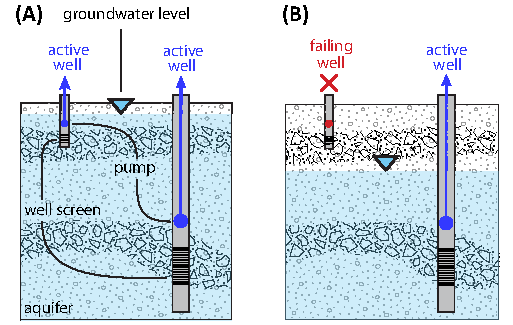
\includegraphics[width=\linewidth]{ch2_figs/fig_conceptual_mod.pdf}
	\caption{Conceptual model of well failure in an unconfined to semi-confined alluvial aquifer (details provided in SI Appendix, \ref{ap_a_formal_wf}). (A) Groundwater level is above all pump intakes, and all wells are active. (B) Groundwater level falls below the pump intake of the shallow well, causing it to fail. The deep well remains active. In our study site, shallow wells tend to be domestic, and deep wells tend to be agricultural and public supply wells.}
	\label{fig:conceptual_model_wf}
\end{figure}


%%%%%%%%%%%%%%%%%%% GW level interpolation
\subsection{Groundwater level interpolation}

Seasonal (spring and fall) groundwater level data for each year between 1998 and 2017 \citep{gwl} were used to determine groundwater level changes in the unconfined to semi-confined shallow aquifer, which domestic wells draw from. For each set of seasonal groundwater levels, we applied ordinary kriging to the log-transformed groundwater levels to normalize the data distribution, suppress outliers, and improve data stationarity \citep{DeutschC.V.andJournel1992, Varouchakis2012}. Because the expected value of back-transformed log-normal kriging estimates is biased (i.e. not equal to the sample mean), we applied the correction of Laurent \citep{Laurent1963, JournelA.G.Huijbregts1978} to recover unbiased groundwater level estimates (SI Appendix \ref{ap_a_gwl}). We further calculated the 5\% and 95\% confidence intervals of the kriging estimates to propagate kriging uncertainty through the model and into the well failure estimates.   


%%%%%%%%%%%%%%%%%%% Pump depth imputation
\subsection{Pump intake depth estimation}

Pump intake depth is not explicitly recorded on WCRs, thus for each well, it was estimated as the mean of the static water level at the time of well completion, and the top of the screened interval (SI Appendix \ref{ap_a_pump_depth}). When pump depth could not be directly calculated (i.e. - a WCRs is missing static water level or the top of the screened interval information), we imputed pump depths with simple linear models to regress known pump depths onto the bottom of the screened interval, which is known for nearly all wells (SI Appendix Figure \ref{fig:pump_loc_bottom}). Pump depth exhibits spatial variance due to geologic heterogeneity and historical groundwater level, hence imputation was conducted at the Bulletin 118 subbasin level (SI Appendix Figure \ref{fig:pump_loc_density}) to ensure hydrogeologic similarity. As with the kriging estimates, we calculated the 5 and 95\% confidence intervals of the estimated pump locations to propagate this uncertainty into the well failure estimates.    

%%%%%%%%%%%%%%%%%%% Calibration
\subsection{Model calibration based on 2012-2016 drought data}

The well failure model was calibrated with observed 2012-2016 well failures by relating groundwater level changes to estimated pump intake locations of wells in OSWCR, and minimizing error between the observed and predicted well failures during the 2012-2016 drought (SI Appendix \ref{ap_a_calib}). Well failures tend to form clusters, thus we calculated Gaussian kernel density estimates for the observed and predicted point patterns and calculated residual error as their difference. We use a kernel bandwidth of 433 $m$, calculated as $0.15 / \sqrt{5 \cdot \lambda}$ where $\lambda$ is the point intensity--the number of observations divided by the study site area \citep{stoyan1994fractals}. Calibration results are depicted at the Public Land Survey System \citep{us2009manual} township resolution (roughly 10 $km$) to improve mapping.




%%%%%%%%%%%%%%%%%%% drought duration scenarios
\subsection{Simulation of drought duration scenarios}

Climate change may cause severe and extended droughts exceeding 4 years in duration, yet the impact of such drought durations on domestic well failure remains unknown. Thus, we simulate drought durations of 5 to 8 years in length by extending the observed 2012-2016 drought with an additional 1 to 4 years using two scenarios:  

\begin{enumerate}
	\item \textit{Continuous drought}: 1 to 4 years of drought immediately following the 2012-2016 drought.
	\item \textit{Intervening wet winter}: identical to the continuous drought scenario, but groundwater levels are allowed to recover after 4 years, due to one intervening wet winter. 
\end{enumerate}

Groundwater level change in each drought duration scenario was determined by assuming that the impact of future droughts is proportional to the historical 2012-2016 drought. In other words, the groundwater level change associated with 1 to 4 additional years of drought is computed by scaling the change in the groundwater level field observed during the 2012-2016 drought by 0.25, 0.50, 0.75, and 1 respectively. 

In the ``continuous drought'' scenario, groundwater levels are already low from the 2012-2016 drought, and increased well failure is expected. Hence, the ``intervening wet winter'' scenario examines how much a wet winter event, such as the one observed in 2017, may buffer against well failure over a longer drought duration.  



%%%%%%%%%%%%%%%%%%% GW management regimes
\subsection{Projected groundwater management regimes}

In California, the Sustainable Groundwater Management Act (SGMA) enacted in 2014, requires the development and implementation of local groundwater management plans by 2020. These plans aim to prevent undesirable results, including the chronic lowering of groundwater levels, to achieve groundwater sustainability by 2040 for critically overdrafted basins.
%, and by 2042 for the remaining high and medium priority basins. 
Overlying landowners of overdrafted basins may deploy different groundwater management regimes, which will impact groundwater level change in the coming decades to various degrees.  

To analyze how different groundwater management regimes might impact groundwater level change and hence domestic well failure, we simulate three simplified regimes for the period 2017 -- 2040 (Figure \ref{fig:SGMAscenarios}): 

\begin{enumerate}
	\item \textit{Strict sustainability}: water levels do not decline after 2020. This represents a theoretical (and idealized) best case management regime for domestic wells.  
	\item \textit{Glide path}: groundwater level decline is gradually reduced over the implementation period until 2040.  
	\item \textit{Business as usual}: groundwater level decline continues at the historic rate. This regime is used for comparison.  
\end{enumerate}


% code/00_figures/alvar_scens
% .R and .ai files: pnas_sgma.ai
\begin{figure}%[tbhp]
	\centering
	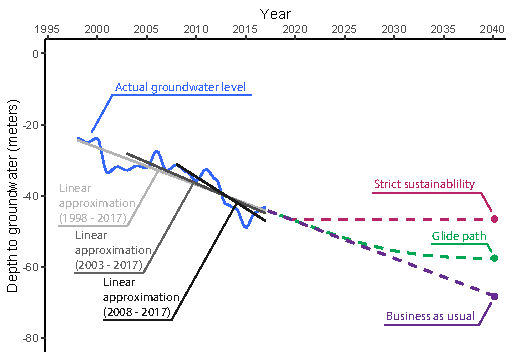
\includegraphics[width=\linewidth]{ch2_figs/fig_sgma.pdf}
	\caption{Projected groundwater management regimes using actual groundwater elevation change for a point in Tulare County as an example. Groundwater level change is approximated by three linear trends, based on different time periods. In this figure, we show the different projected groundwater management regimes using the linear approximation based on the 1998-2017 period. In the analysis, we calculate groundwater levels across the entire CV, using all three trends, and all three regimes.}
	\label{fig:SGMAscenarios}
\end{figure}

To project the number of failing wells for each groundwater management regime, we extend past groundwater level trends through 2040. For this, we first determined past groundwater level trends using data for the period from 1998-2017 and estimated annual groundwater levels at each point of the CV via ordinary kriging as discussed above and in SI Appendix section \ref{ap_a_gwl}. To estimate declining groundwater level trends consistently over time, we only use fall measurements following the growing season. We then obtain linear approximations of groundwater level for each cell using a 5x5 $km^2$ raster. We use three different approximations of groundwater level based on changes observed from 1998-2017, 2003-2017, and 2008-2017 to account for differences in initial groundwater level and thus, uncertainty introduced by the period over which the linear models are built. Finally, to project the ``Strict sustainability'' regime we extend these three approximations into 2020, then eliminate further overdraft. In contrast, the ``Business as usual'' regime projects the linear trends into 2040 before ending overdraft, and the ``Glide path'' regime gradually reduces the slope of the linear trend between 2020 to 2040, representing a middle path between the ``Strict sustainability'' and the ``Business as usual'' regimes. 




%--------------------------------------------------------%
% Results
%--------------------------------------------------------%
\section{Results}

\subsection{Well failure prediction during the 2012-2016 drought}

The calibrated model reproduced both the magnitude and spatial distribution of the 2,027 well failures observed in the study area during the 2012-2016 drought (Figure \ref{fig:pred_obs}A). The model predicts a slightly higher mean number of well failures (n = 2,513) (Figure \ref{fig:pred_obs}B), which is expected, as observed well failures are most probably under-reported due to the voluntary nature of data collection, and a well-owner's perceived consequence of reporting a failed well to their county or state. 

The normally distributed residual error (Figure \ref{fig:pred_obs}C) indicates the unbiasedness and strength of the model: well failure predictions for the observed 2012-2016 drought were within 20\% of the actual value for around 68.2\% of the study area, between 20\% and 55\% of the actual value for around 27.2\% of the study area, and greater than 55\% of the actual value for less than 5\% of the study area. 

Unsurprisingly, both observed and predicted failures tend to cluster in the southeastern CV, where agricultural groundwater use is comparatively higher than elsewhere in the state \citep{Brush2013, Faunted.2009}; households reliant on domestic wells in this region are particularly susceptible to failure. 


% 07_spatial_density_obs_and_pred.Rmd
% code/00_figures/pred_obs/pnas_pred_obs_accuracy.ai
\begin{figure}%[tbhp]
	\centering
	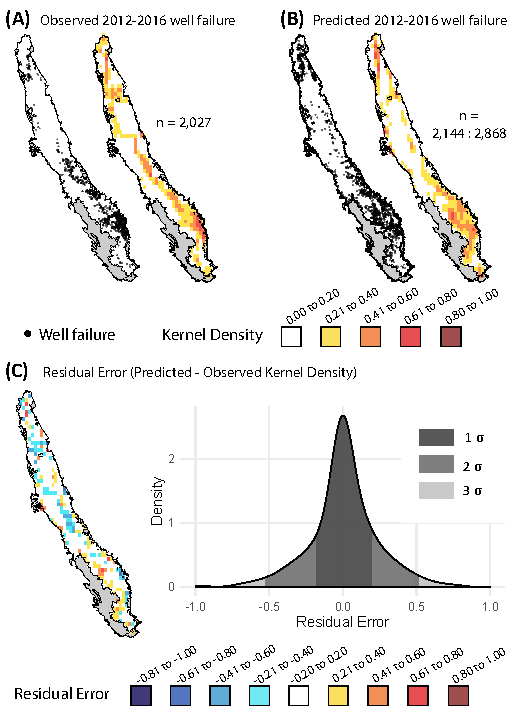
\includegraphics[width=14cm,keepaspectratio]{ch2_figs/fig_pred_obs_accuracy.pdf}
	\caption{Model performance in predicting the spatial intensity of observed domestic well failures during the 2012-2016 drought. (A) Observed well failure point pattern and kernel density estimate. (B) Predicted well failure mean estimate (n = 2,513) and kernel density of the mean prediction. The 5 and 95\% confidence intervals of predicted well failures span the interval from 2,144 - 2,868. (C) Residual (predicted minus observed) error, with red areas indicating areas of over-prediction, and blue areas indicating under-prediction.}
	\label{fig:pred_obs}
\end{figure}



%%%%%%%%%%%%%%%%%%% Drought duration scenarios
\subsection{Failing and vulnerable wells in drought duration scenarios}

Longer drought duration results in widespread well failure episodes concentrated primarily in the southeastern CV (Figure \ref{fig:p_1_2_3_4}). Consistent with domestic well failure patterns observed during the 2012-2016 drought, well failure density is highest in Madera, Kings, Kaweah, Tule, Tulare Lake, and Kern subbasins.  

% pred_1_2_3_4 in `09_plot_pred_future_failures.Rmd`
% density_pred_1_2_3_4 in `09_plot_pred_future_failures.Rmd`
% code/00_figures\pred_1_2_3_4/pnas_pred_1234_small_2.ai
\begin{figure}%[tbhp]
	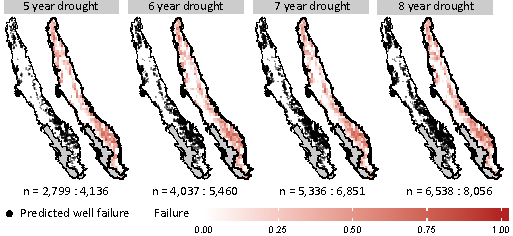
\includegraphics[width=\linewidth]{ch2_figs/fig_pred_1234_small_2.pdf}
	\caption{Simulated domestic well failure point patterns and associated kernel density estimates for 5 to 8 year drought duration scenarios beginning in Fall 2016 (maps show mean prediction). $n$ is the 5 and 95\% confidence interval of cumulative well failure count in each scenario, including the 2,027 failing wells in the 2012-2016 drought.}
	\label{fig:p_1_2_3_4}
\end{figure}

In the ``continuous drought'' simulation, two- and four-year long droughts immediately following the 2012-2016 drought (6 and 8 years total without an intervening wet winter) result in 4,037 to 5,460 and 6,538 to 8,056 cumulative well failures, respectively. Thus, a two-year drought duration following the 2012-2016 drought results in more well failures than the 2012-2016 drought alone, and a combined 8 year drought duration results in nearly twice the failures observed from 2012-2016 (Figure \ref{fig:cum_sum_failure}). Intensified well failure during extended drought reinforces the interdependence of well failure on groundwater level: when groundwater levels cannot recover to pre-drought levels and pump depths are fixed, wells are more vulnerable to failure.  

% `cum_sum_failures.pdf` in figures/code
% `p` in `13_trendline_d-2012_2016_and_future_d.Rmd`
% code/00_figures/cum_sum_fail/pnas_cum_sum_fail.ai
\begin{figure}%[tbhp]
	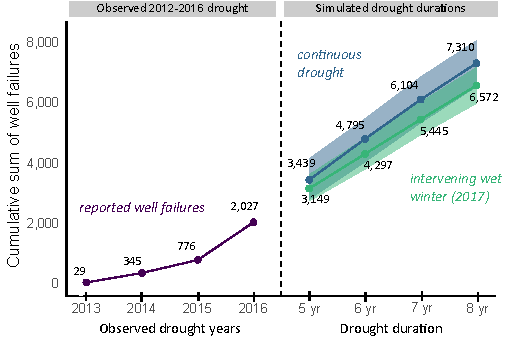
\includegraphics[width=\linewidth]{ch2_figs/fig_cum_sum_fail.pdf}
	\caption{Left: Cumulative domestic well failures from 2012-2016. Right: Cumulative domestic well failures resulting from simulated drought durations 5 to 8 years in length. The continuous drought duration scenario (blue) leads to more well failure compared to the intervening wet winter scenario (green). Points represent the mean well failure estimate, and shaded regions represent the 5 and 95\% confidence intervals. %Observed well failures from 2012-2016 reflect when the failure was reported, not necessarily when the well actually failed. Data collection by the state did not begin in a systematic way until late 2014, and many of the reports received in 2016 may be motivated by the fact that the state made financial assistance available to households on private wells in this year.
	}
	\label{fig:cum_sum_failure}
\end{figure}


In the ``intervening wet winter'' scenario, groundwater levels are allowed to recover during 2017, and well failure slightly abates: 498 and 738 fewer wells fail in the 6 and 8 year drought scenarios, indicating that an increase in median groundwater level of only a few meters across the Central Valley can prevent hundreds of domestic well failures during extended drought.  

%The cumulative sum of annual well failures observed during the 2012-2016 drought follows an exponential trend; in simulated extended drought scenarios, it follows a linear trend (Figure \ref{fig:cum_sum_failure}). If the drought were to continue past the simulated 8 years scenario, well failures would follow a sigmoidal trend: inflecting then leveling off, as failure progresses to increasingly infrequent and deeper wells until none are left.  

The cumulative sum of annual well failures observed in the evaluated drought duration scenarios follows a linear trend (Figure \ref{fig:cum_sum_failure}). If the drought were to continue past the simulated 8 years scenario, well failures likely would follow a sigmoidal trend: inflecting then leveling off, as failure progresses to increasingly infrequent and deeper wells until none are left.  

Vulnerable wells (Figure \ref{fig:vi}) are those with estimated pump intakes within 3 $m$ of the groundwater level, and are at heightened risk of experiencing a reduction in pump efficiency, or a failure episode. Since this 3 $m$ window is fixed in our analysis, the spatial distribution and count of vulnerable wells is relatively constant across the drought duration scenarios (2,274 to 2,453 wells), and the present day scenario of Fall 2018 (mean estimate = 2,568). Moreover, the spatial distribution of vulnerable wells mirrors those of well failures.

% figure starts in code/15_vulnerability_index.R
% 00_figures/vi/pnas_vi.ai 
\begin{figure}
	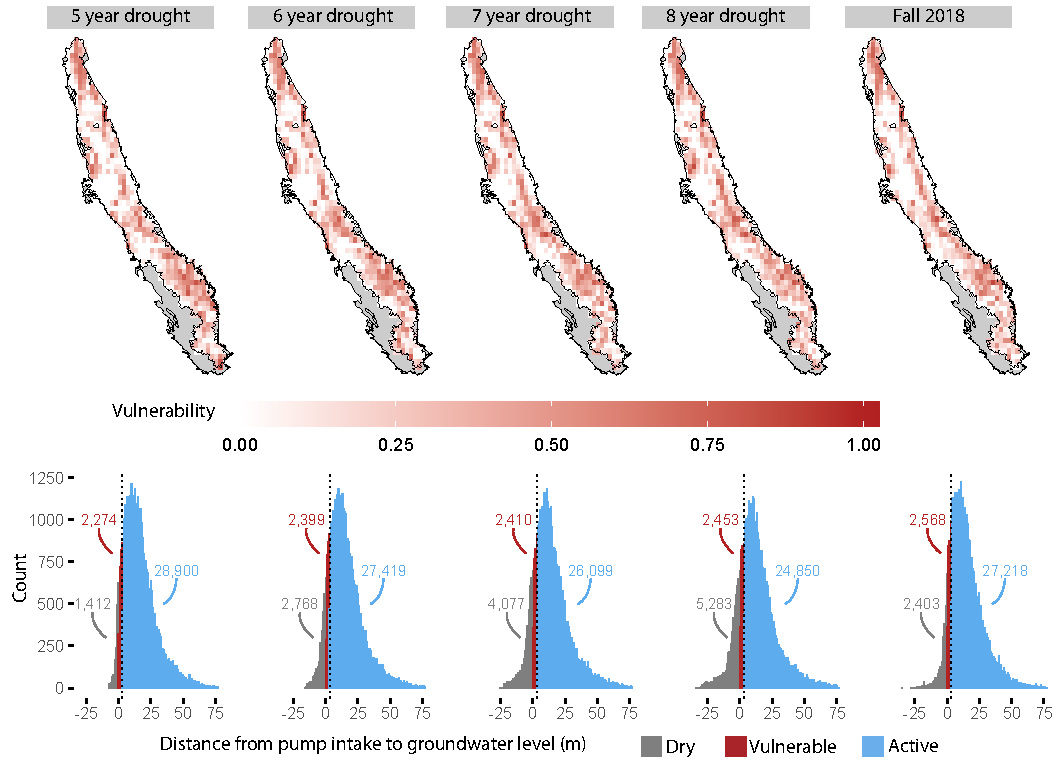
\includegraphics[width=17.8 cm]{ch2_figs/fig_vi.pdf}
	\caption{Top row: kernel density estimates of low vulnerability (white) and high vulnerability (red) regions in extended drought duration scenarios and in Fall 2018. Bottom row: histograms of failing wells (grey), vulnerable wells (red), and active wells (blue) for the extended drought scenarios and Fall 2018 scenario. The black dotted line at 3 meters is the threshold at which wells are at risk of decreased efficiency. All numbers reported are the mean estimate of dry, vulnerable, and failing wells.}
	\label{fig:vi}
\end{figure}



%%%%%%%%%%%%%%%%%%% sustainable management regimes
\subsection{Failing wells in projected groundwater management regimes}

Projecting groundwater depths into 2040 under three different management regimes results in significant differences in domestic well failures (Figure \ref{fig:sgma_grid}). The ``Business as usual'' regime, with no change in the historical trend of groundwater level decline, would lower the groundwater level by up to 100 $m$ in parts of the southern CV, but significant groundwater level declines are widespread. Scenarios aimed at achieving sustainability would reduce these declines, hence the differences between the ambitious ``Strict sustainability'', ``Glide path'' and ``Business as usual'' pathways might be quite important for water resources managers and policy makers.

The groundwater depth changes and associated well failures are sensitive to the period used for the linear approximation of groundwater level declines. The period from 2008-2017 leads to significantly worse groundwater depletion than both periods 2003-2017 and 1998-2017, particularly because of the effects of the 2012-2016 drought. Average well failures for the ``Business as usual'' regime range from 5,966 to 10,466 (depending on the period used for the linear interpolation), while under the ``Glide Path'' regime they range from 3,677 to 6,943, and from 1,516 to 2,513 under the ``Strict sustainability'' regime (confidence intervals are reported in SI Appendix Table \ref{tab:dom_failures}).  

% 18_run_model_2.R for simulation and plotting. paths below outdated.
% 00_figures/alvar_scens/pnas_sgma_grid_trim.ai
% 12_sustainable_gw_mgnt_scenarios.Rmd for:
% pnas_sgma_gwl_change.pdf | pnas_sgma_gwl_change_grid.pdf
% pnas_sgma_dry_wells.pdf | pnas_dry_well_grid.pdf
% 00_figures/alvar_sgma/sgma_scens.R for pnas_sgma_trends.pdf
\begin{figure}
	\includegraphics[width=17.8 cm]{ch2_figs/fig_sgma_grid_trim.pdf}
	\caption{Domestic well failures projected for three groundwater management regimes (columns) based on three different time periods of linear groundwater level change (rows). The left plot of each pair is the mean projected groundwater level change from 2017-2040. Groundwater level decline (red) is more common than groundwater level increase (blue). The right plot of each pair shows the mean predicted well failure point pattern for that combination of groundwater management regime and groundwater level change approximation. See SI Appendix Table \ref{tab:dom_failures} for confidence intervals.}
	\label{fig:sgma_grid}
\end{figure}
%TC:endignore
\clearpage

Most of the estimated domestic well failures are still concentrated in the southeastern CV, but the central and northern CV are also affected, presumably due to the ubiquity of relatively shallow wells in these regions. The ``Business as usual'' regime leads to especially severe well failure in all three projected groundwater level trends.



%--------------------------------------------------------%
% Discussion
%--------------------------------------------------------%
\section{Discussion}


%%%%%%%%%%%%%%%%%%% 
\subsection{Impact of drought duration on well failure and vulnerability}

It is well understood that drought duration leads to increased groundwater extraction \citep{Hanak2011, Medellin-azuara2016}, and hence domestic well failure \citep{Perrone2017, Feinstein2017}. Thus, we tested the impact of previously unseen drought durations ranging 5 to 8 years in length, by simulating an additional 2 to 4 years of severe drought immediately following the 2012-2016 drought, calculating the change in groundwater level, and determining failing and vulnerable wells. 

%Unlike existing regional-scale analyses \citep{Perrone2017}, the domestic well failure model developed in this study improves upon existing well failure models in terms of spatial scale \citep{Gailey2019}, and allows for scenario testing. 
A previous study estimated that 4 years of drought in the Tulare County, California immediately following the 2017 wet winter would result in about 200 - 850 domestic well failures \citep{Gailey2019}. 
Our model's equivalent scenario (intervening wet winter with an 8 year drought duration) results in a similar range of 585 - 715 domestic well failures in Tulare County. Additional comparisons are not possible given the lack of research on this topic.  

At the level of California's CV, our results suggest that drought durations of 6 to 8 years result in 4,037 to 5,460 and 6,538 to 8,056 cumulative well failures, respectively. However, an intervening wet winter during the 6- and 8-year long drought duration simulations buffers against well failure: when groundwater is allowed to recover after 4 years of drought (as happened during the 2017 wet winter), an average of 498 and 738 less domestic wells fail. These findings support research indicating that limiting groundwater pumping during drought may reduce well failure \citep{Hanak2019, Gailey2019}, and a general understanding that groundwater pumping can lower proximal groundwater levels \citep{theis1935relation}.  

During the 2012-2016 drought, the median groundwater level in the CV fell to progressively new historic lows each fall after the summer growing season (SI Appendix \ref{ap_a_drought_impact}) \citep{dwrgwl2017}. Our results indicate that between fall of 2014 and 2015, the median groundwater level across the entire CV fell by nearly 5 $m$, and in some areas (i.e. - Tulare, Kings, and Kern counties), by tens of meters. In fall of 2016, the median groundwater level in the CV was 27.0 $m$ below land surface. Moreover, our results indicate that the interquartile range of domestic well pump locations in the CV is 24.5 to 52.3 $m$ below land surface. The proximity of pump intake depths to groundwater levels explains why domestic wells are sensitive to even slight declines in groundwater level: 5 to 10 $m$ of groundwater level decline may easily impact thousands of domestic well pump intakes and cause failure. 

In the four drought duration scenarios evaluated, an average of 2,274 to 2,453 domestic well pumps reside within 3 $m$ of the groundwater level. We classified these wells as vulnerable, because they are likely to fail first under persistent groundwater level decline. The spatial distribution of well vulnerability mirrors that of well failures. Mapping clusters of predicted failing and vulnerable wells is essential for sustainable water management and disaster response.


%%%%%%%%%%%%%%%%%%% 
\subsection{Implications for groundwater management and policy}

The strong dependence of domestic well failure on groundwater pumping to support irrigated agriculture raises serious questions concerning the role of sustainable groundwater policy in mitigating well failure \citep{Hanak2019}. We evaluated three different projected groundwater management regimes to curb groundwater level declines in the coming years: a ``Strict sustainability'' theoretical best-case regime wherein declining trends in groundwater level stop in 2020, a ``Business as usual'' regime that continues groundwater decline until 2040, and a final ``Glide path'' moderate regime that slows the rate of groundwater level decline to the midway point between the former two regimes.  

Our results suggest that choices embedded within each of the groundwater management regimes vastly impact the amount of expected well failures. For instance, the ``Glide path'' regime predicts 3,677 to 6,943 domestic well failures by 2040, and the ``Business as usual'' regime predicts 5,966 to 10,466 domestic well failures by 2040. Both groundwater management regimes would result in twice to almost three times as many well failures than the ``Strict Sustainability'' regime (1,516 to 2,513 failures). All three scenarios are sensitive to the period of record used to approximate the linear groundwater level decline, however they underpin the vulnerability of domestic wells to historic rates of groundwater level decline, and demonstrate the impact of management on well failure.  

Refilling overdrafted aquifers via managed aquifer recharge might meet the dual objectives of increasing groundwater storage, and bolstering domestic well dependent households' drought resilience. In California, high-magnitude flood flows are likely the most accessible and largest sources of water to replenish groundwater aquifers through managed aquifer recharge \citep{Kocis2017}, which might considerably slow or reverse trends in groundwater depletion. The emerging research in the strategic siting of managed aquifer recharge considers impacts on crop health \citep{Dahlke2018}, human health \citep{ayuso2011quantifying}, the mobilization of contaminants into groundwater \citep{Xanke2017}, and hydrogeologic suitability (i.e. - highly conductive flowpaths and geologic formations capable of accommodating large volumes of water, such as incised valley fills) \citep{Maples2019}. In the San Joaquin Valley where domestic well failures peak, managed aquifer recharge alone may not be enough to offset groundwater overdraft, but coupled with a reduction in agricultural water use \citep{Hanak2019}, groundwater levels may stabilize enough to prevent widespread future failure events. 

This study assumes that no interim well construction takes place to prepare for falling groundwater levels, such as the practice of pump lowering or well deepening. Pump lowering typically takes place in 6 $m$ intervals (the length of standard discharge piping), and costs around \$2,000 USD per lowering event \citep{Gailey2019}. If we consider the cost of pump lowering in all failing wells in the 6- and 8-year drought duration scenarios (in reality some wells will not have room to be lowered) and assuming every failing well's pump is lowered once (some will require more than one lowering), at \$2,000 USD per 6 $m$ unit of discharge piping, 4,037 - 5,460 and 6,538- 8,056 failures correspond to \$8.7 - \$10.4 and \$13.8 - \$15.5 million USD. 

During the recent drought, it is likely that some households also deepened their wells. In California and nationwide, drilling deeper wells is a common practice to adapt to declining groundwater levels \citep{Perrone2019}, but is a costly and unsustainable solution that may furthermore result in cross-contamination due to interconnection of confined aquifers by well construction \citep{gailey2017inactive}. Moreover, the financial burden of pump lowering or well deepening might disproportionately impact disadvantaged populations \citep{Famiglietti2014} unable to afford chasing after declining groundwater levels. Since many of these disadvantaged groups may not own their land and thus wells, well construction decisions may be made by landowners rather than the affected groups.  

%%Underpinning the dilemma of domestic well failure is the urgent need for an adequate cost estimation to facilitate sensible short- and long-term policy solutions. 
Sustainable long-term solutions for drinking water access might include connecting vulnerable households to nearby centralized water provisions. Recent research indicates that many rural communities, assumed to be on domestic wells, are actually quite close (less than 2 $km$) to a potable water supply system \citep{London2018}. However, as annexation and consolidation is financially and physically impractical for all domestic-well dependent households, many will remain too remote and isolated to connect to a nearby water system.  

%We currently lack a thorough understanding of the economic burden of well failure and how it may affect demographic groups disproportionately. 
Short- and long-term solutions to domestic well failure remain largely unexplored. What role can managed aquifer recharge play in mitigating well failure? Given the strong dependence of groundwater level decline on extraction for irrigated agriculture, could agri-business proximal to centers of high well failure collectively fund safety nets that internalize the cost of well failure during periods of increased groundwater pumping? Should vulnerable domestic well reliant populations connect to nearby municipal water systems with more reliable water supply? What is the appropriate solution for those that are too remote or isolated to connect to a community system? 

%%%%%%%%%%%%%%%%%%% 
\subsection{Applicability to other areas}

The well failure model presented in this study is extensible to other areas outside of California where sufficient data or groundwater flow models are available. It relies on two inputs: (1) a time series of spatially-explicit groundwater level surfaces reflecting typical groundwater level changes (specifically, the maximum drawdown), and (2) well construction information (i.e. - geographic location and pump intake depth). 

Approaches for interpolating groundwater levels and estimating pump intake depths are demonstrated in this study, though others exist \citep{Gailey2019, Perrone2017, OSullivan2010, JournelA.G.Huijbregts1978}. Groundwater levels provided by a groundwater flow model such as MODFLOW \citep{Harbaugh2000} would easily couple to a well failure model, enabling the simulation of water management regimes and the impact of the resulting groundwater level on domestic well failure at arbitrary temporal scales. In California, existing regional-scale groundwater flow models such as C2VSim \citep{Brush2013} and CVHM \citep{Faunted.2009} can be used to plan for the impact of future failure episodes under different water management regimes involving changes in both pumping and recharge in space and time. 

This study aimed for regional prediction of failing, vulnerable, and active wells, but more nuanced impact analyses can be made. For instance, variable losses in well efficiency may be quantified as groundwater levels fall \citep{Medellin-azuara2016}. This in turn enables the cost estimation of repairing failing and vulnerable wells (e.g. - pump lowering, well deepening), compared to water management actions (e.g. - fallowing fields, reduced groundwater pumping).  

Where resources exist to survey households, detailed domestic well information such as geographic location, pump intake depth, and retirement age may be obtained, and would further constrain the uncertainty inherent in the estimation of these parameters. Additionally, well failure observations are essential for model calibration. Though this study benefited from failure data, efforts to anticipate domestic well failures as proactive hazard mitigation should not wait for the existence of observational data. It does, however, suggest the benefit of having such a system in place as part of local and state-level drought preparedness.  

%%%%%%%%%%%%%%%%%%% 
\subsection{Implications for adaptation to climate change}

Our results demonstrate that the mechanisms leading to domestic well failure are heavily dependent on groundwater level declines due to pumping for irrigated agriculture and increased pumping during drought. A historical lack of groundwater management in California \citep{Hanak2011} has led to widespread groundwater level decline. Climate change compounds the impact of water management decision-making. Warming will increase the frequency and duration of drought in California and other parts of the world \citep{Diffenbaugh2015, Cook2015, Swain2018, Rhoades2018, VanLoon2016}, and if left unchecked, groundwater withdrawal will likely intensify as surface water becomes more scarce, as it has in the past \citep{Hanak2011}. As we demonstrate in this study, groundwater replacement of lost surface water during extended drought intensifies well failure due to already low groundwater levels. Thus, managing for low to no domestic well failure requires a consideration of the complex interaction between land use change, water resources management, human decision-making, and climate change. Unless adaptation strategies become integral to sustainable groundwater management policy, the extended droughts anticipated under climate change and resulting changes in groundwater levels will put thousands of domestic wells in California's CV at risk of failure, and hence, thousands of Californians at risk of losing access to water.  


%%%%%%%%%%%%%%%%%%% 
\subsection{Additional perspective on the data and model}

%% This study is one example of how state-led initiatives towards open data, or the practice of releasing previously-private databases to the public, enables research towards previously inaccessible questions. This study benefited from open data tabulated in a machine-readable format, which simply would not have been possible otherwise. By comparison, while former studies have dedicated many hours to statistically sample and manually read nearly three quarters of a million WCRs \citep{Johnson2015}, we were able to automate the reading and QAQC process for nearly one million tabulated WCRs. This reinforces existing and nascent efforts to transition data-collection and storage to standardized, digital, and machine-readable formats that can be easily accessed and manipulated by scientific scripting languages.  

There is generally good agreement between the observed and predicted well failure at the 10 $km$ resolution of the residual error maps (Figure \ref{fig:pred_obs}A-B), and better agreement (Figure \ref{fig:pred_obs}C) is achieved at larger spatial scales (i.e. - Bulletin 118 groundwater subbasins, entire CV). Thus, the results presented in this study should not be taken as \textit{de facto} predictions of the exact locations of well failure, but rather, as \textit{regional-scale} well failure estimates. Local-scale errors introduced by uncertainty in well failure reporting, well completion reporting, groundwater level, and model formulation are overcome at regional scales. 

We acknowledge that spatial and temporal variability in monitoring well data introduces uncertainty in the interpolated groundwater level. Ambient monitoring wells measured each season (i.e. - spring and fall) are not the same across seasons, and each season's measurements are sampled over a roughly three month time frame (January-March in the spring, and October-December in the fall). However, because most of the groundwater level change observed in a year takes place as the result of the summer growing season, and the fall measurements take place after the summer, spring and fall measurements still reflect ambient conditions. Moreover, both scaling the 2012-2016 groundwater level change to create future drought scenarios, and calculating 2040 groundwater levels with linear trends are simple approaches to estimate future groundwater level decline, but the accuracy of any method to forecast unseen future events are also questionable. Additionally, we do not account for any emergency response measures in response to drought such as groundwater pumping curtailments. In California, some households were able to drill deeper wells, lower their pumps, or connect to a nearby surface water supply system during the drought. Because these corrective actions are cost-prohibitive and highly unlikely to be widespread, our modeling assumptions (no corrective action) and hence results, still agree with observed well failure rates from 2012-2016. 




%--------------------------------------------------------%
% Conclusion
%--------------------------------------------------------%
\section{Conclusions}

%% More than one million Californians rely on private domestic wells for drinking water, and nearly half a million of these people live in the CV. Owing to their relatively shallow depth, domestic wells often fail first when groundwater levels fall, as observed during the 2012-2016 drought. As water resource managers aim to stabilize groundwater level declines, climate warming threatens to increase drought frequency and duration in California. We currently lack drought preparedness tools for regional-scale estimation of domestic well failure, and the ability to rapidly assess future well failure under different groundwater level scenarios. 

In this study, we developed a data-driven well failure model and applied it to California's CV to make regional-scale estimates of domestic well failure, and assess future well failure under different groundwater level scenarios.  

Our model reproduces reported domestic well failures during the 2012-2016 drought in California's CV ($n$ = 2,027), and furthermore, simulates the impact of different drought duration scenarios up to 8 years in length. We show that small declines in groundwater level are sufficient to cause thousands of wells failures when groundwater levels are already low, and that wet winters, and hence groundwater recharge or reduced pumping, may buffer against well failure. A simulated drought duration of 6 years (2012-2018) results in 4,037 - 5,460 total well failures. Similarly, an 8-year long drought (2012-2020), corresponds to a median groundwater level change of less than 10 $m$ across the CV, but results in 6,538- 8,056 total well failures. The same 6 and 8 year long drought duration scenarios with an intervening wet winter in 2017 lead to an average of 498 and 738 fewer well failures. Lastly, wells that do not fail may still be vulnerable to failure. Our model estimates that in Fall 2018, an average of 2,568 well pump intakes were within 3 $m$ of the groundwater level, and 10,544 well pump intakes were within 10 $m$ of the groundwater level. 

Our model further shows that early adoption of sustainable groundwater management regimes aimed at halting declining trends in groundwater level will lessen the magnitude of domestic well failure. A ``Business as usual'' linear groundwater level decline would result in an average of 5,966 - 10,466 domestic well failures by 2040. In contrast, a more gradual ``Glide path'' decline would result in 3,677 - 6,943 domestic well failures by the same date. A ``Strict sustainability'' regime that allows groundwater levels to decline until 2020 before halting would result in 1,516 - 2,513 well failures.  

Together, these results demonstrate that access to domestic water supply for large rural populations may be imperiled by a relatively small number of agricultural users, posing challenges for equitable and sustainable groundwater management which may not adequately represent domestic well users. 

Models like the one developed in this study may be updated over time to accommodate additional wells, refine existing well construction information, and evaluate the impact of potential water management strategies on groundwater level changes, and hence well failure. This study's approach to well failure modeling may be applied in other arid regions worldwide to facilitate drought preparedness planning. We anticipate that the model developed herein may be used by local and state agencies developing groundwater management plans in accordance with California's Sustainable Groundwater Management Act.  

\clearpage
 %This looks for chapter2.tex
%%%%%%%%%%%%%%%%%%%%%%%%%%%%%%%%%%%%%%%%%%%%%%%%%%%%%%%%%%%%%%%%%%%%%%%%%%%%
\section{Supporting Information Appendix} \label{ap_a_dom_wells}

\subsection{Study Area}
\label{ap_a_study_area}

The study area was pared down from the Central Valley (CV) to only the area where more recently completed domestic wells (1976 and younger) were present. This cutoff was chosen because the model period in this study ends in 2016, thus wells completed on or after 1976 ($n = 67,011$) assumes a conservatively high well retirement age of 40 years. Circular, 5 $km$ buffers were drawn around each well, then joined to create a unified study area polygon. Some isolated circles that were not connected to any other buffers ($<$ 1\% of the buffered area) were removed in order to constrain the study site to one contiguous spatial extent in the CV corresponding to the areas of greatest domestic well density. The small removed areas principally occur in the western San Joaquin Valley. Low rates of domestic well completion in the west side of the San Joaquin Valley compared to the CV as a whole are explained by a relatively deep water table, poor shallow groundwater quality, and perhaps missing well completion records in places where there are actually households on unregistered or non-permitted domestic wells. 


%%%%%%%%%%%%%%%%%%%%%%%%%%%%%%%%
\subsection{Data}
\label{ap_a_data}

The California DWR keeps paper records of wells drilled in California that contain well construction information, such as the depth of the well, perforated interval dimensions, location, and well type (e.g. - irrigation, domestic, monitoring, etc.) among other data. These records are submitted by the well-drilling company to the state in the form of a Well Completion Report (WCR). Nearly all WCRs in the state have been digitally scanned, and key fields in the reports have been digitized. Until recently, WCR information was confidential under state law, and they were unavailable to the general public, limiting researchers' abilities to answer questions like those set forth in this study.

The State’s Household Water Supply Shortage Reporting System (HWSSRS) was established in late 2014 as a tool to capture information on water supplies running dry due to worsening drought conditions across California. The data gathered by the system was used for coordinating the State’s drought emergency response efforts.  The system was set up as a voluntary, self-reporting system and, as such, only represents some fraction of the actual water supply shortages occurring. Most of the reported shortages were dry wells, but some were streams. Most of the reports were actually received by county health officials who entered the data into the system. Some counties were very active in reporting, while some were not. A download of the reported HWSSRS data has been made available to researchers with redaction of some data fields and a reduction in the accuracy of geospatial data to protect personal identification. The precision of the geospatial data is 36 arc seconds, corresponding to approximately 1 $km$ in the study area. The coordinate reference system used in this study is EPSG 4326.  

The great majority of well locations in OSCWR ($>$ 95\%) are rounded to the nearest centroid of the Public Land Survey System (PLSS) section. The PLSS is composed of a nested series of cadastral surveyed lands (e.g. townships, range and sections). Townships measure 6x6 square miles (93.24 $km^2$ each) in size and are made up of thirty-six one-square mile sections (2.56 $km^2$). As the distance between the cell centroid and a corner of each section is the half-diagonal $0.5\cdot\sqrt{2}\cdot1.6 = 1.14$ $km$, the reported location \textit{(x, y)} of each well is always 0 $\leq$ \textit{(x, y)}  $\leq 1.14$ $km$ from the true location. Determining the exact location of a well from the scanned well completion reports is intractable as well coordinates are rarely provided on the scanned forms, and the listed street address typically corresponds to the well owner's residence, not necessarily where the well is located, thus hampering efforts at geocoding. Due to these limitations, the reported PLSS section centroid was taken as the approximate well location, with a maximum error of 1.14 $km$.

%%%%%%%%%%%%%%%%%%%%%%%%%%%%%%%%
\subsection{Formal evaluation of well failure}
\label{ap_a_formal_wf}

Classification into active wells and failing wells proceeds through several steps (Figure \ref{fig:tree}). Consider a well $i$. It has a set of spatial coordinates and an associated estimated pump depth $(x_i,y_i,z_i)$, where $x_i$ and $y_i$ are the Cartesian coordinates, and $z_i$ is the estimated depth of the pump within the well casing that draws water from the surrounding aquifer. The groundwater level $g$ is a scalar field which varies by location; the groundwater level at a well is thus a scalar defined by its coordinates: $g_i = f(x_i,y_i)$. We determine the groundwater level for some initial time $g({t_0})$ and final time $g({t_f})$ at each location in the study area by ordinary kriging.  

% tree diagram of well failure
\begin{figure}[ht]%[tbhp]
	\includegraphics[width=\textwidth]{ch2_appendix_figs/tree.png}
	\caption{Decision tree representing the steps taken to evaluate active and retired wells, initially active and well failures, and finally, active wells and well failures given the following boundary conditions: retirement age, initial groundwater level, and final groundwater level.}
	\label{fig:tree}
\end{figure}

Classification into active and failing wells proceeds as follows. Let the set of all domestic WCRs be called $W$. First, wells with age $a$ greater than or equal to the calibrated retirement age $t_r$ (Section \ref{ap_a_calib})
 are removed from the simulation. 
%(see section \ref{ss_2_6} for a discussion of how this parameter is determined). 
This yields two sets: the initial wells to consider ($W_i$), and the retired wells ($W_r$).  

$$W_i \subseteq W : a_i \leq t_r$$  

$$W_r \subseteq W : a_i > t_r$$  

The remaining active wells at this point are the initial wells to consider, $W_i$. However a well may not be active at $t_0$ frame if its pump is above the groundwater level at $t_0$. Next, wells with pumps above the groundwater level at the start of the simulation were removed, yielding another two sets: the active wells at time zero $W_a(t_0)$, and the failing wells at time zero $W_d(t_0)$. 

The active wells at time zero are the subset of initial wells to consider where the groundwater level at time zero $g({t_0})$ at the location of the well exceeds the pump depth $z$, and the failing wells at time zero are the wells where the groundwater level at time zero at the location of the well falls at or below the pump depth.  

$$W_a(t_0) \subseteq W_i : g({t_0}) > z$$  

$$W_d(t_0) \subseteq W_i : g({t_0}) \leq z$$

Lastly, the groundwater level field at the final time $g({t_f})$ is applied, yielding the final two sets of wells: well failures $W_d(t_f)$ and active wells $W_a(t_f)$. Well failures are the subset of wells where the final groundwater level at the location of the well falls at or below the level of the pump, and active wells are the subset of wells where the final groundwater level at the location of the well does not fall below the level of the pump.  

$$W_a(t_f) \subseteq W_0 : g({t_f}) > z$$  

$$W_d(t_f) \subseteq W_0 : g({t_f}) \leq z$$  

$W_d(t_f)$ and $W_a(t_f)$ combined form the set of all active wells at time zero $W_a(t_0)$. 

Taken together, the three steps taken to classify wells into active and failing wells are visualized as a decision tree in Figure \ref{fig:tree}.  


%%%%%%%%%%%%%%%%%%%%%%%%%%%%%%%%
\subsection{Vulnerable wells}
\label{ap_a_vi}

Vulnerable wells are defined as wells that may experience a loss in function due to sufficiently low water levels above the estimated pump intake depth. We estimate that 3 $m$ is the threshold at which a well may experience losses in function, based on a pumping rate of 1 $m^3 / hr$, a required net positive suction head of 5 $m$, a barometric pressure head of 10 $m$ (at 25 degrees C and 0 $m$ above mean sea level), a vapor pressure (at 25 degrees C) of 0.3 $m$, and friction head losses of 1 $m$ \cite{Tullis1989}. 


%%%%%%%%%%%%%%%%%%%%%%%%%%%%%%%%
\subsection{Groundwater level interpolation}
\label{ap_a_gwl}

The groundwater level interpolation consists of five steps: (i) data collection; (ii) log transformation; (iii) ordinary kriging; and (iv) back-transformation and correction of the interpolated groundwater levels.  
Groundwater level data covering fall and spring measurements between 1998 and 2017 were obtained from DWR \cite{gwl}. Seasons are defined as either spring (January - March) or fall (August - October). Groundwater levels in a season reflect the ambient signal of the unconfined to semi-confined aquifer. Groundwater levels are measured in reference to the land surface at the measurement locations.

Many environmental data follow a log-normal distribution \cite{Stedinger1980}, including the ambient groundwater levels used in this study. Depths to groundwater at each monitoring well were log transformed ($ln(x)$) prior to interpolation to normalize the data distribution, suppress outliers, and improve data stationarity \cite{DeutschC.V.andJournel1992, Varouchakis2012}. 

Ordinary kriging was then used to interpolate groundwater levels for each season. Inverse distance weighting and thin plate splines were also considered, but discarded because they produced unrealistic groundwater levels near the study area's boundaries, where conditioning data was sparse, and unlike kriging, are susceptible to bulls-eye patterns (concentric areas of equal value around known data points).  
%The interpolation techniques used in this study are well documented (e.g. \cite{JournelA.G.Huijbregts1978}) and beyond the scope of this paper. 
Ordinary kriging parameters were determined by fitting an exponential semi-variogram model. 

Since the expected value of back-transformed log-normal kriging estimates is biased (i.e. - not equal to the sample mean), we apply a correction \cite{Laurent1963, JournelA.G.Huijbregts1978}:  

\begin{equation}
    g = k_0 \cdot exp \Big[ ln(\hat{g}_{OK}) + \frac{\sigma^2_{OK}}{2} \Big]
\end{equation}

Where $g$ is the corrected and back-transformed groundwater level, $\hat{g}_{OK}$ is the ordinary kriging estimate, $\sigma^2_{OK}$ is the kriging variance, and $k_0$ is the correction factor, proportional to the ratio of the mean of the sample values to the mean of the back-transformed kriging estimates.  

Lastly, the the 5 and 95\% confidence intervals of the kriging estimate was determined via: $\hat{g}_{OK} \pm (1.96 \cdot \sqrt{(\sigma^2_{OK})})$. These confidence intervals are propagated through the model to account for uncertainty in the estimated groundwater level.   


%%%%%%%%%%%%%%%%%%% GW levels
\subsection{Impact of drought on seasonal groundwater levels}
\label{ap_a_drought_impact}

Interpolated seasonal groundwater levels in the study area during the 2012-2016 drought exhibit oscillating seasonal variation between spring and fall, a downward trend as the drought progresses from spring 2012 to fall 2015, and an upward trend beginning in spring 2016 and continuing into 2017. Seasonal groundwater level oscillation is a byproduct of agricultural groundwater demand, which peaks during summer and fall months. 

% gw_boxplot_sp_fall in `02_interpolate_all_seasons_GF.Rmd`
% sp_fa_gwl in `06_calibartion_herve_alvar_graham.Rmd`
% sp_fa_gwl.ai in code/00_figures/sp_fa_gwl/pnas_sp_fall_gwl.ai
\begin{figure}[ht]%[tbhp]
	\includegraphics[width=\textwidth]{ch2_appendix_figs/erl_sp_fa_gwl.pdf}
	\caption{Groundwater levels during the most intense 4-year period of the 2012-2016 drought in (A) spring 2011, and (B) fall 2015. (C) Box plots showing the median and 25\% and 75\% percentiles of depth to groundwater. Compared to spring groundwater levels, fall levels tend to be deeper. The schematic assumes that groundwater levels do not decrease with depth, which is not a concern for most of the domestic wells because they tend not to be very deep.}
	\label{fig:sp_fall_gwl_2}
\end{figure}

The median groundwater level oscillates with the growing season (Figure \ref{fig:sp_fall_gwl_2}C) and is generally higher in spring than in fall of the same year. Between spring and fall of 2015 alone, the median groundwater level across the CV fell by nearly 5 $m$. In that same water year, Sierra snowpack measured at an all time low of 5\% of the average snowpack \cite{cadwr2017}, implying that low snowpack leads to more groundwater pumping and hence a seasonal lowering of groundwater levels. 

Median groundwater levels decline between spring 2012 and fall 2015, the four driest consecutive years on California's record (Figure \ref{fig:sp_fall_gwl_2}C). These groundwater level declines coincide with more pumping, which is due to less surface water delivered, which is due to less snowpack. In 2015, California set state records for high temperature, low precipitation, and low snowpack \cite{cadwr2017}. Median groundwater levels start trending upwards in spring 2016 and into 2017, indicating the easing of groundwater pumping. This inflection coincides with the relative return of the Sierra snowpack: in the 2016 and 2017 water years, Sierra snowpack was 85\% and 159\% of normal \cite{cadwr2016, cadwr2017}.  

Over the course of the drought, groundwater levels decline most evidently in the southern CV (i.e. - Madera, Kings, Kaweah, Tule, Tulare Lake, and Kern Bulletin 118 subbasins). These findings are consistent with former research indicating that the central and southern CV experienced the largest surface water loss and groundwater replacement in 2016 \cite{Medellin-azuara2016}, and estimates that California replaced more than 70\% of lost surface water supply with groundwater during the 2012-2016 drought \cite{Lund2018}. 


%%%%%%%%%%%%%%%%%%%%%%%%%%%%%%%%
\subsection{Pump intake depth estimation}
\label{ap_a_pump_depth}


The depth of the pump intake in each domestic well, henceforth called the pump depth ($z$), was estimated for all wells ($W$) as the mean of the static water level at the time of well completion, and the top of the screened interval. This assumption is based on the fact that well pumps are submerged upon installation, and the mean of the static water level at the time of well completion and top of the screened interval represents an unbiased best estimate of where the pump was likely to be placed. Pump depth could not be directly calculated for wells missing either the static water level or the top of the screened interval. Moreover, pump depth exhibits spatial variance due to geologic heterogeneity and historical groundwater use (Figure \ref{fig:pump_loc_density}), which suggests the need for imputation as a function of spatial location. Thus, simple linear models were developed for all wells located within a Bulletin 118 subbasin relating the logarithm of pump depth $z$ to the logarithm of screen bottom, $z_{b}$ (Figures \ref{fig:pump_loc_bottom}-\ref{fig:north_south_impute}). 

\begin{equation}
  log(z) = \beta_{0} + \beta_{1}log(z_{b}) + \epsilon
\end{equation}

Conveniently, $z_{b}$ is known for nearly all wells in the study area. Where it was unknown, it was taken as the total completed depth. Linear models for each subbasin were used to impute the pump depth for wells missing either static water level, top of screened interval, or both.  

%% Distribution of pump depth in B118 SB for data-dense basins (n > 75)
%% pump_loc_density.pdf in `08_pump_loc_spatially_varying.Rmd`
\begin{figure}
	\includegraphics[width=\textwidth]{ch2_appendix_figs/erl_pump_loc_density.pdf}
	\caption{Density distributions of estimated pump intake depth for a subset of 16 Bulletin 118 subbasins. The red vertical line indicates the mean pump depth.}
	\label{fig:pump_loc_density}
\end{figure}

% linear model data clouds and line of best fit
%% p_pump_loc_bot.pdf in `08_pump_loc_spatially_varying.Rmd`
% touched up in code/00_figures/pump_loc_bot/ ... ai
\begin{figure}[ht]
	\includegraphics[width=\textwidth]{ch2_appendix_figs/erl_pump_loc_bot_eq.pdf}
	\caption{Relationship between the logarithm of pump depth ($z$), and logarithm of the bottom of the screened interval ($z_{b}$) for a subset of 16 Bulletin 118 subbasins.}
	\label{fig:pump_loc_bottom}
\end{figure}

% map of data dense basins, data poor basins, SBs used to construct linear models, and lines of best fit
%% north_south_impute.png in `08_pump_loc_spatailly_varying.Rmd`
\begin{figure}[ht]
	\includegraphics[width=\textwidth]{ch2_appendix_figs/erl_north_south_impute_eq.pdf}
	\caption{(A) Count of wells per Bulletin 118 subbasin with recorded screen bottom and directly estimable pump depth, further classified into northern and southern subbasins. (B) \& (C) Northern and Southern subbasins used to construct the linear relationships between pump depth and screened interval bottom; the wells within are shown as black points. (D) \& (E) Northern and Southern linear models used to impute pump depth for northern and southern basins with fewer than 75 samples.}
	\label{fig:north_south_impute}
\end{figure}

Pump depth estimates were generally poor in Bulletin 118 subbasins with fewer than 75 wells, such as in the western San Joaquin Valley, and in various subbasins from the Sacramento Valley to the northernmost CV (Figure \ref{fig:north_south_impute}A). To improve pump depth estimates in these regions, we used observations from adjacent subbasins (Figures \ref{fig:north_south_impute}B \&  \ref{fig:north_south_impute}C) to construct linear models relating pump depth and screen depth as described above (Figures \ref{fig:north_south_impute}D \&  \ref{fig:north_south_impute}E).  

The 5 and 95\% confidence intervals for each linear model were calculated via the standard approach \cite{james2013introduction}, and propagated through the model to account for uncertainty in the estimated pump location.   


Distributions of estimated pump intake depth at the DWR Bulletin 118 subbasin level tend to be either normal or left-skewed (Figure \ref{fig:pump_loc_density}), indicating that most pumps are shallow and close to the land surface. The mean estimated pump depth across subbasins ranges from 25.44 $m$ in the North American subbasin to 68.84 $m$ in the Madera subbasin, suggesting that many pumps are, within tens of meters of the land surface. Considering that most groundwater levels are also tens of meters below land surface %(Figure \ref{fig:sp_fall_gwl_2})
, the distance between a particular well's pump and the upper groundwater level may be only a few meters. Consequently, small groundwater level declines of only a few meters during a drought can lead to considerable domestic well failures.  

The strong relationship between the bottom of the screened interval and the estimated pump depth (Figure \ref{fig:pump_loc_bottom}) was a useful approach for imputing missing pump depths. Goodness of fit ($r^2$) for subbasins have a median of 0.84, and range from 0.93 to 0.41. Residual plots were examined and do not exhibit non-constant variance in the error terms or heteroscedasticity, partially because log-transformation dampens the leverage of the few particularly deep wells. Model $\beta_1$ coefficients vary around 1, indicating that in most subbasins, an increase of 1 unit in the screened interval depth corresponds to an increase of 1 unit in the estimated pump depth. As expected, most intercepts ($\beta_0$) are negative, because the bottom of the screened interval is always deeper than the pump depth. Those with positive intercepts (Yolo and Chowchilla) have poor $r^2$ scores compared to other subbasins, attributable partly to a relatively low number of wells.  

Northern basins are smaller in area than southern basins, and also tend to be more sparse in terms of screened interval information. The sparsity of data in some basins motivated the creation of north and south aggregate models (Figures \ref{fig:north_south_impute}A-E) to supplement data-poor basins with fewer than 75 samples. The south and north aggregate models show an $r^2$ of 0.90 and 0.71 respectively. 

Model coefficients, goodness of fit scores, and sample sizes are reported in Table \ref{tab:linear_mod_coef}.


%% Table of linear model coefficients for SBs and north/south aggretate models
% pl_lm.rds and ns_lm.rds in `08_pump_loc_spatially_varying.Rmd`
\begin{table}[ht]
	\centering\footnotesize
	\caption{Linear regression model coefficients, goodness of fit, and sample size for the subset of wells with 75 or more samples.}
	\label{tab:linear_mod_coef}
	\begin{threeparttable}
		
		\begin{tabular}{lcccr}
			\hline
			\hline
			$Subbasin \: Name$ & $\beta_0$ & $\beta_1$ & $r^2$ & $n$ \\
			\hline
			Chowchilla & 0.28 & 0.83 & 0.66 & 133 \\ 
			Colusa & -0.40 & 0.96 & 0.79 &  98 \\ 
			Cosumnes & -1.06 & 1.12 & 0.76 & 260 \\ 
			Delta-Mendota & -0.87 & 1.05 & 0.91 & 1370 \\ 
			Eastern San Joaquin & -0.84 & 1.07 & 0.85 & 2357 \\ 
			Kaweah & -0.73 & 1.00 & 0.76 & 578 \\ 
			Kern & -0.55 & 0.99 & 0.85 & 760 \\ 
			Kings & -0.90 & 1.06 & 0.78 & 2625 \\ 
			Madera & -0.94 & 1.12 & 0.84 & 2300 \\ 
			Merced & -0.80 & 1.06 & 0.89 & 605 \\ 
			Modesto & -0.80 & 1.07 & 0.90 & 1948 \\ 
			North American & -0.68 & 0.98 & 0.65 & 108 \\ 
			Solano & -0.47 & 0.89 & 0.66 &  75 \\ 
			Tracy & -0.57 & 0.98 & 0.88 & 1212 \\ 
			Tulare Lake & -0.98 & 1.12 & 0.93 & 394 \\ 
			Tule & -1.08 & 1.07 & 0.75 & 484 \\ 
			Turlock & -1.13 & 1.13 & 0.93 & 2193 \\ 
			Yolo & 0.80 & 0.65 & 0.41 &  75 \\ 
			North aggregate & -0.97 & 1.06 & 0.71 & 866 \\ 
			South aggregate & -1.11 & 1.09 & 0.90 & 1920 \\ 
			\hline
		\end{tabular}
		
		\begin{tablenotes}[para,flushleft] 
			Logarithm of pump depth $z$ is regressed onto the logarithm of screen bottom elevation, $z_{b}$.
		\end{tablenotes}
	\end{threeparttable}
	
\end{table}



%%%%%%%%%%%%%%%%%%%%%%%%%%%%%%%%
\subsection{Model calibration and performance}
\label{ap_a_calib}

We seek a well failure model that reproduces the observed well failures during 2012-2016 by relating changes in groundwater level to estimated pump locations of wells in the OSWCR database. The developed model may then be used to simulate the impact of future droughts. We perform calibration to minimize error between the observed ($n \! = \! 2,027$) and predicted well failures during the 2012-2016 drought. Model calibration proceeded in three steps. First, groundwater levels across the CV during the 2012-2016 drought were mapped. Second, the spatial units at which the model was calibrated were selected (discussed below). Third, the optimum value of the well retirement age ($t_r$) was determined.

Groundwater levels across the CV were mapped by the interpolation approach described above and in the methods of the paper. In order to calculate groundwater level change over the drought, we set initial and final conditions, and take their difference. Because the observations are not spatially consistent across seasons, we take the mean groundwater level of adjacent seasons to reduce variance in the interpolated surface, and provide a more robust representation of groundwater levels during that time. The initial groundwater level ($g_{t_0}$) is the mean of spring 2011 and spring 2012 measurements, and the final groundwater level is the mean of spring and fall of 2016. The difference of the final and initial conditions defines the groundwater level change over four years of drought from 2012-2016. The upper and lower 2.5 percentiles of the raster (which incidentally coincide with areas of low to zero domestic well occurrence) were assigned to the 2.5 and 97.5 percentiles to control for outliers in the interpolation and improve mapping. The well failure model described in section \ref{ap_a_formal_wf} was then applied.  

%% p_calib_err.png in `06_calibration_herve_alvar_graham_calib_TS.Rmd`
%% GF edit in same file ^^
%% obtain using `lGF_CI.rds` for gw levels with CIs and 
%% `domcv6_mean_gwl_with_beta_GF_CI.rds` for max_gwl during 2012-2016
%% with CIs
\begin{figure}[ht]
	\includegraphics[width=\textwidth]{ch2_appendix_figs/erl_p_calib_err_GF.pdf}
	\caption{(A) Retirement age of domestic wells and associated SSE in the calibration spatial units. Low retirement ages remove too many wells from the model, resulting in unrealistically low SSE compared to a validation set. (B) Retirement age of domestic wells and associated count of failing wells during the 2012-2016 drought. The horizontal dashed black line shows the number of observed failing wells during the drought, constraining the feasible solution space to retirement ages of 25 years or greater. The red dot indicates the most reasonable model that balances low SSE, acceptable retirement age (28 years), and a compensation for well failure under-reporting. Error bars show the 5 and 95\% confidence intervals of predicted well failures, computed by propagating uncertainty in pump location estimation and groundwater level estimation through the model.}
	\label{fig:calib_err}
\end{figure}

One free parameter, the well retirement age ($t_r$) controls the number of wells active at time zero and thus the accuracy of the model. The optimum retirement age was determined by minimizing the sum of squared error (SSE) between the observed and predicted proportion of well failure across all calibration units (Figure \ref{fig:calib_err}). Retirement ages from 20 to 40 years were tested, with the assumption that the true retirement age was within this range. SSE is calculated for the observed well failure \textit{proportion} rather than the observed well failure \textit{count}, because proportions are normalized by the total number of wells in each spatial unit. Thus, the error term weights all calibration units equally, and the calibration units with unusually low or high well counts do not exert excessive leverage.  


Three-by-three blocks of PLSS townships (henceforth called aggregate-townships; length = 28.97 $km$, area = 839.16 $km^2$) were selected as the spatial units for calibration for two main reasons. First, since well failure reporting occurs at a county-level, calibration units must be at least this size, which the aggregate-township level achieves. Second, townships are meaningful units of spatial organization to planners and managers. We experimented with smaller calibration scales, such as the PLSS section (length = 1.61 $km$, area = 2.59 $km^2$), and PLSS township (length = 9.67 $km$, area = 93.24 $km^2$). However, small calibration spatial units suffer from high variance in prediction error: some spatial units show very low prediction error (e.g.- zero observed and zero predicted failures), while others show very high prediction error (e.g. - when a large difference between observed and predicted well failures exists). These differences are attributable to uncertainty in well failure reporting, well completion reporting, and groundwater level. A coarser calibration resolution at the aggregate-township (length = 28.97 $km$, area = 839.16 $km^2$) is less likely to contain spatial units with zero observations, and also averages the variance of observed failures at a larger scale, thus permitting spatially-explicit model validation at a coarser resolution. Small spatial units along the alluvial boundary edge less than 600 $km^2$ were removed in order to focus the calibration in regions representative of high well density. 

To further control for uncertainty in the voluntary well failure reporting data, which we expect is more likely to be under-reported than not, only calibration units with observed failure ratios between the 25\% and 95\% percentiles were considered. Like well failure reporting, OSWCR reporting is also likely to under-count total domestic wells, thus only calibration units with well counts between the 25\% and 95\% percentiles were considered. Lastly, only aggregate-townships with at least 20 observed well failures were considered in the calibration. We select this threshold because it represents approximately 1\% of the roughly 2,000 observed well failures during the 2012-2016 drought. Eleven final aggregate-townships were selected to perform the calibration.    


The well retirement age parameter ($t_r = 28$ years) led to the most reasonable model that balanced low SSE, and agreed with the mean retirement age for domestic wells in the CV found by \cite{Gailey2019}. The 2,027 observed failures during the 2012-2016 drought imposes a hard constraint on feasible retirement ages equal to or greater than 25 years, because under this value, the predicted well failure count is less than the observed well failure count (Figure \ref{fig:calib_err}B). Low retirement ages (20-22 yrs) removed too many wells from the model, resulting in unrealistically low well failure count, (Figure \ref{fig:calib_err}A), and high retirement ages (37-40 yrs) left too many wells in the model, which led to high SSE and an unrealistically large number of well failures (greater than observed during the 2012-2016 drought). 

%% calibration_pred_obs_line.ai
%% calib.pdf in `06_calibration_herve_alvar_graham_calib_TS.Rmd`
%% GF edit in ^^ Rmd file and .ai file at calibration_pred_obs_line.ai
\begin{figure}[H]
	\includegraphics[width=\textwidth]{ch2_appendix_figs/erl_calibration_pred_obs_line_GF.pdf}
	\caption{Predicted vs. observed log failure ratio for the 11 calibration spatial units. }
	\label{fig:calib_line}
\end{figure}

The fit between observed and predicted calibration units suggests relatively high local-scale error, with four calibration units falling more than 2 standard deviations from the least squares line through the observed and predicted scatter plot (Figure \ref{fig:calib_line}). These discrepancies are the product of uncertainty in well failure reporting, well completion reporting, groundwater level, and model formulation. As the failure model is subject to local error it is best interpreted as a regional-scale domestic well failure estimate. 

\clearpage



\begin{table}[ht]
	\centering\footnotesize
	\caption{Domestic well failure counts under different groundwater management regimes (Sustainable, Glide path, and Business as usual).}
	\label{tab:dom_failures}
	\begin{threeparttable}
	
		
		\begin{tabular}{lrrr}

			\hline
			\hline
			
			\textbf{scenario} & \textbf{mean failure count} & \textbf{5\% CI failure count} & \textbf{95\% CI failure count} \\
			
			\hline
			
			\multicolumn{4}{l}{\textbf{\textit{Sustainable}}}\\
			\hspace{1em}1998-2017 & 1516 & 1248 & 1809\\
			\hspace{1em}2003-2017 & 2000 & 1619 & 2412\\
			\hspace{1em}2008-2017 & 2513 & 2200 & 2914\\
			
			\hline
			\multicolumn{4}{l}{\textbf{\textit{Glide path}}}\\
			\hspace{1em}1998-2017 & 3677 & 3359 & 4039\\
			\hspace{1em}2003-2017 & 4929 & 4509 & 5361\\
			\hspace{1em}2008-2017 & 6943 & 6501 & 7417\\
			
			\hline
			\multicolumn{4}{l}{\textbf{\textit{Business as usual}}}\\
			\hspace{1em}1998-2017 & 5966 & 5650 & 6293\\
			\hspace{1em}2003-2017 & 7677 & 7239 & 8092\\
			\hspace{1em}2008-2017 & 10466 & 10087 & 10885\\
			\hline
			
		\end{tabular}
		
		\begin{tablenotes}[para,flushleft] 
		
			The mean failure count corresponds to the number of wells failing when the mean pump depth is used. Well failures at the 5\% confidence interval (CI) and 95\% CI correspond to uncertainty in the estimated pump location. Hydrologic uncertainty in groundwater level is accounted for by considering three different linear approximations of groundwater level decline, beginning in 1998, 2003, and 2008.
		\end{tablenotes}
	\end{threeparttable}
\end{table}

\clearpage



%--------------------------------------------------------%
% Acknowledgements
%--------------------------------------------------------%
\section{Acknowledgments}
We thank the Governor's Office of Planning and Research and the California Department of Water Resources for their assistance in acquiring domestic well failure, and well completion report data. Thomas Harter, Darcy Bostic, and Nisha Marwaha provided modeling advice and assistance. The West Big Data Hub has helped disseminate this research. Financial support was provided by the National Science Foundation (NSF) Climate Change, Water, and Society (CCWAS) Integrated Graduate Education and Research Traineeship (IGERT) program at the University of California, Davis (http://ccwas.ucdavis.edu, DGE-10693333), and the University of California Water (UC Water) Security and Sustainability Research Initiative.


%--------------------------------------------------------%
% Data
%--------------------------------------------------------%
\section{Data availability}
The data that support the findings of this study are openly available. These data\citep{Pauloo2019} do not include observed well failure data \citep{observedDW}, which are confidential and must be obtained by contacting the California Department of Water Resources. 

\clearpage
\printbibliography[heading=bibliography]

% chapter 3
%\chapter{Real Title Here}
%--------------------------------------------------------%
%	TITLE
%--------------------------------------------------------%

\chapter[Anthropogenic Basin Closure and Groundwater Salinization (ABCSAL)]{Anthropogenic Basin Closure and Groundwater Salinization (ABCSAL).\footnote[1]{This chapter has been submitted to \textit{Journal of Hydrology}: Pauloo, R. A., Fogg, G. E., Guo, Z., \& Harter, T. ``Anthropogenic Basin Closure and Groundwater Salinization (ABCSAL)''. (Preprint 10.1002/essoar.10502733.1)}}

%--------------------------------------------------------%
%	ABSTRACT
%--------------------------------------------------------%
\section{Abstract}

\noindent Global food systems rely on irrigated agriculture, and most of these systems in turn depend on fresh sources of groundwater. In this study, we demonstrate that groundwater development, even without overdraft, can transform a fresh, open basin into an evaporation dominated, closed-basin system, such that most of the groundwater, rather than exiting via stream baseflow and lateral subsurface flow, exits predominantly by evapotranspiration from irrigated lands. In these newly closed hydrologic basins, just as in other closed basins, groundwater salinization is inevitable because dissolved solids cannot escape, and the basin is effectively converted into a salt sink. We first provide a conceptual model of this process, called ``\textbf{A}nthropogenic \textbf{B}asin \textbf{C}losure and groundwater \textbf{SAL}inization'' (ABCSAL). We examine the temporal dynamics of ABCSAL using the Tulare Lake Basin, California, as a case study for a large irrigated agricultural region with Mediterranean climate, overlying an unconsolidated sedimentary aquifer system. Even with modern water management practices that arrest historic overdraft, results indicate that shallow aquifers (36 $m$ deep) exceed maximum contaminant levels for total dissolved solids on decadal timescales. Intermediate (132 $m$) and deep aquifers (187 $m$), essential for drinking water and irrigated crops, are impacted within two to three centuries. Hence, ABCSAL resulting from groundwater development constitutes a largely unrecognized constraint on groundwater sustainable yield on similar timescales to aquifer depletion in the Tulare Lake Basin, and poses a serious challenge to groundwater quality sustainability, even when water levels are stable. Results suggest that agriculturally intensive groundwater basins worldwide may be susceptible to ABCSAL.

%--------------------------------------------------------%
% Introduction
%--------------------------------------------------------%
\section{Introduction}  


Groundwater from major aquifer systems supplies 43\% of the world's irrigation water \citep{Siebert2010}. As a result of excessive groundwater development and land use change, groundwater quantity and quality in these agriculturally intensive groundwater basins has been significantly impacted. Numerous global and regional studies document aquifer depletion related to agricultural withdrawal \citep{Brush2013, Doll2012, Famiglietti2014, Faunted.2009, Gleeson2012, Russo2017, Scanlon2012, Siebert2010, Vorosmarty2014, Wada2014}. Anthropogenic contaminants to groundwater include nitrates, which originate from agricultural fertilizers \citep{Burow2008}, pesticides \citep{Burow2008, Burow1998}, and animal farming \citep{Harter2012}. Groundwater pumping may even mobilize naturally-occurring contaminants such as arsenic \citep{winkel2011arsenic, smith2018overpumping} and uranium \citep{Jurgens2008, Jurgens2010}.

Another class of groundwater contaminants are total dissolved solids (TDS), also referred to as salts or salinity. TDS are sourced both naturally (e.g., produced by rock-water interactions) and anthropogenically (e.g., imported by surface water for irrigation). 
Elevated TDS is an indicator of human impact on freshwater systems \citep{Ayers1985, Kaushal2014}, and reduces agricultural productivity \citep{Lopez-Berenguer2009, Munns2002, Pessarakli2011}, which has prompted states to set agricultural irrigation water quality goals, (e.g., 450 mg/L in California) \citep{swrcb2019b}. For drinking water, the United States Environmental Protection Agency and the state of California recommend a secondary maximum contaminant level of 500 mg/L TDS \citep{swrcb2019a, swrcb2019b}. Water high in TDS may exhibit discoloration, unpleasant odor and taste, and may be unsuitable for human consumption or irrigation \citep{Hem1985}. Fresh water is defined as containing TDS less than 1,000 mg/L, brackish water ranges from 1,000 to 10,000 mg/L, and saline water ranges from 10,000 to 100,000 mg/L \citep{Fetter2001}. 

Groundwater salinization is widely studied \citep{Greene2016soil} in terms of (1) seawater intrusion \citep{bear1999seawater, Werner2013}, (2) naturally-occurring salinization in closed surface-water basins (i.e., endorheic basins and playas) \citep{Eugster1978, Hardie1970}, (3) high water tables causing groundwater evaporation and soil salinization via capillary rise \citep{Datta2002, barrett2003interaction, chaudhuri2014, hillel1992out}, and (4) soil salinization due to irrigation \citep{hanson1999agricultural, bernstein1973leaching, hillel2000salinity}. This study describes a fifth type of groundwater salinization that remains largely unexplored: salinization of an entire groundwater basin created by historically excessive pumping, then sustained by the inability of a closed groundwater system to discharge salts. Henceforth, we refer to this fifth type as ``\textbf{A}nthropogenic \textbf{B}asin \textbf{C}losure and groundwater \textbf{SAL}inization'' (ABCSAL). 

This fifth type of salinization, ABCSAL, is related to naturally-occurring closed basin salinization (case (2) above), but has significantly different phenomenology. It is therefore useful to first consider the difference between an open, fresh hydrologic basin, and a naturally closed, saline basin. 

An open, fresh groundwater basin has sufficient natural outlets for TDS, such as baseflow to streams and lateral subsurface flow across basin boundaries, which maintains a balance between salinity that is naturally generated within the basin (i.e., mineral dissolution) and salinity that is exported out of the basin. Basins containing fresh groundwater exist only because they have outlets for both the circulating groundwater and the dissolved salts therein, originating from intrabasin rocks and sediments \citep{domenico1998physical}. 

In contrast, closed hydrologic basins -- common in arid to semiarid regions worldwide -- naturally form when (a) outflow by surface water or groundwater flows is absent or small, and (b) evaporation is the dominant mechanism by which water exits the basin \citep{Hardie1970, Eugster1978, Jones1978}. Because TDS concentrations in precipitation are low (around $10^1$ $mg/L$), most TDS originates from rock-water reactions in surface runoff and in the subsurface. Salts may accumulate at the evaporative boundaries of the basin: at or immediately below the surface where discharging groundwater evaporates or at the bottom of a surface depression in terminal and sometimes ephemeral lakes that collect runoff, baseflow, and spring outflow \citep{Wooding1997, richter1986geochemistry}. Examples of naturally closed hydrologic basins with saline features at or near the land surface are found worldwide: playas and salt flats such as those in the Great Basin (USA) and Salar de Uyuni (Bolivia); saline lakes like the Great Salt Lake (USA) and the Dead Sea (Middle east); in extremely arid deserts such as the Arabian and Atacama; and in the unsaturated subsurface of semi-arid regions with insufficient precipitation to recharge groundwater \citep{Scanlon1997, kreitler1993geochemical}. 

In this paper, we argue that sufficient groundwater development can lower groundwater levels in an open to semi-open and relatively fresh basin, thus converting it into a closed basin, which then salinates in a distinctly different manner from those described in (1) - (4). First, moderate to large amounts of groundwater development may result in sufficient reduction of groundwater levels that reduce or eliminate natural baseflow to streams \citep{Russo2017, Barlow2015, Hunt1999} and reverse existing groundwater gradients at subsurface outflow boundaries (Figure \ref{fig:conceptual_model_gw_sal}A). Progressively greater closed basin conditions diminish and eventually entirely eliminate natural TDS export from the groundwater basin (Figure \ref{fig:conceptual_model_gw_sal}B). Furthermore, if the basin is irrigated, crop evapotranspiration becomes the dominant water outflow from the basin, leaving behind salts that are returned to the groundwater basin via irrigation return flows and recharge from precipitation. Across the globe, water level stabilization in such overdrafted basins is sometimes achieved by importing additional surface water. However, water imports can add significant salt to the basin. Moreover, even when balancing the water budget with imported water, this does not stop the ABCSAL process if groundwater does not have exits (e.g., baseflow to streams or lateral subsurface outflow), and if water continues to leave the basin predominantly through evapotranspiration, which leaves behind salts. Although these latter two conditions are similar to those in a naturally closed basin (2) \citep{Hardie1970, Jones1978}, vertical groundwater fluxes under ABCSAL are in the opposite direction from natural basin salinization and thus, the location of salinization is different. In a naturally closed basin, salinization occurs at the land surface due to upward groundwater discharge. Under ABCSAL, pumping and recharge from irrigation lead to a net downward flux, then mobilize salts left behind by irrigated crops downward into the production zone of the groundwater basin, before they are recycled by pumping wells to the land surface and the process repeats.

\begin{figure}[ht]
	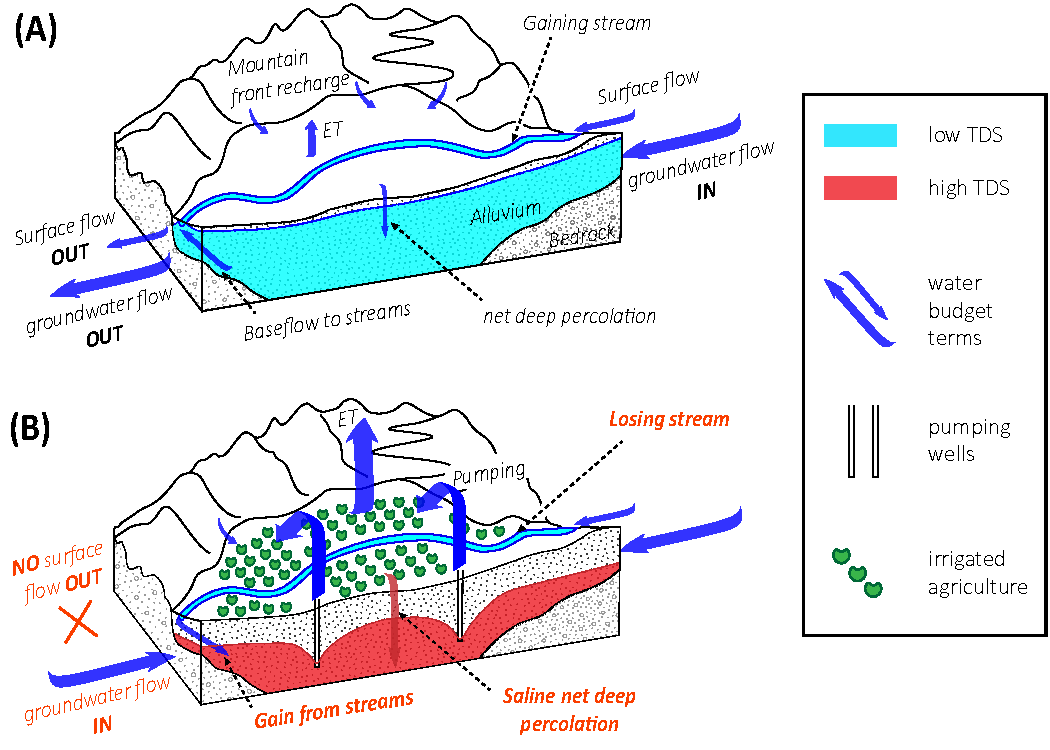
\includegraphics[width=\textwidth]{ch3_figs/mm_conceptual_model_gw_sal_2_stages.pdf}
	\caption{Conceptual model of ABCSAL. (A) Open basin, pre-groundwater development: surface and groundwater systems connect. Groundwater discharges dissolved solids into surface water which exits the basin. Groundwater at this stage is predominantly fresh (e.g., $<$ 1,000 mg/L). (B) Closed basin: groundwater pumping causes elimination of baseflow to streams. Lower groundwater levels cause subsurface inflow to drain adjacent basins. Pumped groundwater is concentrated by evapotranspiration (ET) when applied for irrigation. Salts migrate into the production zone of the aquifer, driven by vertical hydraulic gradients from recharge and pumping. Although these figures showtwo extremes (open and closed), partially-closed basins also exist.}
	\label{fig:conceptual_model_gw_sal}
\end{figure}


Importantly, we point out that the long-term continuous decline of groundwater storage is not a necessary condition for ABCSAL. Rather, even in basins where groundwater levels are stable and hence assumed to be free of overdraft, as long as they remain physically closed, they will salinate. Furthermore, although for simplicity we describe basins as either ``open" or ``closed", in reality, closure ranges from 0-100 \% (i.e., fully open to fully closed), and gradations of basin closure exist, which impact the rate of salinization and hence, the long-term temporal and vertical spatial salt distribution. Except for the most extremely exploited aquifers (one of which we explore in this study), many aquifers will fall somewhere between fully open to fully closed and not exactly at one extreme. 

In this research, we illustrate the development of ABCSAL in a historically open, freshwater basin using the agriculturally intensive Tulare Lake Basin (TLB) in California's southern Central Valley as a case study. Previous research in the TLB has shown evidence of salt accumulation in groundwater via simple water and salt budgets \citep{Kenneth1975}, and shallow aquifer salt accumulation from sediment dissolution processes in highly-soluble calcium and magnesium carbonates and sulfates \citep{Schoups2005}. Other studies have shown that TDS concentrations in TLB groundwater have increased over the last century \citep{Hansen2018, Lindsey2018}, and suggested this is the result of pumping for municipal and irrigation supply which has caused shallow, higher TDS groundwater to be driven downward into deeper aquifers. We are not aware of prior work that has placed these trends into the context of ABCSAL, or quantified potential rates of salinization across a range of aquifer depths and timescales. 

Our aim in this study is to assess the first order salt balance and timescales over which the TLB as a large production aquifer system becomes regionally degraded over most of the vertical extent of its nearly 200 $m$ thick main production zone. We conservatively assume that, under recent state regulation, groundwater overdraft is arrested, but not reversed. We compare timescales of ABCSAL degradation against the estimated lifespan of the greater Central Valley aquifer (i.e., 390 years at historical overdraft rates) \citep{Faunted.2009}, challenge the notion that the depletion of groundwater storage is a more urgent issue than the degradation of groundwater quality in the TLB (and in other basins with ABCSAL conditions), and consider the water management implications and the steps required to reverse extensive basin-scale groundwater salinization. The management would likely involve both hydrologic opening of the basin to provide natural outlets for salt, a reduction of sources of salinity, and the development of regional groundwater quality management models \citep{Fogg2006, CRWQCB2018}. The adaptation might involve the eventual desalination of most groundwater pumped from the basin, producing a future economic burden that should be anticipated and evaluated, as it bears on the security of water, food, and energy resources. 

This paper is organized as follows: first, we describe the hydrogeology, water budget, and water quality of the study site. Then we describe and justify our approach involving a simple 1D mixing cell solute transport model. Next, we present our results, and finally, we discuss the implications of the research, the limitations of our approach, and the extensibility of the study to other areas.  


%--------------------------------------------------------%
% Methods
%--------------------------------------------------------%
\section{Methods}

\subsection{Study area}
\label{ss_2_1}

In selecting the TLB as our study site, we looked for (1) a history of intensive groundwater pumping and irrigation, (2) availability of historical water budget and water quality data, and (3) social and economic significance. The TLB (Figure \ref{fig:tb_study_site}) occupies the southern third of the Central Valley, California and is bounded by the Coast Ranges to the west, the Tehachapi Mountains to the south, and the southern Sierra Nevada to the east. Geology strongly influences dissolved solid concentrations in the clastic sedimentary aquifer system composed of fluvial and alluvial fan deposits. Calcium and magnesium sulfates and carbonates in Coast Range sediment in the western TLB are more soluble than sediments from the predominately crystalline rocks of the Sierra Nevada to the east, thus the groundwater in the western basin tends to have higher TDS \citep{Fujii1995, belitz1990, deverel1988}. Fresh groundwater in the TLB spans depths from land surface to around 1,000 $m$ where brackish water and marine deposits limit the development of groundwater resources \citep{Program2010, Kang2016}. Above this deep brackish zone is a major freshwater aquifer system. In combination with a natural endowment of significant, but intermittent runoff from surrounding uplands, abundant fresh groundwater has transformed the TLB into one of the most heavily irrigated and economically productive agricultural regions in the world \citep{Hanak2011}. At its peak in the 1980s, approximately 14,164 $km^2$ of its 44,110 $km^2$ were irrigated \citep{TNC2014}. Today roughly 12,140 $km^2$ remain irrigated, with a total gross value of all agricultural crops and products at \$23.4 billion USD in 2017 \citep{kern2018, kings2018, fresno2018, tulare2018}. \\

% F:\Box Sync\Research\Post QE Research\DISSERTATION\01_mm\code\tb_study_site\tb_map.R
% tb_with_riv.pdf
% 01_mm\ai\study_site_water_budget.ai
% numbers come from archived (commented out Table 5)

\begin{figure}[H]
	\centering
	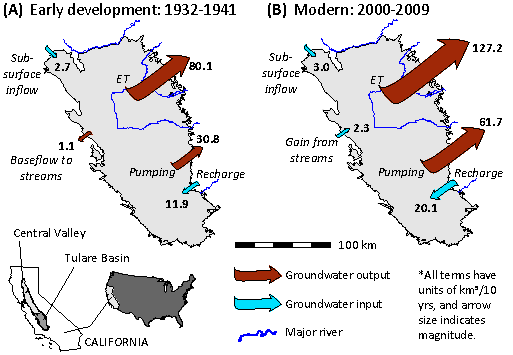
\includegraphics[width=.7\textwidth]{ch3_figs/study_site_water_budget_riv.pdf}
	\caption{The TLB overlies an agriculturally intensive sedimentary aquifer in California's southern Central Valley. Significant changes are observed in selected decadal hydrologic year water budget terms derived from C2VSim at (A) early-groundwater-development (not to be confused with pre-groundwater-development) and (B) post-groundwater-development timescales in the TLB. Notably, gaining streams transition to losing streams, and increases are observed in pumping, evapotranspiration (ET), and recharge (from diversions and natural sources, like streams, lakes, and watersheds). All terms are aggregated at the scale of the TLB, except for subsurface inflow, which is calculated at the northern TLB boundary. Note that this is not the TLB groundwater budget (Table \ref{tab_gwb}) nor the land surface and rootzone budget (SI Appendix Table \ref{ap_b_lsb}), but rather, a combination of ground and surface water budget terms that illustrate hydrologic change and show the main inputs (recharge) and outputs (pumping and evapotranspiration). Major rivers (shown in blue) from north to south include the San Joaquin, Kings, Kaweah, Tule, and Kern. Minor streams and tributaries are not shown.}
	\label{fig:tb_study_site}
\end{figure}

Although a TLB water budget from pre-development times is not available, the surface and subsurface hydrologic characteristics of the basin, which is a part of the larger Central Valley sedimentary basin (Figure \ref{fig:tb_study_site}), indicate that it was hydrologically open. We first discuss the surface hydrologic aspects. Despite the shallow topographic depression in which Tulare Lake used to exist, the freshwater lake periodically filled up and overflowed northward into the San Joaquin River \citep{grunsky1898irrigation, Davis1959}, providing an outlet for any accumulated salts. Reconstructions of historical Tulare Lake level indicate that in 19 of the 29 years from 1850 to 1878, it filled up and flowed out of the basin to the north \citep{USBR1970}. This water and salt exit via intermittent surface inundation would be different than, say, baseflow to a stream, but would accomplish the same flushing function. No overflows are documented after 1878 due to the diversion of tributary waters for agricultural irrigation and municipal water use \citep{ecorp2007}. 


\bgroup
\setlength{\tabcolsep}{1.3em}

% 01_mm_plots_tables.R in F:/ ... POst_QE_Research/DISSERTATION/01_mm
% average annual GW budget table - 1961-10-31 to 2001-09-30
% but a lot is added in the caption and table footnote, so beware changing this!!
% in MCMM.R:
% mg_to_metric_tons(sum(annual_fluxes$mass_flux[n]))/1e6, where n = the term desired

\centering
\begin{threeparttable}
	\begin{table}[H]
		\caption{Average annual groundwater and salt budget for the TLB (equation \ref{eq: gw_budget}) from C2VSim (1961-10-31 to 2001-09-30), and the modified no-overdraft budget used in this analysis (equation \ref{eq: gw_budget_mod}).}
	
		\begin{tabular}{rlrrrr}
			\label{tab_gwb}
			
			
			
			& \textbf{Source} & $\bm{Q \: \: (km^3/yr)}$ & $\bm{C \: \: (mg/L)}$ & $\bm{m \: \: (Metric \: Mtons)}$ & \\ 
			\hline
			\parbox[t]{2mm}{\multirow{8}{*}{\rotatebox[origin=c]{90}{\textbf{Historical budget}}}}
			& $R$ & 2.451 & 32.5 & 8.027E-02 & \\
			& $B$ & 0.236 & 32.5 & 7.475E-03 \\ 
			& $C$ & 0.572 & 32.5 & 1.852E-02 \\ 
			& $I$ & 0.011 & 32.5 & 3.250E-04 \\ 
			& $P$ & -6.761 & * & * \\ 
			& $N$ & 1.883 & * & * \\ 
			& $RWI$ & - & - & * & \\ 
			& $\Delta S$ & -1.608 &  &  \\ 
			
			\hline
			
			\parbox[t]{2mm}{\multirow{9}{*}{\rotatebox[origin=c]{90}{\textbf{Alternate budget}}}}
			& $R$ & 2.451 & 32.5 & 8.027E-02 & \\ 
			& $B$ & 0.236 & 32.5 & 7.475E-03 & \\ 
			& $C_{alt}$ & 0 & - & - & \\
			& $M$ & 0.678 & 32.5 & 2.204E-02 & \\ 
			& $I$ & 0.011 & 32.5 & 3.250E-04 & \\ 
			& $P_{alt}$ & -5.259 & * & * & \\ 
			& $N$ & 1.883 & * & * & \\ 
			& $RWI$ & - & - & * & \\ 
			& $\Delta S_{alt}$ & 0 & - & - & \\ 
			\hline
			\multicolumn{4}{l}{\scriptsize{* non-constant term calculated at each time step}} 
		\end{tabular}
		
		
		$Q$ is the volumetric flow rate, $C$ is the concentration of TDS, and $m$ is the mass of salt. Groundwater budget terms are:
		%$W$ = stream gain, 
		$R$ = recharge from streams, lakes, and watersheds, 
		%$L$ = lake gain,
		$B$ = lateral mountain front recharge from streams and watersheds,
		$C$ = subsidence flow,
		$C_{alt}$ = subsidence flow to eliminate overdraft (along with $M_{alt}$ and $P_{alt}$),
		$M$ = managed aquifer recharge to eliminate overdraft (along with $C_{alt}$ and $P_{alt}$), 
		$I$ = subsurface inflow from the north,
		$P$ = groundwater pumping,
		$P_{alt}$ = alternate groundwater pumping to eliminate overdraft (along with $M$ and $C_{alt}$),
		$N$ = net deep percolation (recharge from the land surface through vadose zone and into saturated groundwater),
		$RWI$ are rock-water interactions.
		$\Delta S$ = change in groundwater storage.
		$\Delta S_{alt}$ = change in groundwater storage for the modified budget. 
		The modified budget eliminates overdraft by reducing $P$ to $P_{alt}$ according to equation (\ref{eq: pumping_in_cells}), and introducing recharge $M$. 
		
	\end{table}
	
\end{threeparttable}

\egroup

\clearpage


The subsurface characteristics also indicate open hydrologic conditions. There is significant evidence that groundwater flowed northward into the adajacent San Joaquin Basin in pre-development times (circa early 1900s). This evidence includes (1) historical measurements of Central Valley groundwater TDS showing lowest TDS values in the TLB, with increasing TDS to the north into the San Joaquin Basin \citep[Table 23]{mendenhall1916ground}, consistent with northward groundwater flow and the accompanying down-hydraulic-gradient groundwater chemistry evolution that is routinely observed in sedimentary basins, e.g., \citep{palmer1984geochemical}; (2) the regional, south-to-north topographic gradient to provide the driving force for gravity-driven flow in the same direction, out of the TLB, even if there existed shallower, local groundwater flow components from north to south at the subtle depression that collected Tulare Lake (e.g., refer to classic work of \cite{toth1970conceptual} on topographically controlled, gravity-driven flow systems); and (3) horizontal stratification of fine- and coarse-textured sediments in the Central Valley sedimentary basin that results in much lower effective hydraulic conductivities in the vertical direction than the horizontal e.g., \citep{weissmann2002dispersion, Faunted.2009}, thereby minimizing influence of subtle topographic features like the Tulare Lake depression on all but the shallowest groundwater flow components (e.g., refer to \cite{toth1970conceptual} and related work).

Summarizing, our conceptual model of the pre-development TLB hydrologic system is one in which the subtle topographic depression that collected the typically 12 $m$ deep Tulare Lake \citep{preston1990tulare}, together with the periodic overflow of the lake and discharge to the north, resulted in a partly open surface drainage system. Further, the larger topographic and geologic structure of the basin, together with groundwater chemistry evidence, indicates there was net-northward groundwater flow, making the TLB groundwater system an open hydrologic basin in pre-development times.

Parts of TLB may have been salinating to some degree before development due to shallow evaporation of groundwater and surface water (case (3) in Introduction), in contrast to the ABCSAL process that we describe in this paper. Portions of the TLB closed under pre-development conditions would lead to salt accumulation in and near its playas (e.g., Buena Vista Lake, Tulare Lake): an evaporative boundary of the basin and endpoint to all surface water discharge (case (2) above). This is consistent with observations of high salinity near and in these lakebeds \citep{Hansen2018, Fujii1995}. Although there exist local areas of shallow groundwater with elevated salinity on the west side of the TLB, these areas are typically associated with salt mobilization out of alluvial sediments originating from marine sedimentary source rocks in the Coast Ranges, and not from basin closure.

By the time regional groundwater levels were mapped in the early twentieth century, the TLB showed signs of closure: groundwater flow across the northern boundary was minimal, and flowed north to south, into the TLB \citep{mendenhall1916ground, ingerson1941hydrology}. Although pre-groundwater-development (pre-1850) water budgets are unavailable, two large-scale, regional groundwater flow models of the Central Valley \citep{Brush2013, Faunted.2009} provide decadal groundwater budgets for early- (1932-1941) and post-groundwater-development (2000-2009) timescales.

Relative to the decadal hydrologic water year budgets of early-groundwater-development, post-groundwater-development water budgets show much higher pumping, crop evapotranspiration, and recharge \citep{Brush2013}. As groundwater levels fell, gaining streams transitioned to losing streams, and subsurface inflow along the northern basin boundary slightly increased (Figure \ref{fig:tb_study_site}). Groundwater discharge to surface water almost entirely ceased. Surface water exits the basin in rare years when the Kings, Kaweah, and Kern rivers produce sufficiently large floods, mostly runoff from the surrounding uplands. Evapotranspiration from irrigated crops has become the dominant water outflow, and this flow is much greater than it was during early-groundwater-development \citep{Brush2013}. Taken together, these hydrologic changes have transitioned the TLB into an anthropogenically closed groundwater system with commensurate onset of ABCSAL.  




%
%---------------- MODEL DEVELOPMENT ------------------%
%
\subsection{Mixing Cell Model Development}
\label{ss_2_3}

Given the large space and time scales of interest, and the large-scale effectively one-dimensional vertical flow conditions in the basin due to pumping and recharge, we used a lumped parameter approach based on upscaling water fluxes of a fully three-dimensional groundwater model. % was employed as an appropriately parsimonious modeling tool. 
Although local hydrogeologic conditions vary and can lead to locally complex three-dimensional flow and transport, our focus here is on large scale salinization behavior and time scales, thus an upscaled model was appropriately parsimonious. %which is well-captured with a one-dimensional approach. %We assess results against existing fully three-dimensional flow and salt transport models that also address aquifer heterogeneity, albeit at spatial scales significantly smaller than the TLB, to ascertain the appropriateness of the mixing cell approach chosen here.
Moreover, upscaling the advection dispersion equation to regional scales remains a scientific and computing challenge \citep{guo2019adaptive, guo2019upscaling} beyond the scope of this study.

Mixing cell models, also called discrete-state compartment models, are computationally inexpensive and have successfully been used in place of complex flow models to provide rapid, first-order estimates of water budgets, mass flux, and contaminant concentrations \citep{Campana1975, Campana1984, Campana1987, Carroll2008, Kirk1990}. A mixing cell approach segments the system into a set of control volumes. In each time step of the model, water and salt masses are passed between the cells, and new concentrations are calculated at each cell. Here, we represent the TLB groundwater system through a one-dimensional, vertical column of discrete control volumes (cells), given the predominance of vertical downward flow at the aquifer system scale. We assume that each cell consists of a fraction $f$ of sediments participating in groundwater flow and salt transport with porosity $\eta$. We neglect flows and rock-water interactions in sediments not participating in transport, of proportion $1-f$ (more details below). The thickness of each cell is chosen such that the advective travel time ($\Delta t$) of water and salt downward through each cell is exactly 50 years (synchronized tipping bucket model, see equation \ref{eq: discretization}) below, thus full mixing occurs at each cell even as the groundwater flow velocity decreases with depth. To determine the mixing cell parameters, water fluxes throughout the vertical domain (e.g., recharge, vertical flow rate, pumping) are obtained by averaging (i.e., mass-conservative upscaling) the TLB portion of a fully three-dimensional, heterogeneous groundwater flow model of the Central Valley \citep{Brush2013}.  

The salt accumulation in a mixing cell at a discrete time $k$ is a mass balance of the initial mass ($m_k$) $[M]$, incoming mass ($m_k^{in}$) and exiting mass ($m_k^{out}$).  

\begin{equation}
m_{k+1} = m_k + m_k^{in} - m_k^{out}
\label{eq: mass_balance}
\end{equation}  

Input and output mass terms can be calculated for each term in the water and salt budget (Table \ref{tab_gwb}), from their input and output concentration ($C_k^{in}$, $C_k^{out}$ $[ML^{-3}]$) and input and output volumetric flow ($Q_k^{in}$, $Q_k^{out}$ $[L^3]$):

\begin{equation}
m_k^{in} = C_k^{in} Q_k^{in}   \: \: ; \: \:  m_k^{out} = C_k^{out} Q_k^{out}
\label{eq: m_in_cell}
\end{equation}

Finally, the concentration in a mixing cell at time step $k$ is:

\begin{equation}
C_{k+1} = \frac{m_k + m_k^{in} - m_k^{out} + \rho V}{V f \eta}
\label{eq: c_in_cell}
\end{equation}


where $V$ $[L^3]$ is the total cell volume, $f$ $[-]$ is the fraction of sediments actively participating in groundwater flow and salt transport, $\eta$ $[-]$ is the porosity of those sediments, and $\rho$ $[ML^{-3}]$ is rock-water interaction coefficient. The fraction $f$ is found to be 0.99 \citep{Brush2013}, which in the C2VSim model includes all textures but the Corcoran clay, a relatively impermeable clay layer comprising around 1\% of the model volume. Porosity, $\eta$, is set to 0.40, the average for the TLB. Coarse and fine sediment porosities do not appreciably differ, averaging around 0.40 with an interquartile range of 0.39 - 0.41 for all textures, as demonstrated in abundant core analyses \citep{Johnson1968}, and discussed further in SI Appendix Table \ref{ap_b_porosity_boot} and Figure \ref{ap_b_porosity_boot_hist}; hence, we did not consider varying $\eta$ across aquifer layers. 

To account for mass contribution from natural dissolution of geologic minerals, we define a zero order source term called the rock-water interaction coefficient $\rho$ $[ML^{-3}]$. Rock dissolution along groundwater flow paths is well documented in sedimentary aquifers \citep{palmer1984geochemical, oetting1996regional, toth1999groundwater, mahlknecht2004groundwater, cloutier2008multivariate}. We obtain a representative mass dissolution rate from the slope of a representative TDS profile for the TLB from land surface to the base of fresh water \citep{Williamson1989, Kang2016}. The product of the rock-water interaction coefficient $\rho$ and the cell volume ($V$) is the additional mass accumulated from rock-water interactions in the cell. We also evaluate an alternative scenario with $\rho =$ 0. 

We solve (\ref{eq: c_in_cell}) sequentially over the stacked mixing cells from top to bottom and across seven 50-year time steps from 1960 (initial condition) to 2310 (synchronized tipping bucket approach) to obtain the variation of salinity with depth and time. 

The discretization, $\Delta z_j$, of the stacked series of mixing cells (Figure \ref{fig:conceptual_model_mm}) is driven by the time step, $\Delta t$ = 50 years, and the representative basin-scale vertical Darcy velocity, $q_j$, within the $j^{th}$ mixing cell:

\begin{equation}
\Delta z_j =  \frac{q_j}{f \eta}  \cdot  \Delta t
\label{eq: discretization}
\end{equation}

Since $q_j$ is depth dependent, we solve (\ref{eq: discretization}) sequentially for $j$ = 1...m, beginning at the water table to compute the vertical discretization of the stacked mixing cell model. Here, we assume that the inflow into a mixing cell, $q_{j-1, j}$ is representative of the flow rate $q_j$ throughout the cell. Thus -- to compute cell thicknesses with equation (\ref{eq: discretization}) -- the pumping, $P_j$, lateral basin flow $I_j$, or subsidence flow $C_j$ (Figure \ref{fig:conceptual_model_mm}) conceptually flow into or out of the mixing cell bottom. The following sections provide further details on the parametrization of (\ref{eq: c_in_cell}) and (\ref{eq: discretization}).

\begin{figure}[H]
	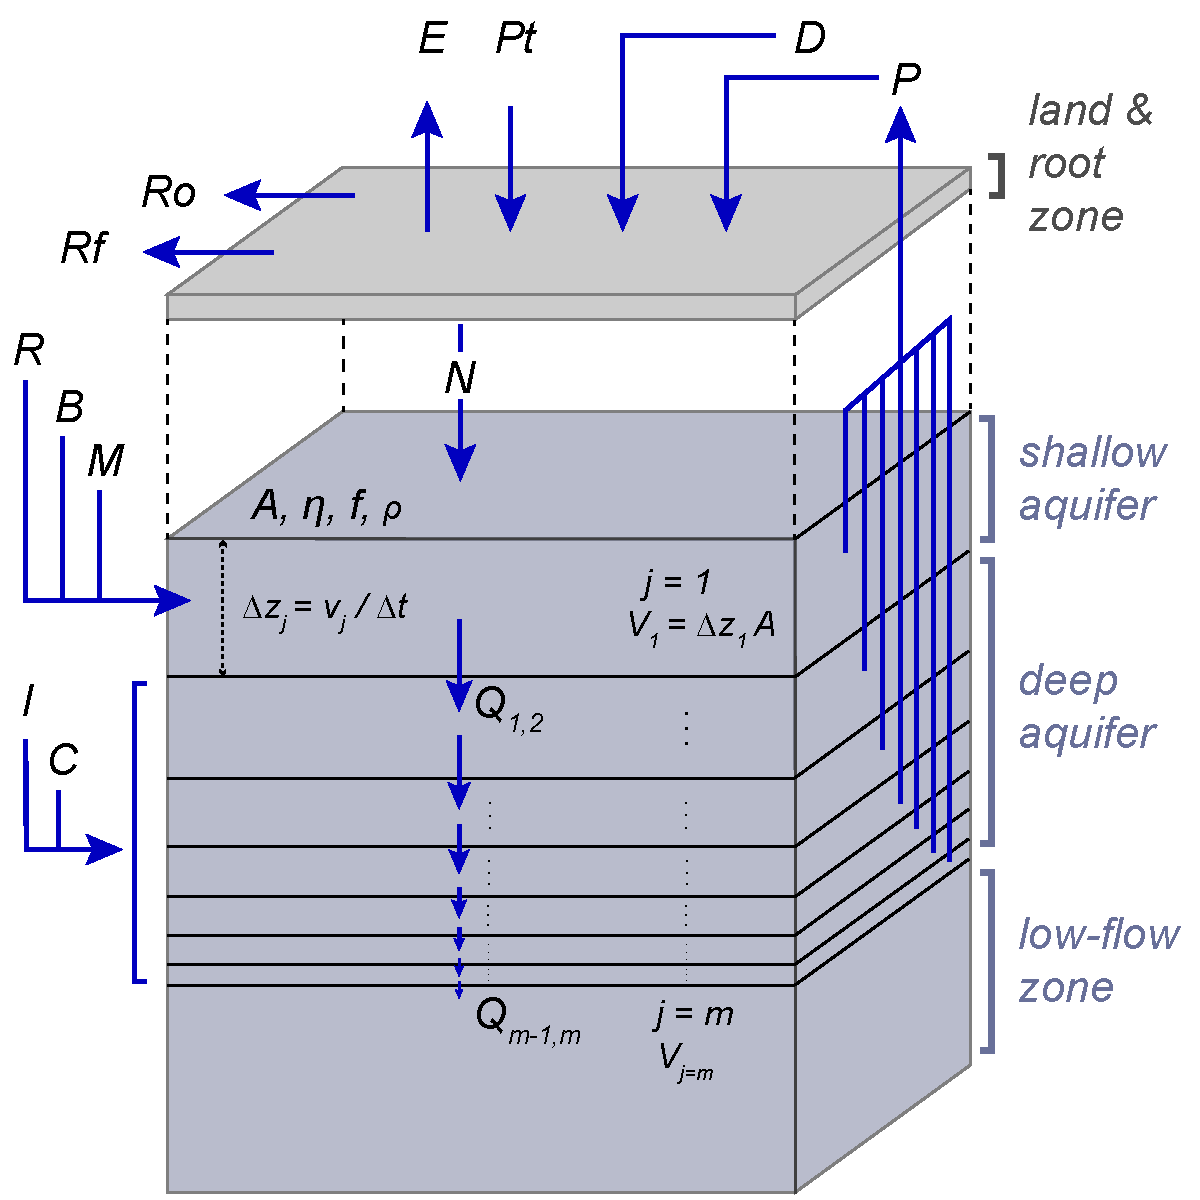
\includegraphics[width=\textwidth]{ch3_figs/mm_conceptual_model.pdf}
	\caption{Conceptual land-rootzone model and groundwater mixing cell model with surface area $A$, porosity $\eta$, aquifer fraction $f$, rock-water interaction coefficient $\rho$, and $m$ cells. The cell thickness $\Delta z_j$ is given per equation (\ref{eq: discretization}), where average linear velocity $v_j$ = $q_j / f \eta$. The cell volume $V_j$ is the total bulk volume of the rock including aquifer and non-aquifer material. The TDS in cell $j$ is calculated by equation (\ref{eq: c_in_cell}). The land and root budget (SI Appendix Table \ref{ap_b_lsb}) accounts for pumping ($P$), surface water diversions ($D$), precipitation ($Pt$), evapotranspiration ($E$), runoff ($Ro$), return flow ($Rf$), and net deep percolation ($N$). $N$ enters the top of the groundwater mixing cell model along with recharge from streams, lakes, and watersheds ($R$), boundary inflow from mountain front recharge ($B$), and managed aquifer recharge ($M$). Internal flows from subsurface inflow from the north ($I$), subsidence flow ($C$), and pumping ($P$) are distributed proportional to cell volume, e.g., equation (\ref{eq: pumping_in_cells}). The average annual groundwater and salt budget is reported in Table \ref{tab_gwb}.}
	\label{fig:conceptual_model_mm}
\end{figure}



%
%---------------- BOUNDARY CONDITIONS ------------------%
%
\subsection{Boundary conditions, model parameters, and stochastic simulation}
\label{ss_2_4}

Initial conditions, boundary conditions, and model parameters are informed by the C2VSim groundwater flow model developed by the California Department of Water Resources \citep{Brush2013}, publicly available water quality data \citep{CSWRCB}, and previous field studies of the TLB. The following describes methods used to determine (1) water and salt budgets, (2) salt fluxes from evaporative concentration and pumped groundwater, (3) the groundwater velocity-depth profile, (4) the initial TDS-depth profile, and (5) spatial parameters and aquifer properties. Lastly, we discuss the simulation timescale and the role of stochastic simulation.

%
%---------------- SALT/WATER BUDGETS ------------------%
%
\subsubsection{Water and salt budgets}
\label{ss_2_5}

The water budget is based on C2VSim version 3.02, a 3 layer and 1,392 element, regional scale, finite-element groundwater flow model of California's Central Valley alluvial aquifer system \citep{Brush2013}. C2VSim is an application of the Integrated Water Flow Model (IWFM) \citep{Dogrul2018}, a water resources management and planning model that simulates surface water, stream-groundwater interaction, vadose zone flow, and groundwater flow. In the C2VSim model, California's Central Valley aquifer is separated into 21 subregions, and detailed land surface, root zone, and groundwater budgets for each subregion are calculated at monthly time steps from the 1923 to 2009 hydrologic years. The TLB is represented by subregions 14-21. Because of its detailed representation of surface-groundwater interaction, groundwater pumping, three-dimensional aquifer structure, and calibration, C2VSim was chosen as a reasonable representation of the TLB water budgets, groundwater velocities, and thus chosen to develop the mixing cell model. 

The C2VSim model was run for the 40-year period from 1961-10-31 to 2001-09-30 to obtain an average annual TLB groundwater budget (an equivalent average annual landscape/root zone budget is provided in SI Appendix Table \ref{ap_b_lsb}). This post-groundwater development water management time frame is characterized by pumping and overdraft, in addition to wet, dry, above normal, below normal, and critical water year types. The C2VSim change in groundwater storage is defined as:

\begin{equation}
\Delta S = R + B + C + I + N - P
\label{eq: gw_budget}
\end{equation}

where $\Delta S$ is change in groundwater storage [$L^3$], $R$ is basin recharge from streams, lakes, and watersheds [$L^3$], $B$ is lateral mountain front recharge from streams and watersheds [$L^3$], $C$ is subsidence based flow from clay compaction [$L^3$], $I$ is subsurface inflow from the north [$L^3$], $N$ is net deep percolation predominately from irrigation water [$L^3$], and $P$ is groundwater pumping [$L^3$]. The dominant budget terms are $P$, $R$, and $N$ (Table \ref{tab_gwb}). 

To demonstrate ABCSAL under long-term conditions that avoid further overdraft (but not basin closure), we solve the mixing cell model equations (\ref{eq: c_in_cell}) - (\ref{eq: discretization}) alternatively for $\Delta S_{alt}$ = $\Delta C_{alt}$ = 0. Overdraft is eliminated with an alternate budget (Table \ref{tab_gwb}), which adds managed aquifer recharge, $M$ as inflow to the top mixing cell (Figure \ref{fig:conceptual_model_mm}), and reduces pumping to an alternative pumping level, $P_{alt}$. We add $M$ = 0.68 $km^3$, which was determined by a prior study as the maximum theoretical recharge available to the San Joaquin Valley (which includes the TLB), assuming unlimited infrastructure and water transfer ability \citep{Hanak2019}. Eliminating overdraft in this way effectively maintains a steady-state, saturated model that remains closed to due to lack of baseflow and groundwater outflow. Hence, the water level is immobile, but the salt front can move, thus simulating salt migration without drying out cells due to overdraft.

Since $M$ represents captured surface water flow, we assign it the same TDS as natural water (32.5 $mg/L$), discussed below. We also simulated $M$ with a TDS of 0 $mg/L$ (SI Appendix Table \ref{ap_b_p_sim_m_with_tds_0}
) and found that it had a negligible impact on resulting salt concentrations presented in this study (SI Appendix Table \ref{ap_b_p_sim}). 

The alternate, reduced pumping $P_{alt}$, is computed by rearranging (\ref{eq: gw_budget}), adding $M$, and setting $\Delta S_{alt}$ = $C_{alt}$ = 0:

\begin{equation}
P_{alt} = R + B + M + I + N 
\label{eq: p_alt}
\end{equation}

%[THE FOLLOWING ONLY IF YOU WERE TO USE YOUR CURRENT RESULTS FROM 2010 AS INITIAL CONDITIONS FOR YOUR RUNS USING (6) FOR THE PERIOD FROM 2010 to 2265:]
%We use (5) to simulate the historic period 1960-2010, and the resulting concentration profile as initial condition for using (6) to solve for flow and transport conditions from 2010 - 2265.

Therefore, the modified no-overdraft alternate groundwater budget is:  

\begin{equation}
\Delta S_{alt} = R + B + C_{alt} + M + I + N - P_{alt} = 0
\label{eq: gw_budget_mod}
\end{equation}


The salt budget is calculated by assigning a TDS concentration to each term in the groundwater budget (\ref{eq: gw_budget_mod}). TDS for natural waters (e.g., stream, lake, and managed aquifer recharge budget terms) were determined to be 32.5 $mg/L$, by computing the median of the sampling distribution of sample TDS medians in TLB stream samples \citep{nwis} from 1951 - 2019 (SI Appendix Figure \ref{ap_b_nat_waters} and Table \ref{ap_b_gw_and_sw_c_summary}). Similarly, the TDS of diverted surface water was calculated to be 264.5 $mg/L$, as the average annual water and salt budget from 1985 - 1994 of two major surface water conveyance structures, the California State Water Project and the State Water Project \citep{Cismowski2006} (SI Appendix Table \ref{ap_b_gw_and_sw_c_summary}). Salt and water budgets are detailed in Table \ref{tab_gwb}. 


%
%---------------- VELOCITY DEPTH PROFILE ------------------%
%
\subsubsection{Velocity-depth profile}
\label{ss_2_6}

To explicitly solve for the mixing cell discretization (\ref{eq: discretization}), we fit a linear model to the C2VSim vertical Darcy velocities, reported for each finite element cell in the three layer C2VSim grid at the layer-to-layer boundaries. Due to increases in recharge and pumping caused by groundwater development and irrigation, the groundwater flow system is vertically dominant, and thus supports the application of a 1D, vertically oriented model. To account for groundwater velocity change in the alternate groundwater budget (\ref{eq: gw_budget_mod}), groundwater velocity is scaled proportional to the decrease in vertical volumetric flow rate, $P_{alt}/(P + C)$ = 0.85 (a 15 \% reduction). This is equivalent to the ratio of net downward volumetric flow in the alternate budget to the net downward volumetric flow in the historical budget (Table \ref{tab_gwb}). 

\begin{equation}
q(z) = (\beta_0 + \beta_1 z) \cdot \frac{P_{alt}}{P+C}
\label{eq: vel}
\end{equation}

where $\beta_0$ and $\beta_1$ are the regression coefficients (SI Appendix Table \ref{ap_b_velocity_coefficients}), and the overall change (reduction) in velocity is -15\%. Mixing cell thickness (\ref{eq: discretization}) is determined by computing $q_j$ from (\ref{eq: vel}) for the depth, $z$, of the bottom of the mixing cell $j-1$ (top of cell $j$). To ensure consistency between the water balance terms in (\ref{eq: gw_budget}) and the approximated vertical velocity profile (\ref{eq: vel}), we compute the water mass balance error, $MB_{error, j}$, for each mixing cell $j$:

\begin{equation}
MB_{error, j} = q_{j-1,j} + I_j - P_{alt,j} - q_{j,j+1}
\label{eq: mb_error_inside}
\end{equation}

For the uppermost mixing cell $j$ = 1, we rearrange (\ref{eq: mb_error_inside}), replacing $q_{j-1,j}$ for the sum of $N$, $R$ and $B$, and ignoring subsurface inflow $I_j$ (Figure \ref{fig:conceptual_model_mm}):

\begin{equation}
MB_{error, 1} = N + R + B + M - P_{alt,1} - q_{1,2}
\label{eq: mb_error_top}
\end{equation}

The cell by cell budget and mass balance errors (which are effectively zero, and equivalent to the cell-by-cell change in storage) are reported in SI Appendix Table \ref{ap_b_cbc}.


%
%---------------- EVAPOCONCENTRATION ------------------%
%
\subsubsection{Evapoconcentration and pumping}
\label{ss_2_7}

Evapotranspiration removes a majority of total applied water, leaving behind dissolved solids in the crop rootzone that eventually migrate into groundwater. We model the evapoconcentration of TDS in total applied water (a combination of pumped groundwater and imported surface water diversions) by accounting for the application efficiency \citep{burt1997irrigation}, and thus the fraction of water that remains after evapotranspiration:  

\begin{equation}
C_N = \left( \frac{m_D + m_P}{V_D + V_P} \cdot \frac{1}{1 - E_a} \right) = \frac{C_{D,P}}{1 - E_a}
\end{equation}

$C_N$ is the concentration of net deep percolation after accounting for evapotranspiration. $m_D$ and $m_P$ are the mass, and $V_D$ and $V_P$ are the volume of surface water diversions ($D$) and pumping ($P$), respectively. $C_{D,P}$ is the concentration of total applied water from surface water diversions and pumping (calculated by mixing diversions and pumped groundwater in their respective proportions, see SI Appendix Table \ref{ap_b_velocity_coefficients}), and $E_a$ is the application efficiency, which has a measured regional average of 0.78 in the Tulare Basin \citep{sandoval2013spatial}, and agrees with measured values in hydrologically similar areas \citep{hanson1995, howell2003irrigation}. Alternatively, the C2VSim landscape/soil water budget (SI Appendix Table \ref{ap_b_lsb}) provides an application efficiency, $E_a$, of 0.88 when considering the amount of water infiltrating into the soil and deep percolation. For sensitivity analysis, we run simulations for several $E_a$ between 0.78 and 0.88 to further explore model outcome uncertainty.

For the stacked mixing cell model, we assume that $P_{alt}$ in the no-overdraft groundwater budget (\ref{eq: p_alt}) is distributed uniformly with depth, from the water table to the last mixing cell $m$. Similarly, we assume lateral inflow $I$ is uniformly distributed across depth, from cell 2 to cell $m$. Therefore, pumping is proportional to mixing cell thickness, and the salt mass flux due to pumping during time step $k$ in mixing cell $j$ is:

\begin{equation}
m_{j,k} = \frac{V_j f \eta}{f \eta \sum_{i=1}^{n} V_i} P C_{j,k}
\label{eq: pumping_in_cells}
\end{equation}

Noting that the $f \eta$ term drops out, and summing over all mixing cells at time $k$ gives the total mass flux from groundwater pumping ($m_{P, k}$):  

\begin{equation}
m_{P, k} = \sum_{j=1}^{n} \frac{V_j}{\sum_{i=1}^{n} V_i} P C_{j, k}
\end{equation}




%
%---------------- INITIAL CONCENTRATION ------------------%
%
\subsubsection{Initial TDS-depth profile}
\label{ss_2_8}

The initial TDS-depth profile is determined by fitting a linear model to the pre-1960 TDS-depth measurements (Figure \ref{fig:predev_tds_bc}) \citep{CSWRCB}. Due to the influence of freshwater recharge at the land surface and rock-water interactions, pre-1960 TDS generally increases with depth, consistent with observations of increasing TDS with depth in the region \citep{Kang2016, Kharaka1992, Program2010}. \\  

% in F:\Box Sync\Research\Post QE Research\DISSERTATION\01_mm\code\02_reanalyze_gw_tds.R
% search predev_tds_bc.pdf
% edited in ai/predev_tds_bc.ai
\begin{figure}[H]
	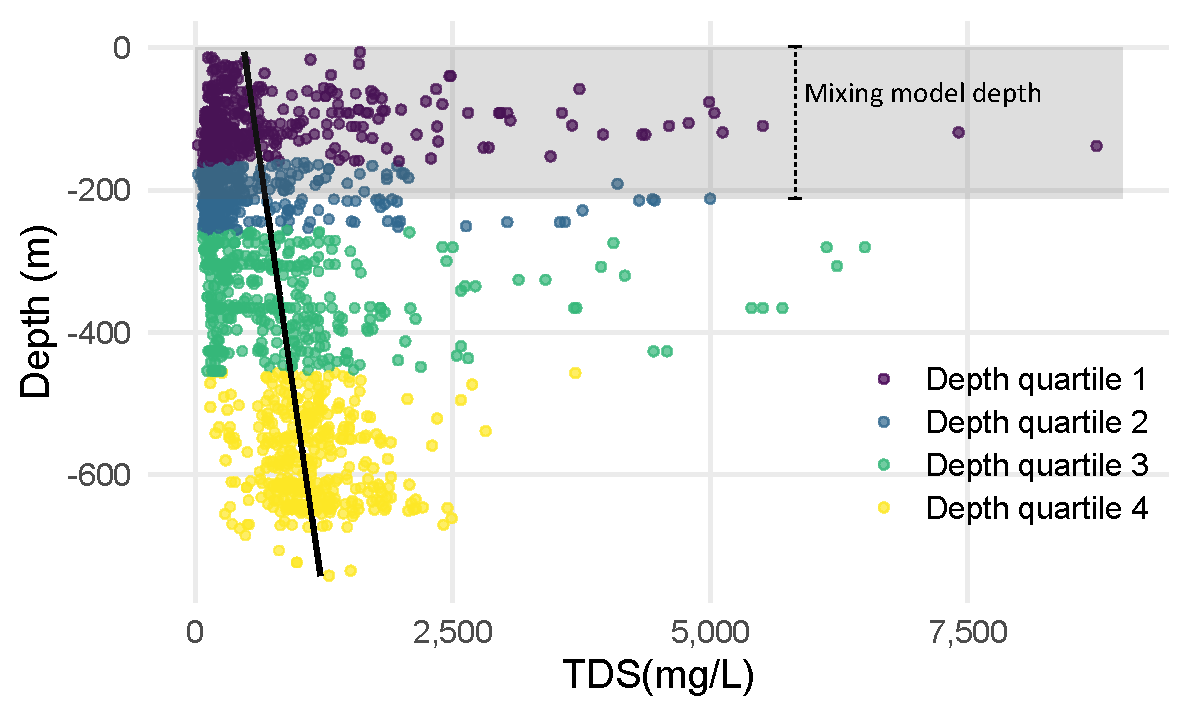
\includegraphics[width=\textwidth]{ch3_figs/predev_tds_bc.pdf}
	\caption{Pre-1960 groundwater quality generally decreases with depth, reaching an average concentration of 1,000 mg/L at 526 $m$ deep. The initial TDS-depth concentration at $t$ = 0 is approximated by a linear model, shown as a black line. The transparent, grey rectangle shows the depth of the mixing cell model (212 $m$).}
	\label{fig:predev_tds_bc}
\end{figure}


%
%-------- ENSEMBLE SIMULATION ------------%
%
\subsubsection{Ensemble simulation}
\label{ss_2_9}

We assign a uniform probability distribution to the parameters of which we are least certain and discrete values to those that are measured (SI Appendix Table \ref{ap_b_geometry}), then perform Monte Carlo simulation to generate an ensemble output. The mixing cell model is evaluated 1,000 times -- which the computational simplicity of a lumped model permits; modeling uncertainty in this way with a distributed parameter, 3D flow and transport model would be computationally prohibitive. Parameter ranges are estimated from literature for rock-water interaction coefficient \citep{Williamson1989, Kang2016}, detailed in section \ref{ss_2_3}. As described in section \ref{ss_2_7}, application efficiency is both measured \citep{sandoval2013spatial}, and calculated from C2VSim \citep{Brush2013}.  

To show the influence of rock-water interactions on the progression of closed basin salinization, we simulate two basic scenarios:  

\begin{enumerate}
	\item No rock-water interactions: mass accumulates from water budget inputs.  
	\item Rock-water interactions are present: mass accumulates from water budget inputs, but also internally via rock-water interactions (see section \ref{ss_2_3} for details).  
\end{enumerate} 




%--------------------------------------------------------%
% Results
%--------------------------------------------------------%

\section{Results}
\label{s_3}

%
%----------- GW and SALT BUDGET ---------------%
%
\subsection{Groundwater and salt budget}
\label{ss_3_1}

The average historical C2VSim groundwater budget in the TLB from 1961-10-31 to 2001-09-30 (Table \ref{tab_gwb}) reflects post-groundwater development conditions. Pumping removes an average of -6.76 $km^3/yr$ from the groundwater system. Natural recharge from streams, lakes, and watersheds adds an average of 2.45 $km^3/yr$, and net deep percolation of agricultural irrigation adds an average of 1.89 $km^3/yr$. Smaller sources of water inflow include subsidence flow (0.57 $km^3/yr$), lateral mountain front recharge from streams and watersheds (0.24 $km^3/yr$), and subsurface inflow from the north (0.01 $km^3/yr$). 

The alternate budget (Table \ref{tab_gwb}) used in this study eliminates overdraft ($\Delta S$ = 0), and is identical to historical budget described above, except that pumping $P_{alt}$ is reduced to -5.26 $km^3/yr$, managed aquifer recharge $M$ is added at a rate of 0.68 $km^3/yr$, and subsidence flow $C_{alt}$ is reduced to 0. Importantly, in this alternative budget the basin remains closed.

Salt inputs to the system (Figure \ref{fig:salt_ec}A) come from pumped groundwater, water budget terms, and rock-water interactions.


Groundwater pumping for agriculture is unlike other water budget terms ($I, M, R, B$) and rock-water interactions in that it does not \textit{add} new salt into the system, but rather \textit{recycles} existing salt from deeper layers to the land surface and back into shallow groundwater via irrigation (discussed in Section \ref{ss_3_3}). In the no rock-water interactions scenario ($\rho = $ 0), the median mass recycled by pumped groundwater exceeds the mass input of all other water budget terms by a factor of 1.7 to 3.5
% MCMM.R df5$m[c(43,49)]/(df5$m[c(36,41)] + df5$m[c(29,35)])
depending on the timeframe considered. When rock-water interactions are present ($\rho > $ 0), they initially contribute a comparable mass to groundwater pumping (around 4 metric $Mtons$), but with time, salt accumulates in the aquifer, and the mass recycled by groundwater pumping exceeds the mass imparted by rock-water interactions (Figure \ref{fig:salt_ec}A). 

Annually, surface water diversions add 1.5 
% MCMM.R   df5$m[1]/1e6
metric $Mtons$ of salt to the study site. This is around 4
% MCMM.R   (df5$m[1]/1e6 ) / (df5$m[8]/1e6)
times the amount of all other non-pumping water budget terms combined ($I, M, R, B$), which add only 0.35 
% MCMM.R   df5$m[8]/1e6
metric $Mtons$. We estimate that rock-water interactions add between 3.3 metric $Mtons$ and 4.6
% MCMM.R   c(df5$p5[22], df5$p95[28])/1e6
metric $Mtons$ of salt annually. This exceeds the mass introduced by imported surface water and is comparable to the mass recycled by groundwater pumping. 


% in Github/Monte-Carlo-Mixing-Model/code/MCMM.R
% search p23.pdf
\begin{figure}[H]
	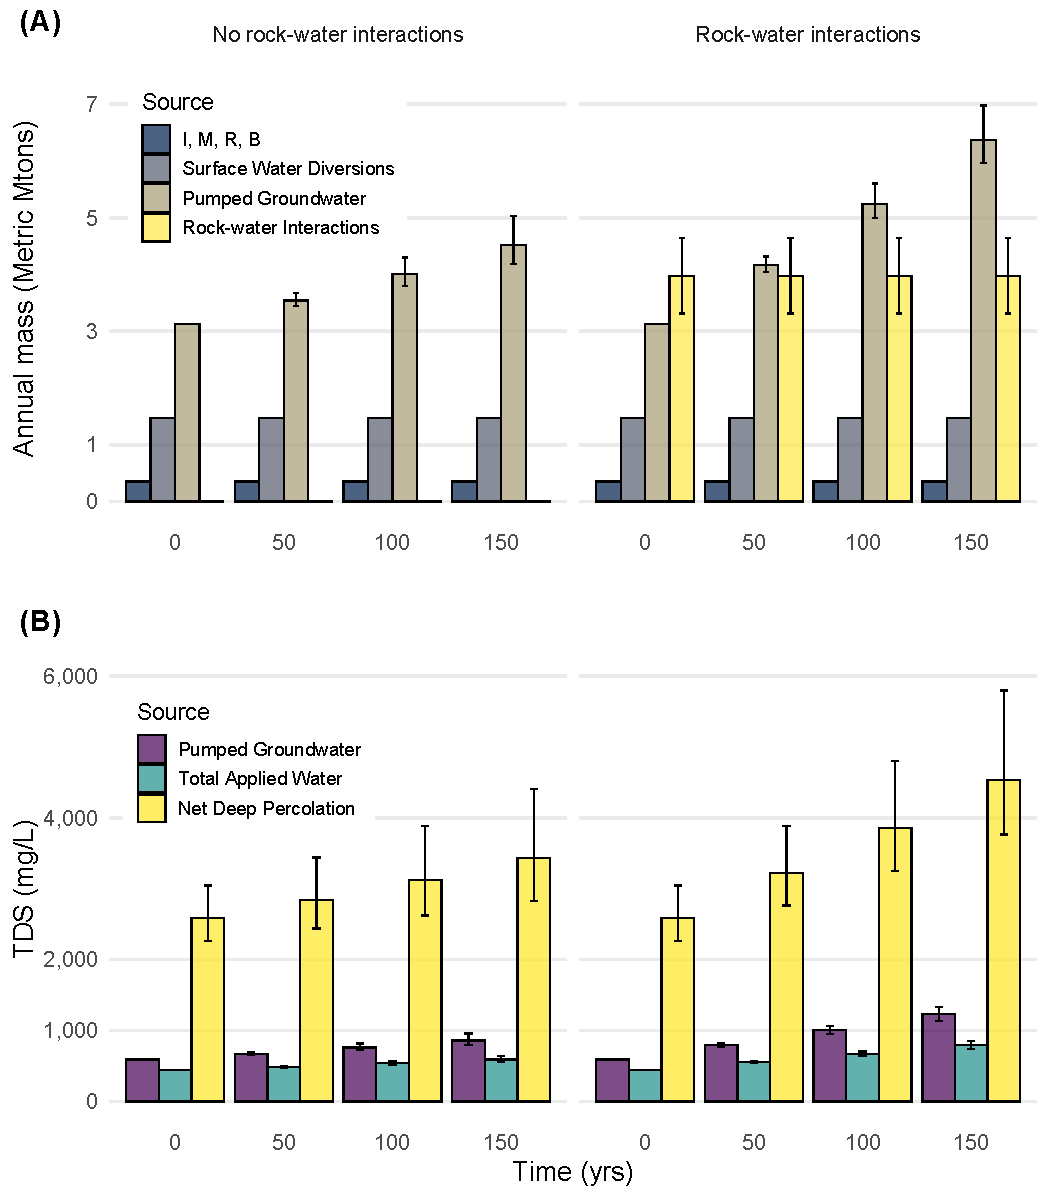
\includegraphics[width=\textwidth]{ch3_figs/p23.pdf}
	\caption{Annual mass flux and TDS of selected budget terms. The height of each column is the ensemble median result, and the width of error bars, if present, is the interquartile range of the ensemble distribution. (A) Pumped groundwater contributes more mass than surface water diversions and all other water budget terms combined (represented by their symbol: $I, W, R, B$). (B) TDS of \textit{pumped groundwater} is diluted when mixed with imported surface water, which forms \textit{total applied water}. However, evapotranspiration concentrates total applied water, which enters the groundwater system as \textit{net deep percolation}. Over time in a closed basin system, the groundwater salinates, which in turn increases the concentration of total applied water and net deep percolation. }
	\label{fig:salt_ec}
\end{figure}



Due to the closed-basin hydrology of the study site, there are no exits for salt to leave the system. Instead, pumping and irrigation recycle salts within the basin, and evapotranspiration by crops at the land surface increases the concentration of net deep percolation, which recharges groundwater (Figure \ref{fig:salt_ec}B). 

Evapoconcentration by crops at the land surface increases the average concentration of total applied water (pumped groundwater combined with surface water diversions) by 5.1 - 6.8
% (filter(EC_dat2, time == 0 & legend == "C") %>% slice(1) %>% .$p5 ) / (filter(EC_dat2,time == 0 & legend == "B") %>% slice(1) %>% .$p95 ) 
% (filter(EC_dat2, time == 0 & legend == "C") %>% slice(1) %>% .$p95 ) / (filter(EC_dat2,time == 0 & legend == "B") %>% slice(1) %>% .$p5 ) 
times its original amount, regardless of whether rock-water interactions are absent or present. As previously discussed, since pumped groundwater concentration increases with time, total applied water and thus net deep percolation also become increasingly saline over time.  




%
%----------- GW SAL EVOLUTION ---------------%
%
\subsection{Progression of groundwater salinization}
\label{ss_3_3}

The shallow aquifer (36 $m$) is heavily impacted by the recycling of salts via pumping and irrigation, and exceeds the freshwater concentration threshold (1,000 $mg/L$) within decadal timescales (Figure \ref{fig:p_sim}). Intermediate (132 $m$) and deep aquifers (187 $m$) exceed 1,000 $mg/L$ within century-long timescales. \\

% in Github/Monte-Carlo-Mixing-Model/MM_no_RWI.Rmd
% search p_sim.pdf
% edited in AI in DISSERTATION/01_mm/ai/p_sim_both2.ai
\begin{figure}[H]
	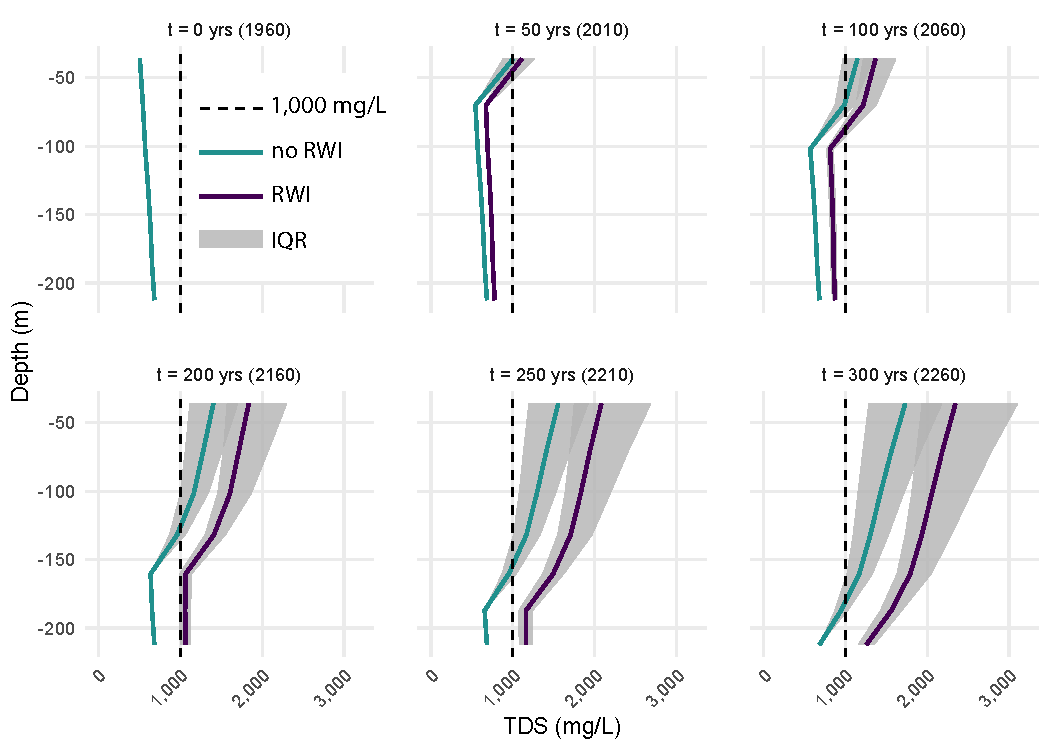
\includegraphics[width=\textwidth]{ch3_figs/p_sim_both2.pdf}
	\caption{Progression of groundwater salinization ensemble results for two scenarios (with and without rock-water interactions). RWI stands for rock-water interactions. The blue and purple lines show the ensemble median concentration for the two scenarios, and the interquartile range (IQR) of the ensemble simulations is shown as a grey shaded area. Complete statistics are provided in SI Appendix Table \ref{ap_b_p_sim}.}
	\label{fig:p_sim}
\end{figure}


Uncertainty in the salt balance results from parameter uncertainty expressed in the Monte Carlo simulation (section \ref{ss_2_9}), which affects the distribution of calculated salt concentrations at the salt front. Deeper layer insensitivity results from being insulated from the salt front -- a top down source. Accordingly, shallow layer uncertainty increases over time because salt is continuously added through top-down irrigation and recharge. 

Let us first summarize the results with no rock-water interactions. At the beginning of the simulation (year 1960), initial TDS concentration increases gradually with depth (Figure \ref{fig:predev_tds_bc} and SI Appendix Table \ref{ap_b_p_sim}). Shallow aquifer salinity is 506 $mg/L$. After 50 $yrs$ with $\rho = $ 0, average shallow aquifer salinity reaches a median concentration of 975 $mg/L$ with an interquartile range (IQR) of 871 - 1,124 $mg/L$. Thus, the TDS-depth profile at $t =$ 50 begins to invert (i.e., shallow aquifer salinity exceeds deep aquifer salinity), consistent with modern-day observed TDS-depth relationships in the TLB \citep{Hansen2018}. After 200 $yrs$ (year 2160), shallow aquifers reach brackish TDS levels with a median TDS of 1,314 $mg/L$ (IQR: 1,100 - 1,654 $mg/L$). Finally, after 300 $yrs$ (year 2310), median shallow aquifer TDS approaches nearly 1,574 $mg/L$ (IQR: 1,264 - 2,103 $mg/L$). 

Intermediate and deep aquifers are impacted much later than shallow systems, and exceed the freshwater TDS threshold on timescales of two to three centuries. After 200 $yrs$ (year 2160), intermediate aquifer median TDS exceeds 1,000 $mg/L$ (IQR: 861 - 1,048 $mg/L$). After 300 $yrs$ (year 2260), deep aquifers (IQR: 867 - 1020 $mg/L$) experience the first arrival of the lumped salt front. 

In the ``rock-water interactions present'' scenario ($\rho >$ 0), the progression of groundwater salinization follows approximately the same trend and timescale as the scenario without rock-water interactions (described above), but the resulting concentrations are significantly greater, and deep groundwater salinates faster. In both scenarios, the greatest change in salinity occurs in the shallow aquifer within the first 50 $yrs$, which is due to the introduction of mass from total applied water (i.e., diversions and pumped groundwater), and the inability for that mass to exit because of basin closure. Moreover, regardless of whether rock-water interactions are included, the slope of the TDS-depth profile (Figure \ref{fig:p_sim}) gradually inverts and amplifies, and shallow groundwater becomes saltier than deep groundwater. Thus, even in the absence of rock-water interactions, moderate and constant salt inputs (mostly due to recycled groundwater and imported surface water) are sufficient to salinate shallow aquifers within decades, and deep aquifers within centuries. 


%
%----------- Study strengths and limitations ---------------%
%

\subsection{Additional perspective on the model}
\label{ss_3_4}

Lumped mixing cell models have a relatively small number of parameters, are computationally inexpensive, conceptually simple, and importantly, can represent the dominant hydrologic features of a system. These strengths come with some tradeoffs. Mixing cell models simplify groundwater flow and contaminant transport by ignoring horizontal flow, geologic heterogeneity, dispersion, diffusion, sorption, and reactive transport. Strong vertical hydraulic gradients induced by pumping in agriculturally dominant systems (like the TLB), produce vertically dominated flow systems \citep{Brush2013, Faunted.2009}. In upscaling these distributed models to the regional scale, the dominant role of vertical flux becomes apparent and explains why the mixing cell model captures the salient features of regional ABCSAL degradation. For more sub-regional or local applications, a fully three-dimensional distributed parameter model would be more appropriate \citep{zhang2006nonpoint, guo2019upscaling, guo2019adaptive, henri2019}.

Additionally, we assume that the early-groundwater-development TDS-depth relationship is approximately equal to observed pre-1960 TDS data. Over the model domain (212 $m$ deep), these measurements (SI Appendix Figure \ref{ap_b_predev_tds_map}) are well distributed. We experimented with different values for the initial TDS-depth profile, and found that the results were relatively insensitive to the initial conditions, as the imported salt and the salt generated by rock-water interactions greatly exceeds the initial salt load. 



%--------------------------------------------------------%
% Discussion
%--------------------------------------------------------%
\section{Discussion}

%
%----------- new type of gw overdraft ---------------%
%
\subsection{ABCSAL threatens regional groundwater quality and sustainable yield}
\label{ss_4_1}

In this study we show that ABCSAL is a hydrologic process where salts accumulate within an aquifer because basin closure eliminates exits for the salts. In the TLB, our calculated ABCSAL timescales have similar timescales to aquifer depletion, are consistent with 3D random walk salt transport simulations, and agree with observed decadal changes in shallow groundwater salinity in the TLB.

Our estimates of decadal timescales for shallow aquifer (36 $m$) salinization, and two to three centuries for intermediate (132 $m$) and deep aquifers (187 $m$) are similar to the estimated 390 year timescale of Central Valley aquifer depletion by \cite{Scanlon2012}, who %\cite{Scanlon2012} used the CV Hydrologic Model \citep{Faunted.2009} to estimate the lifespan of the Central Valley aquifer at 390 years, 
assumed a remaining water storage of 860 $km^3$ in the year 2000, and a depletion rate of 2.2 $km^3/yr$. \cite{Scanlon2012} also noted that aquifer lifespan is likely shorter than 390 years in the TLB due to focused groundwater depletion in the area. Thus, ABCSAL, which constitutes a slow-moving form of regional groundwater quality degradation may significantly constrain groundwater sustainable yield on similar timescales to aquifer depletion in the TLB. 

This study's predicted salinization time frames (i.e., decades for shallow systems, centuries for deep systems) are consistent with random walk salt and nitrate particle transport simulations in detailed 3D heterogeneous alluvial aquifers \citep{henri2019, zhang2006nonpoint}, which suggests that the simple mixing cell model captures key transport dynamics. Thus, these results provide a useful benchmark for future research using more complex, distributed parameter, regional-scale transport models incorporating geologic heterogeneity and transient boundary conditions.

Morevoer, measured TDS change from historic (1910) to modern (1993-2015) time periods in the TLB \citep{Hansen2018} agree with this study's modeled changes in TDS over similar timescales (1960 to 2010), especially given that groundwater development for agriculture in the TLB largely commenced around 1950. \cite{Hansen2018} measured a 110 - 850 $mg/L$ increase in the interquartile range (IQR) of %median 
shallow aquifer TDS %of 143 - 241 $mg/L$ 
from historic to modern timescales, depending on the region considered in the TLB. Our results indicate an IQR %median 
increase in shallow aquifer TDS of %469-605 $mg/L$ with an IQR increase of 
365 - 759 $mg/L$, depending on the inclusion of rock-water interactions ($\rho$ in equation \ref{eq: c_in_cell}) in the model. % modeled, the median increase in shallow aquifer TDS is slightly greater: 605 $mg/L$ with an IQR increase of 601 - 759 $mg/L$. %Although this study's modeled IQR ranges of TDS increase generally agree with the IQR range increase measured by \cite{Hansen2018}, differences may be explained in a number of ways. %First, the spatial distribution of TDS samples reported by \cite{Hansen2018} is not representative of the entire TLB; in particular, missing samples from the west side of the valley where shallow TDS are known to be higher due to more soluble marine sediments might explain why our lumped model (which averages conditions across the TLB) estimates a larger lower range increase. 
This study's smaller IQR compared to \cite{Hansen2018} may suggest that our model parameters are over-constrained, and thus, do not reproduce the wider distribution of observed TDS IQR increase. However, it is also possible that the larger IQR from \cite{Hansen2018} indicates insufficient sampling (i.e., a perfectly random spatial sample with enough observations might yield a more constrained distribution of TDS measurements that more closely approximate the true population IQR). Nonetheless, given the broad aim of this study %not to perfectly predict increases in shallow aquifer TDS (which is why we do not calibrate the model), but rather 
to estimate the approximate timescales of regionally downward salinization of the production aquifer under ABCSAL, the evolution of mass flux described by our model generally agrees with observations of shallow aquifer TDS increase in the TLB.

Unsustainable groundwater management eventually leads to undesirable effects \citep{Giordano2009, SGMA}, such as: chronic groundwater level declines and depletion of groundwater storage; well failure \citep{pauloo2020domestic}; increased energy costs for pumping \citep{wada2010global}; land subsidence \citep{smith2017estimating}; sea water intrusion \citep{zektser2005environmental}; desiccation of groundwater dependent ecosystems \citep{TNC2014}; and groundwater quality degradation \citep{smith2018overpumping, Foster2000}. The negative externalities above are recognized consequences of unsustainable groundwater extraction. However, ABCSAL, which progressively deteriorates groundwater quality over decades to centuries, may be considered an additional, unrecognized threat to regional groundwater quality and sustainability in the TLB, and a constraint on groundwater sustainable yield in other food production regions of the world. 


\subsection{Key features of ABCSAL}
\label{ss_4_2}

%ABCSAL provides a conceptual model for early observations of salt accumulation California's TLB \citep{Kenneth1975} via the process of basin closure. Moreover, ABCSAL's impact on shallow groundwater is well supported by field-based observations that TDS has increased in the TLB over the past half century, and that most of this increase is observed in shallow aquifers \citep{Hansen2018, CRWQCB2018}. These results extend previous modeling efforts to estimate shallow aquifer salt transport \citep{Schoups2005} by including transport into deeper aquifers and multi-century simulation to evaluate the long-term consequences of basin closure in an agriculturally intensive basin.  

ABCSAL arises from groundwater development, and is sustained by basin closure. Once a basin in closed, salinization does not depend on groundwater overdraft per se, but rather, on the closure itself, which prevents the basin from discharging salts.

Our findings indicate that the long-term fate of basins closed by groundwater pumping may be similar to that of naturally closed basins \citep{Hardie1970, Jones1978}. However, unlike naturally-occurring closed basins, salt cycling in agriculturally intensive closed basins is driven by human-made water management decisions, and may progress more rapidly. Near the onset of the 21st century, average vertical groundwater movement in the Central Valley increased by about 6 times the rate from pre-development conditions, mainly as a result of agricultural recharge and withdrawal from public-supply and irrigation wells \citep{Williamson1989}. Strong vertical transport coupled in a closed basin drives TDS migration into deeper aquifers.

Although groundwater levels in the TLB are in chronic decline \citep{Scanlon2012}, groundwater overdraft is not a necessary condition for ABCSAL to occur. To illustrate this point, we eliminated overdraft (equation \ref{eq: gw_budget_mod}) by increasing clean recharge $M$ (TDS = 32.5 $mg/L$) at 0.68 $km^3/yr$ following \cite{Hanak2019}, and reducing pumping by 15 \%. We still observed groundwater salinization, even though the water budget remained in steady state. We also applied completely clean recharge with TDS = 0 $mg/L$ (SI Appendix Table \ref{ap_b_p_sim_m_with_tds_0}), and found that it was insufficient to stop or reverse ABCSAL because it did not fix the underlying basin closure. Thus, an area will accumulate salts if groundwater storage is stable or even increasing, as long as the basin remains closed and salts cannot exit.  

Our study shows that ABCSAL is exacerbated by imported salts in surface water for irrigation, and by groundwater pumping. Although both surface water and groundwater irrigation are present in our study area, like overdraft, they are not necessary conditions for ABCSAL. However, basins with significant groundwater irrigation are particularly susceptible because pumping lowers groundwater levels and cuts off lateral outflow and subsurface baseflow exits, thus initiating ABCSAL.

The rate and magnitude of salinization depends on a variety of factors (e.g., concentration of total applied water, evapoconcentration, vertical groundwater velocity), but fundamentally depends on the severity of basin closure. Worldwide basins range from open (i.e., natural salt exits maintain freshwater conditions), to partially closed (i.e., some salts exit, but some remain and accumulate), to fully closed (e.g., salts have no exit and hence accumulate in deep groundwater). Groundwater salinization timescales in partially closed basins may be longer than those calculated in this study for the TLB, which is completely closed. Conversely, some basins may salinate at faster rates than calculated for the TLB, depending on the hydrologic features represented in our mixing model.  



%
%----------- MGMT implications ---------------%
%
\subsection{Implications for groundwater management}
\label{ss_4_3}

%Mitigation of ABCSAL may involve greater emphasis on subsurface storage, managed aquifer recharge, and the development of regional groundwater quality management models.

%ABCSAL is driven by basin closure, thus one way to prevent salinating groundwater is to re-open the basin by sufficiently filling it up to the point where baseflow to streams and/or lateral flow to adjacent basins resumes. Hence, the mitigation of ABCSAL may require increasing groundwater storage by reducing pumpage, increasing recharge, or both. The increased recharge would have to be accomplished with relatively clean (low TDS) sources of water, such as, in the TLB case, high-magnitude flood flows from streams draining the Sierra Nevada \citep{Kocis2017}. %As long as a basin remains closed, and most of the recharge comes from applied irrigation water, groundwater quality will only worsen due to the salinity of applied water, as well as nitrates \citep{Harter2012}. 

This study demonstrates that if irrigated groundwater basins are operated in a way that hydrologically closes them, groundwater salinization (ABCSAL) is inevitable. It further demonstrates that the timescales of this phenomenon in the TLB are similar to those over which the groundwater in storage would be virtually exhausted according to classic concepts of overdraft. We know how to prevent overdraft by, for example, decreasing pumping or increasing recharge. This raises the parallel question: ``How do we prevent ABCSAL?" In other words, how do we both develop groundwater resources, while also keeping groundwater basins hydrologically open? 

Conceptually, one way to both pump abundant amounts of groundwater and to keep the water table sufficiently shallow to produce groundwater discharge (via baseflow and lateral flow to adjacent basins) is to significantly increase groundwater recharge. In California this could in theory be accomplished by storing less water in surface reservoirs and storing more water in groundwater via managed aquifer recharge operations \citep{Kocis2017, ghasemizade2019integrated, gailey2019maximizing}. Such an approach would be a radical shift from how our current civilization chooses to store water -- mainly in surface reservoirs. In the discussion that follows we are not so much advocating such a paradigm shift in water resources management as we are suggesting the need for the beginnings of new conversations in water resources management about how to manage groundwater and surface water jointly in a way that better ensures the sustainability of both.

One challenge of filling up a groundwater basin enough to open it is to manage the water table sufficiently to prevent undesirable waterlogging effects. This would require changes in basin water resources management within a carefully managed scheme in which the pumping and recharge are optimized such that the basin opens up, while preventing the water table from getting so high that bare soil evaporation exacerbates salinization, as happened on the west side of the San Joaquin Valley \citep{Schoups2005, belitz1995alternative}. The technology to monitor a groundwater basin and model it sufficiently to tightly manage it for optimal water table elevations does in fact exist, but would require levels of groundwater monitoring, modeling, and decision-making that are well beyond what is normally done. In the TLB, a further challenge would be that additional sources of clean recharge water within the TLB watersheds are not large enough to accomplish the requisite amounts of recharge, as rather drastic amounts of pumping reduction would likely be necessary, unless water for recharge could be imported from wetter northern Central Valley watersheds \citep{Hanak2019}. Moreover, the short- and long-term consequences on groundwater quality of increasing clean recharge and reducing pumping need investigation. This in turn would require the development of regional groundwater quality management models \citep{Fogg2006, kourakos2014vectorized}.% that can represent the effects of heterogeneity and non-Fickian transport.  

If re-operation of the groundwater basin to increase groundwater storage and open the basin does not happen, water users in the TLB will ultimately be faced with desalinating pumped groundwater for drinking water and irrigation, the ultimate costs of which remain unknown. If inland closed basin salinization proceeds at the historical rates projected in this study, the salinity of pumped groundwater may exceed thresholds safe for crop health within decades to a few centuries, depending on the depth of pumped groundwater. As prices for technology like reverse osmosis fall, and arid countries pioneer large-scale inland desalination plants for brackish groundwater \citep{Nativ2004, Tal2006}, desalination cost must be weighed against the cost of adaptive water management (e.g., fallowing fields, securing higher quality imported water, managed aquifer recharge) \citep{Hanak2019}. %Nevertheless, the prospect of possibly having to eventually desalinate much or most of the groundwater used for irrigation worldwide point to potentially catastrophic effects on long-term world food supply and economy. We should anticipate these future costs and impacts now rather than later, and consider whether the longer term stability of the Green Revolution, which occurred in part due to irrigated agriculture \citep{evenson2003assessing}, is now in serious question.

In order to probe the full impact of ABCSAL in the TLB, particularly on shallow aquifers, which are critical to food and drinking water security worldwide, in this study we assumed no water management intervention as salinity accumulates. In reality, water users would adapt to increasingly saline aquifers by pumping from deeper, less saline aquifers, fallowing fields, mixing saline water with cleaner water, and desalinating pumped groundwater. Two and three centuries into the model, the assumption of no intervention is increasingly unrealistic as the concentration of total applied water approaches thresholds dangerous to crop health, and is likely to have prompted prior adaptive management. We deemed it necessary to evaluate the model at timescales upwards of two and three centuries in order to allow salinization to reach intermediate and deep aquifers. As our model assumes no intervention, results past 50 years of simulation (year 2010) should be interpreted as a worst case scenario.

Urban groundwater pumping might also close groundwater basins. However, there are two key differences between the hydrology of urban and agricultural areas. First, in urban areas, high evapotranspiration rates and subsequent salt concentration are unlikely unless large volumes of water are applied for landscape irrigation. Second, a substantial fraction of urban groundwater pumping (e.g., drinking water, household use, and industrial use) typically exits the basin via wastewater discharge, thus it is not returned to groundwater where it might salinate shallow aquifers (as in the case of the TLB). Hence, the threat of ABCSAL in urban basins is likely to be much less than the threat in agriculturally intensive basins where groundwater is developed and recycled internally.  


%--------------------------------------------------------%
% Conclusion
%--------------------------------------------------------%
\section{Conclusions}
\label{s_5}

Irrigated agriculture in overdrafted aquifer systems supplies much of the world's demand for food \citep{dalin2017groundwater}. %The conventional understanding of groundwater quality in these systems fails to acknowledge that observed changes in shallow groundwater TDS may arise from 
In this study, we demonstrate that intensive groundwater development can transform a fresh, open basin into an evaporation-dominated, closed-basin system. A closed basin is effectively a salt sink: aquifer salinization is inevitable because dissolved solids in groundwater cannot escape, and are recycled through pumpage, irrigation, and evapoconcentration by crops. This study provides a conceptual framework to understand this process, which we call ``\textbf{A}nthropogenic \textbf{B}asin \textbf{C}losure and groundwater \textbf{SAL}inization'' (ABCSAL), and a mixing cell model to provide first-order estimates of ongoing aquifer salinization in the TLB, located in California's Central Valley.  

%How long can a basin undergoing ABCSAL remain closed while accumulating dissolved solids before groundwater quality becomes too poor for use? 
Our model indicates progressive salinization ($>$ 1,000 $mg/L$) of shallow aquifers (36 $m$) within decades. Intermediate (132 $m$) and deep aquifers (187 $m$) are impacted within two to three centuries. The TLB in California's southern Central Valley is less than one century into this ``experiment" and the first signs of shallow aquifer salinization have been observed \citep{Hansen2018, CRWQCB2018}. Estimated salinization timescales are similar to estimated aquifer depletion timescales in the area \citep{Scanlon2012}, underscoring the urgency of regional-scale groundwater quality management.

%Worldwide, groundwater development for agriculture is converting open, fresh basins into closed basins that salinate over time. Thus, ABCSAL constitutes a new and unrecognized type of groundwater overdraft.  

This study is a first-order calculation of ABCSAL in an agriculturally intensive groundwater basin. Future research should emphasize a more comprehensive representation of subsurface transport processes through the development of groundwater quality management models. Key research questions that remain include investigating if managed aquifer recharge with relatively clean water may slow groundwater salinization. It also remains to be tested if it is possible to reverse groundwater salinization by increasing recharge until a basin ``fills up'' and discharges TDS into streams and lateral outflow which exit the basin. The practical likelihood of this mitigation strategy would require re-imagining integrated water resources management with a greater emphasis on subsurface storage. Ongoing ABCSAL without intervention may necessitate inland desalination to remediate saline groundwater resources, the costs of which remain presently unknown.  

Traditionally, the concept of long-term sustainability of groundwater has hinged on the intuitive notion of not managing the basin in ways that result in eventual exhaustion of the groundwater stores. Herein we advance the less intuitive concept that long-term sustainability of groundwater also hinges on the salt balance, which in turn depends on how the groundwater quantity is managed. Fundamentally, ABCSAL can only be prevented by managing the basin groundwater quality in ways that open the basin.  


\clearpage

 %This looks for chapter3.tex
%%%%%%%%%%%%%%%%%%%%%%%%%%%%%%%%%%%%%%%%%%%%%%%%%%%%%%%%%%%%%%%%%%%%%%%%%%%%
\section{Supporting Information Appendix} 
\label{ap_b_abcsal}


%--------------------------------------------------------%
\subsection{C2VSim average annual land surface and rootzone water budget (1961-10-31 to 2001-09-30)}

% 01_mm_plots_tables.R in F:/ ... POst_QE_Research/DISSERTATION/01_mm
% search for gw_and_sw_c table

\bgroup

\renewcommand{\arraystretch}{1.5}

\setlength{\tabcolsep}{1.3em}

% 05_calc_avg_budgets.R 01_mm_plots_tables.R in F:/ ... POst_QE_Research/DISSERTATION/01_mm/code
% M mtons of mass calculated by 264.53*1E12*5.543/1E9/1E6
\centering
\begin{threeparttable}
	\begin{table}[H]
		\caption{C2VSim average annual land surface and rootzone water budget (1961-10-31 to 2001-09-30).}
		
		\begin{tabular}{rlrrrr}
			
			
			
			& \textbf{Source} & $\bm{Q \: \: (km^3/yr)}$ & $\bm{C \: \: (mg/L)}$ & $\bm{m \: \: (Metric \: Mtons)}$ & \\ 
			\hline
			& $P$ & 6.760 & * & * & \\ 
			& $D$ & 5.543 & 264.53 & 1.47 & \\ 
			& $Pt$ & 4.337 & 0 & 0 & \\ 
			& $ET$ & -13.681 & 0 & 0 & \\ 
			& $N$ & -1.883 & * & * & \\ 
			& $Ro$ & -0.400 & 0 & 0 & \\
			& $Rf$ & -0.670 & 0 & 0 & \\
			& $\Delta S$ & 0.006 &  &  & \\ 
			\hline
			\multicolumn{4}{l}{\scriptsize{* non-constant term calculated at each time step}} 
		\end{tabular}
		
		$Q$ is the volumetric flow rate, $C$ is the concentration of TDS, and $m$ is the mass of salt. Land and rootzone budget terms are: 
		$P$ = groundwater pumping, 
		$D$ = surface water diversions,
		$Pt$ = precipitation,
		$ET$ = evapotranspiration,
		$N$ = net deep percolation from vadose zone into groundwater,
		$Ro$ = runoff,
		$Rf$ = return flow,
		$\Delta S$ = change in storage. 
		The water balance equation is: $\Delta S = P + D + Pt - ET - N - Ro - Rf$.  
		
		\label{ap_b_lsb}
	\end{table}
	
\end{threeparttable}


\egroup
\clearpage


%--------------------------------------------------------%
\subsection{TDS of natural waters measured at NWIS stations in Kern, Kings, Tulare, and Fresno counties}


\bgroup

\begin{figure}[H]
	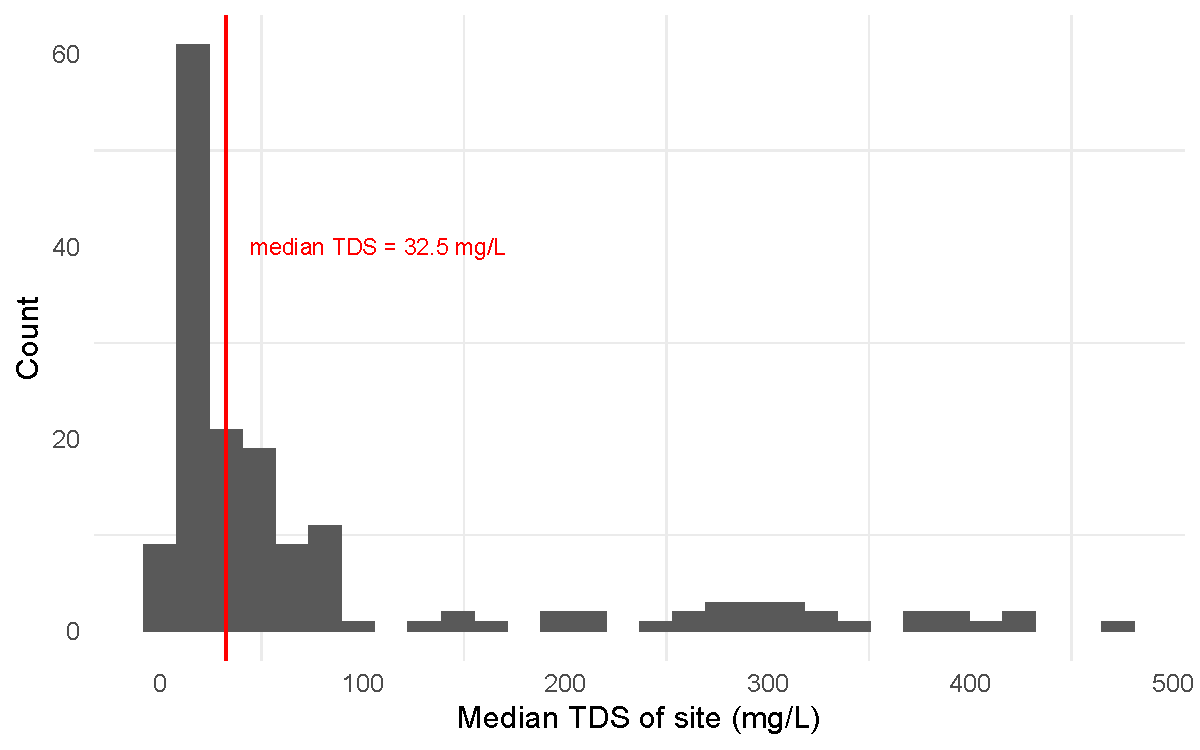
\includegraphics[width=\textwidth]{ch3_appendix_figs/natural_waters.pdf}
	\caption{Median TDS of natural waters measured at NWIS stations in Kern, Kings, Tulare, and Fresno counties*.}
	\label{ap_b_nat_waters}
\end{figure}

\egroup

*the following 162 NWIS station codes were analyzed: USGS-11186000, USGS-11187000, USGS-11191000, USGS-11194000, USGS-11203200, USGS-11203500, USGS-11204900, USGS-11206500, USGS-11206700, USGS-11206800, USGS-11206820, USGS-11208000, USGS-11208605, USGS-11208607, USGS-11208610, USGS-11208615, USGS-11208620, USGS-11208625, USGS-11208630, USGS-11208650, USGS-11208680, USGS-11208715, USGS-11208730, USGS-11209500, USGS-11210500, USGS-11210950, USGS-11212423, USGS-11213500, USGS-11218500, USGS-11220000, USGS-11221500, USGS-11221900, USGS-11222700, USGS-11230540, USGS-11247000, USGS-11250000, USGS-11251000, USGS-11253500, USGS-11254000, USGS-11256000, USGS-345002118424201, USGS-351355119194801, USGS-351745119203401, USGS-352641119404801, USGS-353328119395901, USGS-353933118274800, USGS-353953118234500, USGS-354144118263400, USGS-354251119373101, USGS-354307119351401, USGS-355428119234901, USGS-355802116555201, USGS-360039119583101, USGS-361419119511801, USGS-362100118454001, USGS-362102118241501, USGS-362102118402801, USGS-362243119471001, USGS-362317118245201, USGS-362511118245201, USGS-362540118452901, USGS-362542118432701, USGS-362629118245301, USGS-362647118360801, USGS-362718118244101, USGS-362730118281401, USGS-362730118343001, USGS-362730118400001, USGS-362808118242101, USGS-362808118242102, USGS-362852118240901, USGS-362937118200801, USGS-362947118193801, USGS-363010118302801, USGS-363107118453501, USGS-363112118454601, USGS-363113118480101, USGS-363138118445801, USGS-363310118240101, USGS-363331118450701, USGS-363438118243901, USGS-363455118251301, USGS-363616118245801, USGS-363623118441401, USGS-363629118424201, USGS-363634118444901, USGS-363820118253101, USGS-363911118315501, USGS-363922119402001, USGS-364000118404500, USGS-364019120321101, USGS-364101118412400, USGS-364153118344701, USGS-364155119445000, USGS-364155119445002, USGS-364203118345000, USGS-364218118343401, USGS-364234118404401, USGS-364235118345200, USGS-364236118411301, USGS-364247118352200, USGS-364345118345901, USGS-364400120202600, USGS-364406118382200, USGS-364427118373900, USGS-364454118370100, USGS-364510118262301, USGS-364511118260901, USGS-364519120222001, USGS-364646118320301, USGS-364647118321701, USGS-364658118371801, USGS-364659118372100, USGS-364712120230400, USGS-364718120221800, USGS-364723118403401, USGS-364732118360601, USGS-364746119445400, USGS-364754118344801, USGS-364809118413901, USGS-364818119443800, USGS-364818119464700, USGS-365016120261300, USGS-365027120313401, USGS-365035118321501, USGS-365035119555300, USGS-365105120293001, USGS-365130119504200, USGS-365130120265200, USGS-365202118303701, USGS-365226118255801, USGS-365235119465800, USGS-365235119470700, USGS-365238118260101, USGS-365338118320901, USGS-365453118313301, USGS-365543118444001, USGS-365650118403001, USGS-365743118382501, USGS-365808118375901, USGS-365845118373601, USGS-365912120300000, USGS-365922118264801, USGS-365940120300000, USGS-365952118351001, USGS-370000119393000, USGS-370025119414500, USGS-370059118394101, USGS-370102118391901, USGS-370111118344601, USGS-370140119393000, USGS-370312118342201, USGS-370515120321600, USGS-370539118350701, USGS-370555118354601, USGS-370847118462601, USGS-371017118424601, USGS-371025118432101, USGS-371033118423501, USGS-371123118473601, USGS-371127118454201, USGS-371212118480001


\clearpage


% 01_mm_plots_tables.R in F:/ ... POst_QE_Research/DISSERTATION/01_mm
% search for gw_and_sw_c_summary table


\bgroup

\renewcommand{\arraystretch}{1.5}

\begin{table}[H]
	
	\caption{TDS of natural waters (derived from NWIS samples, see Figure \ref{ap_b_nat_waters}) and agricultural diversions (derived from Central Valley Project and State Water Project water and salt budgets). $C$ is the concentration of TDS. From C2VSim, total applied water is 45.1\% agricultural diversions and 54.9\% groundwater pumping. Natural waters are the TDS of $R$, $B$, $C$, $I$, and $M$ in Table 1. Agricultural diversions are $D$ in Table \ref{ap_b_lsb}.}
	\centering
	
	\begin{tabular}{lr}
		
		\textbf{Source} & $\bm{C \: \: (mg/L)}$ \\ 
		\hline
		Natural waters & 32.50 \\ 
		Agricultural diversions & 264.53 \\ 
		\hline
	\end{tabular}
	
	\label{ap_b_gw_and_sw_c_summary}
\end{table}

\egroup



%--------------------------------------------------------%
\subsection{Spatial distribution of pre-1960 groundwater quality in the TLB}

% in F:\Box Sync\Research\Post QE Research\DISSERTATION\01_mm\code\02_reanalyze_gw_tds.R
% search predev_tds_map.pdf

\begin{figure}[H]
	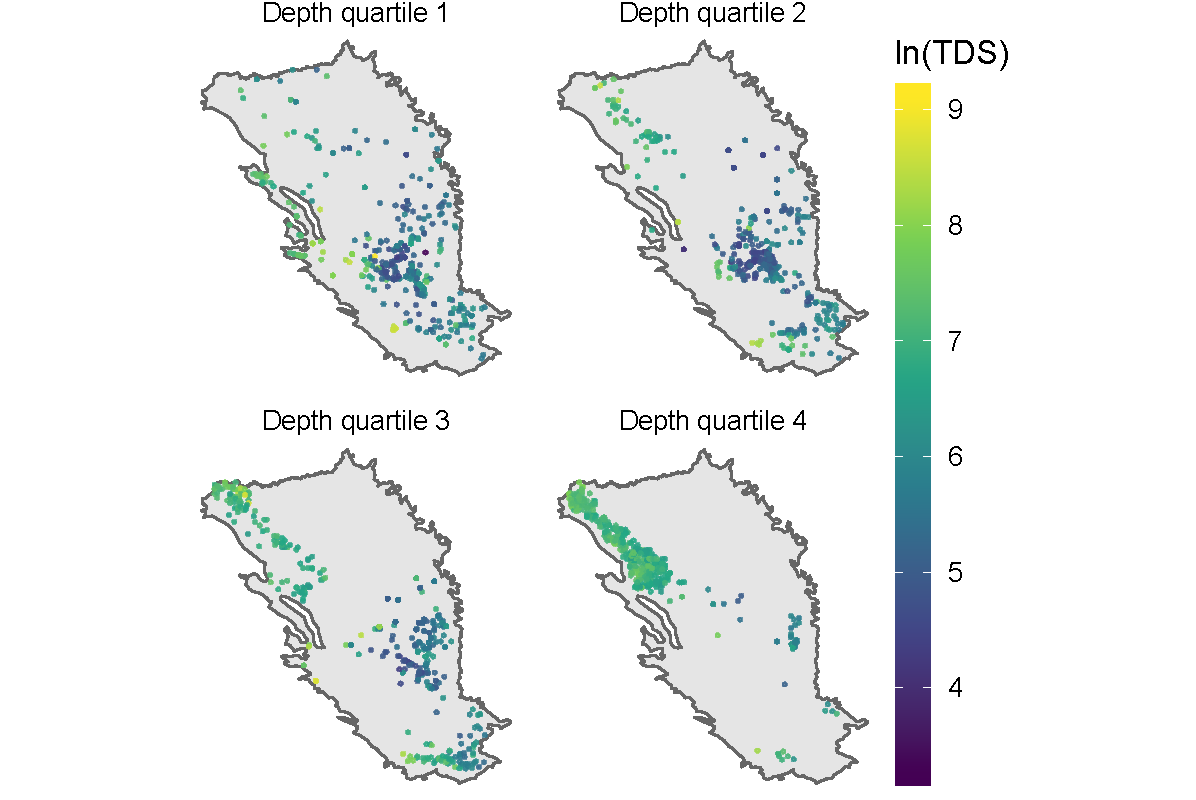
\includegraphics[width=\textwidth]{ch3_appendix_figs/predev_tds_map.pdf}
	\caption{Spatial distribution of pre-1960 groundwater quality (Figure \ref{fig:predev_tds_bc}) at 4 depth quartiles from land surface to 762 m in depth (near the base of fresh water). The mixing model (depth = 212 $m$) is contained within depth quartiles 1 and 2. Quartile 1 = 0.00 to -160.93 $m$, Quartile 2 = -160.94 to -256.03  $m$, Quartile 3 = -256.04 $m$ to -454.15, Quartile 4 = -454.16 to -762.00 $m$.}
	\label{ap_b_predev_tds_map}
\end{figure}


%--------------------------------------------------------%
\subsection{Vertical groundwater velocity in the TLB}


% velocity coefficients - perhaps in:
% 01_mm_plots_tables.R in F:/ ... POst_QE_Research/DISSERTATION/01_mm


\bgroup

\renewcommand{\arraystretch}{1.5}

\setlength{\tabcolsep}{20pt}

\begin{table}[H]
	
	\caption{Linear model coefficients for Equation (\ref{eq: vel}). The Darcy velocity ($m/yr$) at the top of cell $j$ = 1 is $\beta_0$, and decreases by $\beta_1$ with every vertical meter of depth. To account for groundwater velocity change in the alternate groundwater budget, groundwater velocity is scaled proportional to the decrease in vertical flow, $P_{alt}/(P - C)$, a 15 \% reduction. This is equivalent to the ratio of net downward flow in the alternate budget to the historical budget (Table 1).}
	
	\centering
	
	\begin{tabular}{ccc}
		
		$\bm{\beta_0}$ & $\bm{\beta_1}$ & $\bm{P_{alt}/P}$ \\ 
		\hline
		0.34 & -5.39E-4 & 0.85 \\ 
		\hline
	\end{tabular}
	
	\label{ap_b_velocity_coefficients}
\end{table}
\egroup




%--------------------------------------------------------%
\subsection{Porosity of sediments in the TLB}

% 07_johnson_porosity.R in F:/ ... POst_QE_Research/DISSERTATION/01_mm/code

\bgroup

\renewcommand{\arraystretch}{1.0}

\setlength{\tabcolsep}{1.0em}

\begin{table}[H]
	\caption{Sample mean porosities from Johnson (1968) Table 10.}
	
	\centering
	\fontsize{10}{10}\selectfont{
	\begin{tabular}{r}
		$\eta$\\
		\hline
		0.436\\
		0.327\\
		0.422\\
		0.406\\
		0.401\\
		0.446\\
		0.401\\
		0.423\\
		0.390\\
		0.423\\
		0.442\\
		0.407\\
		0.406\\
		0.391\\
		0.393\\
		0.375\\
		0.405\\
		0.397\\
		0.396\\
		0.369\\
		0.427\\
		0.438\\
		0.389\\
		0.440\\
		0.365\\
		0.395\\
		0.331\\
		0.356\\
	\end{tabular}
    }
	
	\label{ap_b_porosity_boot}
\end{table}

\egroup

\clearpage

% 07_johnson_porosity.R in F:/ ... POst_QE_Research/DISSERTATION/01_mm/code

\bgroup

\begin{figure}[H]
	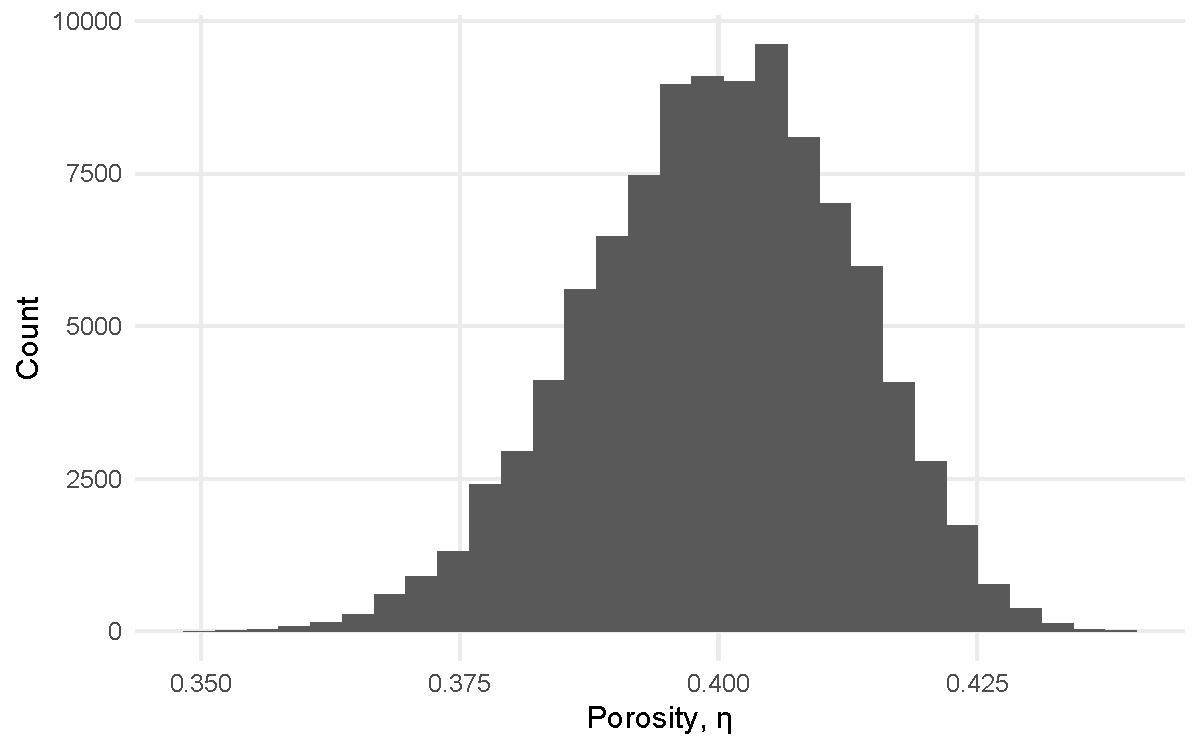
\includegraphics[width=\textwidth]{ch3_appendix_figs/porosity_boot.pdf}
	\caption{Sampling distribution of the porosity sample means from Johnson (1968), Table \ref{ap_b_porosity_boot}. The bootstrapped distribution of 100,000 samples of size n = 5 taken with replacement are approximately normal in distribution. Via the Central Limit Theorem, this indicates that the sampling distribution mean is approximately equal to the population mean. Thus, the sampling distribution mean (0.40) is used as the upscaled porosity in the mixing model. A single value is used because the interquartile range, bounded by 0.39 and 0.41, does not vary appreciably.}
	\label{ap_b_porosity_boot_hist}
\end{figure}

\egroup



%--------------------------------------------------------%
\subsection{Mixing cell model geologic and hydrologic parameters and mass balance error}


% 01_mm_plots_tables.R in F:/ ... POst_QE_Research/DISSERTATION/01_mm
%> c(Williamson, Kang) * 0.3048  # RWI
%[1] 0.243840 0.466055
%> (c(Williamson, Kang) * 0.3048)/2.71232 # divide by 1km unit depth of surface area (SA in km^3)
%[1] 0.0899009 0.1718289


%\bgroup

\renewcommand{\arraystretch}{1.5}

\setlength{\tabcolsep}{1.5em}

\begin{table}[H]
	
	\caption{Mixing cell model geologic and hydrologic parameters: $\eta$ is the porosity, $f$ is the aquifer fraction, $\rho$ is the rock-water interaction coefficient, and $E_a$ is the application efficiency. Ranges are provided for parameters used in the Monte Carlo simulation.}
	
	\centering
	
	\begin{tabular}{cccc}
		
		$\bm{\eta \:\: [-]}$ & $\bm{f \:\: [-]}$ & $\bm{\rho \:\: [mg/km^3]}$ & $\bm{E_a \:\: [-]}$\\ 
		\hline
		0.40 & 0.99 & 0.09 - 0.17 & 0.78 - 0.88\\ 
		\hline
	\end{tabular}
	
	\label{ap_b_geometry}
\end{table}

%\egroup



%--------------------------------------------------------%
%5\subsection{Mixing cell model mass balance error}



%\bgroup

\renewcommand{\arraystretch}{0.8}
\setlength{\tabcolsep}{3.5 em}


%\renewcommand{\arraystretch}{1.0}

% 01_mm_plots_tables.R in F:/ ... POst_QE_Research/DISSERTATION/01_mm
% average annual GW budget table - 1961-10-31 to 2001-09-30
% but a lot is added in the caption and table footnote, so beware changing this!!

\begin{threeparttable}
	
	\begin{table}[H]
		\centering
		\caption{Cell by cell budget and mass balance error, per equations (9) and (10).}
		
		
		\fontsize{8}{8}\selectfont{
		\begin{tabular}{rlrrrr}
			
			& \textbf{Source} & $\bm{Q \: \: (km^3/yr)}$ &  \\ 
			
			\hline
			\parbox[t]{2mm}{\multirow{7}{*}{\rotatebox[origin=c]{90}{\textbf{j = 1}}}}
			& $N$ & 1.883e+00 \\ 
			& $R$ & 2.451e+00 \\ 
			& $B$ & 2.355e-01 \\ 
			& $M$ & 6.784e-01 \\ 
			& $P_{alt, 1}$ & -3.040e-01 \\ 
			& $q_{1,2}$ & -4.944e+00 \\ 
			& $dS$ & 8.327e-17 \\ 
			\hline  
			\parbox[t]{2mm}{\multirow{5}{*}{\rotatebox[origin=c]{90}{\textbf{j = 2}}}}
			& $q_{1,2}$ & 4.944e+00 \\ 
			& $I_2$ & 6.194e-04 \\ 
			& $P_{alt, 2}$ & -2.864e-01 \\ 
			& $q_{2,3}$ & -4.658e+00 \\ 
			& $dS$ & -2.871e-16 \\ 
			\hline
			\parbox[t]{2mm}{\multirow{5}{*}{\rotatebox[origin=c]{90}{\textbf{j = 3}}}}
			& $q_{2,3}$ & 4.658e+00 \\ 
			& $I_3$ & 5.836e-04 \\ 
			& $P_{alt, 3}$ & -2.698e-01 \\ 
			& $q_{3,4}$ & -4.389e+00 \\ 
			& $dS$ & -1.717e-16 \\ 
			\hline
			\parbox[t]{2mm}{\multirow{5}{*}{\rotatebox[origin=c]{90}{\textbf{j = 4}}}}
			& $q_{3,4}$ & 4.389e+00 \\ 
			& $I_4$ & 5.499e-04 \\ 
			& $P_{alt, 4}$ & -2.542e-01 \\ 
			& $q_{4,5}$ & -4.135e+00 \\ 
			& $dS$ & 8.587e-17 \\ 
			\hline
			\parbox[t]{2mm}{\multirow{5}{*}{\rotatebox[origin=c]{90}{\textbf{j = 5}}}}
			& $q_{4,5}$ & 4.135e+00 \\ 
			& $I_5$ & 5.181e-04 \\ 
			& $P_{alt, 5}$ & -2.395e-01 \\ 
			& $q_{5,6}$ & -3.896e+00 \\ 
			& $dS$ & 2.676e-16 \\ 
			\hline
			\parbox[t]{2mm}{\multirow{5}{*}{\rotatebox[origin=c]{90}{\textbf{j = 6}}}}
			& $q_{5,6}$ & 3.896e+00 \\ 
			& $I_6$ & 4.882e-04 \\ 
			& $P_{alt, 6}$ & -2.257e-01 \\ 
			& $q_{6,7}$ & -3.671e+00 \\ 
			& $dS$ & -4.636e-16 \\ 
			\hline
			\parbox[t]{2mm}{\multirow{5}{*}{\rotatebox[origin=c]{90}{\textbf{j = 7}}}}
			& $q_{6,7}$ & 3.671e+00 \\ 
			& $I_7$ & 4.599e-04 \\ 
			& $P_{alt, 7}$ & -2.126e-01 \\ 
			& $q_{7,8}$ & -3.459e+00 \\ 
			& $dS$ & 1.494e-16 \\ 
			\hline
			\parbox[t]{2mm}{\multirow{5}{*}{\rotatebox[origin=c]{90}{\textbf{j = 8}}}}
			& $q_{7,8}$ & 3.459e+00 \\ 
			& $I_8$ & 7.498e-03 \\ 
			& $P_{alt, 8}$ & -3.466e+00 \\ 
			& $q_{8,9}$ & -6.250e-16 \\ 
			& $dS$ & -3.691e-16 \\ 
			\hline
			
		\end{tabular}
	}
		Cell by cell groundwater flows (Figure 3) are in steady state ($dS \approx MB_{error, j} \approx 0$). $N$ enters the top of the groundwater mixing cell model along with recharge from streams, lakes, and watersheds ($R$), boundary inflow from mountain front recharge ($B$), and managed aquifer recharge ($M$). Subsidence flow $C_{alt}$ = 0, per equation (\ref{eq: p_alt}). Subsurface inflow from the north ($I$) and pumping ($P$) are distributed proportional to cell volume ($V_j$). 
		
		\label{ap_b_cbc}
	\end{table}

\end{threeparttable}

%\egroup




% body of table is in MCMM_no_RWI_2.Rmd 
% print(xtable(t3), tabluar.environment = "longtable", include.rownames = FALSE)
% longtable example: http://users.sdsc.edu/~ssmallen/latex/longtable.html

%\bgroup

\renewcommand{\arraystretch}{0.7}

\setlength{\tabcolsep}{1.0em}

\begin{table}[H]
	\caption{Mixing model TDS-depth profile over time. Median and IQR refer to the median and interquartile range of TDS ($mg/L$) at the depth ($d$) of the cell bottom.}
	\centering
	
	\fontsize{9}{9}\selectfont{
		\begin{tabular}{@{\extracolsep{2 pt}}llllll@{}}
			
			&  & \multicolumn{2}{c}{\textbf{No RWI}} &  \multicolumn{2}{c}{\textbf{RWI present}}    \\ 
			\cline{3-4} \cline{5-6} \\ 
			$\bm{t \: (yrs)}$ & $\bm{d \: (m)}$ & \textbf{Median} & \textbf{IQR} &  \textbf{Median} & \textbf{IQR} \\ 
			\hline 
			
			\hline
			0 & 36 & 506 & 506-506 & 506 & 506-506 \\ 
			50 & 36 & 975 & 871-1124 & 1111 & 1007-1265 \\ 
			100 & 36 & 1101 & 961-1310 & 1369 & 1208-1603 \\ 
			150 & 36 & 1204 & 1029-1473 & 1600 & 1384-1922 \\ 
			200 & 36 & 1314 & 1100-1654 & 1836 & 1558-2264 \\ 
			250 & 36 & 1434 & 1176-1861 & 2081 & 1733-2638 \\ 
			300 & 36 & 1574 & 1264-2103 & 2345 & 1915-3057 \\ 
			\hline
			0 & 70 & 543 & 543-543 & 543 & 543-543 \\ 
			50 & 70 & 543 & 543-543 & 672 & 650-693 \\ 
			100 & 70 & 960 & 865-1094 & 1218 & 1128-1361 \\ 
			150 & 70 & 1113 & 977-1315 & 1493 & 1346-1729 \\ 
			200 & 70 & 1218 & 1047-1480 & 1717 & 1518-2045 \\ 
			250 & 70 & 1326 & 1116-1659 & 1945 & 1688-2383 \\ 
			300 & 70 & 1449 & 1195-1867 & 2188 & 1864-2743 \\ 
			\hline
			0 & 102 & 571 & 571-571 & 571 & 571-571 \\ 
			50 & 102 & 571 & 571-571 & 692 & 672-712 \\ 
			100 & 102 & 571 & 571-571 & 813 & 773-853 \\ 
			150 & 102 & 948 & 863-1070 & 1320 & 1231-1451 \\ 
			200 & 102 & 1120 & 988-1314 & 1606 & 1463-1830 \\ 
			250 & 102 & 1230 & 1063-1486 & 1829 & 1637-2144 \\ 
			300 & 102 & 1342 & 1136-1667 & 2056 & 1807-2485 \\ 
			\hline
			0 & 132 & 609 & 609-609 & 609 & 609-609 \\ 
			50 & 132 & 609 & 609-609 & 723 & 704-742 \\ 
			100 & 132 & 609 & 609-609 & 837 & 798-874 \\ 
			150 & 132 & 609 & 609-609 & 950 & 893-1007 \\ 
			200 & 132 & 938 & 861-1048 & 1409 & 1317-1532 \\ 
			250 & 132 & 1124 & 997-1310 & 1705 & 1565-1923 \\ 
			300 & 132 & 1245 & 1082-1494 & 1934 & 1742-2243 \\ 
			\hline
			0 & 160 & 637 & 637-637 & 637 & 637-637 \\ 
			50 & 160 & 637 & 637-637 & 744 & 726-762 \\ 
			100 & 160 & 637 & 637-637 & 851 & 816-887 \\ 
			150 & 160 & 637 & 637-637 & 959 & 905-1012 \\ 
			200 & 160 & 637 & 637-637 & 1066 & 994-1137 \\ 
			250 & 160 & 931 & 861-1030 & 1493 & 1388-1599 \\ 
			300 & 160 & 1131 & 1010-1308 & 1793 & 1650-2006 \\ 
			\hline
			0 & 187 & 656 & 656-656 & 656 & 656-656 \\ 
			50 & 187 & 656 & 656-656 & 757 & 740-773 \\ 
			100 & 187 & 656 & 656-656 & 858 & 824-891 \\ 
			150 & 187 & 656 & 656-656 & 959 & 908-1009 \\ 
			200 & 187 & 656 & 656-656 & 1060 & 992-1127 \\ 
			250 & 187 & 656 & 656-656 & 1161 & 1076-1245 \\ 
			300 & 187 & 930 & 867-1020 & 1562 & 1450-1670 \\ 
			\hline
			0 & 212 & 684 & 684-684 & 684 & 684-684 \\ 
			50 & 212 & 684 & 684-684 & 779 & 763-795 \\ 
			100 & 212 & 684 & 684-684 & 874 & 842-906 \\ 
			150 & 212 & 684 & 684-684 & 969 & 922-1017 \\ 
			200 & 212 & 684 & 684-684 & 1065 & 1001-1128 \\ 
			250 & 212 & 684 & 684-684 & 1160 & 1080-1239 \\ 
			300 & 212 & 684 & 684-684 & 1255 & 1159-1350 \\
			\hline
			
		\end{tabular}
	}
	\label{ap_b_p_sim}
\end{table}



% run for M with TDS = 0 mg/L  
% in MCMM.R change:
% annual_fluxes$TDS = c(0,gwc,gwc,gwc,gwc,gwc,0,gwc,0,gwc)
% to:
% annual_fluxes$TDS = c(0,gwc,gwc,gwc,gwc,gwc,0,gwc,0,0)
% Note the final value in the vector is the TDS of M, and changes from the gw concentration (104.6 mg/L) to 0 mg/L.

%\bgroup

\renewcommand{\arraystretch}{0.7}

\setlength{\tabcolsep}{1.0em}

\begin{table}[H]
	\caption{Mixing model TDS-depth profile over time when the TDS of $M$ = 0 $mg/L$. Median and IQR refer to the median and interquartile range of TDS ($mg/L$) at the depth ($d$) of the cell bottom.}
	\centering
	\fontsize{9}{9}\selectfont{

		\begin{tabular}{@{\extracolsep{2 pt}}llllll@{}}
			
			&  & \multicolumn{2}{c}{\textbf{No RWI}} &  \multicolumn{2}{c}{\textbf{RWI present}}    \\ 
			\cline{3-4} \cline{5-6} \\ 
			$\bm{t \: (yrs)}$ & $\bm{d \: (m)}$ & \textbf{Median} & \textbf{IQR} &  \textbf{Median} & \textbf{IQR} \\ 
			\hline 
			
			\hline
			0 & 36 & 506 & 506-506 & 506 & 506-506 \\ 
			50 & 36 & 963 & 859-1112 & 1099 & 995-1252 \\ 
			100 & 36 & 1086 & 945-1294 & 1354 & 1193-1587 \\ 
			150 & 36 & 1186 & 1012-1454 & 1582 & 1367-1903 \\ 
			200 & 36 & 1292 & 1080-1631 & 1814 & 1538-2241 \\ 
			250 & 36 & 1410 & 1153-1833 & 2057 & 1710-2611 \\ 
			300 & 36 & 1546 & 1238-2071 & 2317 & 1889-3026 \\ 
			\hline
			0 & 70 & 543 & 543-543 & 543 & 543-543 \\ 
			50 & 70 & 543 & 543-543 & 672 & 650-693 \\ 
			100 & 70 & 949 & 854-1083 & 1207 & 1117-1350 \\ 
			150 & 70 & 1098 & 962-1299 & 1478 & 1332-1713 \\ 
			200 & 70 & 1200 & 1030-1462 & 1699 & 1501-2026 \\ 
			250 & 70 & 1305 & 1096-1636 & 1923 & 1668-2361 \\ 
			300 & 70 & 1425 & 1173-1840 & 2163 & 1842-2717 \\ 
			\hline
			0 & 102 & 571 & 571-571 & 571 & 571-571 \\ 
			50 & 102 & 571 & 571-571 & 692 & 672-712 \\ 
			100 & 102 & 571 & 571-571 & 813 & 773-853 \\ 
			150 & 102 & 938 & 853-1060 & 1310 & 1221-1441 \\ 
			200 & 102 & 1105 & 974-1299 & 1591 & 1449-1815 \\ 
			250 & 102 & 1212 & 1045-1467 & 1811 & 1620-2126 \\ 
			300 & 102 & 1321 & 1117-1645 & 2035 & 1788-2462 \\ 
			\hline
			0 & 132 & 609 & 609-609 & 609 & 609-609 \\ 
			50 & 132 & 609 & 609-609 & 723 & 704-742 \\ 
			100 & 132 & 609 & 609-609 & 837 & 798-874 \\ 
			150 & 132 & 609 & 609-609 & 950 & 893-1007 \\ 
			200 & 132 & 929 & 852-1039 & 1400 & 1308-1523 \\ 
			250 & 132 & 1110 & 984-1295 & 1690 & 1551-1909 \\ 
			300 & 132 & 1228 & 1065-1476 & 1917 & 1725-2225 \\ 
			\hline
			0 & 160 & 637 & 637-637 & 637 & 637-637 \\ 
			50 & 160 & 637 & 637-637 & 744 & 726-762 \\ 
			100 & 160 & 637 & 637-637 & 851 & 816-887 \\ 
			150 & 160 & 637 & 637-637 & 959 & 905-1012 \\ 
			200 & 160 & 637 & 637-637 & 1066 & 994-1137 \\ 
			250 & 160 & 922 & 853-1022 & 1485 & 1380-1591 \\ 
			300 & 160 & 1117 & 996-1294 & 1779 & 1637-1992 \\ 
			\hline
			0 & 187 & 656 & 656-656 & 656 & 656-656 \\ 
			50 & 187 & 656 & 656-656 & 757 & 740-773 \\ 
			100 & 187 & 656 & 656-656 & 858 & 824-891 \\ 
			150 & 187 & 656 & 656-656 & 959 & 908-1009 \\ 
			200 & 187 & 656 & 656-656 & 1060 & 992-1127 \\ 
			250 & 187 & 656 & 656-656 & 1161 & 1076-1245 \\ 
			300 & 187 & 922 & 859-1013 & 1554 & 1442-1663 \\ 
			\hline
			0 & 212 & 684 & 684-684 & 684 & 684-684 \\ 
			50 & 212 & 684 & 684-684 & 779 & 763-795 \\ 
			100 & 212 & 684 & 684-684 & 874 & 842-906 \\ 
			150 & 212 & 684 & 684-684 & 969 & 922-1017 \\ 
			200 & 212 & 684 & 684-684 & 1065 & 1001-1128 \\ 
			250 & 212 & 684 & 684-684 & 1160 & 1080-1239 \\ 
			300 & 212 & 684 & 684-684 & 1255 & 1159-1350 \\ 
			\hline
			
		\end{tabular}
	}
	\label{ap_b_p_sim_m_with_tds_0}
\end{table}


%\clearpage



%--------------------------------------------------------%
% Acknowledgments
%--------------------------------------------------------%
\section{Acknowledgments}

We gratefully thank Drs. Helen Dahlke, Jonathan Herman, Randy Dahlgren, Laura Foglia, and Yong Zhang for their feedback and modeling advice. Dr. Can Dogrul and the California Department of Water Resources Groundwater Modeling division offered instrumental C2VSim modeling guidance. Support for this research was provided by the University of California Agricultural and Natural Resources grant CA-D-LAW-6036-H, the National Science Foundation (NSF) Climate Change, Water, and Society (CCWAS) Integrated Graduate Education and Research Traineeship (IGERT) program at the University of California, Davis (http://ccwas.ucdavis.edu, DGE-10693333), the U.S./China Clean Energy Research Center for Water-Energy Technologies (CERC-WET), and
the UC Office of the President’s Multi-Campus Research Programs and
Initiatives (MR-15-328473) through UC Water, the University of
California Water Security and Sustainability Research Initiative. All data is accessible via Dryad at \textit{https://datadryad.org/stash/dataset/doi:10.25338/B81P5K}, and procedures and models are accessible at \textit{https://github.com/richpauloo/Monte-Carlo-Mixing-Model} \citep{Pauloo2020}.  

\clearpage
\printbibliography[heading=bibliography]

% chapter 4
%\chapter{Real Title Here}
%--------------------------------------------------------%
%	TITLE
%--------------------------------------------------------%

\chapter[Mean flow direction modulates non-Fickian transport in a heterogeneous alluvial aquifer-aquitard system]{Mean flow direction modulates non-Fickian transport in a heterogeneous alluvial aquifer-aquitard system.\footnote[1]{This chapter will be submitted to \textit{Water Resources Research}: Pauloo, R. A., Fogg, G. E., Guo, Z. \& Henri, C. V. ``Mean flow direction modulates non-Fickian transport in a heterogeneous alluvial aquifer-aquitard system''.}}

%--------------------------------------------------------%
%	ABSRACT
%--------------------------------------------------------%
\section{Abstract}

\noindent Regional-scale groundwater quality degradation from nonpoint source pollution threatens the long-term %water quality 
sustainability of major alluvial aquifer-aquitard systems worldwide. Upscaled transport models can efficiently model regional nonpoint source transport, but fail to accurately characterize non-Fickian (anomalous) transport caused by transience in the mean flow direction. %Owing to the large spatial and temporal scale of nonpoint source pollution, the lack of field data, and uncertainty in geologic heterogeneity, upscaled contaminant transport models are needed. These upscaled models must accurately characterize non-Fickian (anomalous) transport caused by transience in the mean flow direction. 
In this study we demonstrate that hydrogeologic factors explain this failure. Specifically, vertical anisotropy in K and seasonal pumping and recharge in typical alluvial aquifer systems can %cause vertical hydraulic gradient values to exceed horizontal hydraulic gradient values by 10-100 times, 
fundamentally change hydraulic gradients and shift the mean flow direction between mostly horizontal and mostly vertical flow. In order to understand the relationship between large shifts in mean flow direction and transport phenomena, we simulate 3D flow and transport of a conservative solute in a heterogeneous alluvial aquifer under varying mean flow directions representative of typical seasonal hydraulic gradient fluctuations. We examine tailing, plume spreading, and the spatial distribution of final particle positions. Results indicate that alterations to hydraulic gradients which control the mean flow direction can lead to increasingly non-Fickian transport. %At low VHGR (e.g., ambient hydraulic gradient conditions that correspond to a more horizontal flow direction), 
When flow is mostly horizontal, diffusion and slow advection dominant low-K facies slow mass transfer rates out of low-K material, and preferential flow along connected high-K networks cause increased spatial spreading along the mean flow direction. In contrast, %high VHGR (e.g., 
predominantly vertical flow caused by spatially distributed pumping and recharge shifts mass transfer processes in low-K material from diffusion and slow advection dominant to advection dominant, which results in vertically oriented particle trajectories that compactly migrate through high and low K facies alike, and leads to increasingly Fickian transport. Thus, fluctuations in mean flow direction driven by vertical anisotropy of K and seasonal pumping and recharge in a typical alluvial aquifer-aquitard system create oscillating patterns of transport, ranging from persistently non-Fickian to more Fickian. Results %bear importantly on the management and modeling of widespread nonpoint source contamination in alluvial basins worldwide, and 
illustrate the hydrogeologic factors that explain why upscaled transport models fail to capture non-Fickian transience in mean flow direction.

%--------------------------------------------------------%
%	INTRO
%--------------------------------------------------------%
\section{Introduction}

Basin-scale groundwater quality in alluvial aquifer systems is threatened by nonpoint source contaminants including agricultural fertilizers \citep{Burow2008}, pesticides \citep{Burow2008, Burow1998}, nitrates \citep{Harter2012, henri2019stochastic}, and total dissolved solids \citep{Hansen2018, Lindsey2018} on large temporal (e.g., decades to centuries) and spatial scales (e.g., tens to hundreds of kilometers). Thus, regional groundwater quality management models \citep{Fogg2006} are needed that can robustly represent non-Fickian (i.e., anomalous) transport under a range of geologic heterogeneity and transient flow boundary conditions encountered on large temporal and spatial scales. However, modeling regional nonpoint transport remains a challenging task due to %differences between the temporal and spatial scales at which processes are typically measured and modeled \citep{cushman2002primer, bastani2020effects}, and due to 
ubiquitous non-Fickian spreading which is difficult to model at regional scales with existing approaches, especially when the boundary conditions shift from steady state to transient flow \citep{guo2020adaptive, labolle2001role}.

Transport modeling is challenged by non-Fickian transport across pore \citep{kang2014pore, morales2017stochastic}, field \citep{garabedian1991large, le2008non}, and regional scales \citep{sivakumar2005fractal, henri2019stochastic}, and in diverse heterogeneous geologic formations such as alluvial aquifers \citep{weissmann2002dispersion, labolle2001role, guo2019upscaling} and discrete fracture networks \citep{hyman2015influence, edery2016structural}. Non-Fickian transport may be measured by features including nonlinear scaling of the second spatial moment (i.e., the mean squared displacement), early breakthrough, and late-time arrival (i.e., tailing) of solutes \citep{valocchi1985validity, freyberg1986natural, zhang2007predicting, haggerty2000late}. The ubiquity of non-Fickian effects across disciplines and natural systems, and the inherent uncertainty in characterizing the scale and space-time dependencies of anomalous transport in heterogeneous media has led to multiple conceptualizations of how to mathematically model and upscale non-Fickian transport \citep{neuman2009perspective}.

Numerous studies show that anomalous transport in geologic media depends strongly on spatially heterogeneous hydraulic conductivity \citep{gelhar1993stochastic, dagan2005subsurface, de2005dealing}, which gives rise to the velocity field \citep{berkowitz2006modeling}. In many alluvial aquifer-aquitard complexes, variability in the hydraulic conductivity ($K$) of sediments can range over 4-7 orders of magnitude \citep{Fetter2001, fogg2016debates}. The fluvial deposition processes that form alluvial aquifer-aquitard systems over millennia result in correlated fields \citep{galloway2012terrigenous}, with interconnecting, high-K, coarse sand and gravel lenses \citep{fogg1986groundwater} that can percolate in all spatial dimensions \citep{fogg2000connected}, even at substantially low volume fractions, such as 13\% as noted in 3D percolation studies by \citet{harter2005finite}. These high-K preferential flowpaths facilitate anomalous early time arrival, and are embedded within low-K, fine-grained clays and silts, which typically comprise the majority of alluvial aquifer-aquitard volume fractions \citep{galloway2012terrigenous}, and contribute to mass hold back and anomalous late-time solute tailing \citep{labolle2001role, berkowitz2006modeling, haggerty2000late, benson2000application}. %Thus, stochastic hydrofacies models \citep<e.g.>{carle1996transition} which explicitly represent the geologic heterogeneity that gives rise to non-Fickian transport are a powerful tool to understand flow and transport properties of subsurface plumes, and have greatly informed the development of upscaled models \citep<e.g.>{guo2020adaptive}.

The interaction between spatial heterogeneity and hydraulics determines transport processes. However, anomalous transport studies commonly investigate simple hydraulic boundary conditions characterized by a unidirectional gradient \citep{benson2001fractional, edery2014origins, edery2016structural, harvey2000rate, pedretti2014apparent, willmann2008transport, leblanc1991large, julian2001numerical, Zhang1999nonideal, henri2015random}, which is typical of natural, ambient groundwater flow \citep[e.g. a horizontal hydraulic gradient on the order of $10^{-3}$][]{Fetter2001}. Many of these studies hold hydraulic boundary conditions constant in order to investigate how changing the spatial heterogeneity of the domain impacts solute transport. However, because of horizontal stratification of coarse- and fine-grained facies typical of many clastic sedimentary environments and hence significant vertical anisotropy of effective hydraulic conductivity (K), the vertical hydraulic gradients commonly exceed horizontal gradients by a factor of $10^1 - 10^2$ \citep[e.g.][]{fogg1986groundwater, belitz1993numerical}. In even moderately developed groundwater basins, and especially in agriculturally intensive ones, high rates of seasonal pumping and recharge from irrigation can further increase vertical hydraulic gradients \citep{styles1999subsurface, gailey2018using}. Yet, only a few modeling studies investigate non-Fickian transport under such large shifts in regional hydraulic gradient, and these studies tend to emphasize local scale breakthrough measured at extraction wells or control planes. \citet{matheron1980transport} demonstrated in a 2D model with limited spatial heterogeneity that flow parallel to the bedding direction leads to preasymptotic anomalous transport, even at very long timescales because the solute travels along an increasingly non-stationary medium. \citet{henri2019stochastic} demonstrated that well design characteristics (e.g., well depth, pumping rate, and screen length) have a significant impact on the uncertainty of late arrival times generated by heterogeneity. Similarly, \citet{libera2017influence} demonstrated that temporally variable pumping rates strongly affected contaminant breakthrough curves at the pumping well. \citet{guo2019upscaling} investigated anomalous transport arising from the transition from predominately horizontal to vertical flow, and found that internal hydraulic gradients between the high‐ and low‐K materials strongly affect mass transfer between hydrofacies. Furthermore, \citep{guo2020adaptive} showed that an upscaled multirate mass transfer model failed to capture tailing effects when the mean flow direction changed. Thus, prior work suggests that hydraulic boundary condition transience can strongly impact non-Fickian transport, we still lack an understanding of how shifting hydraulic gradients (as opposed to the unidirectional gradient that most studies explore) may modulate the degree of anomalous transport observed in a heterogeneous aquifer-aquitard complex. 

To the best of our knowledge, no studies have investigated the impact of mean flow direction on non-Fickian transport within a 3D, kilometer-scale, alluvial aquifer-aquitard system. Such a question bears importantly on modeling macroscopic nonpoint source transport in large alluvial groundwater systems, and may shed light on how to build better upscaled transport models that perform well across a range of transient hydraulic gradient conditions.

In this study, we simulate groundwater flow and random walk particle tracking in a detailed hydrofacies model of a typical alluvial aquifer-aquitard complex (with high vertical anisotropy in K) subject to an increasingly high \textbf{v}ertical to \textbf{h}orizontal hydraulic \textbf{g}radient \textbf{r}atio (VHGR), which is an indicator of the mean flow direction. In other words, if we increase the vertical hydraulic gradients in a system by a factor of 10, 100, or 1000 (e.g., due to natural geologic variation in vertical anisotropy of K, or during the transition from a fallow winter season to a summer growing season characterized by pumping and recharge), does this makes the transport more non-Fickian, and if so, by how much, and why? Changes in anomalous nonpoint source transport are compared between differing steady-state VHGR scenarios which collectively represent snapshots along a transition from predominantly horizontal (low VHGR) to vertical flow (high VHGR). We examine tailing, spatial variance of the nonpoint source plume, and the spatial distribution of final particle position to quantify and explain differences in non-Fickian spreading. Results are discussed in the context of the transition from advection to diffusion dominant systems, and related to the hydrogeology of the study site. We explore how our findings support a conceptualization of regional scale nonpoint source contaminant migration characterized by oscillating patterns of non-Fickian transport, and how this perspective might inform the development of upscaled regional groundwater quality management models \citep{Fogg2006}.




%--------------------------------------------------------%
%	METHODS
%--------------------------------------------------------%
\section{Methods}

First, a heterogeneous, hydrofacies-based geostatistical model of the Kings River alluvial fan in California's Central Valley was developed. Next, four VHGR scenarios of increasingly vertical groundwater flow were simulated, and used to solve the particle transport of a conservative solute. Lastly, the resulting 3D Lagrangian particle trajectories were analyzed in terms of their tailing, second spatial moment, and spatial distribution of final particle position. 

%
%---------------- Hydrofacies model  ------------------%
%
\subsection{Heterogeneous hydrofacies model and study site}
\label{ss_2_1}

The three‐dimensional, spatially-correlated hydraulic conductivity domain (Figure \ref{fig:model}) was simulated with Transition Probability Geostatistical Software (T-PROGS), which uses the transition probability approach described by \citet{carle1996transition, carle1997modeling, carle1999tprogs}. Details of the facies model are provided in \citet{weissmann1999three, weissmann1999multi, weissmann2002glacially, weissmann2004influence}, and a brief summary is provided here.

A subsection of the Central Valley aquifer (California, USA) in the Kings River fan, was chosen as a study site representative of a typical alluvial aquifer for its high vertical anisotropy ($K_h/K_v =$ 238), and its validated performance in simulating both flow (hydraulic head) and transport (groundwater age distribution) \citep{weissmann2002dispersion}. The hydrofacies model was conditioned by analyzing more than 40 000 surface and shallow subsurface ($<$ 2 $m$) features (e.g., borings, excavations, road cuts, and natural exposures) \citep{huntington1981soil}, approximately 150 $m$ of core and geophysical logs \citep{burow1997hydrogeologic}, approximately 1,000 $m$ of continuous core \citep{harter2005deep}, and numerous drillers' logs from water wells in the study area \citep{weissmann1999multi}. These analyses defined a conceptual geologic model and the T-PROGS model parameters. 

The Kings River alluvial fan is composed of four sequences created during Pleistocene glacial cycles and a fifth basal depositional unit prior to major glaciation events, each separated by laterally-extensive paleosols that formed during inter-glacial periods of pedogenesis \citep{weissmann2002glacially}, which, owing to their relatively low hydraulic conductivity, act as aquitards. Notably, one unit represents a incised valley fill of coarse-grained sediment, created by large glacial outwash in the east-west $y$ direction of the domain. Key parameters derived from these analyses that constrained the T-PROGS model include the hydrofacies proportions, mean lengths in $xyz$, and the embedded transition probabilities in $xyz$, which reflect the cross-correlation between facies and thus the probability that one facies contacts another in a given direction \citep{carle1996transition}. Next, Markov chain models corresponding to each unit were developed and combined to represent the highly heterogeneous stratigraphy: overlapping alluvial fans, interspersed with laterally-extensive paleosols, and a cross-cutting incised valley fill. \citet{weissmann2004influence} provides a detailed overview of the development and combination of these models into a single conductivity field. 


% F:\Box Sync\Research\Post QE Research\DISSERTATION\02_ade\code\00_interpolate_paths_extract_trajectories.R
% creates: C:/Users/rpauloo/Documents/GitHub/kings-river-fan-tprogs/code/rw3d//2019_11_20_100s_10kp/dat/part_traj_paraview_00_03.csv
% which is read into Paraview, and edited in Illustrator in C:\Users\rpauloo\Documents\GitHub\kings-river-fan-tprogs\paraview
% Paraview: krf_plus_part_traj_FINAL_00_03.pvsm
% AI: krf_part_traj_00_03.ai
% PNG: krf_part_traj_00_03-01.png
% 01_mm\ai\study_site_water_budget.ai
% numbers come from archived (commented out Table 5)
\begin{figure}[ht]
\centering
  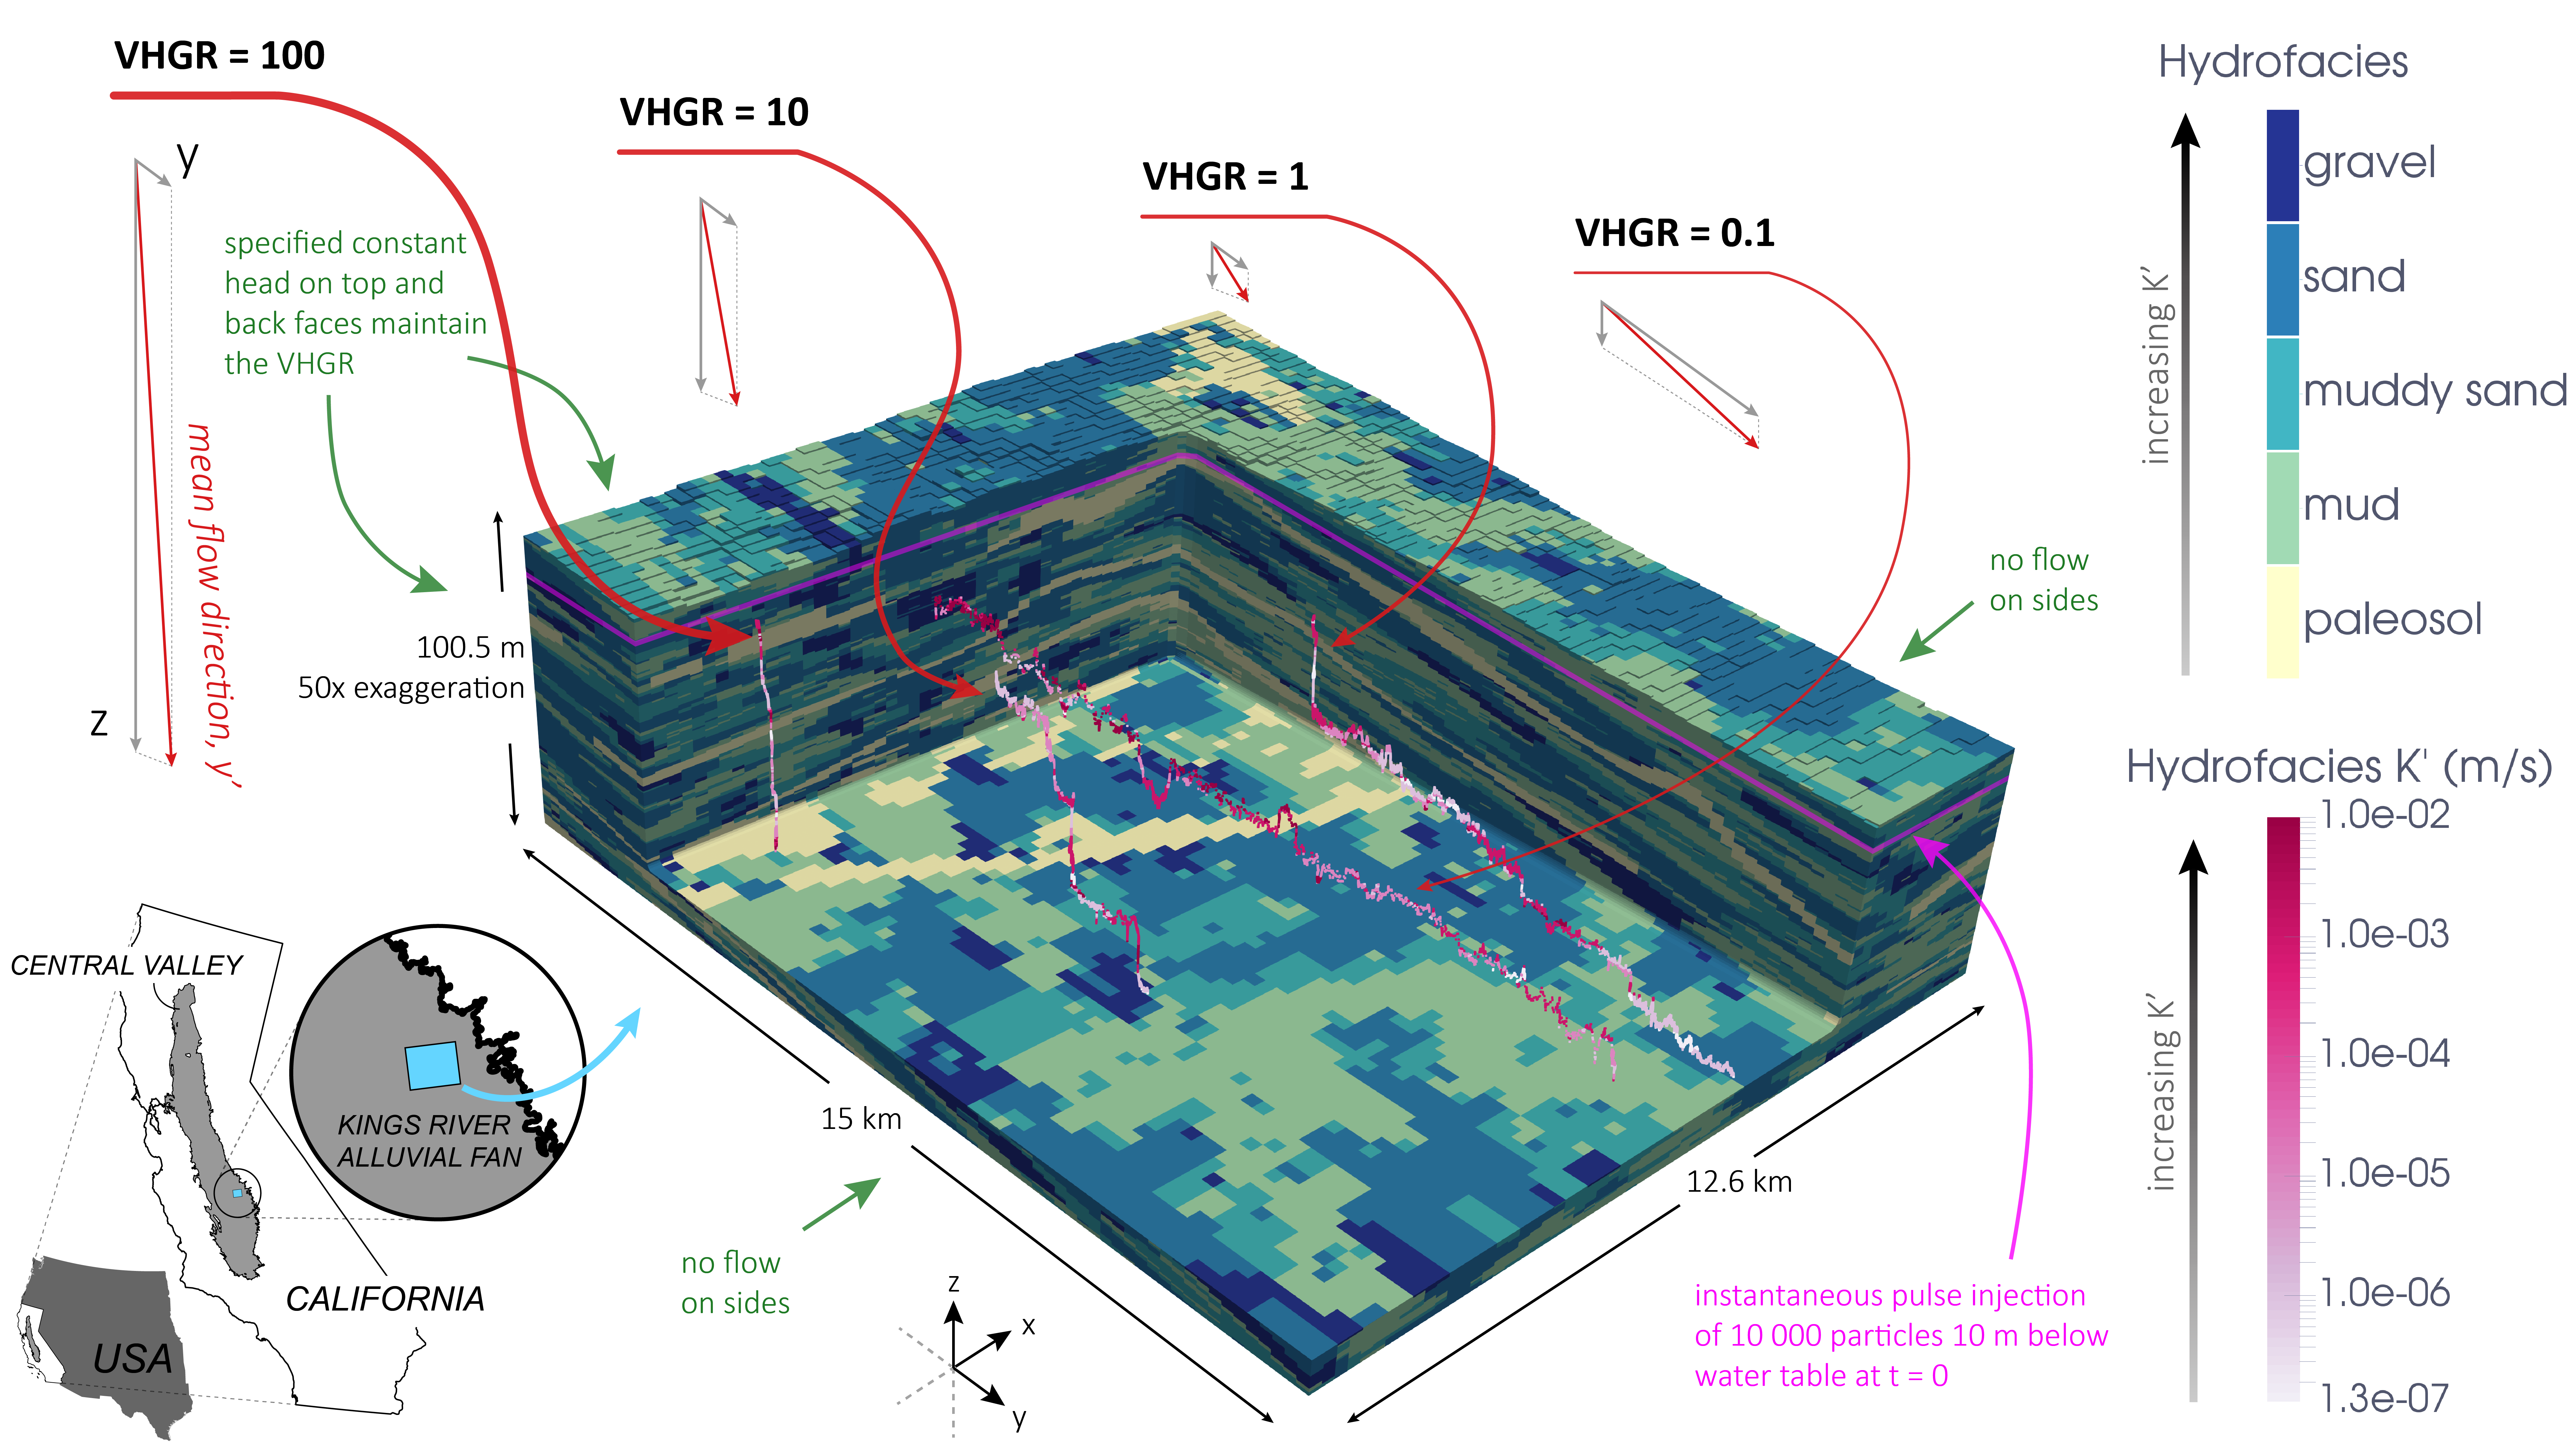
\includegraphics[width=\textwidth]{ch4_figs/krf_part_traj_00_03-01.png}
  \caption{The Kings River alluvial fan hydrofacies model in California's Central Valley (USA) with a section cut away to reveal the geologic heterogeneity and four representative particle trajectories from the four VHGR scenarios in this study (section \ref{ss_2_3}). The location of the instantaneous nonpoint source term (10 000 particles, 10 $m$ below the water table) is represented by a horizontal pink line. Particle trajectories are increasingly horizontal and non-Fickian with decreasing VHGR. Note that the vectors representing flow in $z$, $y$, (and their geometric sum in the mean flow direction, $y'$) are illustrative, and not drawn to scale.}
  \label{fig:model}
\end{figure}


The model dimensions in $xyz$ are 12.6 $km$ x 15 $km$ x 100.5 $m$, with discretization $\Delta x = \Delta y = $ 200 $m$, and $\Delta z =$ 0.5 $m$. Spatially variable $K$ estimated from pumping tests, slug tests, core measurements, and literature values for similar lithologies \citep{burow1999evaluation, weissmann1999three} were assigned to each of the model cells by their simulated hydrofacies, which include gravel, sand, sandy mud, muddy sand, and paleosols (Table \ref{tab:model_l_k_pe}).


% F:\Box Sync\Research\Post QE Research\DISSERTATION\02_ade\code\tables.R
% object is called `d`
\bgroup
\begin{table}[ht]
\centering
%\small\addtolength{\tabcolsep}{-5pt}
\resizebox{\textwidth}{!}{%
\begin{tabular}{lrrrlllll}
\hline
Hydrofacies & $l_x (m)$ & $l_y (m)$ & $l_z (m)$ & $K (m/s)$ & $P_e^{100}$ & $P_e^{10}$ & $P_e^{1}$ & $P_e^{0.1}$\\

\hline

gravel & 200 & 650 & 1.5 & 1.0E-02 & 2.05E+09 & 2.05E+08 & 2.05E+07 & 2.05E+06\\
sand & 625 & 1500 & 3.3 & 1.0E-03 & 5.13E+08 & 5.13E+07 & 5.13E+06 & 5.13E+05\\
muddy sand & 400 & 800 & 1.4 & 1.0E-05 & 2.90E+06 & 2.90E+05 & 2.90E+04 & 2.90E+03\\
mud & NA & NA & 1.0 & 1.0E-06 & 289.86 & 28.99& 2.9 & 0.29 \\
paleosol & 800 & 1500 & 1.9 & 1.3E-07 & 71.59 & 7.16 & 0.72 & 0.07\\

\hline
\end{tabular}
} % for \resizebox
\caption{Hyrdofacies properties including mean lengths $l$ in $xyz$ directions (strike, dip, and vertical in Figure \ref{fig:model}), hydraulic conductivity $K$ ($m/s$), and average Peclet number across the VHGR scenarios.}
\label{tab:model_l_k_pe}
\end{table}

\egroup

We only use one realization of the hydrofacies model (Figure \ref{fig:model}) because previous studies demonstrate that non-Fickian transport behavior does not appreciably differ between realizations due to good connectivity of aquifer facies \citep{guo2019upscaling, weissmann2002dispersion}.


%
%---------------- Groundwater flow simulation  ------------------%
%
\subsection{Groundwater flow and transport simulation}
\label{ss_2_2}

Steady state, groundwater flow in the geostatistical model grid (Section \ref{ss_2_1}) is simulated in MODFLOW \citep{harbaugh2000modflow, mcdonald1988modflow}. The 3D groundwater flow equation used to compute long-term, average confined flow is:   


\begin{equation}
    \frac{\partial{}}{\partial{x}}(K_{xx} \frac{\partial{h}}{\partial{x}}) +
    \frac{\partial{}}{\partial{y}}(K_{yy} \frac{\partial{h}}{\partial{y}}) +
    \frac{\partial{}}{\partial{z}}(K_{zz} \frac{\partial{h}}{\partial{z}}) +
    W = S_s \frac{\partial{h}}{\partial{t}}
\label{eq:gwflow}
\end{equation}

where $K_{xx}$, $K_{yy}$, and $K_{zz}$ [$LT^{-1}$] are the hydraulic conductivities along the $x$, $y$, and $z$ coordinate axes; $h$ $[L]$ is the potentiometric head; $W$ [$T^{-1}$] is the volumetric flux per unit volume of sources ($W >$ 0) or sinks ($W <$ 0); $S_s$ [$L^{-1}$] is the specific storage; and $t$ $[T]$ is time. 

The water table is represented on the top of the domain with a constant head boundary condition, which is the same across all scenarios. Vertical flow out of the bottom of the model and into deeper groundwater, due to a combination of pumping at depth and recharge from above, is represented by another constant head boundary condition on the bottom of the domain, and is altered depending on the VHGR scenario in question (discussed in section \ref{ss_2_3}). Two more constant head boundary conditions on the front and back faces of the model maintain a horizontal groundwater flow gradient of 0.001 along the $y$ direction (Figure \ref{fig:model}), and represent mountain front recharge along the eastern model boundary. Head values are spatially distributed across all active faces such that the mean flow direction is uniform across the entire domain (SI Appendix Figure \ref{ap_c_heads_vhgr}). No flow boundaries are specified along the right and left faces of the domain (along the $x$ direction). 


%Particle tracking transport simulation

Solute transport is simulated by the random‐walk particle tracking method \citep{labolle1998diffusion, labolle2000diffusion} applied in the code RW3D \citep{fernandez2005differences, henri2014toward, henri2015random, salamon2006modeling} that solves the advection-dispersion equation: 

\begin{equation}
    \theta \frac{\partial{c}}{\partial{t}} = \nabla \cdot (\theta D \nabla c) - \nabla \cdot (qc)
\label{eq:ade}
\end{equation}

%\begin{equation}
%    D = (\alpha_T |q| + D^*) \delta + (\alpha_L - \alpha_T)qq^t / |q|
%\label{eq:d}
%\end{equation}

where $c$ is the concentration of the dissolved solute [$ML^{-3}$], $\theta$ is the effective porosity [$-$], and $\textbf{D}$ is the dispersion tensor, defined as $\textbf{D} = (\alpha_T |\textbf{q}| + D^*) \textbf{I} + (\alpha_L - \alpha_T) \textbf{qq}^t / |\textbf{q}|$, where $D^*$ is the molecular diffusion coefficient [$L^2 T^{-1}$], $\alpha_L$ and $\alpha_T$ are the longitudinal and transverse dispersivities [$L$], $\textbf{I}$ is the Dirac delta function, and $|\textbf{q}|$ is the magnitude of the velocity vector [$LT^{-1}$].

The source term is a discrete, instantaneous pulse injection of 10 000 particles at 10 $m$ below the water table (Figure \ref{fig:model}). To simulate the spatial variability of contaminant mass arrival at the water table, flux-weighted injection is used to initialize particle motion. Simulations are run for a sufficient number of time steps such that all particles exit the domain (SI Appendix Table \ref{ap_c_rw3d_params}), and that the mean Lagrangian hydrofacies proportions (i.e., the proportion of particles in each hydrofacies) converge on the actual hydrofacies proportions over time (SI Appendix Figure \ref{ap_c_heads_vhgr}). The Lagrangian particle tracking methods used in this study can be very computationally intensive, especially for the case of a regional-scale nonpoint source term, where the size of the domain (and hence the number of particles used to sample it) is large. Adding multiple injections of particles was computationally unrealistic, and moreover, under steady state flow, a continuous source injection and instantaneous pulse injection yield similar results. %(this is not the case for a transient flow simulation, which we do not investigate). 

\citet{labolle2001role} demonstrated for a similar hydrofacies-based domain that solute transport results were insensitive to local-scale $\alpha$, which was insignificant compared to the dispersion caused by the hydrofacies-scale heterogeneity of the conductivity domain. Moreover, \citet{weissmann2002dispersion} investigated sensitivity analyses with $\alpha_L$ and $\alpha_T =$ 0.1 $m$ and $=$ 0.01 $m$ in the same Kings River Fan domain that we use in this study, and found that between geostatistical realizations, the simulation results did not differ appreciably in terms of the overall transport. Thus, we set longitudinal, transverse horizontal, and transverse vertical dispersivities to 0.01 times the cell discretization, $\alpha_L = \alpha_{TH} = $ 2.0 $m$, and $\alpha_{TV} = $ 0.005 $m$. These local-scale dispersivities were maintained across the VHGR scenarios in order to ensure comparability. We assume a conservative (non-reactive, non-sorbing) solute and set the molecular diffusion coefficient $D^*$ = 6.9E-10 $m^2/s$, based on \citet{weissmann2002dispersion}. 

% $D^* = D_d / \tau^2$ \citep{Fetter2001}, where $D_d$ is an average diffusion coefficient for common ions, 2.0E-9 $m^2/s$, \citep{domenico1998physical} and $\tau$ is an average tortuosity (arc to chord ratio) of 1.7, according to



%---------------- hydraulic gradient scenarios  ------------------%
\subsection{Hydraulic gradient scenarios}
\label{ss_2_3}

This aim of this study is to investigate the influence of mean flow direction on non-Fickian transport, thus we compare systems under different \textbf{v}ertical to \textbf{h}orizontal \textbf{g}radient \textbf{r}atio (\textbf{VHGR}):

\begin{equation}
    VHGR = i_v / i_h
\label{eq:vhgr}
\end{equation}

where $i_v$ is the vertical gradient $\partial{h}/\partial{z}$, and $i_h$ is the horizontal gradient $\partial{h}/\partial{y}$ (Figure \ref{fig:model}). Increasing VHGR corresponds to increasingly vertical flow. Four scenarios are simulated, in which VHGR is varied over four orders of magnitude by fixing $i_h$ = 0.001 (representing ambient horizontal groundwater flow from mountain front recharge), and adjusting $i_v$:

\begin{itemize}
    \item VHGR = 0.1 ($i_v =$ 0.0001): primarily horizontal flow with minimal recharge
    \item VHGR = 1 ($i_v =$ 0.001): equal horizontal and vertical gradients  
    \item VHGR = 10 ($i_v =$ 0.01): substantial component of vertical groundwater flow
    \item VHGR = 100 ($i_v =$ 0.1): dominantly vertical flow 
\end{itemize}

Because of the strong vertical anisotropy caused by the stratified interbedding of coarse and fine facies, the ratio between effective $K_h$ and $K_v$ in our study site is 238, which tends to produce natural values of VHGR $>$ 1 in such systems \citep[e.g.][]{fogg1986groundwater}. Groundwater development by pumping can further increase VHGR, and the augmentation of recharge due to irrigation can still further increase it. For example, values of $i_v$ in portions of the Central Valley can vary from order $10^{-3}$ in winter (non-pumping season) to $10^{-1}$ in summer (pumping season). Hence, taken independently, the four steady state VHGR flow fields represent stages along a transition from ambient, primarily horizontal groundwater flow to predominantly vertical flow induced by natrual anisotropy in K and pumping and recharge, and permit an investigation of long-term plume evolution across these different hydraulic gradient conditions. 


Across each VHGR, the Peclet number, $P_e$ (i.e., the ratio of the characteristic time scales of advection to diffusion) was calculated for each hydrofacies (Table \ref{tab:model_l_k_pe}).

\begin{equation}
    P_e = K i l \: / \: D^* \theta
\label{eq:pe}
\end{equation}

where $i$ is the vertical hydraulic gradient of the VHGR scenario and $D^* =$ 6.9E-10 $m^2/s$ \citep{weissmann2004influence, weissmann2002modeling}, and $\theta$ is the hydrofacies porosity. Due to the influence of vertical gradients, $P_e$ of gravel, sand, and muddy sand were calculated using mean horizontal length scales ($l_x, \: l_y$), whereas the $P_e$ of mud and paleosol were calculated using vertical length scales ($l_z$). For gravel, sand, and muddy sand, $\theta =$ 0.3, and for mud and paleosol, $\theta =$ 0.5. Mud was used as a background category, thus its lateral mean lengths ($l_x$ and $l_y$) were already determined in the process of Markov chain modeling of the transition probability \citep{weissmann1999three}.


Generally, system-wide $P_e > 1$ is considered advection dominant, $P_e < 1$ indicates diffusion dominance, and slow advection (which may resemble a more diffusion-like process) may occur at relatively small $P_e$ less than 1 \citep{guswa2000slow}. In heterogeneous aquifer-aquitard systems, which vary in terms of the hydraulic conductivity field, porosity, and hydraulic gradient, $P_e$ varies spatially. Importantly, the $P_e$ of low-K mud and paleosol hydrofacies in this study can transition between advection and diffusion dominance due to changes in flow rates in these hydrofacies caused by different VHGR, with consequences for macroscopic transport behavior. 






%
%---------------- Metrics of non-Fickian transport  ------------------%
%
\subsection{Metrics of non-Fickian transport}
\label{ss_2_5}

In order to compare the impact of various VHGR scenarios on anomalous transport, we measure tailing by fitting a tempered fractional advection-dispersion equation (TFADE) to breakthrough curves and comparing the tempering parameter. Tailing is the late-time arrival of solutes at a control plane, and indicates mass holdback in fines. We also compute the time and space evolution of the mean squared displacement (MSD), or second spatial moment, which measures the variance in plume displacement and represents how ``spread out'' all of the particles are from one another due to mass holdback and preferential flow. Lastly, we investigate the spatial distribution of final particle positions with respect to the site's geologic heterogeneity, which illustrates preferential flow.

Between VHGR scenarios, travel times are re-scaled by $t_c = l_c / \bar{v}$, where $t_c$ is the characteristic travel time to travel the average facies length, and $l_c$ and $\bar{v}$ are the characteristic length and mean velocity along the mean flow direction $y'$ (details provided in SI Appendix Section \ref{s_ap_c_part_rot} and Table \ref{ap_c_tc}). 


%
%---------------- Tailing  ------------------%
%
\subsubsection{Tailing}
\label{ss_tailing}

In order to quantify differences in tailing, a tempered fractional advection-dispersion equation (TFADE) model \citep{meerschaert2008tempered} was fit to breakthrough at a control plane along the bottom face of the model:

\begin{equation}
\label{eq:tfade}
    \frac{\partial C(y', t)}{\partial t}+\beta e^{-\lambda t} \frac{\partial^{\gamma}\left[e^{\lambda t} C(y', t)\right]}{\partial t^{\gamma}}-\beta \lambda^{\gamma} C(y', t)=-V_{L} \frac{\partial C(y', t)}{\partial y'}+D_{L} \frac{\partial^{2} C(y', t)}{\partial y'^{2}}
\end{equation}

where $t$ $[T]$ is time; $C$ $[ML^{-3}]$ is the concentration; $y'$ $[L]$ is the position along the longitudinal direction; $V_L$ $[LT^{-1}]$ is the longitudinal velocity; $D_L$ $[L^2T^{-1}]$ is the molecular dispersion coefficient; $\beta$ $[T^{\gamma^{-1}}]$ is the fractional capacity coefficient, which governs the mobile fraction; $\gamma$ $[-]$ is the time fractional order; $\lambda$ $[T^{-1}]$ is the tempering parameter. Importantly, $\lambda$ represents the probability that the waiting times in the immobile phase transfer from a power‐law to exponential distribution and thus, provides a quantitative measure of tailing: as $\lambda$ approaches infinity, the TFADE reverts to the classic advection-dispersion equation, and a decreasing $\lambda$ indicates longer tailing. 

It was assumed that the sample of initial particles that exit the bottom face of the domain represented macroscopic breakthrough along this plane if the domain was infinitely wide in the $x$ and $y$ dimensions, and if simulation time was unlimited. As VHGR decreases, horizontal flow causes more particles to exit the down-gradient face, yet a substantial fraction of 10 000 initial particles exit the bottom face in each simulation: 78.0, 74.7, 16.8, 7.7 \% of particles break through the bottom of the domain after 1000 characteristic times in VHGR = 100, 10, 1, and 0.1 respectively. 
% 03_residence_time_distribution.R    rt %>% filter(z <= 1) %>% count(sim) %>% pull(n)/10000*100


%
%---------------- Spatial variance - MSD  ------------------%
%
\subsubsection{Spatial variance}
\label{ss_msd}

Next, the time evolution of the plume spatial variance is calculated. The mean squared displacement along a given direction $x$ is:  

\begin{equation}
\label{eq:msd}
    \sigma_{x}^2 = \left\langle (x(t) -  \left\langle x(t) \right\rangle)^2 \right\rangle
\end{equation}

where $\left\langle \cdot \right\rangle$ denotes the average position in the $x$ direction over all particles, and every particle is first initialized to an identical reference location (i.e., centered spatial moment). We calculate the spatial variance in the longitudinal, transverse vertical, and transverse horizontal directions using (\ref{eq:msd}). Fickian diffusion occurs when the plume MSD varies as $t^{\phi}$, where $\phi = $ 1 \citep{berkowitz1991dispersion, neuman1990universal}. By contrast, non-Fickian transport occurs when $\phi$ does not equal unity. Super- and subdiffusion refer to $\phi > $ 1 and $\phi < $ 1 respectively. In order to ensure the MSD represented an accurate measure of macroscopic spatial variance of the plume (and not boundary effects created by early exiting particles), we restrict our analysis of the MSD results to before 32 characteristic time scales ($t/t_c \approx 10^{1.5}$). %when approximately 95.4, 87.8, 62.5, 59.5 \% of particles remain in VHGR = 100, 10, 1, and 0.1 respectively. Decreasing particle proportions as VHGR decreases are due to particles with short residence times that take horizontal flowpaths out of the top and down-gradient sides of the model, discussed more thoroughly in Sections \ref{ss_3_3} and \ref{ss_4_2}. 
% 02_ade/code/03_residence_time_distribution:   100-100*(bind_rows(ll) %>% filter(log_t_ta >= 1.5 & log_t_ta <= 1.6) %>% group_by(sim) %>% slice(1) %>% pull(cbtc) %>% rev() )


%
%---------------- Residence time and final particle position  ------------------%
%
\subsubsection{Final particle position}
\label{ss_rtd_pp}

Lastly, we compare %the range and tailing of the particle residence time distribution across VHGR scenarios. The residence time of a particle is the time at which it exits the domain, which can be thought of as breakthrough at a control plane along any of the faces of the domain. We relate differences in the particle residence time distribution to the 
spatial distribution of final particle positions (i.e., the location at which particles exit the domain), and the geologic heterogeneity of the domain. The spatial patterns of particle exit points strongly illustrate preferential flow along high-K hydrofacies and lend insight into transport dynamics across VHGR scenarios.







%--------------------------------------------------------%
%	RESULTS
%--------------------------------------------------------%
\section{Results}
\label{s_3}

%We simulated 3D flow and particle transport in a highly heterogeneous alluvial aquifer along a range of VHGR corresponding to increased pumping and recharge that would cause the transition between relatively horizontal ambient flow (VHGR = 0.1) to predominately vertical flow (VHGR = 100). In order to investigate non-Fickian transport between the VHGR scenarios, we measured mean squared displacement, compared the range and tailing in the particle residence time distribution, analyzed the spatial distribution of final particle positions with respect to residence time and domain geology, and fit a TFADE model to breakthrough along the bottom face of the model to quantify late time tailing. 


%
%----------- TFADE ---------------%
%

\subsection{Tailing in breakthrough}
\label{ss_3_1}

Tailing is quantified in the vertical dimension, because downward contaminant migration is of practical concern to water quality in groundwater wells, and exacerbates site cleanup efforts. We fit a TFADE model \citep{meerschaert2008tempered} to breakthrough measured at a control plane along the bottom face of the model for each scenario, then compared fitted values of the tempering parameter $\lambda$ (Section \ref{ss_tailing}), which controls the immobile phase transfer from a power‐law to exponential distribution (e.g., decreasing $\lambda$ indicates more tailing) between scenarios. 
The fitted TFADE models agree well with the simulated breakthrough across all VHGR scenarios (Figures \ref{fig:tfade}a-d). Importantly, as VHGR decreases, the fitted tempering parameter $\lambda$ also decreases (Table \ref{tab:tfade}), suggesting that between VHGR = 100 and VHGR = 0.1, the probability that particle waiting times transfer from power-law to exponential distribution decrease by about a factor of $10^2$, roughly corresponding to the $10^3$ change in vertical gradient across the scenarios (Table \ref{tab:model_l_k_pe}). 


Late time slopes of the breakthrough curves were also measured, and are consistent with the TFADE results: as VHGR decreases and flow is increasingly horizontal, more tailing is observing, and consequently, late time slopes are increasingly positive (Figure \ref{fig:tfade}e). Furthermore, the change in $\lambda$ between between VHGR = 100 and 10 and between VHGR = 10 and 1 (about an order of magnitude difference) decreases to about a twofold difference of $\lambda$ change between VHGR = 1 and 0.1 (Table \ref{tab:tfade}). These differences in the change in $\lambda$ are consistent with the change in the slope of the breakthrough curves (Figure \ref{fig:tfade}e). Hence, results suggest that as VHGR decreases and the transport is increasingly dominated by diffusion limited trajectories, the late time tails reflect this limit.



% F:\Box Sync\Research\Post QE Research\DISSERTATION\02_ade\code\tables.R
% object is called `d`
\bgroup
\begin{table}[ht]
\centering
\begin{tabular}{lrrr}
\hline
VHGR & $\beta [T^{\gamma}^{-1}]$ & $\gamma [-]$ & $\lambda [T^{-1}]$ \\

\hline
100 & 0.50 & 0.88 & 6.0E-4 \\
10  & 0.65 & 0.88 & 5.0E-5 \\
1   & 0.80 & 0.85 & 7.5E-6 \\
0.1 & 0.80 & 0.85 & 4.0E-6 \\

\hline
\end{tabular}
\caption{Fitted TFADE model parameters indicate an increasingly small tempering parameter as VHGR decreases, consistent with the observation of increased tailing in low VHGR scenarios.}
\label{tab:tfade}
\end{table}

\egroup



% F:\Box Sync\Research\Post QE Research\DISSERTATION\02_ade\code\04_tfade.R
% F:\Box Sync\Research\Post QE Research\DISSERTATION\02_ade\results\tfade.ai
\begin{figure}[H]
	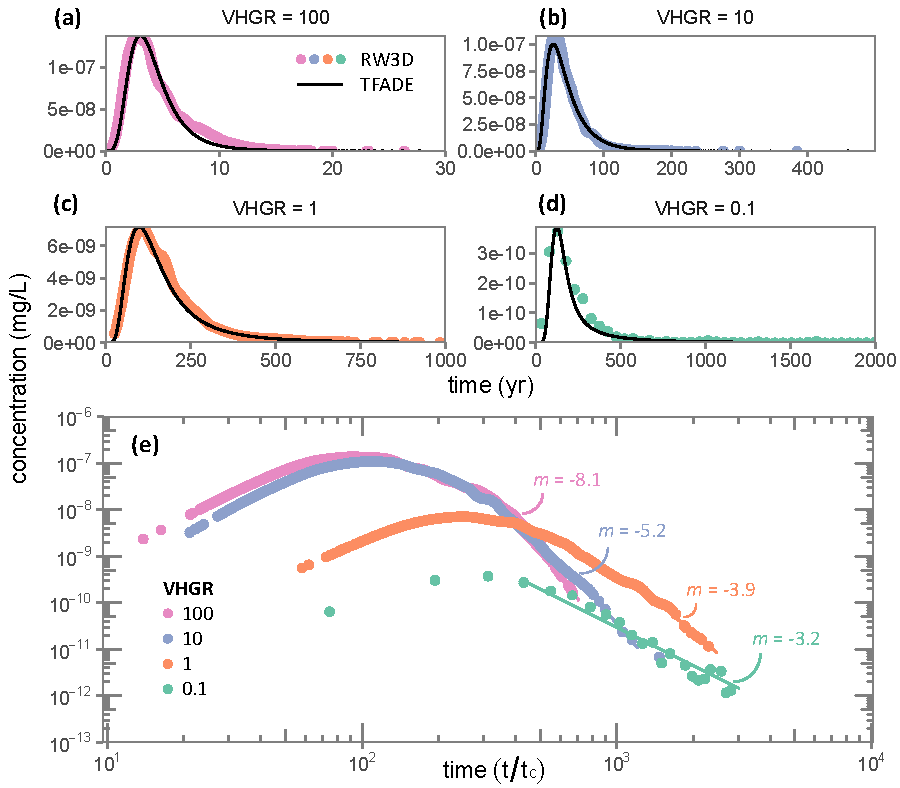
\includegraphics[width=\textwidth]{ch4_figs/tfade.pdf}
	\caption{(a-d) RW3D breakthrough curves (colored points) and fitted TFADE models (black line) measured at the bottom face of the domain (Figure \ref{fig:model}) for the four VHGR scenarios. Note the difference in x-axis travel times. (e) Breakthrough curves are normalized by the characteristic travel time (see SI Appendix Table \ref{ap_c_tc} for details). Measured slopes of tails (denoted as $m$) increase as VHGR decreases, corresponding to increasingly anomalous transport.}
	\label{fig:tfade}
\end{figure}



%
%----------- MSD ---------------%
%
\subsection{Temporal evolution of the plume spatial variance}
\label{ss_3_2}

Temporal evolution of the centered second spatial moments (Equation \ref{eq:msd}) in the longitudinal and transverse directions are superdiffusive and non-Fickian at early times across all VHGR scenarios; late time transitions either remain persistently preasymptotic, or revert to Fickian scaling, depending on the hydraulic gradient conditions (Figure \ref{fig:msd}). We now summarize spreading in the three directions:


\subsubsection{Longitudinal spatial variance}
\label{ss_3_2a}
The magnitude of longitudinal spatial variance (Figure \ref{fig:msd}a) increases with decreasing VHGR, and is preasymptotic and non-Fickian after 32 characteristic times for VHGR = 10, 1, and 0.1. In contrast, when VHGR = 100, late time longitudinal spreading is asymptotic and nearly Fickian ($\phi = $ 0.95 ). Spatial plume variance is around 4 orders of magnitude greater for VHGR = 0.1 compared to VHGR = 100 at all times. This large difference in the scale of spreading results in a wider-ranging residence time distribution between the scenarios (Figure \ref{fig:bottom_yx}a). A strong vertical hydraulic gradient when VHGR = 100 forces particles through nearly all facies in the downward, longitudinal direction (perpendicular to bedding layers), effectively generating an ergodic sample of the system heterogeneity much more rapidly than in scenarios with lower VHGR, thus late time spreading becomes in more Fickian nature. By contrast, at low VHGR, some of the plume remains trapped in fines, and some spreads longitudinally along preferential pathways--both of which stretch the plume.

% F:\Box Sync\Research\Post QE Research\DISSERTATION\02_ade\code/01_msd.R creates msd_time_2amean_ta1.pdf
% which is edited in AI in 02_ade/results/ msd_time_2amean_ta1_ai.pdf
\begin{figure}[H]
  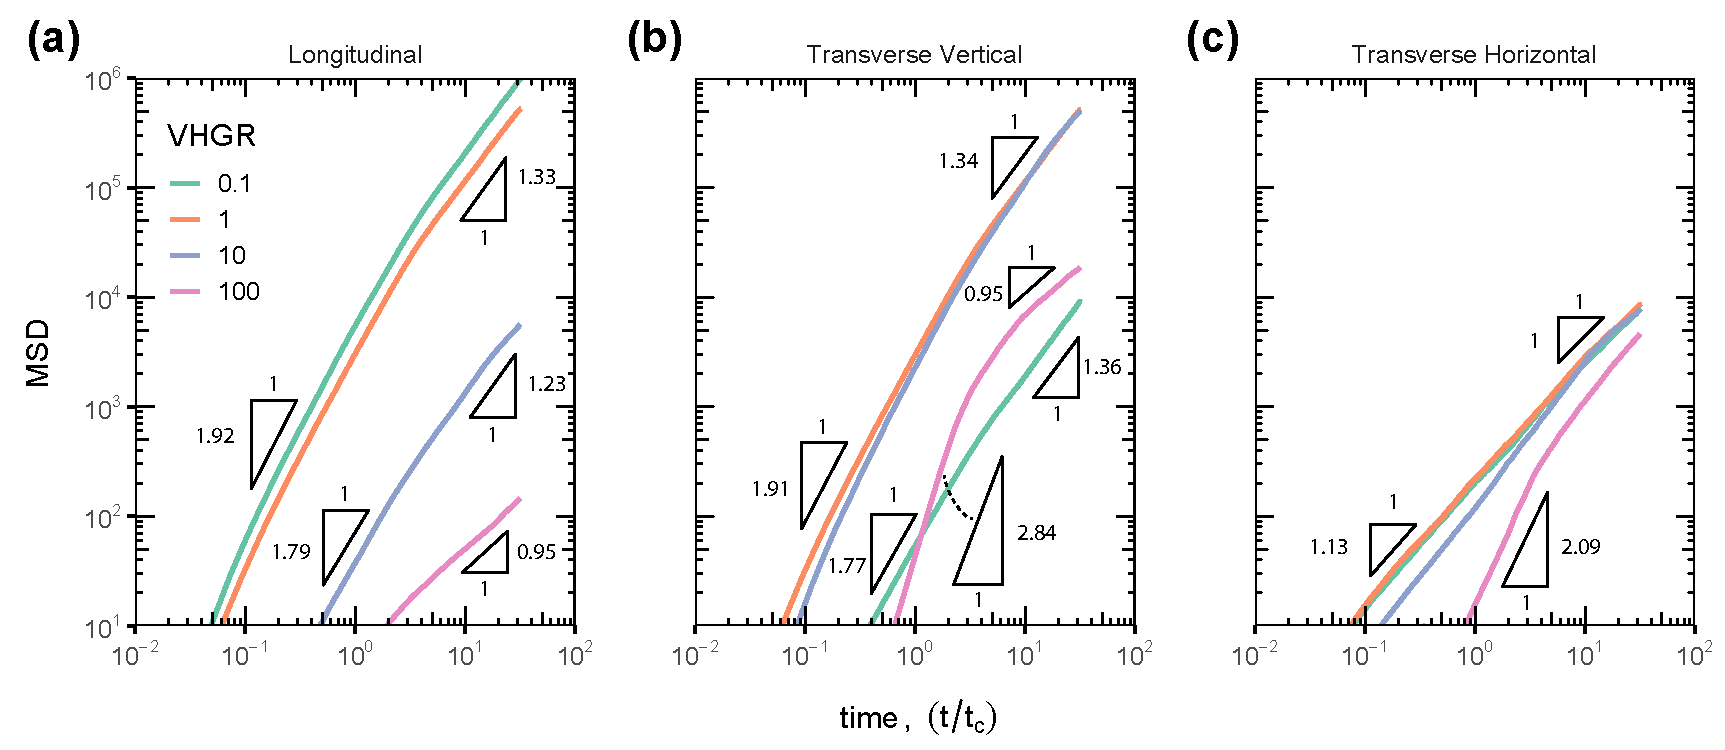
\includegraphics[width=\textwidth]{ch4_figs/msd_time_2amean_ta1_ai.pdf}
  \caption{Temporal evolution of the centered second spatial moments (Equation \ref{eq:msd}) calculated from the distribution of particle trajectories along the (a) longitudinal, (b) transverse vertical, and (c) transverse horizontal directions indicate superdiffusive early time scaling that reduces to less superdiffusive or Fickian scaling in late times, depending on the VHGR and direction of scaling. Triangles at early and late times show the slope of MSD temporal scaling, $\phi$ (Section \ref{ss_msd}).}
  \label{fig:msd}
\end{figure}


\subsubsection{Transverse vertical spatial variance}
\label{ss_3_2b}
Like longitudinal spreading, transverse vertical spreading (Figure \ref{fig:msd}b) in VHGR = 100 differs between the other three VHGR scenarios. VHGR = 100 is ballistic (i.e., $\phi >$ 2) at early times ($\phi$ = 2.84) due to entirely advection dominant facies (Table \ref{tab:model_l_k_pe}) and strong lateral connectivity of a high-K incised valley fill (Figure \ref{fig:ivf_xz}a) in the transverse vertical direction that facilitates preferential flow (discussed further in Sections \ref{ss_3_4} and \ref{ss_4_2}). However this spatial variance slows to nearly Fickian spreading ($\phi$ = 0.95) at late times. By contrast, VHGR = 10, 1, and 0.1 are super diffusive at early times (1.77 $\leq \phi \leq$ 1.91) but remain persistently preasymptotic and superdiffusive (1.34 $\leq \phi \leq$ 1.36) at late times rather than reverting to Fickian scaling as in VHGR = 100. 

The smaller magnitude of transverse vertical spatial variance observed when VHGR = 100 and 0.1 is explained by plume interactions with aquifer heterogeneity. When flow is vertical and downward (VHGR = 100), transverse transport is horizontal, tends to occur along extensive preferential pathways, and is driven toward these pathways by a powerful vertical gradient and all advection dominant facies. When flow is horizontal (VHGR = 0.1), transverse vertical transport is limited by diffusion dominant, laterally extensive paleosols and muds, which prevent spreading along this direction. The middle scenarios (VHGR = 1 and 10) by contrast have stronger vertical gradients to move particles past the first laterally extensive low-K layers, and then a combination of advection, slow advection, and diffusion dominant facies, which creates in greater transverse vertical spreading. 

The smaller magnitude of transverse vertical spatial variance observed when VHGR = 100 and 0.1 compared to VHGR = 10 and 1 is explained by plume interactions with aquifer heterogeneity. When flow is vertical and downward (VHGR = 100), transverse vertical transport occurs along the $y$ direction, which due to relatively high $K'_y$ compared to $K'_z$ should facilitate rapid spreading. However because all facies are advection dominant (Table \ref{tab:model_l_k_pe}) under the influence of powerful vertical gradients, particle trajectories tend to move relatively straight down along non-tortuous particle trajectories. For a different reason, when flow is horizontal (VHGR = 0.1), transverse vertical transport is limited by diffusion dominant, laterally extensive paleosols and muds, which prevent spreading along this direction. The middle scenarios (VHGR = 1 and 10) have a combination of advection, slow advection, and diffusion dominant facies, which simultaneously hold some mass back, and also move particles through laterally extensive low-K facies and layers, all of which results in relatively greater transverse vertical spreading. 


\subsubsection{Transverse horizontal spatial variance}
\label{ss_3_2c}
The absence of a gradient in the transverse horizontal direction (Figure \ref{fig:msd}c) limits superdiffusive early time scaling (1.13 $\leq \phi \leq$ 2.09), and leads to late time asymptotic Fickian scaling ($\phi$ = 1) after 32 characteristic times across all VHGR scenarios. We suspect that transverse horizontal early time superdiffusive scaling when VHGR = 100 is related to the same processes that create early time superdiffusive transverse vertical spreading: migration into preferential pathways. However, since the mean lengths of gravels (and the incised valley fill) in the transverse horizontal $x$ direction are less than in the transverse vertical $y$, the slope of early time superdiffusion is also less.  

In all directions and across all VHGR scenarios tested in this study (except for the VHGR = 100 in the longitudinal direction), superdiffusive early time scaling becomes more Fickian in late times as particles explore more of the system space, and hence the transport is increasingly ergodic. When VHGR = 100, late time longitudinal and transverse second moments approach Fickian scaling (rather than remaining persistently asymptotic), which suggests that an advection dominant system with powerful vertical hydraulic gradients can have a homogenizing impact on the anomalous transport created by system-scale heterogeneity. Furthermore, it illustrates how the degree of non-Fickian effects created when the mean flow direction changes (e.g., persistent superdiffusive scaling) may challenge upscaled approaches that currently fail to capture non-Fickian effects under similar boundary condition transience \citep{guo2020adaptive}.



%
%----------- Influence of preferential flow ---------------%
%
\subsection{Influence of geology on preferential flow and tailing}
\label{ss_3_4}

Non-Fickian transport is influenced by geologic heterogeneity in the hydrofacies model, including a high-K, interconnected incised valley fill, laterally extensive low-K paleosols, and the large volume fraction of low-K mud that plays an important role in diffusion and slow advection dominant transport.

The incised valley fill runs the laterally along the $y$ direction, and interconnects to an exit on the down-gradient side of the domain (Figures \ref{fig:ivf_xz}a-b). As VHGR decreases, particles take increasingly horizontal trajectories, and the incised valley fill and other interconnecting sand and gravel lenses act as a conduit for preferential flow that cause more particles exit the down-gradient side of the domain (Figures \ref{fig:ivf_xz}d,f,h,j), where they form clusters around gravel and sand facies (Figure \ref{fig:ivf_xz}b). Across all VHGR scenarios, particle trajectories that exit via the incised valley fill on the down-gradient side tend to exit at earlier timescales compared to other particles that exit the down-gradient side (lighter colored dots in the black oval compared to darker colored dots without outlines in Figures \ref{fig:ivf_xz}c,e,g,i), and compared to particles that take longer flowpaths and exit the bottom of the model at late times (darker colored dots in Figures \ref{fig:bottom_yx}c,e,g,i).

Notably, even at VHGR = 100 when most particle trajectories take vertical paths and exit the bottom face of the domain (yellow points in Figure \ref{fig:bottom_yx}d), some particles rapidly migrate in the transverse vertical direction along the incised valley fill to exit the down-gradient side (purple dots in the black oval in Figure \ref{fig:ivf_xz}d). Moreover, early time arrival through the incised valley fill when VHGR = 100 (Figure \ref{fig:ivf_xz}c) suggests that transverse horizontal preferential flow still occurs along interconnected coarse facies even under strong vertical gradients, and explains the ballistic early time transverse vertical scaling ($\phi = $ 2.84) in this scenario (Figure \ref{fig:msd}b).

Laterally extensive low-K paleosols limit (Figure \ref{fig:ivf_xz}b) the vertical migration of particles, and create segmented breakthrough along the down-gradient side of the domain where particles tend to exit above or below paleosol layers, but rarely through them (Figures \ref{fig:ivf_xz}d,f,h,j).



% F:\Box Sync\Research\Post QE Research\DISSERTATION\02_ade\code/
% 03_residence_time_distribution.R creates R objects `p5` and `p6` which are saved as PDFs: rt_t_final_xz_t.pdf, rt_t_final_xz_y.pdf. These are combined with paraview files (front_face_ivf.png and front_face.png) in  C:\Users\rpauloo\Documents\GitHub\kings-river-fan-tprogs\paraview. The generating .pbsm files should also be in that directory.
% finally, these are all combined in 02_ade/results/krf_front_face_ivf.ai
\begin{figure}[H]
  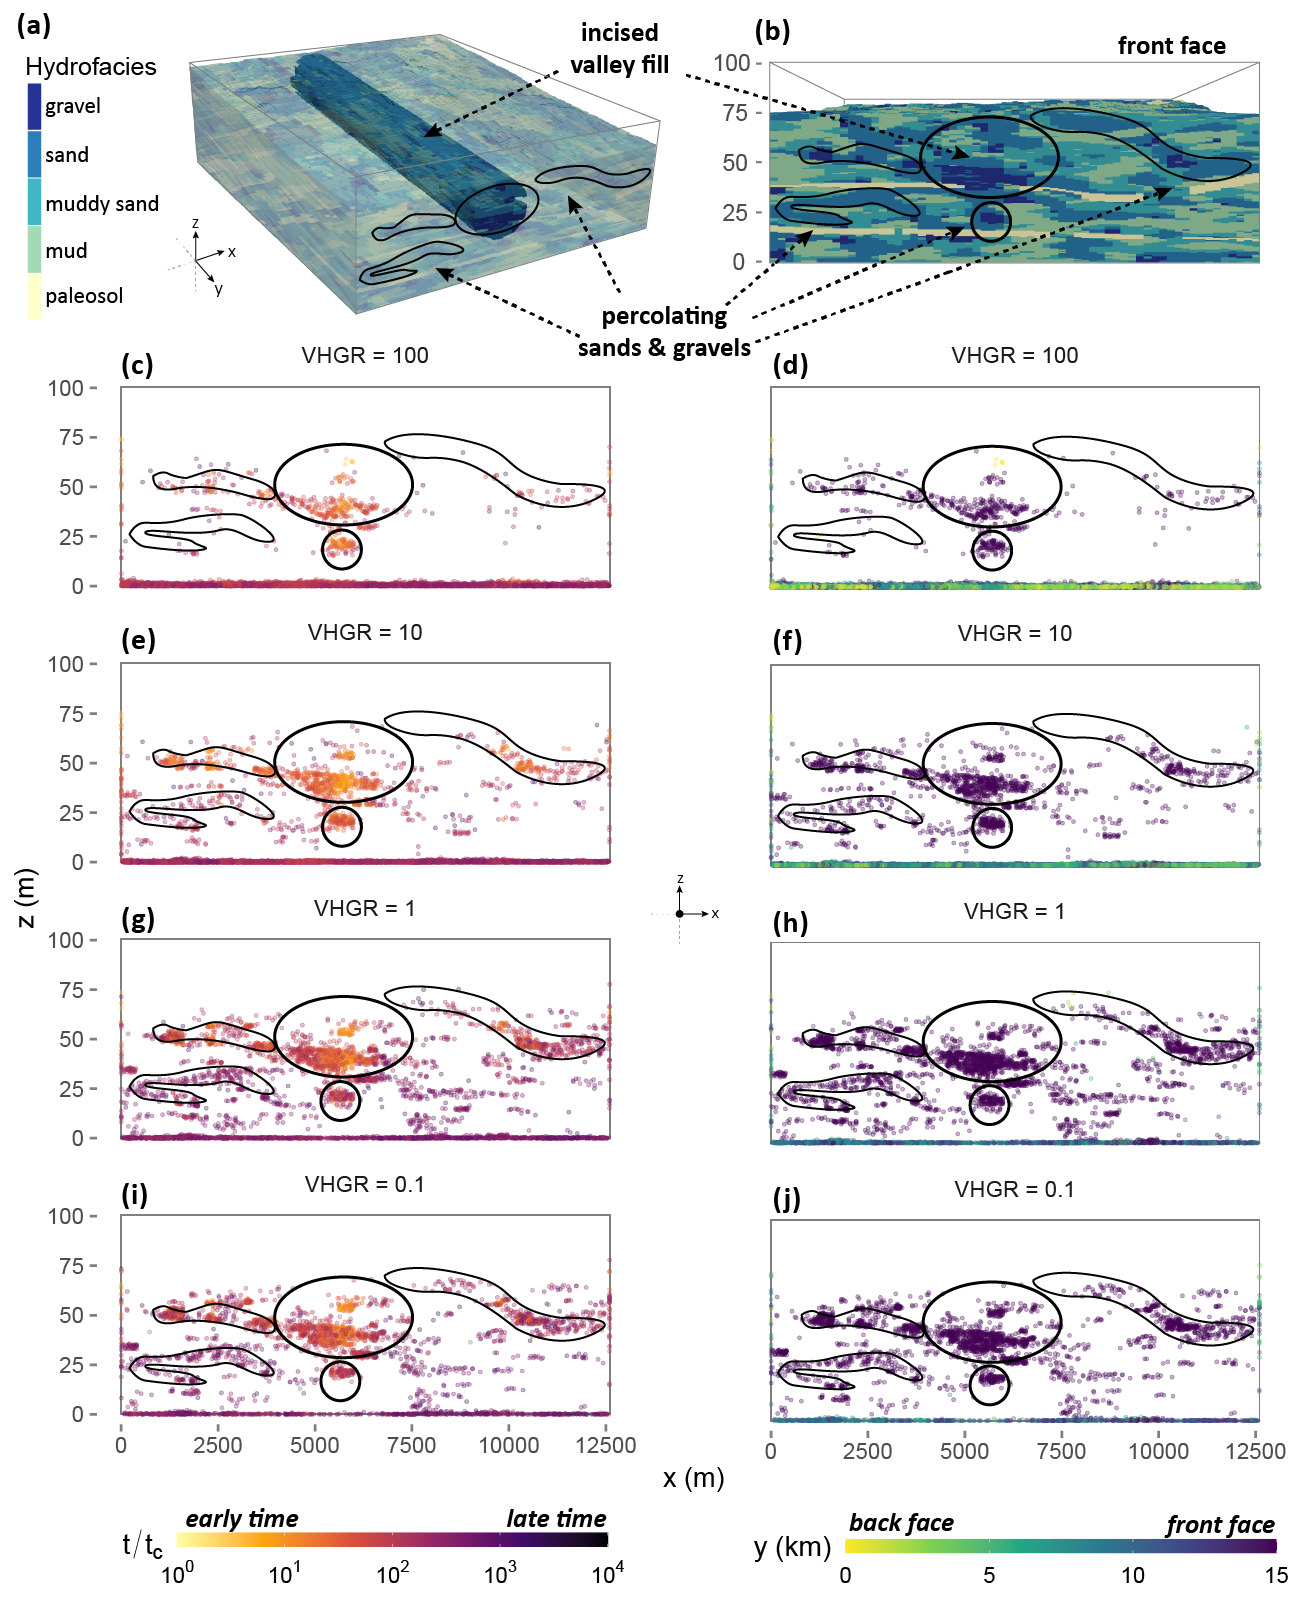
\includegraphics[width=\textwidth]{ch4_figs/krf_front_face_ivf_low_res-01.png}
  \caption{(a) Transparent 3D hydrofacies domain highlighting a lateral, interconnected sand and gravel incised valley fill; (b) The down-gradient side of the domain. A black oval marks the incised valley fill exit, and black outlines mark prominent interconnecting sands and gravel bodies that promote preferential flow. These same regions are marked in black in all other subplots; (c,e,g,i) The final $z$ and $x$ position of particles, colored by the time they exit the domain (residence time); (d,f,h,j) the final $z$ and $x$ position of particles, colored by the length ($y$) into the page, where yellow is the up-gradient side and purple is the down-gradient side. Particle clusters at $z =$ 0 $m$ indicate trajectories that exit the bottom face (Figure \ref{fig:bottom_yx}).}
  \label{fig:ivf_xz}
\end{figure}



% F:\Box Sync\Research\Post QE Research\DISSERTATION\02_ade\code/
% 03_residence_time_distribution.R creates R objects `p`, `p2`, `p3`, and `p4` which are saved as PDFs: rtd.pdf, rtd_inset.pdf rt_t_final_yx_t.pdf, rt_t_final_yx_z.pdf. 
% subplot (b) is made in /paraview/top_face.png and .pvsm
% finally, these are all combined in 02_ade/results/krf_top_face_rtd.ai
\begin{figure}[H]
  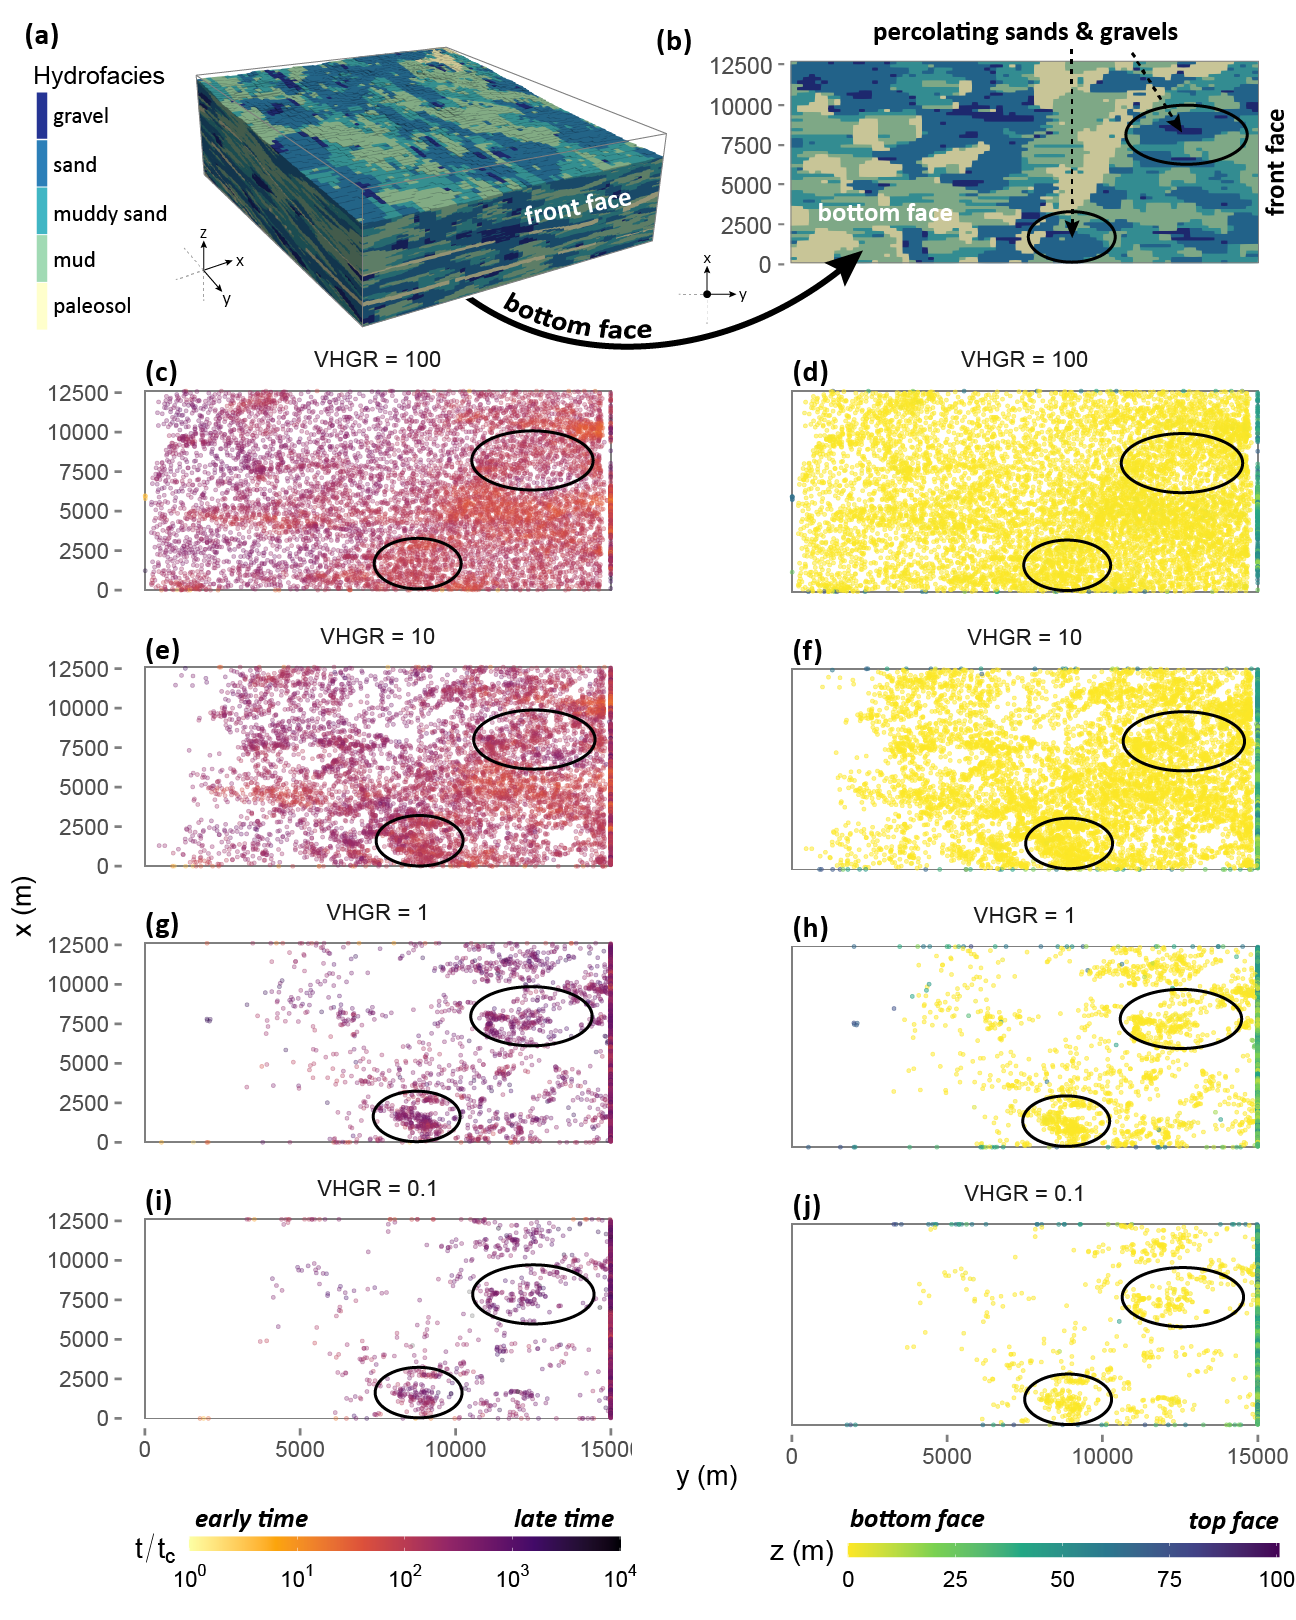
\includegraphics[width=\textwidth]{ch4_figs/krf_top_face_rtd_low_res-01.png}
  \caption{(a) The 3D hydrofacies domain; (b) the bottom of the domain with prominent sand and gravel bodies outlined in black; (c,e,g,i) the final $x$ and $y$ position of particles, colored by the time they exit the domain (residence time); (d,f,h,j) the final $x$ and $y$ position of particles, colored by the length ($z$) into the page, where yellow is the bottom face and purple is the top face. Particle clusters at $y =$ 15 000 $m$ indicate trajectories that exit the down-gradient side of the domain (Figure \ref{fig:ivf_xz}).}
  \label{fig:bottom_yx}
\end{figure}




%--------------------------------------------------------%
%	DISCUSSION
%--------------------------------------------------------%

\section{Discussion}

%
%----------- hydraulics ---------------%
%
\subsection{Mean flow direction modulates the degree of non-Fickian transport}
\label{ss_4_1}

In clastic sedimentary environments, significant vertical anisotropy in K and seasonal pumping and recharge can create strong vertical hydraulic gradients that in turn cause oscillations in mean flow direction. This study aimed to assess impacts of these shifting flow directions on the regional-scale, non-Fickian transport of nonpoint source contaminants in a typical alluvial aquifer-aquitard complex. Results demonstrate that shifting VHGR can \textit{modify the degree} of non-Fickian transport. Decreasing VHGR led to increasingly non-Fickian transport, measured by tailing at a control plane along the bottom face of the model, increased and persistent non-Fickian scaling of the second spatial moment, and increased preferential flow along interconnected high-K facies. 

Our results are consistent with previous studies which demonstrate that non-Fickian spreading measured (at a target well) can accompany the change from plume migration along an ambient groundwater gradient, to transient pump-and-treat conditions \citep{labolle2001role, guo2019upscaling, guswa2000slow}, which facilitates the release of mass stored in fine-grained material. Results illustrate that non-Fickian spreading of a nonpoint source plume depends on the mean flow direction, modified in many aquifer systems worldwide by ubiquitous pumping wells \citep{Famiglietti2014, Gleeson2012, wada2010global} that increase vertical head gradients and drive flow downward. 

Together, the increasingly non-Fickian effects (e.g., increased tailing, greater spatial spreading) that result as the mean flow direction shifts from horizontal to vertical suggest a conceptual model of nonpoint source transport in agriculturally intensive alluvial groundwater basins characterized by oscillating patterns of more Fickian vertical migration during periods of intense pumping and recharge, interspersed by periods of persistently non-Fickian lateral plume stretching under ambient groundwater flow when pumps are off and fields are not irrigated, except perhaps in areas with significant natural vertical anisotropy in K. These insights into the dependence of non-Fickian transport on mean flow direction bear importantly on efforts to model and manage nonpoint source contamination like salts \citep{hansen2018quantifying} and nitrates \citep{pasten2014assessment} in large irrigated basins where the flow boundary conditions (and hence VHGR) are inherently transient. Thus, an unresolved challenge for existing methods that upscale the advection-dispersion equation \citep{neuman2009perspective} is the ability to capture the varying non-Fickian behavior of regional, nonpoint source transport resulting from changes in the mean flow direction \citep{guo2020adaptive}. This study advances a hydrogeologic perspective towards understanding the physical genesis of this challenge.

%We emphasize that non-Fickian transport is driven by the interaction of hydraulics with well-characterized geologic heterogeneity. VHGR controls the ratio of advective to diffusive flux in hydrofacies (i.e., the Peclet number), and the mean flow direction, and hence the anisotropy encountered (i.e., flow parallel, perpendicular, or oblique to layers). Furthermore, results indicate that multiple scales of geologic heterogeneity (e.g., laterally extensive paleosols, a highly conductive incised valley fill) clearly influence plume-level non-Fickian transport, and hence, better characterization of multi-scale geology is imperative to modeling regional-scale transport \citep{zhang2006nonpoint}.



%
%----------- geology ---------------%
%
\subsection{Hydrogeologic heterogeneity underpins non-Fickian transport}
\label{ss_4_2}

Differing degrees of non-Fickian transport and plume spreading arise from hydrogeologic heterogeneity in the study site, which can be understood in terms of high ln-K variance, the transition from diffusion to advection dominant transport, and persistently non-Fickian transport caused by preferential flow and mass holdback.

%
%----------- ln K variance ---------------%
\subsubsection{The role of high ln-K variance}
\label{ss_4_2_1}

The geologically-based conductivity field in this study represents multi-scale heterogeneity, by which we mean multiple geologic sequences with large variance in K \citep{weissmann1999multi}, in contrast to stochastic Gaussian models with typical ln-K variances, $\sigma^2_{lnK} < $ 1 or 2 \citep{gelhar1993stochastic, rubin2003applied}. For our study site, $\sigma^2_{lnK} = $ 8.3, approximated by $\sigma^2_{lnK} \approx R^2/3$ \citep{fogg2016debates}, where $R$ is the range between the minimum and maximum values of K in orders of base 10 magnitude (i.e., 5 in this study).  Results suggest that non-Fickian transport is strongly affected by the transition of low-K facies along diffusion, slow advection, and advection dominated system states (Section \ref{ss_4_2_2}); and by the presence of an incised valley fill and laterally extensive, low-K paleosols (Section \ref{ss_4_2_3}). Furthermore, the persistently preasymptotic MSD scaling observed in some VHGR scenarios reinforce the notion suggested by other researchers \citep[e.g.][]{matheron1980transport, neuman1990universal, zhang2007persistence} that the late-time transition from non-Fickian to Fickian transport may never occur in natural geologic formations under certain gradient conditions. Thus, a key component to capturing non-Fickian effects is proper parameterization of the ln-K variance of the spatial heterogeneity.

%
%----------- Pe ---------------%
\subsubsection{Transitions between diffusion and advection dominant transport}
\label{ss_4_2_2}
In a spatial model with ln-K variance, transience in the hydraulic gradients can create systems that range from fully advection dominant, to systems of mixed advection and diffusion dominance, the latter of which will have greater non-Fickian effects.

As VHGR increases and flow is increasingly vertical, the hydrofacies Peclet number (Table \ref{tab:model_l_k_pe}) and hence advection dominant transport also increases. Importantly, in our study site, as VHGR increases from 0.1 to 100, the mud and paleosol facies shift from diffusion dominant ($P_e < $ 1) to slow advection and advection dominant ($P_e > $ 1). Consequently, high VHGR causes mass to migrate nearly straight through fines, consistent with the findings of \citet{guswa2000slow}, who observed accelerated solute release from low permeability zones under the influence of pumping in a slow-advection mass transfer system. In contrast to a diffusion dominant system, pumping would have little to no effect on the mass release from fines. Slow-advection is thus more related to the groundwater velocity, as opposed to a mass transfer model that strictly assumes diffusive controls on mass release from low permeability lenses. In this study, the decrease in non-Fickian transport observed at increasing VHGR and hence $P_e$ leads us to speculate that hydraulic forcings may exert a similar effect on transport as aquifer-aquitard spatial properties \citep[e.g.][]{zhang2006nonpoint, zhang2007predicting, yin2020super, zhang2013impact}. For instance, \citet{zhang2013impact} found that in domains containing hydrofacies with relatively short mean lengths, particles moved more rapidly between hydrofacies, which increased the likelihood for solutes to sample the full range of flow velocities, and thus more rapidly reach ergodicity. Similarly, we find that strong vertical flow (e.g., VHGR = 100) can push particles through all facies alike, thus accelerating mass transport between hydrofacies and rapidly reaching ergodicity. Furthermore, \citet{zhang2007predicting, zhang2013impact} observed that diffusion limited vertical floodplain layer thicknesses controlled late time non-Fickian solute tailing. Similarly, our results suggest that higher VHGR can shift facies from diffusion to advection dominance and diminish non-Fickian tailing. Hence, non-Fickian transport imparted by spatial heterogeneity should not be viewed as constant, but rather, as continually modified by hydraulic transience.

%
%----------- preferential flow and massholdback ---------------%
\subsubsection{Persistent non-Fickian transport}
\label{ss_4_2_3}

Describing persistent, late time, non-Fickian transport observed in this study (Section \ref{ss_3_2}) remains a modeling challenge. We now discuss the factors that control persistently preasymptotic non-Fickian transport, specifically how it relates to hydrofacies heterogeneity, preferential flow, and the transition from diffusion to advection dominant transport.

First, the super-linear growth of early time plume spatial variance observed in this study (i.e., superdiffusion, $\phi > $ 1) is consistent with other simulations in heterogeneous porous media \citep{zhang2013impact, kang2014pore, hunt2011dispersion}. The conventional understanding of this phenomenon is that preferential flow in highly permeable facies stretches the plume front downstream, while the trailing plume tail remains trapped by low-permeability facies near the source \citep{fiori2003flow, dagan2003flow, zhang2014linking, labolle2001role}. As ergodicity is reached in late times, plume spatial variance approaches Fickian scaling, which has been observed in numerous experiments \citep[e.g.][]{kang2014pore, le2010non, cortis2004numerical} and is relatively easier to model. However, persistently asymptotic behavior may never arise because the time needed to reach asymptotic behavior in natural geologic systems may be sufficiently large that the solute will encounter new spatial nonstationarities along the displacement distance before Fickian scaling is reached, and is thus always in a state of transition, never reaching asymptotic behavior \citep{matheron1980transport, gillham1984advection, neuman1990universal}.

We speculate that the multiple-scale geologic heterogeneity in our study area causes persistently non-Fickian superdiffusion at late times in longitudinal and transverse directions for all VHGR $\leq$ 10. This persistent late time non-Fickian transport is supported by \citet{labolle2001role}, who noted persistent preasymptotic ambient transport in a similar well-connected, hydrofacies-based alluvial fan model. Moreover, \citet{zhang2007persistence} found that transition times in simple, 2D uniform media were so large, that the authors speculated that in natural geologic media with multiple‐scale heterogeneity, the transition from anomalous to Fickian transport may never complete. Complimentary to these observations, our results indicate that sufficiently high VHGR can reduce the impact of mass sequestration in fines, lead to a more compact plume in all directions, and hence, promote asymptotic late time Fickian scaling in all dimensions, thus lending itself towards being more appropriately described by an upscaled model.  

The important role of preferential flow on persistent non-Fickian transport is illustrated by the impact of a lateral, connected, incised valley fill and other prominent interconnecting sand and gravel bodies (Figure \ref{fig:ivf_xz}a). When VHGR = 100, rapid particle migration into the incised valley fill transverse vertical to the mean flow direction resulted in early time hyper-ballistic scaling ($\phi = $ 2.84) of transverse vertical MSD that slowed to nearly Fickian scaling ($\phi = $ 0.95) at late times as ergodicity was reached. In contrast, when VHGR = 10, 1, and 0.1, preferential flow along high-K networks stretched some of the plume at the same time that fines sequestered other parts of it, leading to persistent and oftentimes a greater magnitude of late-time spreading ($\phi = $ 1.34 - 1.36). Across all scenarios, particles traveled laterally through the incised valley and exited the down-gradient side at relatively earlier times (Figure \ref{fig:ivf_xz}c). Observations of faster transport along highly-permeable, interconnected sand and gravel lenses are consistent with numerous studies of preferential flow \citep{winograd1976major, jussel1994transport, moreno1994flow, tsang1998flow, fogg1986groundwater, heeren2010preferential, maxwell2008contamination, zheng2003analysis, weissmann2004influence, labolle2001role}. 

Final particle positions and the hydrofacies they occupy at that time further illustrate the importance of advection and diffusion dominant transport and preferential flow. When VHGR = 100 and advection dominates transport, particles are nearly indiscriminate in terms of the facies they occupy upon exiting the bottom face of the domain (i.e., even spatial distribution of yellow dots in Figure \ref{fig:bottom_yx}d). By contrast, when VHGR = 0.1, spatial patterns of particles that exit the bottom face of the domain (yellow dots in Figure \ref{fig:bottom_yx}j)) and the down-gradient side (purple dots in Figure \ref{fig:ivf_xz}j) correlate with more conductive, high K facies (blue and dark blue sand and gravel in Figures \ref{fig:bottom_yx}b and \ref{fig:ivf_xz}b). This indicates preferential flow along interconnecting sand and gravel lenses, and partly explains the increased non-Fickian transport with decreasing VHGR as a result of relatively rapid plume stretching along these fast flowpaths. 

%Surprisingly, VHGR = 0.1 and 100 exhibit a more similar magnitude of transverse vertical MSD, even though the mean flow directions in these scenarios were the most extreme tested in this study, ranging from mostly horizontal to mostly vertical. However, this seemingly counter-intuitive finding can be reconciled by considering the interaction of mean flow direction, the spatial heterogeneity of the domain, and the role of advection and diffusion dominant hydrofacies on transport. When VHGR = 100, particle trajectories move nearly straight down (Figure \ref{fig:res_time_dist_yx}d), even migrating through laterally extensive low-K hydrofacies, which under the influence of strong gradients become advection dominant (Table \ref{tab:model_l_k_pe}), thus helping to facilitate this vertical transport. 
%The temporal evolution of the hydrofacies proportions support these observations, and show higher paleosol occupancy for high VHGR, and advection-driven mass transfer out of paleosols (Figure \ref{fig:phft}). 
%For a different reason, we observe similar scaling of the transverse vertical MSD when VHGR = 0.1. In this case, flow is more horizontal and parallel to the bedding layers, but the transverse vertical mass transfer is limited by abundant, laterally extensive, and muds and paleosols which are diffusion dominant at these hydraulic gradients (Table \ref{tab:model_l_k_pe}), which prevents mixing along the transverse vertical direction, and thus limits the magnitude of transverse vertical MSD scaling. By contrast, plumes in the intermediate scenarios (VHGR = 1 and 10) exhibit a greater magnitude of transverse vertical spreading. In these scenarios, vertical hydraulic gradients are sufficiently large enough to drive vertical transport, and the mud and paleosol hydrofacies can be advection dominant, which increases transverse mass exchange along these facies, and thus the plume spreads more in the transverse vertical direction.



%
%----------- upscaled models ---------------%
%
\subsection{Implications for upscaled transport models}
\label{ss_4_3}

The varying degrees of non-Fickian transport that arise from the interaction of hydraulics and geologic heterogeneity challenge the application of the advection-dispersion equation towards subsurface transport problems in natural geologic media. At regional scales (e.g., tens to hundreds of kilometers), subsurface characterization may be intractable or cost-prohibitive, and even if reliable subsurface models were available, the computational complexity of solving transport over these scales would be enormous. Hence, regional upscaled transport models are needed. These upscaled models must be able to represent non-Fickian effects created by preferential flow in connected high‐conductivity facies, mass transfer processes between high‐ and low‐conductivity media, and as we show in this study, the different degrees of non-Fickian transport introduced by changes in the mean flow direction due to varying VHGR (e.g., in the case of significant pumping and recharge).

In a previous study, \citet{guo2020adaptive} demonstrated an adaptive multirate mass transfer (aMMT) model which improved breakthrough curve estimation for diffusion dominant transient flow by incorporating time-dependent mass transfer coefficients based on the equivalent flow velocity. However, the aMMT approach failed to capture tailing in breakthrough curves when the mean flow direction changed, as in the case of shifting VHGR. In this study, we extend the work of \citet{guo2020adaptive} and illustrate that as VHGR changes, the transition from diffusion to slow advection and advection dominance in the discrete hydrofacies of a system can fundamentally change the mass transfer processes. Specifically, high VHGR (provided it creates system-wide advection dominance) can cause solutes to move nearly straight through facies (e.g., Figures \ref{fig:model} \ref{fig:bottom_yx}d even though the vertical effective K is much less than the horizontal effective K, whereas low VHGR (diffusion to slow advection dominance some facies) can lead to mass holdback in fines (Figure \ref{fig:tfade}) and strong preferential flow (Figures \ref{fig:ivf_xz}h,j and \ref{fig:bottom_yx}h,j). Thus, a future promising direction towards the goal of improving estimation of late time tailing under transient flow is to quantify changes in VHGR, $P_e$, mean flow direction, and characteristic length scales along the mean flow direction, and relate these to mass transfer processes parameters in a upscaled model (e.g., aMMT).




%
%----------- limitations ---------------%
%
\subsection{Study limitations and additional considerations}
\label{ss_limitations}

We explore highly detailed nonpoint source plume evolution across a series of steady state flow simulations in order to observe regional-scale, long term transport under conditions that represent the transition from relatively ambient groundwater flow to predominantly vertical flow. However, these steady state simulations do not the capture mass transfer effects that occur when hydraulic boundary conditions rapidly change, as in the case of a pumping well being turned on. For example, \citet{bastani2020effects} found that transport models based on steady state flow did not capture short-term oscillations of nitrate concentrations in pumping wells at the local scale. Similarly \citet{guo2020adaptive} showed that the aMMT model failed to reproduce transport when the flow direction changed, and \citep{labolle2001role} observed the release of mass stored in fine-grained material when boundary conditions changed from plume migration along an ambient groundwater gradient, to transient pump-and-treat conditions. Thus a future challenge is to explore nonpoint source plume evolution in a transient simulation that incorporates transitions between each VHGR scenario, and which represents the hydraulic conditions observed in natural irrigated basins with extensive pumping. 

Heterogeneous porous media affects reactive solute transport by controlling solute mixing and residence times \citep{perez2019organic}, which may be more important for certain solutes and depth zones. In this study, we simulate a nonreactive solute, which may not be suitable for some nonpoint source contaminants in fully saturated groundwater. More research needed on how reaction rates may alter the non-Fickian effects explored in this study, for instance, by mineral dissolution of the domain which adds a source term \citep{schoups2005sustainability}, or in the case of nitrates, by denitrification in the soil zone \citep{lee2006nitrogen}. 

It is well known that hydrofacies geometry influences contaminant transport, and hence, our study is best interpreted with respect to the characteristic geology of the domain. For example, \citet{yin2020super} found that larger hydrofacies width increased high-permeability connectivity, and thus superdiffusion; conversely, larger mean hydrofacies thickness slowed solute migration and reduced plume scaling. Any extrapolation the results presented herein to other areas should be accompanied by a careful consideration of the hydrogeology of the new study site.



%--------------------------------------------------------%
%	CONCLUSIONS
%--------------------------------------------------------%
\section{Conclusions}
\label{s_5}


We simulated 3D steady state groundwater flow and nonpoint source contaminant transport in a regional scale (15 $km$ x 12.6 $km$ x 100 $m$) geostatistical representation of a heterogeneous alluvial aquifer-aquitard system. In horizontally stratified clastic sedimentary aquifer systems it is common for the strong vertical anisotropy of hydraulic conductivity to produce spatially and temporally varying vertical and horizontal components of the hydraulic gradient, in turn producing a complex interplay between the stratified heterogeneity and physical transport processes. These effects can be augmented and made highly transient by the effects of pumping and recharge in, for example an agricultural system where oscillations between primarily horizontal and primarily vertical flow are caused by seasonal fluctuations in pumping as well as the recharge produced by irrigation. Thus we tested the impact of these varying mean flow directions on non-Fickian transport, and observed increasingly non-Fickian transport as flow was increasingly horizontal (i.e., when the VHGR decreased). Importantly, when VHGR was large (e.g., 100), the plume was more compact: particle trajectories exhibited late time asymptotic Fickian scaling of spatial variance, and moved perpendicular to the direction of aquifer bedding (even though the vertical effective K is much less than the horizontal effective K), and nearly straight through high- and low-conductivity facies alike. As VHGR decreased (e.g., 10 and 1) flow became more horizontal and transport was more non-Fickian -- particle trajectories increasingly moved along laterally extensive facies, took preferential flowpaths, and exhibited greater (and preasymptotic) spatial spreading and tailing in breakthrough measured along a control plane at the bottom face of the model. Hence, the non-Fickian transport imparted by spatial heterogeneity should not be viewed as constant, but rather, as continually modified by hydraulic transience that may transition facies from diffusion to advection dominance and thus alter non-Fickian mass transfer dynamics. These results illustrate why conventional methods to upscale anomalous transport under transient flow conditions remains a challenge, and indicates that future efforts to upscale regional-scale, transient nonpoint source transport may benefit by incorporating information on the time-dependent changes in VHGR, $P_e$, mean flow direction, and characteristic length scales along the direction of mean flow.



 %This looks for chapter4.tex
%%%%%%%%%%%%%%%%%%%%%%%%%%%%%%%%%%%%%%%%%%%%%%%%%%%%%%%%%%%%%%%%%%%%%%%%%%%%
\section{Supporting Information Appendix} \label{ap_c_vhgr}


\subsection{Simulated groundwater head for VHGR scenarios}

\begin{figure}[H]
\label{ap_c_heads}
  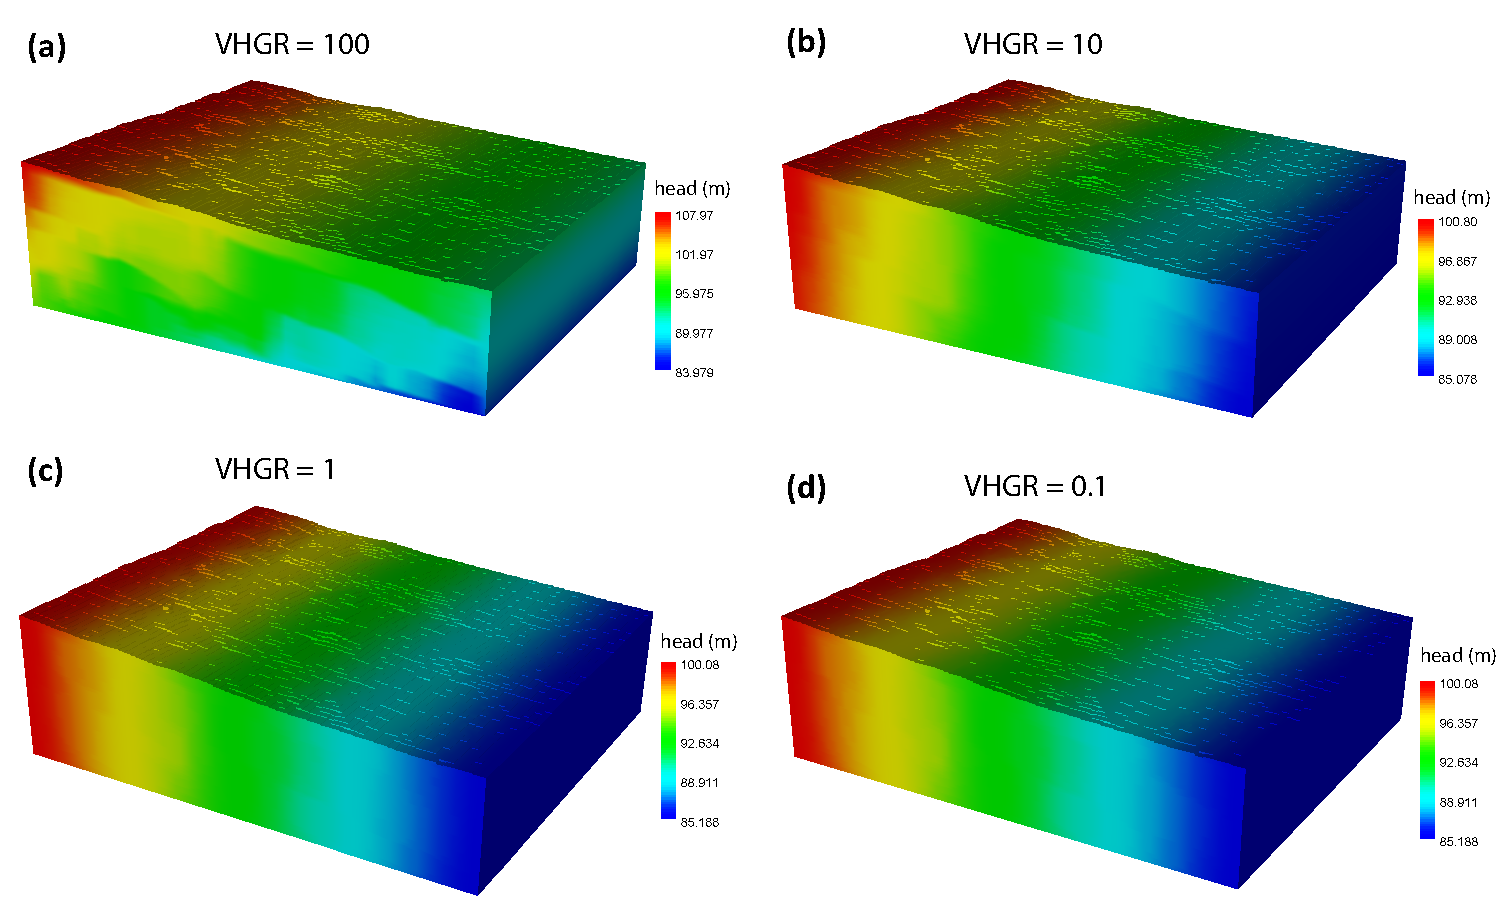
\includegraphics[width=\textwidth]{ch4_appendix_figs/heads.pdf}
  \caption{(a-d) Simulated steady state groundwater head across the 4 VHGR scenarios tested in this study.}
  \label{ap_c_heads_vhgr}
\end{figure}



%--------------------------------------------------------%
\subsection{Particle trajectory coordinate rotation and travel time normalization via the characteristic travel time}
\label{s_ap_c_part_rot}

In order to ensure comparability across the range of VHGR scenarios of differing travel times and mean flow direction, we perform coordinate rotations and normalize travel times by a characteristic travel time to travel the average facies length, $t_c$. 

First, we compute the mean Lagrangian velocity across all trajectories, $\bar{v}$ and use the characteristic time to travel the average facies length, $t_c$, to normalize time across VHGR scenarios (SI Appendix Table S1). The mean velocity and facies length are calculated along the direction of mean flow. Since this direction varies across VHGR, by an angle $\Phi$ relative to the horizontal direction, and the model outputs trajectories in a regular 3D Cartesian grid, we rotate the particle trajectory coordinates about the $x$ axis by $\Phi$ to recover the the transformed $y$ and $z$ components along the longitudinal and transverse vertical directions respectively ($y’$ and $z’$):

\begin{equation}
\begin{aligned}
\label{eq:rotation}
    y' = z \cdot sin(\Phi) + y \cdot cos(\Phi) \\
    z' = z \cdot cos(\Phi) - y \cdot sin(\Phi)
\end{aligned}
\end{equation}

Flow occurs along $zy$, thus the $x$ coordinates (transverse horizontal) remain unchanged. After transforming coordinates according to (\ref{eq:rotation}), we calculate longitudinal displacement along $y’$, transverse vertical displacement along $z’$, and transverse horizontal displacement along $x$.



\bgroup

\renewcommand{\arraystretch}{1.5}

\setlength{\tabcolsep}{20pt}

\begin{table}[H]

\caption{Mean velocity $\bar{v}$ along the longitudinal direction ($y'$), the angle of mean flow, relative to the horizontal direction in the un-rotated Cartesian coordinate system $\Phi$, the characteristic hydrofacies length $\lamdba_c$ along the longitudinal direction, and the characteristic time $t_c$ along the longitudinal direction ($t_c = l_c / \bar{v}$).} 
\centering


\begin{tabular}{lrrrr}
\label{ap_c_tc}

\textbf{VHGR} & $\bm{\Phi} (^{\circ})$ & $\bm{l_c \: \: (m)}$ & $\bm{\bar{v} \: \: (m/yr)}$ & $\bm{t_c \: \: (yr)}$  \\ 
\hline
   100 & 89.43 & 2.19  & 73.33 & 0.046 \\
   10  & 84.29 & 2.20  & 8.40  & 0.252 \\
   1   & 45.00 & 3.09  & 7.20  & 0.093 \\
   0.1 & 5.71  & 21.97 & 53.01 & 0.319 \\
\hline
\end{tabular}

\end{table}
\egroup




%--------------------------------------------------------%
\subsection{RW3D parameters}


% 01_mm_plots_tables.R in F:/ ... POst_QE_Research/DISSERTATION/01_mm
% search for gw_and_sw_c_summary table


\bgroup

\renewcommand{\arraystretch}{1.5}

\setlength{\tabcolsep}{20pt}

\begin{table}[H]

\caption{RW3D parameters for each VHGR scenario including the number of injected particles (particle count), the maximum simulation time (max time), and the number of snapshots saved (snapshot count). Note that the snapshot count = max time $\cdot$ 10 000, meaning that for each scenario, 100 snapshots were taken per year of simulation time.} 
\centering

\begin{tabular}{lrrr}
\label{ap_c_rw3d_params}

\textbf{VHGR} & \textbf{particle count} & \textbf{max time (yrs)} & \textbf{snapshot count}  \\ 
\hline
   100 & 10 000  & 100   & 10 000  \\
   10  & 10 000  & 500   & 50 000  \\
   1   & 10 000  & 1000 & 100 000 \\
   0.1 & 10 000  & 5000 & 500 000 \\
\hline
\end{tabular}

\end{table}
\egroup








%--------------------------------------------------------%
\subsection{Hydrofacies proportions over time}



\begin{figure}[H]
  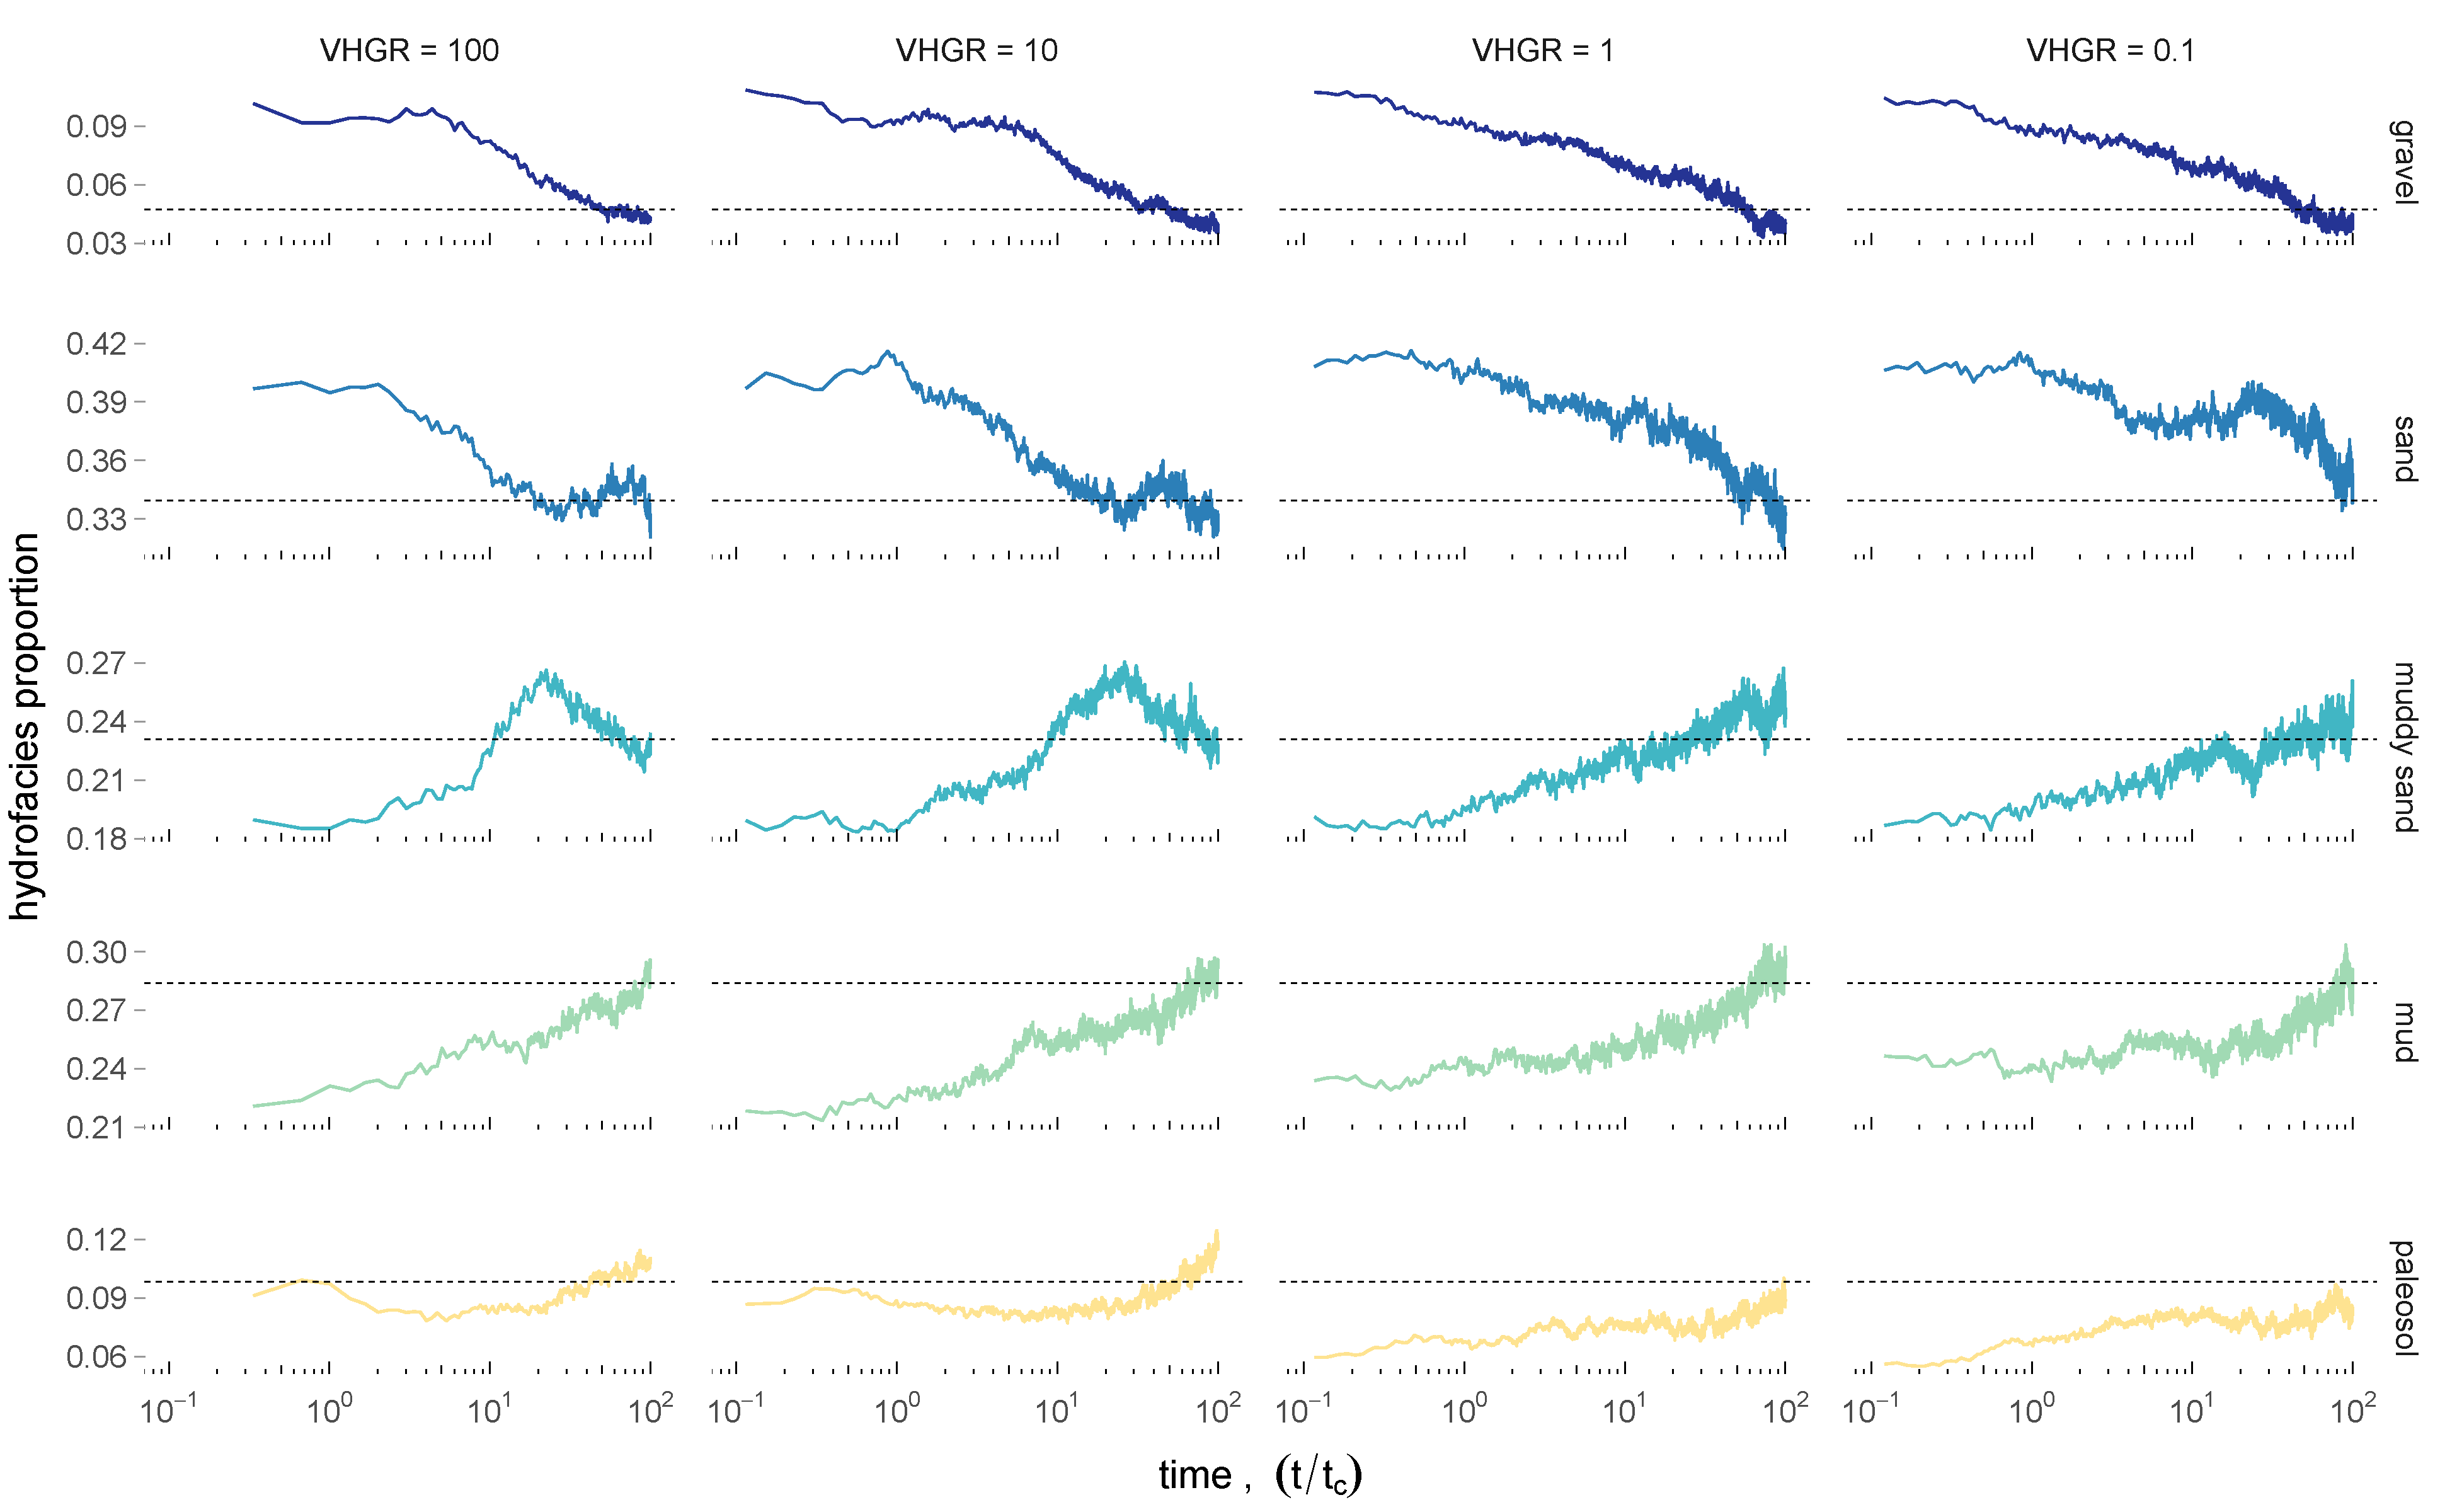
\includegraphics[width=\textwidth]{ch4_appendix_figs/phf_over_time_00_03_ai.pdf}
  \caption{Proportion of hydrofacies occupied by the particles as a function of time across the 4 VHGR scenarios indicate mixing: over about 32 characteristic times, proportions converge onto the hydrofacies proportions shown as black, dashed horizontal lines. Note the difference in y axis between the rows, each of which correspond to a distinct hydrofacies..}
  \label{ap_c_heads_vhgr}
\end{figure}



\clearpage



%--------------------------------------------------------%
% Acknowledgments
%--------------------------------------------------------%
\section{Acknowledgments}

We gratefully thank Drs. Yong Zhang, Marco Dentz, and Song Wei for their feedback and modeling advice. Support for this research was provided by the National Science Foundation (NSF) Climate Change, Water, and Society (CCWAS) Integrated Graduate Education and Research Traineeship (IGERT) program at the University of California, Davis (http://ccwas.ucdavis.edu, DGE-10693333), and by the U.S./China Clean Energy Research Center for Water-Energy Technologies (CERC-WET). %All data is accessible via Dryad at \textit{URL WITH DOI TO BE INPUT}, and procedures and models are accessible via Github at \textit{URL WITH DOI TO BE INPUT}.  




\clearpage
\printbibliography[heading=bibliography]

% chapter 5
%\chapter{Real Title Here}
\chapter[Concluding Remarks.]{Concluding Remarks}

Writing near the turn of the 21st century, Dr. Norman Borlaug, a Nobel Laureate and key figure in the Green Revolution credited with pivotal advancements in plant genetics, noted that the continued success of the Green Revolution depended on fresh water availability, and called for a ``Blue Revolution'' to secure reliable water resources. Civilization's reliance on unsustainable groundwater pumping, especially in clastic sedimentary groundwater basins found in arid and semi-arid regions worldwide, limits the lifespan of these freshwater stores \citep{Scanlon2012, wada2010global, Gleeson2012}. For example, in California's Central Valley, aquifer lifespan has been estimated at 390 years or less depending on the exact location and depletion rate \citep{Scanlon2012}. Although aquifer depletion poses a long-term existential threat, a range of negative consequences (e.g., land subsidence, surface water depletion, destruction of groundwater-dependent ecosystems) will impact surface and groundwater systems long before aquifer stores run dangerously low, and these impacts will be exacerbated by surface water shortages in a warming climate \citep{Rhoades2018, Swain2018, Cook2015}, which has historically increased groundwater pumping to augment lost surface water supply \citep{Hanak2011, Medellin-azuara2016}. Thus, by addressing the short term consequences of aquifer depletion, the larger and slower-moving existential threat of aquifer depletion is also mitigated. 

This dissertation focuses on the development of models to address two understudied consequences of aquifer depletion: well failure and closed basin salinization. Chapter 2 demonstrates how data assimilation from monitoring well networks and open data from state agencies can be combined into a physical model of well failure that forecasts the impact of extended drought duration, groundwater management regimes, and wet winter recharge events in California's Central Valley. Chapter 4 advances a conceptual model of Anthropogenic Basin Closure and groundwater SALinization (ABCSAL), and first-order estimates of salinization in California's Tulare Basin. Chapter 3 uses 3D numerical flow and transport modeling in a complex hydrofacis model to show that transience in the mean flow direction caused by naturally-occurring (due to natural anisotropy in K) and induced hydraulic gradient transience (from pumping and recharge) can change the governing mass transfer processes in hyrdofacies, leading to differing degrees of non-Fickian transport. 


Chapter 2 demonstrates the vulnerability of domestic wells to both naturally-occurring hydrologic events (e.g., drought and wet winter recharge) and human-made water management decisions (e.g., sustainable and business as usual management regimes). Results indicate that extended drought durations (e.g., 5 to 8 years) can lead to a greater annual rate of well failure than observed during historic droughts (e.g., 2012-2016) as groundwater levels intersect an increasingly dense portion of the distribution of domestic well pump depths. Moreover, human water management decisons matter. Four times as many wells failed--even when controlling for hydrologic uncertainty--between a strict sustainability scenario in which groundwater levels were not allowed to fall after 2020, compared to a business as usual scenario that projected current groundwater level decline trends into 2040. Wet winter recharge events, and hence reduced pumping \citep{Hanak2019} and flood-based managed aquifer recharge \citep{Kocis2017} show potential to lessen the degree of domestic well failure. Looking forward, as Internet-of-things technologies mature and remote sensor networks are increasingly cost-effective and easy to maintain, the real-time monitoring of groundwater \citep{calderwood2020low} will permit data-driven models like the one presented in this study to automatically assimilate real-time groundwater level data and provide on-the-fly well failure risk estimates. Thus, it is conceivable that an early warning system for domestic well failure--not unlike existing early warning systems for drought \citep{pozzi2013toward, huang2004drought}--may be a future possibility enabled by sensor technology and cloud computing.

Similarly to Chapter 2, the topic of Chapter 3 remains understudied due to its relatively new emergence. Chapter 3 explores a mechanism by which groundwater pumping eliminates hydrologic exits for naturally-occurring salts in a basin (e.g., via baseflow and lateral subsurface outflow), after which those entrained salts accumulate in shallow aquifers due recycling from pumping and irrigation, before they are driven into deeper aquifer over century-long timescales. We call this process Anthropogenic Basin Closure and groundwater SALinization (ABCSAL). Importantly, results from a first-order mixing cell model indicate that shallow aquifers reach drinking water minimum thresholds for total dissolved solids (TDS) within decades, a result consistent with measurements of shallow aquifer TDS increase in the past century in the study site \citep{Hansen2018}. These results suggest that one mechanism to reverse or slow ongoing ABSCAL may include ``filling the basin up'' with significant recharge to restore baseflow and lateral subsurface outflow. Although the practical reality of such a management action may be cost-prohibitive or physically limited by available surface water in the Tulare Basin, it remains a viable solution in other basins worldwide experiencing ABCSAL. Moreover, a greater emphasis on subsurface water storage will require tightly monitoring and managing the ground and surface water interactions with distributed sensor networks, in order to prevent capillary rise and salinization from bare soil evaporation \citep{belitz1995alternative}. Without these mitigative management actions, ongoing and long-term ABCSAL may require inland desalinization of pumped groundwater.

Building on the work presented in Chapter 3, Chapter 4 uses 3D numerical groundwater flow and transport simulations in a detailed hydrofacies model with large variance in K \citep{weissmann1999multi} to better understand how hydraulic transience in the mean flow direction influences the degree of non-Fickian transport observed in hydrogeologic systems (e.g., nonpoint source salts discussed in Chapter 2). In California's Central Valley and other typical clastic sedimentary alluvial aquifer-aquitard systems worldwide, high vertical anisotropy in K naturally created by the inter-bedding of high and low K sediments, combined with pumping and recharge, can create flow systems that oscillate between predominately vertical and horizontal flow. Although other studies have noted that classical methods to upscale transport fail to represent tailing when the mean flow direction changes \citep{guo2019upscaling, guo2020adaptive}, the hydrogeologic underpinnings of this phenomenon remain poorly understood. Results indicate that relatively higher vertical to horizontal gradient ratio (VHGR) coincident with increasingly vertical mean flow direction can transition low-K facies from diffusion- to advection-dominant, and cause vertical groundwater flow to move directly through facies that typically act as aquitards at lower VHGR (e.g., paleosols, clays, and silts). In other words, when systems transition from diffusion- to advection-dominant, non-Fickian behavior (e.g., tailing, spatial variance, preferential flow) all decrease. These results imply a conceptual model of oscillating patterns in the degree of non-Fickian transport that correspond to seasonal patterns of pumping and recharge. Hence, non-Fickian transport models will better characterize flow systems under higher VHGR, depending on the gradients, characteristic facies length scales, and the Peclet number ($P_e$) of the distinct hydrofacies which describes the ratio of advection to diffusion time scales. These results also suggest a physical mechanism for arsenic leeching from low-K clays observed in the Central Valley during periods of land subsidence \citep{smith2018overpumping}, driven by advective flushing as strong vertical gradients ``force'' groundwater through clays. Lastly, the strong dependence of mass transfer on hydrogeologic features illustrated in this study suggests that future efforts to upscale regional-scale, transient nonpoint source transport may benefit by incorporating information on the time-dependent changes in VHGR, $P_e$, mean flow direction, and characteristic length scales along the direction of mean flow.

Securing sustainable groundwater resources in the 21st century and beyond will require the further development and refinement of hydrogeologic science, and numerical and data-driven models to assimilate that understanding and provide critical insights. Although this dissertation focuses on groundwater problems in California, the themes explored herein are extensible to other heavily pumped groundwater systems worldwide. Indeed, it is only through enhanced understand of aquifers that civilization may bring about a Blue Revolution in groundwater resources monitoring, modeling, and management.

\clearpage %This looks for chapter5_conclusion.tex
\printbibliography[heading=bibliography]


% note that the 'plainnat' style does not allow URL's in the bibtex entry
%
% some ideas here:
% http://bib2web.djvuzone.org/bibtex.html
%

% reset the page style
%\pagestyle{plain}


% To enable this it will need to be added to toc so it's not in a chapter
%\printbibliography[heading=bibliography]

% the appendix:
% there are several sections, that don't really fit into the main chapters
%
%\part*{\addcontentsline{toc}{part}{Appendices}Appendices}
  
%\appendix
%\renewcommand{\thepart}{\Alph{part}}
%\renewcommand{\thesection}{\Alph{section}}
%\renewcommand{\thesubsection}{\arabic{subsection}}
%\renewcommand\thefigure{\thesection.\arabic{figure}}
%\renewcommand\thetable{\thesection.\arabic{table}}
%\setcounter{figure}{0}    
%\setcounter{table}{0}    
%\setcounter{section}{0}



%%%%%%%%%%%%%%%%%%%%%%%%%%%%%%%%%%%%%%%%%%%%%%%%%%%%%%%%%%%%%%%%%%%%%%%%%%%%%
\section{Supporting Information Appendix} \label{ap_a_dom_wells}

\subsection{Study Area}
\label{ap_a_study_area}

The study area was pared down from the Central Valley (CV) to only the area where more recently completed domestic wells (1976 and younger) were present. This cutoff was chosen because the model period in this study ends in 2016, thus wells completed on or after 1976 ($n = 67,011$) assumes a conservatively high well retirement age of 40 years. Circular, 5 $km$ buffers were drawn around each well, then joined to create a unified study area polygon. Some isolated circles that were not connected to any other buffers ($<$ 1\% of the buffered area) were removed in order to constrain the study site to one contiguous spatial extent in the CV corresponding to the areas of greatest domestic well density. The small removed areas principally occur in the western San Joaquin Valley. Low rates of domestic well completion in the west side of the San Joaquin Valley compared to the CV as a whole are explained by a relatively deep water table, poor shallow groundwater quality, and perhaps missing well completion records in places where there are actually households on unregistered or non-permitted domestic wells. 


%%%%%%%%%%%%%%%%%%%%%%%%%%%%%%%%
\subsection{Data}
\label{ap_a_data}

The California DWR keeps paper records of wells drilled in California that contain well construction information, such as the depth of the well, perforated interval dimensions, location, and well type (e.g. - irrigation, domestic, monitoring, etc.) among other data. These records are submitted by the well-drilling company to the state in the form of a Well Completion Report (WCR). Nearly all WCRs in the state have been digitally scanned, and key fields in the reports have been digitized. Until recently, WCR information was confidential under state law, and they were unavailable to the general public, limiting researchers' abilities to answer questions like those set forth in this study.

The State’s Household Water Supply Shortage Reporting System (HWSSRS) was established in late 2014 as a tool to capture information on water supplies running dry due to worsening drought conditions across California. The data gathered by the system was used for coordinating the State’s drought emergency response efforts.  The system was set up as a voluntary, self-reporting system and, as such, only represents some fraction of the actual water supply shortages occurring. Most of the reported shortages were dry wells, but some were streams. Most of the reports were actually received by county health officials who entered the data into the system. Some counties were very active in reporting, while some were not. A download of the reported HWSSRS data has been made available to researchers with redaction of some data fields and a reduction in the accuracy of geospatial data to protect personal identification. The precision of the geospatial data is 36 arc seconds, corresponding to approximately 1 $km$ in the study area. The coordinate reference system used in this study is EPSG 4326.  

The great majority of well locations in OSCWR ($>$ 95\%) are rounded to the nearest centroid of the Public Land Survey System (PLSS) section. The PLSS is composed of a nested series of cadastral surveyed lands (e.g. townships, range and sections). Townships measure 6x6 square miles (93.24 $km^2$ each) in size and are made up of thirty-six one-square mile sections (2.56 $km^2$). As the distance between the cell centroid and a corner of each section is the half-diagonal $0.5\cdot\sqrt{2}\cdot1.6 = 1.14$ $km$, the reported location \textit{(x, y)} of each well is always 0 $\leq$ \textit{(x, y)}  $\leq 1.14$ $km$ from the true location. Determining the exact location of a well from the scanned well completion reports is intractable as well coordinates are rarely provided on the scanned forms, and the listed street address typically corresponds to the well owner's residence, not necessarily where the well is located, thus hampering efforts at geocoding. Due to these limitations, the reported PLSS section centroid was taken as the approximate well location, with a maximum error of 1.14 $km$.

%%%%%%%%%%%%%%%%%%%%%%%%%%%%%%%%
\subsection{Formal evaluation of well failure}
\label{ap_a_formal_wf}

Classification into active wells and failing wells proceeds through several steps (Figure \ref{fig:tree}). Consider a well $i$. It has a set of spatial coordinates and an associated estimated pump depth $(x_i,y_i,z_i)$, where $x_i$ and $y_i$ are the Cartesian coordinates, and $z_i$ is the estimated depth of the pump within the well casing that draws water from the surrounding aquifer. The groundwater level $g$ is a scalar field which varies by location; the groundwater level at a well is thus a scalar defined by its coordinates: $g_i = f(x_i,y_i)$. We determine the groundwater level for some initial time $g({t_0})$ and final time $g({t_f})$ at each location in the study area by ordinary kriging.  

% tree diagram of well failure
\begin{figure}[ht]%[tbhp]
	\includegraphics[width=17.8 cm]{appendix_figs/tree.png}
	\caption{Decision tree representing the steps taken to evaluate active and retired wells, initially active and well failures, and finally, active wells and well failures given the following boundary conditions: retirement age, initial groundwater level, and final groundwater level.}
	\label{fig:tree}
\end{figure}

Classification into active and failing wells proceeds as follows. Let the set of all domestic WCRs be called $W$. First, wells with age $a$ greater than or equal to the calibrated retirement age $t_r$ (Section \ref{ap_a_calib})
 are removed from the simulation. 
%(see section \ref{ss_2_6} for a discussion of how this parameter is determined). 
This yields two sets: the initial wells to consider ($W_i$), and the retired wells ($W_r$).  

$$W_i \subseteq W : a_i \leq t_r$$  

$$W_r \subseteq W : a_i > t_r$$  

The remaining active wells at this point are the initial wells to consider, $W_i$. However a well may not be active at $t_0$ frame if its pump is above the groundwater level at $t_0$. Next, wells with pumps above the groundwater level at the start of the simulation were removed, yielding another two sets: the active wells at time zero $W_a(t_0)$, and the failing wells at time zero $W_d(t_0)$. 

The active wells at time zero are the subset of initial wells to consider where the groundwater level at time zero $g({t_0})$ at the location of the well exceeds the pump depth $z$, and the failing wells at time zero are the wells where the groundwater level at time zero at the location of the well falls at or below the pump depth.  

$$W_a(t_0) \subseteq W_i : g({t_0}) > z$$  

$$W_d(t_0) \subseteq W_i : g({t_0}) \leq z$$

Lastly, the groundwater level field at the final time $g({t_f})$ is applied, yielding the final two sets of wells: well failures $W_d(t_f)$ and active wells $W_a(t_f)$. Well failures are the subset of wells where the final groundwater level at the location of the well falls at or below the level of the pump, and active wells are the subset of wells where the final groundwater level at the location of the well does not fall below the level of the pump.  

$$W_a(t_f) \subseteq W_0 : g({t_f}) > z$$  

$$W_d(t_f) \subseteq W_0 : g({t_f}) \leq z$$  

$W_d(t_f)$ and $W_a(t_f)$ combined form the set of all active wells at time zero $W_a(t_0)$. 

Taken together, the three steps taken to classify wells into active and failing wells are visualized as a decision tree in Figure \ref{fig:tree}.  


%%%%%%%%%%%%%%%%%%%%%%%%%%%%%%%%
\subsection{Vulnerable wells}
\label{ap_a_vi}

Vulnerable wells are defined as wells that may experience a loss in function due to sufficiently low water levels above the estimated pump intake depth. We estimate that 3 $m$ is the threshold at which a well may experience losses in function, based on a pumping rate of 1 $m^3 / hr$, a required net positive suction head of 5 $m$, a barometric pressure head of 10 $m$ (at 25 degrees C and 0 $m$ above mean sea level), a vapor pressure (at 25 degrees C) of 0.3 $m$, and friction head losses of 1 $m$ \cite{Tullis1989}. 


%%%%%%%%%%%%%%%%%%%%%%%%%%%%%%%%
\subsection{Groundwater level interpolation}
\label{ap_a_gwl}

The groundwater level interpolation consists of five steps: (i) data collection; (ii) log transformation; (iii) ordinary kriging; and (iv) back-transformation and correction of the interpolated groundwater levels.  
Groundwater level data covering fall and spring measurements between 1998 and 2017 were obtained from DWR \cite{gwl}. Seasons are defined as either spring (January - March) or fall (August - October). Groundwater levels in a season reflect the ambient signal of the unconfined to semi-confined aquifer. Groundwater levels are measured in reference to the land surface at the measurement locations.

Many environmental data follow a log-normal distribution \cite{Stedinger1980}, including the ambient groundwater levels used in this study. Depths to groundwater at each monitoring well were log transformed ($ln(x)$) prior to interpolation to normalize the data distribution, suppress outliers, and improve data stationarity \cite{DeutschC.V.andJournel1992, Varouchakis2012}. 

Ordinary kriging was then used to interpolate groundwater levels for each season. Inverse distance weighting and thin plate splines were also considered, but discarded because they produced unrealistic groundwater levels near the study area's boundaries, where conditioning data was sparse, and unlike kriging, are susceptible to bulls-eye patterns (concentric areas of equal value around known data points).  
%The interpolation techniques used in this study are well documented (e.g. \cite{JournelA.G.Huijbregts1978}) and beyond the scope of this paper. 
Ordinary kriging parameters were determined by fitting an exponential semi-variogram model. 

Since the expected value of back-transformed log-normal kriging estimates is biased (i.e. - not equal to the sample mean), we apply a correction \cite{Laurent1963, JournelA.G.Huijbregts1978}:  

\begin{equation}
    g = k_0 \cdot exp \Big[ ln(\hat{g}_{OK}) + \frac{\sigma^2_{OK}}{2} \Big]
\end{equation}

Where $g$ is the corrected and back-transformed groundwater level, $\hat{g}_{OK}$ is the ordinary kriging estimate, $\sigma^2_{OK}$ is the kriging variance, and $k_0$ is the correction factor, proportional to the ratio of the mean of the sample values to the mean of the back-transformed kriging estimates.  

Lastly, the the 5 and 95\% confidence intervals of the kriging estimate was determined via: $\hat{g}_{OK} \pm (1.96 \cdot \sqrt{(\sigma^2_{OK})})$. These confidence intervals are propagated through the model to account for uncertainty in the estimated groundwater level.   


%%%%%%%%%%%%%%%%%%% GW levels
\subsection{Impact of drought on seasonal groundwater levels}
\label{ap_a_drought_impact}

Interpolated seasonal groundwater levels in the study area during the 2012-2016 drought exhibit oscillating seasonal variation between spring and fall, a downward trend as the drought progresses from spring 2012 to fall 2015, and an upward trend beginning in spring 2016 and continuing into 2017. Seasonal groundwater level oscillation is a byproduct of agricultural groundwater demand, which peaks during summer and fall months. 

% gw_boxplot_sp_fall in `02_interpolate_all_seasons_GF.Rmd`
% sp_fa_gwl in `06_calibartion_herve_alvar_graham.Rmd`
% sp_fa_gwl.ai in code/00_figures/sp_fa_gwl/pnas_sp_fall_gwl.ai
\begin{figure}[ht]%[tbhp]
	\includegraphics[width=17.8 cm]{appendix_figs/erl_sp_fa_gwl.pdf}
	\caption{Groundwater levels during the most intense 4-year period of the 2012-2016 drought in (A) spring 2011, and (B) fall 2015. (C) Box plots showing the median and 25\% and 75\% percentiles of depth to groundwater. Compared to spring groundwater levels, fall levels tend to be deeper. The schematic assumes that groundwater levels do not decrease with depth, which is not a concern for most of the domestic wells because they tend not to be very deep.}
	\label{fig:sp_fall_gwl_2}
\end{figure}

The median groundwater level oscillates with the growing season (Figure \ref{fig:sp_fall_gwl_2}C) and is generally higher in spring than in fall of the same year. Between spring and fall of 2015 alone, the median groundwater level across the CV fell by nearly 5 $m$. In that same water year, Sierra snowpack measured at an all time low of 5\% of the average snowpack \cite{cadwr2017}, implying that low snowpack leads to more groundwater pumping and hence a seasonal lowering of groundwater levels. 

Median groundwater levels decline between spring 2012 and fall 2015, the four driest consecutive years on California's record (Figure \ref{fig:sp_fall_gwl_2}C). These groundwater level declines coincide with more pumping, which is due to less surface water delivered, which is due to less snowpack. In 2015, California set state records for high temperature, low precipitation, and low snowpack \cite{cadwr2017}. Median groundwater levels start trending upwards in spring 2016 and into 2017, indicating the easing of groundwater pumping. This inflection coincides with the relative return of the Sierra snowpack: in the 2016 and 2017 water years, Sierra snowpack was 85\% and 159\% of normal \cite{cadwr2016, cadwr2017}.  

Over the course of the drought, groundwater levels decline most evidently in the southern CV (i.e. - Madera, Kings, Kaweah, Tule, Tulare Lake, and Kern Bulletin 118 subbasins). These findings are consistent with former research indicating that the central and southern CV experienced the largest surface water loss and groundwater replacement in 2016 \cite{Medellin-azuara2016}, and estimates that California replaced more than 70\% of lost surface water supply with groundwater during the 2012-2016 drought \cite{Lund2018}. 


%%%%%%%%%%%%%%%%%%%%%%%%%%%%%%%%
\subsection{Pump intake depth estimation}
\label{ap_a_pump_depth}


The depth of the pump intake in each domestic well, henceforth called the pump depth ($z$), was estimated for all wells ($W$) as the mean of the static water level at the time of well completion, and the top of the screened interval. This assumption is based on the fact that well pumps are submerged upon installation, and the mean of the static water level at the time of well completion and top of the screened interval represents an unbiased best estimate of where the pump was likely to be placed. Pump depth could not be directly calculated for wells missing either the static water level or the top of the screened interval. Moreover, pump depth exhibits spatial variance due to geologic heterogeneity and historical groundwater use (Figure \ref{fig:pump_loc_density}), which suggests the need for imputation as a function of spatial location. Thus, simple linear models were developed for all wells located within a Bulletin 118 subbasin relating the logarithm of pump depth $z$ to the logarithm of screen bottom, $z_{b}$ (Figures \ref{fig:pump_loc_bottom}-\ref{fig:north_south_impute}). 

\begin{equation}
  log(z) = \beta_{0} + \beta_{1}log(z_{b}) + \epsilon
\end{equation}

Conveniently, $z_{b}$ is known for nearly all wells in the study area. Where it was unknown, it was taken as the total completed depth. Linear models for each subbasin were used to impute the pump depth for wells missing either static water level, top of screened interval, or both.  

%% Distribution of pump depth in B118 SB for data-dense basins (n > 75)
%% pump_loc_density.pdf in `08_pump_loc_spatially_varying.Rmd`
\begin{figure}
	\includegraphics[width=\textwidth]{appendix_figs/erl_pump_loc_density.pdf}
	\caption{Density distributions of estimated pump intake depth for a subset of 16 Bulletin 118 subbasins. The red vertical line indicates the mean pump depth.}
	\label{fig:pump_loc_density}
\end{figure}

% linear model data clouds and line of best fit
%% p_pump_loc_bot.pdf in `08_pump_loc_spatially_varying.Rmd`
% touched up in code/00_figures/pump_loc_bot/ ... ai
\begin{figure}[ht]
	\includegraphics[width=\textwidth]{appendix_figs/erl_pump_loc_bot_eq.pdf}
	\caption{Relationship between the logarithm of pump depth ($z$), and logarithm of the bottom of the screened interval ($z_{b}$) for a subset of 16 Bulletin 118 subbasins.}
	\label{fig:pump_loc_bottom}
\end{figure}

% map of data dense basins, data poor basins, SBs used to construct linear models, and lines of best fit
%% north_south_impute.png in `08_pump_loc_spatailly_varying.Rmd`
\begin{figure}[ht]
	\includegraphics[width=\textwidth]{appendix_figs/erl_north_south_impute_eq.pdf}
	\caption{(A) Count of wells per Bulletin 118 subbasin with recorded screen bottom and directly estimable pump depth, further classified into northern and southern subbasins. (B) \& (C) Northern and Southern subbasins used to construct the linear relationships between pump depth and screened interval bottom; the wells within are shown as black points. (D) \& (E) Northern and Southern linear models used to impute pump depth for northern and southern basins with fewer than 75 samples.}
	\label{fig:north_south_impute}
\end{figure}

Pump depth estimates were generally poor in Bulletin 118 subbasins with fewer than 75 wells, such as in the western San Joaquin Valley, and in various subbasins from the Sacramento Valley to the northernmost CV (Figure \ref{fig:north_south_impute}A). To improve pump depth estimates in these regions, we used observations from adjacent subbasins (Figures \ref{fig:north_south_impute}B \&  \ref{fig:north_south_impute}C) to construct linear models relating pump depth and screen depth as described above (Figures \ref{fig:north_south_impute}D \&  \ref{fig:north_south_impute}E).  

The 5 and 95\% confidence intervals for each linear model were calculated via the standard approach \cite{james2013introduction}, and propagated through the model to account for uncertainty in the estimated pump location.   


Distributions of estimated pump intake depth at the DWR Bulletin 118 subbasin level tend to be either normal or left-skewed (Figure \ref{fig:pump_loc_density}), indicating that most pumps are shallow and close to the land surface. The mean estimated pump depth across subbasins ranges from 25.44 $m$ in the North American subbasin to 68.84 $m$ in the Madera subbasin, suggesting that many pumps are, within tens of meters of the land surface. Considering that most groundwater levels are also tens of meters below land surface %(Figure \ref{fig:sp_fall_gwl_2})
, the distance between a particular well's pump and the upper groundwater level may be only a few meters. Consequently, small groundwater level declines of only a few meters during a drought can lead to considerable domestic well failures.  

The strong relationship between the bottom of the screened interval and the estimated pump depth (Figure \ref{fig:pump_loc_bottom}) was a useful approach for imputing missing pump depths. Goodness of fit ($r^2$) for subbasins have a median of 0.84, and range from 0.93 to 0.41. Residual plots were examined and do not exhibit non-constant variance in the error terms or heteroscedasticity, partially because log-transformation dampens the leverage of the few particularly deep wells. Model $\beta_1$ coefficients vary around 1, indicating that in most subbasins, an increase of 1 unit in the screened interval depth corresponds to an increase of 1 unit in the estimated pump depth. As expected, most intercepts ($\beta_0$) are negative, because the bottom of the screened interval is always deeper than the pump depth. Those with positive intercepts (Yolo and Chowchilla) have poor $r^2$ scores compared to other subbasins, attributable partly to a relatively low number of wells.  

Northern basins are smaller in area than southern basins, and also tend to be more sparse in terms of screened interval information. The sparsity of data in some basins motivated the creation of north and south aggregate models (Figures \ref{fig:north_south_impute}A-E) to supplement data-poor basins with fewer than 75 samples. The south and north aggregate models show an $r^2$ of 0.90 and 0.71 respectively. 

Model coefficients, goodness of fit scores, and sample sizes are reported in Table \ref{tab:linear_mod_coef}.


%% Table of linear model coefficients for SBs and north/south aggretate models
% pl_lm.rds and ns_lm.rds in `08_pump_loc_spatially_varying.Rmd`
\begin{table}[ht]
	\centering\footnotesize
	\caption{Linear regression model coefficients, goodness of fit, and sample size for the subset of wells with 75 or more samples.}
	\label{tab:linear_mod_coef}
	\begin{threeparttable}
		
		\begin{tabular}{lcccr}
			\hline
			\hline
			$Subbasin \: Name$ & $\beta_0$ & $\beta_1$ & $r^2$ & $n$ \\
			\hline
			Chowchilla & 0.28 & 0.83 & 0.66 & 133 \\ 
			Colusa & -0.40 & 0.96 & 0.79 &  98 \\ 
			Cosumnes & -1.06 & 1.12 & 0.76 & 260 \\ 
			Delta-Mendota & -0.87 & 1.05 & 0.91 & 1370 \\ 
			Eastern San Joaquin & -0.84 & 1.07 & 0.85 & 2357 \\ 
			Kaweah & -0.73 & 1.00 & 0.76 & 578 \\ 
			Kern & -0.55 & 0.99 & 0.85 & 760 \\ 
			Kings & -0.90 & 1.06 & 0.78 & 2625 \\ 
			Madera & -0.94 & 1.12 & 0.84 & 2300 \\ 
			Merced & -0.80 & 1.06 & 0.89 & 605 \\ 
			Modesto & -0.80 & 1.07 & 0.90 & 1948 \\ 
			North American & -0.68 & 0.98 & 0.65 & 108 \\ 
			Solano & -0.47 & 0.89 & 0.66 &  75 \\ 
			Tracy & -0.57 & 0.98 & 0.88 & 1212 \\ 
			Tulare Lake & -0.98 & 1.12 & 0.93 & 394 \\ 
			Tule & -1.08 & 1.07 & 0.75 & 484 \\ 
			Turlock & -1.13 & 1.13 & 0.93 & 2193 \\ 
			Yolo & 0.80 & 0.65 & 0.41 &  75 \\ 
			North aggregate & -0.97 & 1.06 & 0.71 & 866 \\ 
			South aggregate & -1.11 & 1.09 & 0.90 & 1920 \\ 
			\hline
		\end{tabular}
		
		\begin{tablenotes}[para,flushleft] 
			Logarithm of pump depth $z$ is regressed onto the logarithm of screen bottom elevation, $z_{b}$.
		\end{tablenotes}
	\end{threeparttable}
	
\end{table}



%%%%%%%%%%%%%%%%%%%%%%%%%%%%%%%%
\subsection{Model calibration and performance}
\label{ap_a_calib}

We seek a well failure model that reproduces the observed well failures during 2012-2016 by relating changes in groundwater level to estimated pump locations of wells in the OSWCR database. The developed model may then be used to simulate the impact of future droughts. We perform calibration to minimize error between the observed ($n \! = \! 2,027$) and predicted well failures during the 2012-2016 drought. Model calibration proceeded in three steps. First, groundwater levels across the CV during the 2012-2016 drought were mapped. Second, the spatial units at which the model was calibrated were selected (discussed below). Third, the optimum value of the well retirement age ($t_r$) was determined.

Groundwater levels across the CV were mapped by the interpolation approach described above and in the methods of the paper. In order to calculate groundwater level change over the drought, we set initial and final conditions, and take their difference. Because the observations are not spatially consistent across seasons, we take the mean groundwater level of adjacent seasons to reduce variance in the interpolated surface, and provide a more robust representation of groundwater levels during that time. The initial groundwater level ($g_{t_0}$) is the mean of spring 2011 and spring 2012 measurements, and the final groundwater level is the mean of spring and fall of 2016. The difference of the final and initial conditions defines the groundwater level change over four years of drought from 2012-2016. The upper and lower 2.5 percentiles of the raster (which incidentally coincide with areas of low to zero domestic well occurrence) were assigned to the 2.5 and 97.5 percentiles to control for outliers in the interpolation and improve mapping. The well failure model described in section \ref{ap:22} was then applied.  

%% p_calib_err.png in `06_calibration_herve_alvar_graham_calib_TS.Rmd`
%% GF edit in same file ^^
%% obtain using `lGF_CI.rds` for gw levels with CIs and 
%% `domcv6_mean_gwl_with_beta_GF_CI.rds` for max_gwl during 2012-2016
%% with CIs
\begin{figure}[ht]
	\includegraphics[width=\textwidth]{appendix_figs/erl_p_calib_err_GF.pdf}
	\caption{(A) Retirement age of domestic wells and associated SSE in the calibration spatial units. Low retirement ages remove too many wells from the model, resulting in unrealistically low SSE compared to a validation set. (B) Retirement age of domestic wells and associated count of failing wells during the 2012-2016 drought. The horizontal dashed black line shows the number of observed failing wells during the drought, constraining the feasible solution space to retirement ages of 25 years or greater. The red dot indicates the most reasonable model that balances low SSE, acceptable retirement age (28 years), and a compensation for well failure under-reporting. Error bars show the 5 and 95\% confidence intervals of predicted well failures, computed by propagating uncertainty in pump location estimation and groundwater level estimation through the model.}
	\label{fig:calib_err}
\end{figure}

One free parameter, the well retirement age ($t_r$) controls the number of wells active at time zero and thus the accuracy of the model. The optimum retirement age was determined by minimizing the sum of squared error (SSE) between the observed and predicted proportion of well failure across all calibration units (Figure \ref{fig:calib_err}). Retirement ages from 20 to 40 years were tested, with the assumption that the true retirement age was within this range. SSE is calculated for the observed well failure \textit{proportion} rather than the observed well failure \textit{count}, because proportions are normalized by the total number of wells in each spatial unit. Thus, the error term weights all calibration units equally, and the calibration units with unusually low or high well counts do not exert excessive leverage.  


Three-by-three blocks of PLSS townships (henceforth called aggregate-townships; length = 28.97 $km$, area = 839.16 $km^2$) were selected as the spatial units for calibration for two main reasons. First, since well failure reporting occurs at a county-level, calibration units must be at least this size, which the aggregate-township level achieves. Second, townships are meaningful units of spatial organization to planners and managers. We experimented with smaller calibration scales, such as the PLSS section (length = 1.61 $km$, area = 2.59 $km^2$), and PLSS township (length = 9.67 $km$, area = 93.24 $km^2$). However, small calibration spatial units suffer from high variance in prediction error: some spatial units show very low prediction error (e.g.- zero observed and zero predicted failures), while others show very high prediction error (e.g. - when a large difference between observed and predicted well failures exists). These differences are attributable to uncertainty in well failure reporting, well completion reporting, and groundwater level. A coarser calibration resolution at the aggregate-township (length = 28.97 $km$, area = 839.16 $km^2$) is less likely to contain spatial units with zero observations, and also averages the variance of observed failures at a larger scale, thus permitting spatially-explicit model validation at a coarser resolution. Small spatial units along the alluvial boundary edge less than 600 $km^2$ were removed in order to focus the calibration in regions representative of high well density. 

To further control for uncertainty in the voluntary well failure reporting data, which we expect is more likely to be under-reported than not, only calibration units with observed failure ratios between the 25\% and 95\% percentiles were considered. Like well failure reporting, OSWCR reporting is also likely to under-count total domestic wells, thus only calibration units with well counts between the 25\% and 95\% percentiles were considered. Lastly, only aggregate-townships with at least 20 observed well failures were considered in the calibration. We select this threshold because it represents approximately 1\% of the roughly 2,000 observed well failures during the 2012-2016 drought. Eleven final aggregate-townships were selected to perform the calibration.    


The well retirement age parameter ($t_r = 28$ years) led to the most reasonable model that balanced low SSE, and agreed with the mean retirement age for domestic wells in the CV found by \cite{Gailey2019}. The 2,027 observed failures during the 2012-2016 drought imposes a hard constraint on feasible retirement ages equal to or greater than 25 years, because under this value, the predicted well failure count is less than the observed well failure count (Figure \ref{fig:calib_err}B). Low retirement ages (20-22 yrs) removed too many wells from the model, resulting in unrealistically low well failure count, (Figure \ref{fig:calib_err}A), and high retirement ages (37-40 yrs) left too many wells in the model, which led to high SSE and an unrealistically large number of well failures (greater than observed during the 2012-2016 drought). 

%% calibration_pred_obs_line.ai
%% calib.pdf in `06_calibration_herve_alvar_graham_calib_TS.Rmd`
%% GF edit in ^^ Rmd file and .ai file at calibration_pred_obs_line.ai
\begin{figure}[H]
	\includegraphics[width=\textwidth]{appendix_figs/erl_calibration_pred_obs_line_GF.pdf}
	\caption{Predicted vs. observed log failure ratio for the 11 calibration spatial units. }
	\label{fig:calib_line}
\end{figure}

The fit between observed and predicted calibration units suggests relatively high local-scale error, with four calibration units falling more than 2 standard deviations from the least squares line through the observed and predicted scatter plot (Figure \ref{fig:calib_line}). These discrepancies are the product of uncertainty in well failure reporting, well completion reporting, groundwater level, and model formulation. As the failure model is subject to local error it is best interpreted as a regional-scale domestic well failure estimate. 

\clearpage

\begin{table}[H]
	\centering\footnotesize
	\caption{Domestic well failure counts under different groundwater management regimes (Sustainable, Glide path, and Business as usual).}
	\begin{threeparttable}
		
		\begin{tabular}{lrrr}
			
			\hline
			\hline
			
			& \textbf{mean failure count} & \textbf{5\% CI failure count} & \textbf{95\% CI failure count} \\
			
			\hline
			
			\multicolumn{4}{l}{\textbf{\textit{Sustainable}}}\\
			\hspace{1em}1998-2017 & 1516 & 1248 & 1809\\
			\hspace{1em}2003-2017 & 2000 & 1619 & 2412\\
			\hspace{1em}2008-2017 & 2513 & 2200 & 2914\\
			
			\hline
			\multicolumn{4}{l}{\textbf{\textit{Glide path}}}\\
			\hspace{1em}1998-2017 & 3677 & 3359 & 4039\\
			\hspace{1em}2003-2017 & 4929 & 4509 & 5361\\
			\hspace{1em}2008-2017 & 6943 & 6501 & 7417\\
			
			\hline
			\multicolumn{4}{l}{\textbf{\textit{Business as usual}}}\\
			\hspace{1em}1998-2017 & 5966 & 5650 & 6293\\
			\hspace{1em}2003-2017 & 7677 & 7239 & 8092\\
			\hspace{1em}2008-2017 & 10466 & 10087 & 10885\\
			\hline
			
		\end{tabular}
		\label{tab:dom_failures}
		\begin{tablenotes}[para,flushleft] 
			The mean failure count corresponds to the number of wells failing when the mean pump depth is used. Well failures at the 5\% confidence interval (CI) and 95\% CI correspond to uncertainty in the estimated pump location. Hydrologic uncertainty in groundwater level is accounted for by considering three different linear approximations of groundwater level decline, beginning in 1998, 2003, and 2008.
		\end{tablenotes}
	\end{threeparttable}
\end{table}

\clearpage



%--------------------------------------------------------%
% Acknowledgements
%--------------------------------------------------------%
\section{Acknowledgments}
We thank the Governor's Office of Planning and Research and the California Department of Water Resources for their assistance in acquiring domestic well failure, and well completion report data. Thomas Harter, Darcy Bostic, and Nisha Marwaha provided modeling advice and assistance. The West Big Data Hub has helped disseminate this research. Financial support was provided by the National Science Foundation (NSF) Climate Change, Water, and Society (CCWAS) Integrated Graduate Education and Research Traineeship (IGERT) program at the University of California, Davis (http://ccwas.ucdavis.edu, DGE-10693333), and the University of California Water (UC Water) Security and Sustainability Research Initiative.


%--------------------------------------------------------%
% Data
%--------------------------------------------------------%
\section{Data availability}
The data that support the findings of this study are openly available. These data\citep{Pauloo2019} do not include observed well failure data \citep{observedDW}, which are confidential and must be obtained by contacting the California Department of Water Resources. 

\clearpage
%\printbibliography[heading=bibliography]

%%\renewcommand\thefigure{\thesection.\arabic{figure}}    
\section{Tables of CVHM and C2VSim Generalized Flow Components and Model Variables}
%%%%%%%%%%%%
% TABLES %
%%%%%%%%%%%%

\input{ch3_tables/CVHM_landscape.tex}
\input{ch3_tables/CVHM_groundwater.tex}
\input{ch3_tables/C2VSim_landscape.tex}
\input{ch3_tables/C2VSim_groundwater.tex}
\newpage

\section{CVHM and C2VSim Water Budget Figures} \label{app:compare_figs}
%%%%%%%%%%%%
% FIG TEXT %
%%%%%%%%%%%%

%GW budget fig text
\newcommand{\GWBudgetText}{C2VSim and CVHM estimated cumulative annual change in groundwater storage, along with linear groundwater storage trends and annual change in storage volumes during 1962-2003 for }

%GW budget combined bar fig text
\newcommand{\GWCombinedTextOne}{Annual groundwater budget components from C2VSim and CVHM for }
\newcommand{\GWCombinedTextTwo}{ Flows into the groundwater system include landscape recharge, surface water gains, and net flows in from boundaries and adjacent subregions. Flows out include groundwater pumping, losses to surface water, and net flows out from boundaries and adjacent subregions}

%GW budget multi bar fig text
\newcommand{\GWMultiTextOne}{Comparison of similar annual groundwater budget components from C2VSim and CVHM for }
\newcommand{\GWMultiTextTwo}{ including similar flow components and total flows into (A) and out of (B) the groundwater system, along with statistical measures of the correspondence between similar flow components for each model (C), including normalized root mean square error (NRMSE) and correlation (Pearson's $r$).}

%Hyd prop box fig text
\newcommand{\HydPropOne}{Box plots of hydraulic properties of model layers in CVHM and C2VSim for }
\newcommand{\HydPropTwo}{ including horizontal and vertical hydraulic conductivity ($K$) and storage properties, which are represented by specific storage ($Ss$) for all layers in CVHM, and by specific yield for layer 1 and Ss in layers 3-4 in C2VSim*. The Corcoran Clay is represented by layers 4-5 and 2 in CVHM and C2VSim, respectively, and is only represented for some subregions, where it is present. C2VSim does not simulate horizontal K and storage properties for the Corcoran Clay. In general, CVHM layers 1-3, 4-5, 6-8, and 9-10 correspond with C2VSim layers 1, 2, 3, and 4, respectively.}

%LS budget combined bar fig text
\newcommand{\LSCombinedTextOne}{Annual landscape water budget components from C2VSim and CVHM for }
\newcommand{\LSCombinedTextTwo}{ Flows into the landscape include precipitation, surface water diversions, and groundwater pumping. Flows out include runoff and return flows, actual evapotranspiration ($ETa$), and deep percolation (i.e., recharge) to the groundwater system.}

%LS budget combined bar fig text
\newcommand{\LSMultiTextOne}{Comparison of similar annual landscape water budget components from C2VSim and CVHM for }
\newcommand{\LSMultiTextTwo}{ including similar flow components and total flows into (A) and out of (B) the landscape, along with statistical measures of the correspondence between similar flow components for each model (C), including normalized root mean square error (NRMSE), correlation (Pearson's $r$), and normalized mean bias (NMB).}

%%%%%%%%%%%%%%%%%%%%%%%%%
% ENTIRE CENTRAL VALLEY %
%%%%%%%%%%%%%%%%%%%%%%%%%

%GW budget fig
\subsection{Entire Central Valley}
\subsubsection{Groundwater Budget Components}
\begin{figure}[h]
\centerline{\includegraphics[width=130mm,keepaspectratio]{appendix_figs/GW_delta_stor_SR26.pdf}}
\caption{\GWBudgetText the entire Central Valley.}
\label{fig:delta_stor_SR26}
\end{figure}
\newpage

%GW budget combined bar fig
\begin{figure}[ht]
\centerline{\includegraphics[width=165mm,keepaspectratio]{appendix_figs/combined_bar_SR26.pdf}}
\caption{\GWCombinedTextOne the entire Central Valley.\GWCombinedTextTwo}
\label{fig:GW_budget_SR26}
\end{figure}
\newpage

%GW budget multi bar fig
\begin{landscape}
\begin{figure}[ht]
\centerline{\includegraphics[width=220mm,keepaspectratio]{appendix_figs/multi_bar_SR26.pdf}}
\caption{\GWMultiTextOne the entire Central Valley,\GWMultiTextTwo}
\label{fig:multi_GW_budget_SR26}
\end{figure}
\newpage

%Hyd prop box fig
\begin{figure}[ht]
\centerline{\includegraphics[width=180mm,keepaspectratio]{appendix_figs/hyd_prop_SR26.pdf}}
\caption{\HydPropOne the entire Central Valley,\HydPropTwo}
\label{fig:hyd_prop_SR26}
\end{figure}
\newpage
\end{landscape}

%LS budget combined bar fig
\subsubsection{Landscape Water Budget Components}
\begin{figure}[ht]
\centerline{\includegraphics[width=165mm,keepaspectratio]{appendix_figs/ls_combined_bar_SR26.pdf}}
\caption{\LSCombinedTextOne the entire Central Valley.\LSCombinedTextTwo}
\label{fig:LS_budget_SR26}
\end{figure}
\newpage

%LS budget multi bar fig
\begin{landscape}
\begin{figure}[ht]
\centerline{\includegraphics[width=220mm,keepaspectratio]{appendix_figs/ls_multi_bar_SR26.pdf}}
\caption{\LSMultiTextOne the entire Central Valley,\LSMultiTextTwo}
\label{fig:multi_LS_budget_SR26}
\end{figure}
\newpage
\end{landscape}

%%%%%%%%%%%%%%%%%%%%%
% SACRAMENTO REGION %
%%%%%%%%%%%%%%%%%%%%%
%GW budget fig
\subsection{Sacramento Valley Region}
\subsubsection{Groundwater Budget Components}
\begin{figure}[h]
\centerline{\includegraphics[width=130mm,keepaspectratio]{appendix_figs/GW_delta_stor_SR22.pdf}}
\caption{\GWBudgetText the Sacramento Valley Region.}
\label{fig:delta_stor_SR22}
\end{figure}
\newpage

%GW budget combined bar fig
\begin{figure}[ht]
\centerline{\includegraphics[width=165mm,keepaspectratio]{appendix_figs/combined_bar_SR22.pdf}}
\caption{\GWCombinedTextOne the Sacramento Valley Region.\GWCombinedTextTwo}
\label{fig:GW_budget_SR22}
\end{figure}
\newpage

%GW budget multi bar fig
\begin{landscape}
\begin{figure}[ht]
\centerline{\includegraphics[width=220mm,keepaspectratio]{appendix_figs/multi_bar_SR22.pdf}}
\caption{\GWMultiTextOne the Sacramento Valley Region,\GWMultiTextTwo}
\label{fig:multi_GW_budget_SR22}
\end{figure}
\newpage

%Hyd prop box fig
\begin{figure}[ht]
\centerline{\includegraphics[width=180mm,keepaspectratio]{appendix_figs/hyd_prop_SR22.pdf}}
\caption{\HydPropOne the Sacramento Valley Region,\HydPropTwo}
\label{fig:hyd_prop_SR22}
\end{figure}
\newpage
\end{landscape}

%LS budget combined bar fig
\subsubsection{Landscape Water Budget Components}
\begin{figure}[ht]
\centerline{\includegraphics[width=165mm,keepaspectratio]{appendix_figs/ls_combined_bar_SR22.pdf}}
\caption{\LSCombinedTextOne the Sacramento Valley Region.\LSCombinedTextTwo}
\label{fig:LS_budget_SR22}
\end{figure}
\newpage

%LS budget multi bar fig
\begin{landscape}
\begin{figure}[ht]
\centerline{\includegraphics[width=220mm,keepaspectratio]{appendix_figs/ls_multi_bar_SR22.pdf}}
\caption{\LSMultiTextOne the Sacramento Valley Region,\LSMultiTextTwo}
\label{fig:multi_LS_budget_SR22}
\end{figure}
\newpage
\end{landscape}

%%%%%%%%%%%%%%%%%%%%%%%%%%%%%%%%%%
% DELTA & E. SIDE STREAMS REGION %
%%%%%%%%%%%%%%%%%%%%%%%%%%%%%%%%%%
%GW budget fig
\subsection{Delta and East Side Streams}
\subsubsection{Groundwater Budget Components}
\begin{figure}[h]
\centerline{\includegraphics[width=130mm,keepaspectratio]{appendix_figs/GW_delta_stor_SR23.pdf}}
\caption{\GWBudgetText the Delta and East Side Streams.}
\label{fig:delta_stor_SR23}
\end{figure}
\newpage

%GW budget combined bar fig
\begin{figure}[ht]
\centerline{\includegraphics[width=165mm,keepaspectratio]{appendix_figs/combined_bar_SR23.pdf}}
\caption{\GWCombinedTextOne the Delta and East Side Streams.\GWCombinedTextTwo}
\label{fig:GW_budget_SR23}
\end{figure}
\newpage

%GW budget multi bar fig
\begin{landscape}
\begin{figure}[ht]
\centerline{\includegraphics[width=220mm,keepaspectratio]{appendix_figs/multi_bar_SR23.pdf}}
\caption{\GWMultiTextOne the Delta and East Side Streams,\GWMultiTextTwo}
\label{fig:multi_GW_budget_SR23}
\end{figure}
\newpage

%Hyd prop box fig
\begin{figure}[ht]
\centerline{\includegraphics[width=180mm,keepaspectratio]{appendix_figs/hyd_prop_SR23.pdf}}
\caption{\HydPropOne the Delta and East Side Streams,\HydPropTwo}
\label{fig:hyd_prop_SR23}
\end{figure}
\newpage
\end{landscape}

%LS budget combined bar fig
\subsubsection{Landscape Water Budget Components}
\begin{figure}[ht]
\centerline{\includegraphics[width=165mm,keepaspectratio]{appendix_figs/ls_combined_bar_SR23.pdf}}
\caption{\LSCombinedTextOne the Delta and East Side Streams.\LSCombinedTextTwo}
\label{fig:LS_budget_SR23}
\end{figure}
\newpage

%LS budget multi bar fig
\begin{landscape}
\begin{figure}[ht]
\centerline{\includegraphics[width=220mm,keepaspectratio]{appendix_figs/ls_multi_bar_SR23.pdf}}
\caption{\LSMultiTextOne the Delta and East Side Streams,\LSMultiTextTwo}
\label{fig:multi_LS_budget_SR23}
\end{figure}
\newpage
\end{landscape}

%%%%%%%%%%%%%%%%%%%%%%
% SAN JOAQUIN REGION %
%%%%%%%%%%%%%%%%%%%%%%
%GW budget fig
\subsection{San Joaquin Valley Region}
\subsubsection{Groundwater Budget Components}
\begin{figure}[h]
\centerline{\includegraphics[width=130mm,keepaspectratio]{appendix_figs/GW_delta_stor_SR24.pdf}}
\caption{\GWBudgetText the San Joaquin Valley Region.}
\label{fig:delta_stor_SR24}
\end{figure}
\newpage

%GW budget combined bar fig
\begin{figure}[ht]
\centerline{\includegraphics[width=165mm,keepaspectratio]{appendix_figs/combined_bar_SR24.pdf}}
\caption{\GWCombinedTextOne the San Joaquin Valley Region.\GWCombinedTextTwo}
\label{fig:GW_budget_SR24}
\end{figure}
\newpage

%GW budget multi bar fig
\begin{landscape}
\begin{figure}[ht]
\centerline{\includegraphics[width=220mm,keepaspectratio]{appendix_figs/multi_bar_SR24.pdf}}
\caption{\GWMultiTextOne the San Joaquin Valley Region,\GWMultiTextTwo}
\label{fig:multi_GW_budget_SR24}
\end{figure}
\newpage

%Hyd prop box fig
\begin{figure}[ht]
\centerline{\includegraphics[width=180mm,keepaspectratio]{appendix_figs/hyd_prop_SR24.pdf}}
\caption{\HydPropOne the San Joaquin Valley Region,\HydPropTwo}
\label{fig:hyd_prop_SR24}
\end{figure}
\newpage
\end{landscape}

%LS budget combined bar fig
\subsubsection{Landscape Water Budget Components}
\begin{figure}[ht]
\centerline{\includegraphics[width=165mm,keepaspectratio]{appendix_figs/ls_combined_bar_SR24.pdf}}
\caption{\LSCombinedTextOne the San Joaquin Valley Region.\LSCombinedTextTwo}
\label{fig:LS_budget_SR24}
\end{figure}
\newpage

%LS budget multi bar fig
\begin{landscape}
\begin{figure}[ht]
\centerline{\includegraphics[width=220mm,keepaspectratio]{appendix_figs/ls_multi_bar_SR24.pdf}}
\caption{\LSMultiTextOne the San Joaquin Valley Region,\LSMultiTextTwo}
\label{fig:multi_LS_budget_SR24}
\end{figure}
\newpage
\end{landscape}

%%%%%%%%%%%%%%%%%
% TULARE REGION %
%%%%%%%%%%%%%%%%%
%GW budget fig
\subsection{Tulare Lake Region}
\subsubsection{Groundwater Budget Components}
\begin{figure}[h]
\centerline{\includegraphics[width=130mm,keepaspectratio]{appendix_figs/GW_delta_stor_SR25.pdf}}
\caption{\GWBudgetText the Tulare Lake Region.}
\label{fig:delta_stor_SR25}
\end{figure}
\newpage

%GW budget combined bar fig
\begin{figure}[ht]
\centerline{\includegraphics[width=165mm,keepaspectratio]{appendix_figs/combined_bar_SR25.pdf}}
\caption{\GWCombinedTextOne the Tulare Lake Region.\GWCombinedTextTwo}
\label{fig:GW_budget_SR25}
\end{figure}
\newpage

%GW budget multi bar fig
\begin{landscape}
\begin{figure}[ht]
\centerline{\includegraphics[width=220mm,keepaspectratio]{appendix_figs/multi_bar_SR25.pdf}}
\caption{\GWMultiTextOne the Tulare Lake Region,\GWMultiTextTwo}
\label{fig:multi_GW_budget_SR25}
\end{figure}
\newpage

%Hyd prop box fig
\begin{figure}[ht]
\centerline{\includegraphics[width=180mm,keepaspectratio]{appendix_figs/hyd_prop_SR25.pdf}}
\caption{\HydPropOne the Tulare Lake Region,\HydPropTwo}
\label{fig:hyd_prop_SR25}
\end{figure}
\newpage
\end{landscape}

%LS budget combined bar fig
\subsubsection{Landscape Water Budget Components}
\begin{figure}[ht]
\centerline{\includegraphics[width=165mm,keepaspectratio]{appendix_figs/ls_combined_bar_SR25.pdf}}
\caption{\LSCombinedTextOne the Tulare Lake Region.\LSCombinedTextTwo}
\label{fig:LS_budget_SR25}
\end{figure}
\newpage

%LS budget multi bar fig
\begin{landscape}
\begin{figure}[ht]
\centerline{\includegraphics[width=220mm,keepaspectratio]{appendix_figs/ls_multi_bar_SR25.pdf}}
\caption{\LSMultiTextOne the Tulare Lake Region,\LSMultiTextTwo}
\label{fig:multi_LS_budget_SR25}
\end{figure}
\newpage
\end{landscape}

%%%%%%%%%%%%%%%
% SUBREGION 1 %
%%%%%%%%%%%%%%%

%GW budget fig
\subsection{Subregion 1}
\subsubsection{Groundwater Budget Components}
\begin{figure}[h]
\centerline{\includegraphics[width=130mm,keepaspectratio]{appendix_figs/GW_delta_stor_SR1.pdf}}
\caption{\GWBudgetText Subregion 1.}
\label{fig:delta_stor_SR1}
\end{figure}
\newpage

%GW budget combined bar fig
\begin{figure}[ht]
\centerline{\includegraphics[width=165mm,keepaspectratio]{appendix_figs/combined_bar_SR1.pdf}}
\caption{\GWCombinedTextOne Subregion 1.\GWCombinedTextTwo}
\label{fig:GW_budget_SR1}
\end{figure}
\newpage

%GW budget multi bar fig
\begin{landscape}
\begin{figure}[ht]
\centerline{\includegraphics[width=220mm,keepaspectratio]{appendix_figs/multi_bar_SR1.pdf}}
\caption{\GWMultiTextOne Subregion 1,\GWMultiTextTwo}
\label{fig:multi_GW_budget_SR1}
\end{figure}
\newpage

%Hyd prop box fig
\begin{figure}[ht]
\centerline{\includegraphics[width=180mm,keepaspectratio]{appendix_figs/hyd_prop_SR1.pdf}}
\caption{\HydPropOne Subregion 1,\HydPropTwo}
\label{fig:hyd_prop_SR1}
\end{figure}
\newpage
\end{landscape}

%LS budget combined bar fig
\subsubsection{Landscape Water Budget Components}
\begin{figure}[ht]
\centerline{\includegraphics[width=165mm,keepaspectratio]{appendix_figs/ls_combined_bar_SR1.pdf}}
\caption{\LSCombinedTextOne Subregion 1.\LSCombinedTextTwo}
\label{fig:LS_budget_SR1}
\end{figure}
\newpage

%LS budget multi bar fig
\begin{landscape}
\begin{figure}[ht]
\centerline{\includegraphics[width=220mm,keepaspectratio]{appendix_figs/ls_multi_bar_SR1.pdf}}
\caption{\LSMultiTextOne Subregion 1,\LSMultiTextTwo}
\label{fig:multi_LS_budget_SR1}
\end{figure}
\newpage
\end{landscape}

%%%%%%%%%%%%%%%
% SUBREGION 2 %
%%%%%%%%%%%%%%%
%GW budget fig
\subsection{Subregion 2}
\subsubsection{Groundwater Budget Components}
\begin{figure}[h]
\centerline{\includegraphics[width=130mm,keepaspectratio]{appendix_figs/GW_delta_stor_SR2.pdf}}
\caption{\GWBudgetText Subregion 2.}
\label{fig:delta_stor_SR2}
\end{figure}
\newpage

%GW budget combined bar fig
\begin{figure}[ht]
\centerline{\includegraphics[width=165mm,keepaspectratio]{appendix_figs/combined_bar_SR2.pdf}}
\caption{\GWCombinedTextOne Subregion 2.\GWCombinedTextTwo}
\label{fig:GW_budget_SR2}
\end{figure}
\newpage

%GW budget multi bar fig
\begin{landscape}
\begin{figure}[ht]
\centerline{\includegraphics[width=220mm,keepaspectratio]{appendix_figs/multi_bar_SR2.pdf}}
\caption{\GWMultiTextOne Subregion 2,\GWMultiTextTwo}
\label{fig:multi_GW_budget_SR2}
\end{figure}
\newpage

%Hyd prop box fig
\begin{figure}[ht]
\centerline{\includegraphics[width=180mm,keepaspectratio]{appendix_figs/hyd_prop_SR2.pdf}}
\caption{\HydPropOne Subregion 2,\HydPropTwo}
\label{fig:hyd_prop_SR2}
\end{figure}
\newpage
\end{landscape}

%LS budget combined bar fig
\subsubsection{Landscape Water Budget Components}
\begin{figure}[ht]
\centerline{\includegraphics[width=165mm,keepaspectratio]{appendix_figs/ls_combined_bar_SR2.pdf}}
\caption{\LSCombinedTextOne Subregion 2.\LSCombinedTextTwo}
\label{fig:LS_budget_SR2}
\end{figure}
\newpage

%LS budget multi bar fig
\begin{landscape}
\begin{figure}[ht]
\centerline{\includegraphics[width=220mm,keepaspectratio]{appendix_figs/ls_multi_bar_SR2.pdf}}
\caption{\LSMultiTextOne Subregion 2,\LSMultiTextTwo}
\label{fig:multi_LS_budget_SR2}
\end{figure}
\newpage
\end{landscape}

%%%%%%%%%%%%%%%
% SUBREGION 3 %
%%%%%%%%%%%%%%%
%GW budget fig
\subsection{Subregion 3}
\subsubsection{Groundwater Budget Components}
\begin{figure}[h]
\centerline{\includegraphics[width=130mm,keepaspectratio]{appendix_figs/GW_delta_stor_SR3.pdf}}
\caption{\GWBudgetText Subregion 3.}
\label{fig:delta_stor_SR3}
\end{figure}
\newpage

%GW budget combined bar fig
\begin{figure}[ht]
\centerline{\includegraphics[width=165mm,keepaspectratio]{appendix_figs/combined_bar_SR3.pdf}}
\caption{\GWCombinedTextOne Subregion 3.\GWCombinedTextTwo}
\label{fig:GW_budget_SR3}
\end{figure}
\newpage

%GW budget multi bar fig
\begin{landscape}
\begin{figure}[ht]
\centerline{\includegraphics[width=220mm,keepaspectratio]{appendix_figs/multi_bar_SR3.pdf}}
\caption{\GWMultiTextOne Subregion 3,\GWMultiTextTwo}
\label{fig:multi_GW_budget_SR3}
\end{figure}
\newpage

%Hyd prop box fig
\begin{figure}[ht]
\centerline{\includegraphics[width=180mm,keepaspectratio]{appendix_figs/hyd_prop_SR3.pdf}}
\caption{\HydPropOne Subregion 3,\HydPropTwo}
\label{fig:hyd_prop_SR3}
\end{figure}
\newpage
\end{landscape}

%LS budget combined bar fig
\subsubsection{Landscape Water Budget Components}
\begin{figure}[ht]
\centerline{\includegraphics[width=165mm,keepaspectratio]{appendix_figs/ls_combined_bar_SR3.pdf}}
\caption{\LSCombinedTextOne Subregion 3.\LSCombinedTextTwo}
\label{fig:LS_budget_SR3}
\end{figure}
\newpage

%LS budget multi bar fig
\begin{landscape}
\begin{figure}[ht]
\centerline{\includegraphics[width=220mm,keepaspectratio]{appendix_figs/ls_multi_bar_SR3.pdf}}
\caption{\LSMultiTextOne Subregion 3,\LSMultiTextTwo}
\label{fig:multi_LS_budget_SR3}
\end{figure}
\newpage
\end{landscape}

%%%%%%%%%%%%%%%
% SUBREGION 4 %
%%%%%%%%%%%%%%%
%GW budget fig
\subsection{Subregion 4}
\subsubsection{Groundwater Budget Components}
\begin{figure}[h]
\centerline{\includegraphics[width=130mm,keepaspectratio]{appendix_figs/GW_delta_stor_SR4.pdf}}
\caption{\GWBudgetText Subregion 4.}
\label{fig:delta_stor_SR4}
\end{figure}
\newpage

%GW budget combined bar fig
\begin{figure}[ht]
\centerline{\includegraphics[width=165mm,keepaspectratio]{appendix_figs/combined_bar_SR4.pdf}}
\caption{\GWCombinedTextOne Subregion 4.\GWCombinedTextTwo}
\label{fig:GW_budget_SR4}
\end{figure}
\newpage

%GW budget multi bar fig
\begin{landscape}
\begin{figure}[ht]
\centerline{\includegraphics[width=220mm,keepaspectratio]{appendix_figs/multi_bar_SR4.pdf}}
\caption{\GWMultiTextOne Subregion 4,\GWMultiTextTwo}
\label{fig:multi_GW_budget_SR4}
\end{figure}
\newpage

%Hyd prop box fig
\begin{figure}[ht]
\centerline{\includegraphics[width=180mm,keepaspectratio]{appendix_figs/hyd_prop_SR4.pdf}}
\caption{\HydPropOne Subregion 4,\HydPropTwo}
\label{fig:hyd_prop_SR4}
\end{figure}
\newpage
\end{landscape}

%LS budget combined bar fig
\subsubsection{Landscape Water Budget Components}
\begin{figure}[ht]
\centerline{\includegraphics[width=165mm,keepaspectratio]{appendix_figs/ls_combined_bar_SR4.pdf}}
\caption{\LSCombinedTextOne Subregion 4.\LSCombinedTextTwo}
\label{fig:LS_budget_SR4}
\end{figure}
\newpage

%LS budget multi bar fig
\begin{landscape}
\begin{figure}[ht]
\centerline{\includegraphics[width=220mm,keepaspectratio]{appendix_figs/ls_multi_bar_SR4.pdf}}
\caption{\LSMultiTextOne Subregion 4,\LSMultiTextTwo}
\label{fig:multi_LS_budget_SR4}
\end{figure}
\newpage
\end{landscape}

%%%%%%%%%%%%%%%
% SUBREGION 5 %
%%%%%%%%%%%%%%%
%GW budget fig
\subsection{Subregion 5}
\subsubsection{Groundwater Budget Components}
\begin{figure}[h]
\centerline{\includegraphics[width=130mm,keepaspectratio]{appendix_figs/GW_delta_stor_SR5.pdf}}
\caption{\GWBudgetText Subregion 5.}
\label{fig:delta_stor_SR5}
\end{figure}
\newpage

%GW budget combined bar fig
\begin{figure}[ht]
\centerline{\includegraphics[width=165mm,keepaspectratio]{appendix_figs/combined_bar_SR5.pdf}}
\caption{\GWCombinedTextOne Subregion 5.\GWCombinedTextTwo}
\label{fig:GW_budget_SR5}
\end{figure}
\newpage

%GW budget multi bar fig
\begin{landscape}
\begin{figure}[ht]
\centerline{\includegraphics[width=220mm,keepaspectratio]{appendix_figs/multi_bar_SR5.pdf}}
\caption{\GWMultiTextOne Subregion 5,\GWMultiTextTwo}
\label{fig:multi_GW_budget_SR5}
\end{figure}
\newpage

%Hyd prop box fig
\begin{figure}[ht]
\centerline{\includegraphics[width=180mm,keepaspectratio]{appendix_figs/hyd_prop_SR5.pdf}}
\caption{\HydPropOne Subregion 5,\HydPropTwo}
\label{fig:hyd_prop_SR5}
\end{figure}
\newpage
\end{landscape}

%LS budget combined bar fig
\subsubsection{Landscape Water Budget Components}
\begin{figure}[ht]
\centerline{\includegraphics[width=165mm,keepaspectratio]{appendix_figs/ls_combined_bar_SR5.pdf}}
\caption{\LSCombinedTextOne Subregion 5.\LSCombinedTextTwo}
\label{fig:LS_budget_SR5}
\end{figure}
\newpage

%LS budget multi bar fig
\begin{landscape}
\begin{figure}[ht]
\centerline{\includegraphics[width=220mm,keepaspectratio]{appendix_figs/ls_multi_bar_SR5.pdf}}
\caption{\LSMultiTextOne Subregion 5,\LSMultiTextTwo}
\label{fig:multi_LS_budget_SR5}
\end{figure}
\newpage
\end{landscape}

%%%%%%%%%%%%%%%
% SUBREGION 6 %
%%%%%%%%%%%%%%%
%GW budget fig
\subsection{Subregion 6}
\subsubsection{Groundwater Budget Components}
\begin{figure}[h]
\centerline{\includegraphics[width=130mm,keepaspectratio]{appendix_figs/GW_delta_stor_SR6.pdf}}
\caption{\GWBudgetText Subregion 6.}
\label{fig:delta_stor_SR6}
\end{figure}
\newpage

%GW budget combined bar fig
\begin{figure}[ht]
\centerline{\includegraphics[width=165mm,keepaspectratio]{appendix_figs/combined_bar_SR6.pdf}}
\caption{\GWCombinedTextOne Subregion 6.\GWCombinedTextTwo}
\label{fig:GW_budget_SR6}
\end{figure}
\newpage

%GW budget multi bar fig
\begin{landscape}
\begin{figure}[ht]
\centerline{\includegraphics[width=220mm,keepaspectratio]{appendix_figs/multi_bar_SR6.pdf}}
\caption{\GWMultiTextOne Subregion 6,\GWMultiTextTwo}
\label{fig:multi_GW_budget_SR6}
\end{figure}
\newpage

%Hyd prop box fig
\begin{figure}[ht]
\centerline{\includegraphics[width=180mm,keepaspectratio]{appendix_figs/hyd_prop_SR6.pdf}}
\caption{\HydPropOne Subregion 6,\HydPropTwo}
\label{fig:hyd_prop_SR6}
\end{figure}
\newpage
\end{landscape}

%LS budget combined bar fig
\subsubsection{Landscape Water Budget Components}
\begin{figure}[ht]
\centerline{\includegraphics[width=165mm,keepaspectratio]{appendix_figs/ls_combined_bar_SR6.pdf}}
\caption{\LSCombinedTextOne Subregion 6.\LSCombinedTextTwo}
\label{fig:LS_budget_SR6}
\end{figure}
\newpage

%LS budget multi bar fig
\begin{landscape}
\begin{figure}[ht]
\centerline{\includegraphics[width=220mm,keepaspectratio]{appendix_figs/ls_multi_bar_SR6.pdf}}
\caption{\LSMultiTextOne Subregion 6,\LSMultiTextTwo}
\label{fig:multi_LS_budget_SR6}
\end{figure}
\newpage
\end{landscape}

%%%%%%%%%%%%%%%
% SUBREGION 7 %
%%%%%%%%%%%%%%%
%GW budget fig
\subsection{Subregion 7}
\subsubsection{Groundwater Budget Components}
\begin{figure}[h]
\centerline{\includegraphics[width=130mm,keepaspectratio]{appendix_figs/GW_delta_stor_SR7.pdf}}
\caption{\GWBudgetText Subregion 7.}
\label{fig:delta_stor_SR7}
\end{figure}
\newpage

%GW budget combined bar fig
\begin{figure}[ht]
\centerline{\includegraphics[width=165mm,keepaspectratio]{appendix_figs/combined_bar_SR7.pdf}}
\caption{\GWCombinedTextOne Subregion 7.\GWCombinedTextTwo}
\label{fig:GW_budget_SR7}
\end{figure}
\newpage

%GW budget multi bar fig
\begin{landscape}
\begin{figure}[ht]
\centerline{\includegraphics[width=220mm,keepaspectratio]{appendix_figs/multi_bar_SR7.pdf}}
\caption{\GWMultiTextOne Subregion 7,\GWMultiTextTwo}
\label{fig:multi_GW_budget_SR7}
\end{figure}
\newpage

%Hyd prop box fig
\begin{figure}[ht]
\centerline{\includegraphics[width=180mm,keepaspectratio]{appendix_figs/hyd_prop_SR7.pdf}}
\caption{\HydPropOne Subregion 7,\HydPropTwo}
\label{fig:hyd_prop_SR7}
\end{figure}
\newpage
\end{landscape}

%LS budget combined bar fig
\subsubsection{Landscape Water Budget Components}
\begin{figure}[ht]
\centerline{\includegraphics[width=165mm,keepaspectratio]{appendix_figs/ls_combined_bar_SR7.pdf}}
\caption{\LSCombinedTextOne Subregion 7.\LSCombinedTextTwo}
\label{fig:LS_budget_SR7}
\end{figure}
\newpage

%LS budget multi bar fig
\begin{landscape}
\begin{figure}[ht]
\centerline{\includegraphics[width=220mm,keepaspectratio]{appendix_figs/ls_multi_bar_SR7.pdf}}
\caption{\LSMultiTextOne Subregion 7,\LSMultiTextTwo}
\label{fig:multi_LS_budget_SR7}
\end{figure}
\newpage
\end{landscape}

%%%%%%%%%%%%%%%
% SUBREGION 8 %
%%%%%%%%%%%%%%%
%GW budget fig
\subsection{Subregion 8}
\subsubsection{Groundwater Budget Components}
\begin{figure}[h]
\centerline{\includegraphics[width=130mm,keepaspectratio]{appendix_figs/GW_delta_stor_SR8.pdf}}
\caption{\GWBudgetText Subregion 8.}
\label{fig:delta_stor_SR8}
\end{figure}
\newpage

%GW budget combined bar fig
\begin{figure}[ht]
\centerline{\includegraphics[width=165mm,keepaspectratio]{appendix_figs/combined_bar_SR8.pdf}}
\caption{\GWCombinedTextOne Subregion 8.\GWCombinedTextTwo}
\label{fig:GW_budget_SR8}
\end{figure}
\newpage

%GW budget multi bar fig
\begin{landscape}
\begin{figure}[ht]
\centerline{\includegraphics[width=220mm,keepaspectratio]{appendix_figs/multi_bar_SR8.pdf}}
\caption{\GWMultiTextOne Subregion 8,\GWMultiTextTwo}
\label{fig:multi_GW_budget_SR8}
\end{figure}
\newpage

%Hyd prop box fig
\begin{figure}[ht]
\centerline{\includegraphics[width=180mm,keepaspectratio]{appendix_figs/hyd_prop_SR8.pdf}}
\caption{\HydPropOne Subregion 8,\HydPropTwo}
\label{fig:hyd_prop_SR8}
\end{figure}
\newpage
\end{landscape}

%LS budget combined bar fig
\subsubsection{Landscape Water Budget Components}
\begin{figure}[ht]
\centerline{\includegraphics[width=165mm,keepaspectratio]{appendix_figs/ls_combined_bar_SR8.pdf}}
\caption{\LSCombinedTextOne Subregion 8.\LSCombinedTextTwo}
\label{fig:LS_budget_SR8}
\end{figure}
\newpage

%LS budget multi bar fig
\begin{landscape}
\begin{figure}[ht]
\centerline{\includegraphics[width=220mm,keepaspectratio]{appendix_figs/ls_multi_bar_SR8.pdf}}
\caption{\LSMultiTextOne Subregion 8,\LSMultiTextTwo}
\label{fig:multi_LS_budget_SR8}
\end{figure}
\newpage
\end{landscape}

%%%%%%%%%%%%%%%
% SUBREGION 9 %
%%%%%%%%%%%%%%%
%GW budget fig
\subsection{Subregion 9}
\subsubsection{Groundwater Budget Components}
\begin{figure}[h]
\centerline{\includegraphics[width=130mm,keepaspectratio]{appendix_figs/GW_delta_stor_SR9.pdf}}
\caption{\GWBudgetText Subregion 9.}
\label{fig:delta_stor_SR9}
\end{figure}
\newpage

%GW budget combined bar fig
\begin{figure}[ht]
\centerline{\includegraphics[width=165mm,keepaspectratio]{appendix_figs/combined_bar_SR9.pdf}}
\caption{\GWCombinedTextOne Subregion 9.\GWCombinedTextTwo}
\label{fig:GW_budget_SR9}
\end{figure}
\newpage

%GW budget multi bar fig
\begin{landscape}
\begin{figure}[ht]
\centerline{\includegraphics[width=220mm,keepaspectratio]{appendix_figs/multi_bar_SR9.pdf}}
\caption{\GWMultiTextOne Subregion 9,\GWMultiTextTwo}
\label{fig:multi_GW_budget_SR9}
\end{figure}
\newpage

%Hyd prop box fig
\begin{figure}[ht]
\centerline{\includegraphics[width=180mm,keepaspectratio]{appendix_figs/hyd_prop_SR9.pdf}}
\caption{\HydPropOne Subregion 9,\HydPropTwo}
\label{fig:hyd_prop_SR9}
\end{figure}
\newpage
\end{landscape}

%LS budget combined bar fig
\subsubsection{Landscape Water Budget Components}
\begin{figure}[ht]
\centerline{\includegraphics[width=165mm,keepaspectratio]{appendix_figs/ls_combined_bar_SR9.pdf}}
\caption{\LSCombinedTextOne Subregion 9.\LSCombinedTextTwo}
\label{fig:LS_budget_SR9}
\end{figure}
\newpage

%LS budget multi bar fig
\begin{landscape}
\begin{figure}[ht]
\centerline{\includegraphics[width=220mm,keepaspectratio]{appendix_figs/ls_multi_bar_SR9.pdf}}
\caption{\LSMultiTextOne Subregion 9,\LSMultiTextTwo}
\label{fig:multi_LS_budget_SR9}
\end{figure}
\newpage
\end{landscape}

%%%%%%%%%%%%%%%
% SUBREGION 10 %
%%%%%%%%%%%%%%%
%GW budget fig
\subsection{Subregion 10}
\subsubsection{Groundwater Budget Components}
\begin{figure}[h]
\centerline{\includegraphics[width=130mm,keepaspectratio]{appendix_figs/GW_delta_stor_SR10.pdf}}
\caption{\GWBudgetText Subregion 10.}
\label{fig:delta_stor_SR10}
\end{figure}
\newpage

%GW budget combined bar fig
\begin{figure}[ht]
\centerline{\includegraphics[width=165mm,keepaspectratio]{appendix_figs/combined_bar_SR10.pdf}}
\caption{\GWCombinedTextOne Subregion 10.\GWCombinedTextTwo}
\label{fig:GW_budget_SR10}
\end{figure}
\newpage

%GW budget multi bar fig
\begin{landscape}
\begin{figure}[ht]
\centerline{\includegraphics[width=220mm,keepaspectratio]{appendix_figs/multi_bar_SR10.pdf}}
\caption{\GWMultiTextOne Subregion 10,\GWMultiTextTwo}
\label{fig:multi_GW_budget_SR10}
\end{figure}
\newpage

%Hyd prop box fig
\begin{figure}[ht]
\centerline{\includegraphics[width=180mm,keepaspectratio]{appendix_figs/hyd_prop_SR10.pdf}}
\caption{\HydPropOne Subregion 10,\HydPropTwo}
\label{fig:hyd_prop_SR10}
\end{figure}
\newpage
\end{landscape}

%LS budget combined bar fig
\subsubsection{Landscape Water Budget Components}
\begin{figure}[ht]
\centerline{\includegraphics[width=165mm,keepaspectratio]{appendix_figs/ls_combined_bar_SR10.pdf}}
\caption{\LSCombinedTextOne Subregion 10.\LSCombinedTextTwo}
\label{fig:LS_budget_SR10}
\end{figure}
\newpage

%LS budget multi bar fig
\begin{landscape}
\begin{figure}[ht]
\centerline{\includegraphics[width=220mm,keepaspectratio]{appendix_figs/ls_multi_bar_SR10.pdf}}
\caption{\LSMultiTextOne Subregion 10,\LSMultiTextTwo}
\label{fig:multi_LS_budget_SR10}
\end{figure}
\newpage
\end{landscape}

%%%%%%%%%%%%%%%
% SUBREGION 11 %
%%%%%%%%%%%%%%%
%GW budget fig
\subsection{Subregion 11}
\subsubsection{Groundwater Budget Components}
\begin{figure}[h]
\centerline{\includegraphics[width=130mm,keepaspectratio]{appendix_figs/GW_delta_stor_SR11.pdf}}
\caption{\GWBudgetText Subregion 11.}
\label{fig:delta_stor_SR11}
\end{figure}
\newpage

%GW budget combined bar fig
\begin{figure}[ht]
\centerline{\includegraphics[width=165mm,keepaspectratio]{appendix_figs/combined_bar_SR11.pdf}}
\caption{\GWCombinedTextOne Subregion 11.\GWCombinedTextTwo}
\label{fig:GW_budget_SR11}
\end{figure}
\newpage

%GW budget multi bar fig
\begin{landscape}
\begin{figure}[ht]
\centerline{\includegraphics[width=220mm,keepaspectratio]{appendix_figs/multi_bar_SR11.pdf}}
\caption{\GWMultiTextOne Subregion 11,\GWMultiTextTwo}
\label{fig:multi_GW_budget_SR11}
\end{figure}
\newpage

%Hyd prop box fig
\begin{figure}[ht]
\centerline{\includegraphics[width=180mm,keepaspectratio]{appendix_figs/hyd_prop_SR11.pdf}}
\caption{\HydPropOne Subregion 11,\HydPropTwo}
\label{fig:hyd_prop_SR11}
\end{figure}
\newpage
\end{landscape}

%LS budget combined bar fig
\subsubsection{Landscape Water Budget Components}
\begin{figure}[ht]
\centerline{\includegraphics[width=165mm,keepaspectratio]{appendix_figs/ls_combined_bar_SR11.pdf}}
\caption{\LSCombinedTextOne Subregion 11.\LSCombinedTextTwo}
\label{fig:LS_budget_SR11}
\end{figure}
\newpage

%LS budget multi bar fig
\begin{landscape}
\begin{figure}[ht]
\centerline{\includegraphics[width=220mm,keepaspectratio]{appendix_figs/ls_multi_bar_SR11.pdf}}
\caption{\LSMultiTextOne Subregion 11,\LSMultiTextTwo}
\label{fig:multi_LS_budget_SR11}
\end{figure}
\newpage
\end{landscape}

%%%%%%%%%%%%%%%
% SUBREGION 12 %
%%%%%%%%%%%%%%%
%GW budget fig
\subsection{Subregion 12}
\subsubsection{Groundwater Budget Components}
\begin{figure}[h]
\centerline{\includegraphics[width=130mm,keepaspectratio]{appendix_figs/GW_delta_stor_SR12.pdf}}
\caption{\GWBudgetText Subregion 12.}
\label{fig:delta_stor_SR12}
\end{figure}
\newpage

%GW budget combined bar fig
\begin{figure}[ht]
\centerline{\includegraphics[width=165mm,keepaspectratio]{appendix_figs/combined_bar_SR12.pdf}}
\caption{\GWCombinedTextOne Subregion 12.\GWCombinedTextTwo}
\label{fig:GW_budget_SR12}
\end{figure}
\newpage

%GW budget multi bar fig
\begin{landscape}
\begin{figure}[ht]
\centerline{\includegraphics[width=220mm,keepaspectratio]{appendix_figs/multi_bar_SR12.pdf}}
\caption{\GWMultiTextOne Subregion 12,\GWMultiTextTwo}
\label{fig:multi_GW_budget_SR12}
\end{figure}
\newpage

%Hyd prop box fig
\begin{figure}[ht]
\centerline{\includegraphics[width=180mm,keepaspectratio]{appendix_figs/hyd_prop_SR12.pdf}}
\caption{\HydPropOne Subregion 12,\HydPropTwo}
\label{fig:hyd_prop_SR12}
\end{figure}
\newpage
\end{landscape}

%LS budget combined bar fig
\subsubsection{Landscape Water Budget Components}
\begin{figure}[ht]
\centerline{\includegraphics[width=165mm,keepaspectratio]{appendix_figs/ls_combined_bar_SR12.pdf}}
\caption{\LSCombinedTextOne Subregion 12.\LSCombinedTextTwo}
\label{fig:LS_budget_SR12}
\end{figure}
\newpage

%LS budget multi bar fig
\begin{landscape}
\begin{figure}[ht]
\centerline{\includegraphics[width=220mm,keepaspectratio]{appendix_figs/ls_multi_bar_SR12.pdf}}
\caption{\LSMultiTextOne Subregion 12,\LSMultiTextTwo}
\label{fig:multi_LS_budget_SR12}
\end{figure}
\newpage
\end{landscape}

%%%%%%%%%%%%%%%
% SUBREGION 13 %
%%%%%%%%%%%%%%%
%GW budget fig
\subsection{Subregion 13}
\subsubsection{Groundwater Budget Components}
\begin{figure}[h]
\centerline{\includegraphics[width=130mm,keepaspectratio]{appendix_figs/GW_delta_stor_SR13.pdf}}
\caption{\GWBudgetText Subregion 13.}
\label{fig:delta_stor_SR13}
\end{figure}
\newpage

%GW budget combined bar fig
\begin{figure}[ht]
\centerline{\includegraphics[width=165mm,keepaspectratio]{appendix_figs/combined_bar_SR13.pdf}}
\caption{\GWCombinedTextOne Subregion 13.\GWCombinedTextTwo}
\label{fig:GW_budget_SR13}
\end{figure}
\newpage

%GW budget multi bar fig
\begin{landscape}
\begin{figure}[ht]
\centerline{\includegraphics[width=220mm,keepaspectratio]{appendix_figs/multi_bar_SR13.pdf}}
\caption{\GWMultiTextOne Subregion 13,\GWMultiTextTwo}
\label{fig:multi_GW_budget_SR13}
\end{figure}
\newpage

%Hyd prop box fig
\begin{figure}[ht]
\centerline{\includegraphics[width=180mm,keepaspectratio]{appendix_figs/hyd_prop_SR13.pdf}}
\caption{\HydPropOne Subregion 13,\HydPropTwo}
\label{fig:hyd_prop_SR13}
\end{figure}
\newpage
\end{landscape}

%LS budget combined bar fig
\subsubsection{Landscape Water Budget Components}
\begin{figure}[ht]
\centerline{\includegraphics[width=165mm,keepaspectratio]{appendix_figs/ls_combined_bar_SR13.pdf}}
\caption{\LSCombinedTextOne Subregion 13.\LSCombinedTextTwo}
\label{fig:LS_budget_SR13}
\end{figure}
\newpage

%LS budget multi bar fig
\begin{landscape}
\begin{figure}[ht]
\centerline{\includegraphics[width=220mm,keepaspectratio]{appendix_figs/ls_multi_bar_SR13.pdf}}
\caption{\LSMultiTextOne Subregion 13,\LSMultiTextTwo}
\label{fig:multi_LS_budget_SR13}
\end{figure}
\newpage
\end{landscape}

%%%%%%%%%%%%%%%
% SUBREGION 14 %
%%%%%%%%%%%%%%%
%GW budget fig
\subsection{Subregion 14}
\subsubsection{Groundwater Budget Components}
\begin{figure}[h]
\centerline{\includegraphics[width=130mm,keepaspectratio]{appendix_figs/GW_delta_stor_SR14.pdf}}
\caption{\GWBudgetText Subregion 14.}
\label{fig:delta_stor_SR14}
\end{figure}
\newpage

%GW budget combined bar fig
\begin{figure}[ht]
\centerline{\includegraphics[width=165mm,keepaspectratio]{appendix_figs/combined_bar_SR14.pdf}}
\caption{\GWCombinedTextOne Subregion 14.\GWCombinedTextTwo}
\label{fig:GW_budget_SR14}
\end{figure}
\newpage

%GW budget multi bar fig
\begin{landscape}
\begin{figure}[ht]
\centerline{\includegraphics[width=220mm,keepaspectratio]{appendix_figs/multi_bar_SR14.pdf}}
\caption{\GWMultiTextOne Subregion 14,\GWMultiTextTwo}
\label{fig:multi_GW_budget_SR14}
\end{figure}
\newpage

%Hyd prop box fig
\begin{figure}[ht]
\centerline{\includegraphics[width=180mm,keepaspectratio]{appendix_figs/hyd_prop_SR14.pdf}}
\caption{\HydPropOne Subregion 14,\HydPropTwo}
\label{fig:hyd_prop_SR14}
\end{figure}
\newpage
\end{landscape}

%LS budget combined bar fig
\subsubsection{Landscape Water Budget Components}
\begin{figure}[ht]
\centerline{\includegraphics[width=165mm,keepaspectratio]{appendix_figs/ls_combined_bar_SR14.pdf}}
\caption{\LSCombinedTextOne Subregion 14.\LSCombinedTextTwo}
\label{fig:LS_budget_SR14}
\end{figure}
\newpage

%LS budget multi bar fig
\begin{landscape}
\begin{figure}[ht]
\centerline{\includegraphics[width=220mm,keepaspectratio]{appendix_figs/ls_multi_bar_SR14.pdf}}
\caption{\LSMultiTextOne Subregion 14,\LSMultiTextTwo}
\label{fig:multi_LS_budget_SR14}
\end{figure}
\newpage
\end{landscape}

%%%%%%%%%%%%%%%
% SUBREGION 15 %
%%%%%%%%%%%%%%%
%GW budget fig
\subsection{Subregion 15}
\subsubsection{Groundwater Budget Components}
\begin{figure}[h]
\centerline{\includegraphics[width=130mm,keepaspectratio]{appendix_figs/GW_delta_stor_SR15.pdf}}
\caption{\GWBudgetText Subregion 15.}
\label{fig:delta_stor_SR15}
\end{figure}
\newpage

%GW budget combined bar fig
\begin{figure}[ht]
\centerline{\includegraphics[width=165mm,keepaspectratio]{appendix_figs/combined_bar_SR15.pdf}}
\caption{\GWCombinedTextOne Subregion 15.\GWCombinedTextTwo}
\label{fig:GW_budget_SR15}
\end{figure}
\newpage

%GW budget multi bar fig
\begin{landscape}
\begin{figure}[ht]
\centerline{\includegraphics[width=220mm,keepaspectratio]{appendix_figs/multi_bar_SR15.pdf}}
\caption{\GWMultiTextOne Subregion 15,\GWMultiTextTwo}
\label{fig:multi_GW_budget_SR15}
\end{figure}
\newpage

%Hyd prop box fig
\begin{figure}[ht]
\centerline{\includegraphics[width=180mm,keepaspectratio]{appendix_figs/hyd_prop_SR15.pdf}}
\caption{\HydPropOne Subregion 15,\HydPropTwo}
\label{fig:hyd_prop_SR15}
\end{figure}
\newpage
\end{landscape}

%LS budget combined bar fig
\subsubsection{Landscape Water Budget Components}
\begin{figure}[ht]
\centerline{\includegraphics[width=165mm,keepaspectratio]{appendix_figs/ls_combined_bar_SR15.pdf}}
\caption{\LSCombinedTextOne Subregion 15.\LSCombinedTextTwo}
\label{fig:LS_budget_SR15}
\end{figure}
\newpage

%LS budget multi bar fig
\begin{landscape}
\begin{figure}[ht]
\centerline{\includegraphics[width=220mm,keepaspectratio]{appendix_figs/ls_multi_bar_SR15.pdf}}
\caption{\LSMultiTextOne Subregion 15,\LSMultiTextTwo}
\label{fig:multi_LS_budget_SR15}
\end{figure}
\newpage
\end{landscape}

%%%%%%%%%%%%%%%
% SUBREGION 16 %
%%%%%%%%%%%%%%%
%GW budget fig
\subsection{Subregion 16}
\subsubsection{Groundwater Budget Components}
\begin{figure}[h]
\centerline{\includegraphics[width=130mm,keepaspectratio]{appendix_figs/GW_delta_stor_SR16.pdf}}
\caption{\GWBudgetText Subregion 16.}
\label{fig:delta_stor_SR16}
\end{figure}
\newpage

%GW budget combined bar fig
\begin{figure}[ht]
\centerline{\includegraphics[width=165mm,keepaspectratio]{appendix_figs/combined_bar_SR16.pdf}}
\caption{\GWCombinedTextOne Subregion 16.\GWCombinedTextTwo}
\label{fig:GW_budget_SR16}
\end{figure}
\newpage

%GW budget multi bar fig
\begin{landscape}
\begin{figure}[ht]
\centerline{\includegraphics[width=220mm,keepaspectratio]{appendix_figs/multi_bar_SR16.pdf}}
\caption{\GWMultiTextOne Subregion 16,\GWMultiTextTwo}
\label{fig:multi_GW_budget_SR16}
\end{figure}
\newpage

%Hyd prop box fig
\begin{figure}[ht]
\centerline{\includegraphics[width=180mm,keepaspectratio]{appendix_figs/hyd_prop_SR16.pdf}}
\caption{\HydPropOne Subregion 16,\HydPropTwo}
\label{fig:hyd_prop_SR16}
\end{figure}
\newpage
\end{landscape}

%LS budget combined bar fig
\subsubsection{Landscape Water Budget Components}
\begin{figure}[ht]
\centerline{\includegraphics[width=165mm,keepaspectratio]{appendix_figs/ls_combined_bar_SR16.pdf}}
\caption{\LSCombinedTextOne Subregion 16.\LSCombinedTextTwo}
\label{fig:LS_budget_SR16}
\end{figure}
\newpage

%LS budget multi bar fig
\begin{landscape}
\begin{figure}[ht]
\centerline{\includegraphics[width=220mm,keepaspectratio]{appendix_figs/ls_multi_bar_SR16.pdf}}
\caption{\LSMultiTextOne Subregion 16,\LSMultiTextTwo}
\label{fig:multi_LS_budget_SR16}
\end{figure}
\newpage
\end{landscape}

%%%%%%%%%%%%%%%
% SUBREGION 17 %
%%%%%%%%%%%%%%%
%GW budget fig
\subsection{Subregion 17}
\subsubsection{Groundwater Budget Components}
\begin{figure}[h]
\centerline{\includegraphics[width=130mm,keepaspectratio]{appendix_figs/GW_delta_stor_SR17.pdf}}
\caption{\GWBudgetText Subregion 17.}
\label{fig:delta_stor_SR17}
\end{figure}
\newpage

%GW budget combined bar fig
\begin{figure}[ht]
\centerline{\includegraphics[width=165mm,keepaspectratio]{appendix_figs/combined_bar_SR17.pdf}}
\caption{\GWCombinedTextOne Subregion 17.\GWCombinedTextTwo}
\label{fig:GW_budget_SR17}
\end{figure}
\newpage

%GW budget multi bar fig
\begin{landscape}
\begin{figure}[ht]
\centerline{\includegraphics[width=220mm,keepaspectratio]{appendix_figs/multi_bar_SR17.pdf}}
\caption{\GWMultiTextOne Subregion 17,\GWMultiTextTwo}
\label{fig:multi_GW_budget_SR17}
\end{figure}
\newpage

%Hyd prop box fig
\begin{figure}[ht]
\centerline{\includegraphics[width=180mm,keepaspectratio]{appendix_figs/hyd_prop_SR17.pdf}}
\caption{\HydPropOne Subregion 17,\HydPropTwo}
\label{fig:hyd_prop_SR17}
\end{figure}
\newpage
\end{landscape}

%LS budget combined bar fig
\subsubsection{Landscape Water Budget Components}
\begin{figure}[ht]
\centerline{\includegraphics[width=165mm,keepaspectratio]{appendix_figs/ls_combined_bar_SR17.pdf}}
\caption{\LSCombinedTextOne Subregion 17.\LSCombinedTextTwo}
\label{fig:LS_budget_SR17}
\end{figure}
\newpage

%LS budget multi bar fig
\begin{landscape}
\begin{figure}[ht]
\centerline{\includegraphics[width=220mm,keepaspectratio]{appendix_figs/ls_multi_bar_SR17.pdf}}
\caption{\LSMultiTextOne Subregion 17,\LSMultiTextTwo}
\label{fig:multi_LS_budget_SR17}
\end{figure}
\newpage
\end{landscape}

%%%%%%%%%%%%%%%
% SUBREGION 18 %
%%%%%%%%%%%%%%%
%GW budget fig
\subsection{Subregion 18}
\subsubsection{Groundwater Budget Components}
\begin{figure}[h]
\centerline{\includegraphics[width=130mm,keepaspectratio]{appendix_figs/GW_delta_stor_SR18.pdf}}
\caption{\GWBudgetText Subregion 18.}
\label{fig:delta_stor_SR18}
\end{figure}
\newpage

%GW budget combined bar fig
\begin{figure}[ht]
\centerline{\includegraphics[width=165mm,keepaspectratio]{appendix_figs/combined_bar_SR18.pdf}}
\caption{\GWCombinedTextOne Subregion 18.\GWCombinedTextTwo}
\label{fig:GW_budget_SR18}
\end{figure}
\newpage

%GW budget multi bar fig
\begin{landscape}
\begin{figure}[ht]
\centerline{\includegraphics[width=220mm,keepaspectratio]{appendix_figs/multi_bar_SR18.pdf}}
\caption{\GWMultiTextOne Subregion 18,\GWMultiTextTwo}
\label{fig:multi_GW_budget_SR18}
\end{figure}
\newpage

%Hyd prop box fig
\begin{figure}[ht]
\centerline{\includegraphics[width=180mm,keepaspectratio]{appendix_figs/hyd_prop_SR18.pdf}}
\caption{\HydPropOne Subregion 18,\HydPropTwo}
\label{fig:hyd_prop_SR18}
\end{figure}
\newpage
\end{landscape}

%LS budget combined bar fig
\subsubsection{Landscape Water Budget Components}
\begin{figure}[ht]
\centerline{\includegraphics[width=165mm,keepaspectratio]{appendix_figs/ls_combined_bar_SR18.pdf}}
\caption{\LSCombinedTextOne Subregion 18.\LSCombinedTextTwo}
\label{fig:LS_budget_SR18}
\end{figure}
\newpage

%LS budget multi bar fig
\begin{landscape}
\begin{figure}[ht]
\centerline{\includegraphics[width=220mm,keepaspectratio]{appendix_figs/ls_multi_bar_SR18.pdf}}
\caption{\LSMultiTextOne Subregion 18,\LSMultiTextTwo}
\label{fig:multi_LS_budget_SR18}
\end{figure}
\newpage
\end{landscape}

%%%%%%%%%%%%%%%
% SUBREGION 19 %
%%%%%%%%%%%%%%%
%GW budget fig
\subsection{Subregion 19}
\subsubsection{Groundwater Budget Components}
\begin{figure}[h]
\centerline{\includegraphics[width=130mm,keepaspectratio]{appendix_figs/GW_delta_stor_SR19.pdf}}
\caption{\GWBudgetText Subregion 19.}
\label{fig:delta_stor_SR19}
\end{figure}
\newpage

%GW budget combined bar fig
\begin{figure}[ht]
\centerline{\includegraphics[width=165mm,keepaspectratio]{appendix_figs/combined_bar_SR19.pdf}}
\caption{\GWCombinedTextOne Subregion 19.\GWCombinedTextTwo}
\label{fig:GW_budget_SR19}
\end{figure}
\newpage

%GW budget multi bar fig
\begin{landscape}
\begin{figure}[ht]
\centerline{\includegraphics[width=220mm,keepaspectratio]{appendix_figs/multi_bar_SR19.pdf}}
\caption{\GWMultiTextOne Subregion 19,\GWMultiTextTwo}
\label{fig:multi_GW_budget_SR19}
\end{figure}
\newpage

%Hyd prop box fig
\begin{figure}[ht]
\centerline{\includegraphics[width=180mm,keepaspectratio]{appendix_figs/hyd_prop_SR19.pdf}}
\caption{\HydPropOne Subregion 19,\HydPropTwo}
\label{fig:hyd_prop_SR19}
\end{figure}
\newpage
\end{landscape}

%LS budget combined bar fig
\subsubsection{Landscape Water Budget Components}
\begin{figure}[ht]
\centerline{\includegraphics[width=165mm,keepaspectratio]{appendix_figs/ls_combined_bar_SR19.pdf}}
\caption{\LSCombinedTextOne Subregion 19.\LSCombinedTextTwo}
\label{fig:LS_budget_SR19}
\end{figure}
\newpage

%LS budget multi bar fig
\begin{landscape}
\begin{figure}[ht]
\centerline{\includegraphics[width=220mm,keepaspectratio]{appendix_figs/ls_multi_bar_SR19.pdf}}
\caption{\LSMultiTextOne Subregion 19,\LSMultiTextTwo}
\label{fig:multi_LS_budget_SR19}
\end{figure}
\newpage
\end{landscape}

%%%%%%%%%%%%%%%
% SUBREGION 20 %
%%%%%%%%%%%%%%%
%GW budget fig
\subsection{Subregion 20}
\subsubsection{Groundwater Budget Components}
\begin{figure}[h]
\centerline{\includegraphics[width=130mm,keepaspectratio]{appendix_figs/GW_delta_stor_SR20.pdf}}
\caption{\GWBudgetText Subregion 20.}
\label{fig:delta_stor_SR20}
\end{figure}
\newpage

%GW budget combined bar fig
\begin{figure}[ht]
\centerline{\includegraphics[width=165mm,keepaspectratio]{appendix_figs/combined_bar_SR20.pdf}}
\caption{\GWCombinedTextOne Subregion 20.\GWCombinedTextTwo}
\label{fig:GW_budget_SR20}
\end{figure}
\newpage

%GW budget multi bar fig
\begin{landscape}
\begin{figure}[ht]
\centerline{\includegraphics[width=220mm,keepaspectratio]{appendix_figs/multi_bar_SR20.pdf}}
\caption{\GWMultiTextOne Subregion 20,\GWMultiTextTwo}
\label{fig:multi_GW_budget_SR20}
\end{figure}
\newpage

%Hyd prop box fig
\begin{figure}[ht]
\centerline{\includegraphics[width=180mm,keepaspectratio]{appendix_figs/hyd_prop_SR20.pdf}}
\caption{\HydPropOne Subregion 20,\HydPropTwo}
\label{fig:hyd_prop_SR20}
\end{figure}
\newpage
\end{landscape}

%LS budget combined bar fig
\subsubsection{Landscape Water Budget Components}
\begin{figure}[ht]
\centerline{\includegraphics[width=165mm,keepaspectratio]{appendix_figs/ls_combined_bar_SR20.pdf}}
\caption{\LSCombinedTextOne Subregion 20.\LSCombinedTextTwo}
\label{fig:LS_budget_SR20}
\end{figure}
\newpage

%LS budget multi bar fig
\begin{landscape}
\begin{figure}[ht]
\centerline{\includegraphics[width=220mm,keepaspectratio]{appendix_figs/ls_multi_bar_SR20.pdf}}
\caption{\LSMultiTextOne Subregion 20,\LSMultiTextTwo}
\label{fig:multi_LS_budget_SR20}
\end{figure}
\newpage
\end{landscape}

%%%%%%%%%%%%%%%
% SUBREGION 21 %
%%%%%%%%%%%%%%%
%GW budget fig
\subsection{Subregion 21}
\subsubsection{Groundwater Budget Components}
\begin{figure}[h]
\centerline{\includegraphics[width=130mm,keepaspectratio]{appendix_figs/GW_delta_stor_SR21.pdf}}
\caption{\GWBudgetText Subregion 21.}
\label{fig:delta_stor_SR21}
\end{figure}
\newpage

%GW budget combined bar fig
\begin{figure}[ht]
\centerline{\includegraphics[width=165mm,keepaspectratio]{appendix_figs/combined_bar_SR21.pdf}}
\caption{\GWCombinedTextOne Subregion 21.\GWCombinedTextTwo}
\label{fig:GW_budget_SR21}
\end{figure}
\newpage

%GW budget multi bar fig
\begin{landscape}
\begin{figure}[ht]
\centerline{\includegraphics[width=220mm,keepaspectratio]{appendix_figs/multi_bar_SR21.pdf}}
\caption{\GWMultiTextOne Subregion 21,\GWMultiTextTwo}
\label{fig:multi_GW_budget_SR21}
\end{figure}
\newpage

%Hyd prop box fig
\begin{figure}[ht]
\centerline{\includegraphics[width=180mm,keepaspectratio]{appendix_figs/hyd_prop_SR21.pdf}}
\caption{\HydPropOne Subregion 21,\HydPropTwo}
\label{fig:hyd_prop_SR21}
\end{figure}
\newpage
\end{landscape}

%LS budget combined bar fig
\subsubsection{Landscape Water Budget Components}
\begin{figure}[ht]
\centerline{\includegraphics[width=165mm,keepaspectratio]{appendix_figs/ls_combined_bar_SR21.pdf}}
\caption{\LSCombinedTextOne Subregion 21.\LSCombinedTextTwo}
\label{fig:LS_budget_SR21}
\end{figure}
\newpage

%LS budget multi bar fig
\begin{landscape}
\begin{figure}[ht]
\centerline{\includegraphics[width=220mm,keepaspectratio]{appendix_figs/ls_multi_bar_SR21.pdf}}
\caption{\LSMultiTextOne Subregion 21,\LSMultiTextTwo}
\label{fig:multi_LS_budget_SR21}
\end{figure}
\newpage
\end{landscape} %turned off SRM 05172020 to help compile quickly
%\printbibliography[heading=bibliography]

% reset page style to fancy
%\pagestyle{fancyplain}

\end{document}